%Page Setup, don't remove
\documentclass[12pt]{book} 
\setlength{\columnsep}{0.7truecm}
\setlength{\parindent}{0cm}
\usepackage[top=2truecm,bottom=2.8truecm, left=2.2truecm, right=2.2truecm,headsep=10pt, paperwidth=19.3truecm, paperheight=27.6truecm]{geometry} 
\usepackage[usenames,dvipsnames]{xcolor}
\usepackage{tcolorbox}
\definecolor{ocre}{RGB}{52,177,201} 
\usepackage{pdfpages}
\usepackage{avant}
\usepackage{bussproofs}
\usepackage{mathptmx}
%\usepackage{ebgaramond}
 \usepackage{xeCJK}
 \setCJKmainfont{SimSun}
\usepackage{tikz}
\usepackage{tkz-euclide}
\usepackage{matchsticks}
\usepackage{wrapfig}
\usepackage{listings}
\usepackage[utf8]{vietnam}
\usepackage{babel}
\usepackage[LSBC5,T1]{fontenc}

%----------------------------------------------------------------------------------------
%	VARIOUS REQUIRED PACKAGES
%----------------------------------------------------------------------------------------
\usepackage{titlesec} % Allows customization of titles
\usepackage{multicol}
\usepackage{graphicx} % Required for including pictures
%\graphicspath{{Pictures/}} % Specifies the directory where pictures are stored
\usepackage{lipsum} % Inserts dummy text
\usepackage{tikz} % Required for drawing custom shapes
%\usepackage{enumitem} % Customize lists
%\setlist{nolistsep} % Reduce spacing between bullet points and numbered lists
\usepackage{booktabs} % Required for nicer horizontal rules in tables
\usepackage{eso-pic} % Required for specifying an image background in the title page
\usepackage{titletoc} % Required for manipulating the table of contents
\contentsmargin{0cm} % Removes the default margin
\usepackage{adjustbox} 
\usepackage{amsmath,amsfonts,amssymb,amsthm} % For math equations, theorems, symbols, etc
%\usepackage[framemethod=tikz]{mdframed} 
\usepackage[sexy]{evan}
\usepackage{hyperref}
\urlstyle{same}
\usepackage{tikz} % figure in two column
\usepackage{float}
\usepackage{biblatex}
\usepackage{caption}% dinh dang figure caption
%\usepackage[font=normalsize]{caption}
\usepackage{changepage}
\usepackage{booktabs}

\usepackage{chngcntr}
\usepackage{array}
\usepackage{eurosym}
\usepackage{multirow}
\usepackage{mathtools}
\usepackage{setspace}
\usepackage{afterpage}
\usepackage{scalerel}
\usepackage{blindtext}
\usepackage{tabularx}
\usepackage{afterpage}
\usepackage{array}
%\usepackage{transparent}
\usepackage{efbox}
\usepackage{tabulary}
% \usepackage{CJKutf8}
\usepackage{subcaption}
\usepackage{rotating}
\usepackage{microtype}
\usepackage{pgfplots}

\usetikzlibrary{lindenmayersystems}
\usetikzlibrary{shapes,shapes.geometric}
\usetikzlibrary{decorations.pathreplacing}
\usetikzlibrary{calc,intersections}
\usetikzlibrary[shadings]
\usetikzlibrary{decorations.fractals}

\newmdenv[skipabove=7pt,
skipbelow=7pt,
backgroundcolor=black!5,
linecolor=ocre,
leftline=true,
innerleftmargin=6pt,
innerrightmargin=6pt,
innertopmargin=8pt,
leftmargin=0cm,
rightmargin=0cm,
innerbottommargin=8pt]{tBox}

\def\PIbox#1{\tikz\node[draw = ocre,fill=black!5,align=justify,text width=.95\linewidth,inner sep=2mm]{#1};}%
\renewcommand{\qedsymbol}{}	
\usepackage{fancyhdr} % Required for header and footer configuration
%%%% Header for duong vao toan hoc
\fancypagestyle{duongvaotoanhoc}{
	\fancyhf{}
	\fancyhead[E]{
		\insertpic{63}{740}{1}{duongvao1}
		\insertpic{333}{35}{1}{fduongvao1}
}
	\fancyhead[O]{
		\insertpic{1}{740}{1}{duongvao2}
		\insertpic{59}{34.9}{1}{fduongvao2}
}	
\renewcommand{\footrulewidth}{0pt}
\fancyfoot[LE,RO]{\sffamily\footnotesize	\thepage}

\fancyfoot[LO,RE]{\sffamily\scriptsize TẬP 7 -- SỐ 4 THÁNG 4/2023}
}

\fancypagestyle{duongvaotoanhocnone}{
	\fancyhf{}
	\fancyhead[E]{
		\insertpic{333}{35}{1}{fduongvao1}
	}
	\fancyhead[O]{
		\insertpic{59}{34.9}{1}{fduongvao2}
	}	
	\renewcommand{\footrulewidth}{0pt}
	\fancyfoot[LE,RO]{\sffamily\footnotesize	\thepage}
	
	\fancyfoot[LO,RE]{\sffamily\scriptsize TẬP 7 -- SỐ 4 THÁNG 4/2023}
}

\fancypagestyle{thachthuctoanhoc}{
	\fancyhf{}
	\fancyhead[E]{
		\insertpic{63}{740}{1}{thachthuc1}
		\insertpic{333}{35}{1}{fthachthuc1}
	}
	\fancyhead[O]{
		\insertpic{1}{740}{1}{thachthuc2}
		\insertpic{59}{34.9}{1}{fthachthuc2}
	}	
	\renewcommand{\footrulewidth}{0pt}
	\fancyfoot[LE,RO]{\sffamily\footnotesize	\thepage}
	
	\fancyfoot[LO,RE]{\sffamily\scriptsize TẬP 7 -- SỐ 4 THÁNG 4/2023}
}

\fancypagestyle{thachthuctoanhocnone}{
	\fancyhf{}
	\fancyhead[E]{
		\insertpic{333}{35}{1}{fthachthuc1}
	}
	\fancyhead[O]{
		\insertpic{59}{34.9}{1}{fthachthuc2}
	}	
	\renewcommand{\footrulewidth}{0pt}
	\fancyfoot[LE,RO]{\sffamily\footnotesize	\thepage}
	
	\fancyfoot[LO,RE]{\sffamily\scriptsize TẬP 7 -- SỐ 4 THÁNG 4/2023}
}


%%%% Header for Toán học và đời sống
\fancypagestyle{toanhocvadoisong}{
			\fancyhf{}
		\fancyhead[E]{
			\insertpic{63}{740}{1}{toanhocds1}
			\insertpic{333}{35}{1}{ftoanhocds1}
		}
		\fancyhead[O]{
			\insertpic{1}{740}{1}{toanhocds2}
			\insertpic{59}{34.9}{1}{ftoanhocds2}
		}	
		\renewcommand{\footrulewidth}{0pt}
		\fancyfoot[LE,RO]{\sffamily\footnotesize	\thepage}
		
		\fancyfoot[LO,RE]{\sffamily\scriptsize TẬP 7 -- SỐ 4 THÁNG 4/2023}
}
\fancypagestyle{toanhocvadoisongnone}{
	\fancyhf{}
	\fancyhead[E]{
		\insertpic{333}{35}{1}{ftoanhocds1}
	}
	\fancyhead[O]{
		\insertpic{59}{34.9}{1}{ftoanhocds2}
	}	
	\renewcommand{\footrulewidth}{0pt}
	\fancyfoot[LE,RO]{\sffamily\footnotesize	\thepage}
	
	\fancyfoot[LO,RE]{\sffamily\scriptsize TẬP 7 -- SỐ 4 THÁNG 4/2023}
}

\fancypagestyle{doisongtoanhoc}{
	\fancyhf{}
	\fancyhead[E]{
		\insertpic{63}{740}{1}{dstoanhoc1}
		\insertpic{333}{35}{1}{fdstoanhoc1}
	}
	\fancyhead[O]{
		\insertpic{1}{740}{1}{dstoanhoc2}
		\insertpic{59}{34.9}{1}{fdstoanhoc2}
	}	
	\renewcommand{\footrulewidth}{0pt}
	\fancyfoot[LE,RO]{\sffamily\footnotesize	\thepage}
	
	\fancyfoot[LO,RE]{\sffamily\scriptsize TẬP 7 -- SỐ 4 THÁNG 4/2023}
}
\fancypagestyle{doisongtoanhocnone}{
	\fancyhf{}
	\fancyhead[E]{
		\insertpic{333}{35}{1}{fdstoanhoc1}
	}
	\fancyhead[O]{
		\insertpic{59}{34.9}{1}{fdstoanhoc2}
	}	
	\renewcommand{\footrulewidth}{0pt}
	\fancyfoot[LE,RO]{\sffamily\footnotesize	\thepage}
	
	\fancyfoot[LO,RE]{\sffamily\scriptsize TẬP 7 -- SỐ 4 THÁNG 4/2023}
}

%%% doi thoai toan hoc
\fancypagestyle{doithoaitoanhoc}{
	\fancyhf{}
	\fancyhead[E]{
		\insertpic{63}{740}{1}{doithoai1}
		\insertpic{333}{35}{1}{fdoithoai1}
	}
	\fancyhead[O]{
		\insertpic{1}{740}{1}{doithoai2}
		\insertpic{59}{34.9}{1}{fdoithoai2}
	}	
	\renewcommand{\footrulewidth}{0pt}
	\fancyfoot[LE,RO]{\sffamily\footnotesize	\thepage}
	
	\fancyfoot[LO,RE]{\sffamily\scriptsize TẬP 7 -- SỐ 4 THÁNG 4/2023}
}
\fancypagestyle{doithoaitoanhocnone}{
	\fancyhf{}
	\fancyhead[E]{
		\insertpic{333}{35}{1}{fdoithoai1}
	}
	\fancyhead[O]{
		\insertpic{59}{34.9}{1}{fdoithoai2}
	}	
	\renewcommand{\footrulewidth}{0pt}
	\fancyfoot[LE,RO]{\sffamily\footnotesize	\thepage}
	
	\fancyfoot[LO,RE]{\sffamily\scriptsize TẬP 7 -- SỐ 4 THÁNG 4/2023}
}

%%%% Header for co dien hien dai
\fancypagestyle{codienhiendai}{
	\fancyhf{}
	\fancyhead[E]{
		\insertpic{63}{740}{1}{codien1}
		\insertpic{333}{35}{1}{fcodien1}
	}
	\fancyhead[O]{
		\insertpic{1}{740}{1}{codien2}
		\insertpic{59}{34.9}{1}{fcodien2}
	}	
	\renewcommand{\footrulewidth}{0pt}
	\fancyfoot[LE,RO]{\sffamily\footnotesize	\thepage}
	
	\fancyfoot[LO,RE]{\sffamily\scriptsize TẬP 7 -- SỐ 4 THÁNG 4/2023}
}
\fancypagestyle{codienhiendainone}{
	\fancyhf{}
	\fancyhead[E]{
		\insertpic{333}{35}{1}{fcodien1}
	}
	\fancyhead[O]{
		\insertpic{59}{34.9}{1}{fcodien2}
	}	
	\renewcommand{\footrulewidth}{0pt}
	\fancyfoot[LE,RO]{\sffamily\footnotesize	\thepage}
	
	\fancyfoot[LO,RE]{\sffamily\scriptsize TẬP 7 -- SỐ 4 THÁNG 4/2023}
}

\fancypagestyle{diendandayvahoctoan}{
	\fancyhf{}
	\fancyhead[E]{
		\insertpic{63}{740}{1}{diendan1}
		\insertpic{333}{35}{1}{fdiendan1}
	}
	\fancyhead[O]{
		\insertpic{1}{740}{1}{diendan2}
		\insertpic{59}{34.9}{1}{fdiendan2}
	}	
	\renewcommand{\footrulewidth}{0pt}
	\fancyfoot[LE,RO]{\sffamily\footnotesize	\thepage}
	
	\fancyfoot[LO,RE]{\sffamily\scriptsize TẬP 7 -- SỐ 4 THÁNG 4/2023}
}
\fancypagestyle{diendandayvahoctoannone}{
	\fancyhf{}
	\fancyhead[E]{
		\insertpic{333}{35}{1}{fdiendan1}
	}
	\fancyhead[O]{
		\insertpic{59}{34.9}{1}{fdiendan2}
	}	
	\renewcommand{\footrulewidth}{0pt}
	\fancyfoot[LE,RO]{\sffamily\footnotesize	\thepage}
	
	\fancyfoot[LO,RE]{\sffamily\scriptsize TẬP 7 -- SỐ 4 THÁNG 4/2023}
}

\fancypagestyle{cackithitoan}{
	\fancyhf{}
	\fancyhead[E]{
		\insertpic{63}{740}{1}{cackithi1}
		\insertpic{333}{35}{1}{fcackithi1}
	}
	\fancyhead[O]{
		\insertpic{1}{740}{1}{cackithi2}
		\insertpic{59}{34.9}{1}{fcackithi2}
	}	
	\renewcommand{\footrulewidth}{0pt}
	\fancyfoot[LE,RO]{\sffamily\footnotesize	\thepage}
	
	\fancyfoot[LO,RE]{\sffamily\scriptsize TẬP 7 -- SỐ 4 THÁNG 4/2023}
}
\fancypagestyle{cackithitoannone}{
	\fancyhf{}
	\fancyhead[E]{
		\insertpic{333}{35}{1}{fcackithi1}
	}
	\fancyhead[O]{
		\insertpic{59}{34.9}{1}{fcackithi2}
	}	
	\renewcommand{\footrulewidth}{0pt}
	\fancyfoot[LE,RO]{\sffamily\footnotesize	\thepage}
	
	\fancyfoot[LO,RE]{\sffamily\scriptsize TẬP 7 -- SỐ 4 THÁNG 4/2023}
}

\fancypagestyle{lichsutoanhoc}{
	\fancyhf{}
	\fancyhead[E]{
		\insertpic{63}{740}{1}{lichsu1}
		\insertpic{333}{35}{1}{flichsu1}
	}
	\fancyhead[O]{
		\insertpic{1}{740}{1}{lichsu2}
		\insertpic{59}{34.9}{1}{flichsu2}
	}	
	\renewcommand{\footrulewidth}{0pt}
	\fancyfoot[LE,RO]{\sffamily\footnotesize	\thepage}
	
	\fancyfoot[LO,RE]{\sffamily\scriptsize TẬP 7 -- SỐ 4 THÁNG 4/2023}
}
\fancypagestyle{lichsutoanhocnone}{
	\fancyhf{}
	\fancyhead[E]{
		\insertpic{333}{35}{1}{flichsu1}
	}
	\fancyhead[O]{
		\insertpic{59}{34.9}{1}{flichsu2}
	}	
	\renewcommand{\footrulewidth}{0pt}
	\fancyfoot[LE,RO]{\sffamily\footnotesize	\thepage}
	
	\fancyfoot[LO,RE]{\sffamily\scriptsize TẬP 7 -- SỐ 4 THÁNG 4/2023}
}

%%%% Header for Tìm hiểu khoa học
\fancypagestyle{timhieukhoahoc}{
		\fancyhf{}
	\fancyhead[E]{
		\insertpic{63}{740}{1}{timhieu1}
		\insertpic{333}{35}{1}{ftimhieu1}
	}
	\fancyhead[O]{
		\insertpic{1}{740}{1}{timhieu2}
		\insertpic{59}{34.9}{1}{ftimhieu2}
	}	
	\renewcommand{\footrulewidth}{0pt}
	\fancyfoot[LE,RO]{\sffamily\footnotesize	\thepage}
	
	\fancyfoot[LO,RE]{\sffamily\scriptsize TẬP 7 -- SỐ 4 THÁNG 4/2023}	
}
\fancypagestyle{timhieukhoahocnone}{
	\fancyhf{}
	\fancyhead[E]{
		\insertpic{333}{35}{1}{ftimhieu1}
	}
	\fancyhead[O]{
		\insertpic{59}{34.9}{1}{ftimhieu2}
	}	
	\renewcommand{\footrulewidth}{0pt}
	\fancyfoot[LE,RO]{\sffamily\footnotesize	\thepage}
	
	\fancyfoot[LO,RE]{\sffamily\scriptsize TẬP 7 -- SỐ 4 THÁNG 4/2023}	
}

%%%% Header for quan toan
\fancypagestyle{quantoan}{
		\fancyhf{}
		\fancyhead[E]{
		\insertpic{63}{740}{1}{quantoan1}
		\insertpic{333}{35}{1}{fquantoan1}
	}
	\fancyhead[O]{
		\insertpic{1}{740}{1}{quantoan2}
		\insertpic{59}{34.9}{1}{fquantoan2}
	}	
	\renewcommand{\footrulewidth}{0pt}
	\fancyfoot[LE,RO]{\sffamily\footnotesize	\thepage}
	
	\fancyfoot[LO,RE]{\sffamily\scriptsize TẬP 7 -- SỐ 4 THÁNG 4/2023}
}
\fancypagestyle{quantoannone}{
	\fancyhf{}
	\fancyhead[E]{
		\insertpic{333}{35}{1}{fquantoan1}
	}
	\fancyhead[O]{
		\insertpic{59}{34.9}{1}{fquantoan2}
	}	
	\renewcommand{\footrulewidth}{0pt}
	\fancyfoot[LE,RO]{\sffamily\footnotesize	\thepage}
	
	\fancyfoot[LO,RE]{\sffamily\scriptsize TẬP 7 -- SỐ 4 THÁNG 4/2023}
}


\fancypagestyle{hoccungpi}{
				\fancyhf{}
		\fancyhead[E]{
			\insertpic{63}{740}{1}{hoccungpi1}
			\insertpic{333}{35}{1}{fhoccungpi1}
		}
		\fancyhead[O]{
			\insertpic{1}{740}{1}{hoccungpi2}
			\insertpic{59}{34.9}{1}{fhoccungpi2}
		}	
		\renewcommand{\footrulewidth}{0pt}
		\fancyfoot[LE,RO]{\sffamily\footnotesize	\thepage}
		
		\fancyfoot[LO,RE]{\sffamily\scriptsize TẬP 7 -- SỐ 4 THÁNG 4/2023}	
}
\fancypagestyle{hoccungpinone}{
	\fancyhf{}
	\fancyhead[E]{
		\insertpic{333}{35}{1}{fhoccungpi1}
	}
	\fancyhead[O]{
		\insertpic{59}{34.9}{1}{fhoccungpi2}
	}	
	\renewcommand{\footrulewidth}{0pt}
	\fancyfoot[LE,RO]{\sffamily\footnotesize	\thepage}
	
	\fancyfoot[LO,RE]{\sffamily\scriptsize TẬP 7 -- SỐ 4 THÁNG 4/2023}	
}

\fancypagestyle{toancuabi}{
	\fancyhf{}
	\fancyhead[E]{
		\insertpic{63}{740}{1}{toancuabi1}
		\insertpic{333}{35}{1}{ftoancuabi1}
	}
	\fancyhead[O]{
		\insertpic{1}{740}{1}{toancuabi2}
		\insertpic{59}{34.9}{1}{ftoancuabi2}
	}	
	\renewcommand{\footrulewidth}{0pt}
	\fancyfoot[LE,RO]{\sffamily\footnotesize	\thepage}
	
	\fancyfoot[LO,RE]{\sffamily\scriptsize TẬP 7 -- SỐ 4 THÁNG 4/2023}	
}
\fancypagestyle{toancuabinone}{
	\fancyhf{}
	\fancyhead[E]{
		\insertpic{333}{35}{1}{ftoancuabi1}
	}
	\fancyhead[O]{
		\insertpic{59}{34.9}{1}{ftoancuabi2}
	}	
	\renewcommand{\footrulewidth}{0pt}
	\fancyfoot[LE,RO]{\sffamily\footnotesize	\thepage}
	
	\fancyfoot[LO,RE]{\sffamily\scriptsize TẬP 7 -- SỐ 4 THÁNG 4/2023}	
}

\fancypagestyle{gocco}{
	\fancyhf{}
	\fancyhead[E]{
		\insertpic{63}{740}{1}{gocco1}
		\insertpic{333}{35}{1}{fgocco1}
	}
	\fancyhead[O]{
		\insertpic{1}{740}{1}{gocco2}
		\insertpic{59}{34.9}{1}{fgocco2}
	}	
	\renewcommand{\footrulewidth}{0pt}
	\fancyfoot[LE,RO]{\sffamily\footnotesize	\thepage}
	
	\fancyfoot[LO,RE]{\sffamily\scriptsize TẬP 7 -- SỐ 4 THÁNG 4/2023}	
}

\fancypagestyle{gocconone}{
	\fancyhf{}
	\fancyhead[E]{
		\insertpic{333}{35}{1}{fgocco1}
	}
	\fancyhead[O]{
		\insertpic{59}{34.9}{1}{fgocco2}
	}	
	\renewcommand{\footrulewidth}{0pt}
	\fancyfoot[LE,RO]{\sffamily\footnotesize	\thepage}
	
	\fancyfoot[LO,RE]{\sffamily\scriptsize TẬP 7 -- SỐ 4 THÁNG 4/2023}	
}
	
%	\fancyfoot[C]{\sffamily\footnotesize Tạp chí Pi } % Print the nearest section name on the left side of odd pages	


\pagestyle{fancy}
\renewcommand{\chaptermark}[1]{\markboth{\normalsize\bfseries\chaptername\ \thechapter.\ #1}{}} % Chapter text font settings
\renewcommand{\sectionmark}[1]{\markright{\normalsize\thesection\hspace{5pt}#1}{}} % Section text font settings


\fancyfoot[LE,RO]{\sffamily\footnotesize	\thepage} % Font setting for the page number in the header
\fancyfoot[LO,RE]{\sffamily\footnotesize TẬP 7 -- SỐ 4 THÁNG 4/2023 \LARGE  $\pmb{\pi}$}


\fancyfoot[C]{\sffamily\footnotesize Tạp chí Pi } % Print the nearest section name on the left side of odd pages
\renewcommand{\headrulewidth}{0pt} % Width of the rule under the header
\addtolength{\headheight}{2.5pt} % Increase the spacing around the header slightly
\renewcommand{\footrulewidth}{.5pt} % Removes the rule in the footer


\fancypagestyle{plain}{\fancyhead{}\renewcommand{\headrulewidth}{0pt}} % Style for when a plain pagestyle is specified

% Removes the header from odd empty pages at the end of chapters
\makeatletter
\renewcommand{\cleardoublepage}{
	\clearpage\ifodd\c@page\else
	\hbox{}
	\vspace*{\fill}
	\thispagestyle{empty}
	\newpage
	\fi}


\graphicspath{{../main/pic/}}
\everymath{\displaystyle}
\DeclareMathAlphabet{\pazocal}{OMS}{zplm}{m}{n}
\usepackage{ebgaramond}
\usepackage{xpatch}
\PassOptionsToPackage{hyphens}{url}

\usepackage{url}
\usepackage{type1cm}
\usepackage{lettrine}
\usepackage{makecell}
\renewcommand{\LettrineTextFont}{\rmfamily}
\usepackage{skak}
%\usepackage{xskak}
\usepackage{tabularx}
\usepackage{microtype}
\usepackage{cases}
\usepackage{tikz-cd}
\usepackage{oplotsymbl}
\definecolor{codienhiendai}{cmyk}{0.72, 0, 0.42, 0.1}
\definecolor{thachthuctoanhoc}{cmyk}{0.87, 0.46, 0.69, 0.31}
\definecolor{diendantoanhoc}{cmyk}{0.75, 0, 0.7, 0}
\definecolor{timhieukhoahoc}{cmyk}{0.84, 0.7, 0, 0}
\definecolor{quantoan}{cmyk}{0.8, 0.57, 0, 0}
\definecolor{cackithi}{cmyk}{0.7, 0.35, 0, 0}
\definecolor{hoccungpi}{cmyk}{0.67, 0.6, 0, 0}
\definecolor{gocco}{cmyk}{0.65, 0.78, 0, 0}
\definecolor{toancuabi}{cmyk}{0, 1, 0, 0}
\definecolor{doithoaitoanhoc}{cmyk}{0.6, 0.3, 0 ,0.63}
\definecolor{duongvaotoanhoc}{cmyk}{0, 0.7, 0.9, 0}
\definecolor{toanhocdoisong}{cmyk}{0 , 0.93, 1, 0}
\definecolor{tramthienvan}{cmyk}{0, 0.98, 0.95, 0}
\definecolor{lichsutoanhoc}{cmyk}{0.35, 0.5, 0.8, 0.1}
\definecolor{doisongtoanhoc}{cmyk}{0.25, 0.3, 0.5, 0.1}
\definecolor{amber}{rgb}{1.0, 0.75, 0.0}

\definecolor{darkblue}{rgb}{0.089,0.21,0.363}
\usepackage[hang,splitrule]{footmisc}
\usetikzlibrary{arrows}
\usetikzlibrary{patterns}
\usetikzlibrary{decorations.pathreplacing,calligraphy,backgrounds}
\setlength{\footnotemargin}{0cm}
\setlength{\footnotesep}{0.35cm}
\setlength{\skip\footins}{0.35cm}
\setlength\footskip{33pt}

\newcommand\blfootnote[1]{%
	\begingroup
	\renewcommand\thefootnote{}\footnote{#1}%
	\addtocounter{footnote}{-1}%
	\endgroup
}

\def\footnotelayout{\itshape}
\renewcommand*\footnoterule{}
\renewcommand\footnoterule{\vspace*{0.25cm}\hrule width 1\textwidth\vspace*{0.25cm}}

\newcommand{\insertpic}[4]{
	\begingroup
	\AddToShipoutPicture*{\put(#1,#2){\includegraphics[scale=#3]{#4}}} % %Image background
	\centering
	\endgroup
}

\tikzset{
	squarednode/.style={rectangle, draw=red!60, fill=red!5, very thick, minimum size=3mm}
}

\tikzset{
	sqnode/.style={rectangle, draw=cackithi, very thick, minimum size=3mm}
}

\tikzset{
	roundnode/.style={circle, draw=toancuabi, fill=cackithi!50, minimum size=3mm},
}


\begin{document}
%	 \thispagestyle{empty}
%	 \begingroup 
%	 \AddToShipoutPicture*{\put(0,0){\includegraphics[scale=1]{ML.pdf}}}
%	 \centering
%	 \vspace*{0cm}
%	 \endgroup
%	 \newpage	  
%	 \pagestyle{empty}
%
%	\setcounter{page}{2}
%
%	\setcounter{figure}{0}
%	\thispagestyle{toanhocvadoisongnone}
\pagestyle{toanhocvadoisong}
\everymath{\color{toanhocdoisong}}
\graphicspath{{../toanhocdoisong/pic2/}}
\blfootnote{$^1$\color{toanhocdoisong}Accromath, vol. $11$, $2016$. (https://accromath.uqam.ca/2016/10/les-mosaiques-de-thiele/)}
\blfootnote{$^2$\color{toanhocdoisong}Đại học McGill, Canada. $^3$\color{toanhocdoisong}Đại học Copenhagen, Đan Mạch. $^4$Nghệ thuật Mới, hay Tân Nghệ thuật.}
\begingroup
\AddToShipoutPicture*{\put(0,616){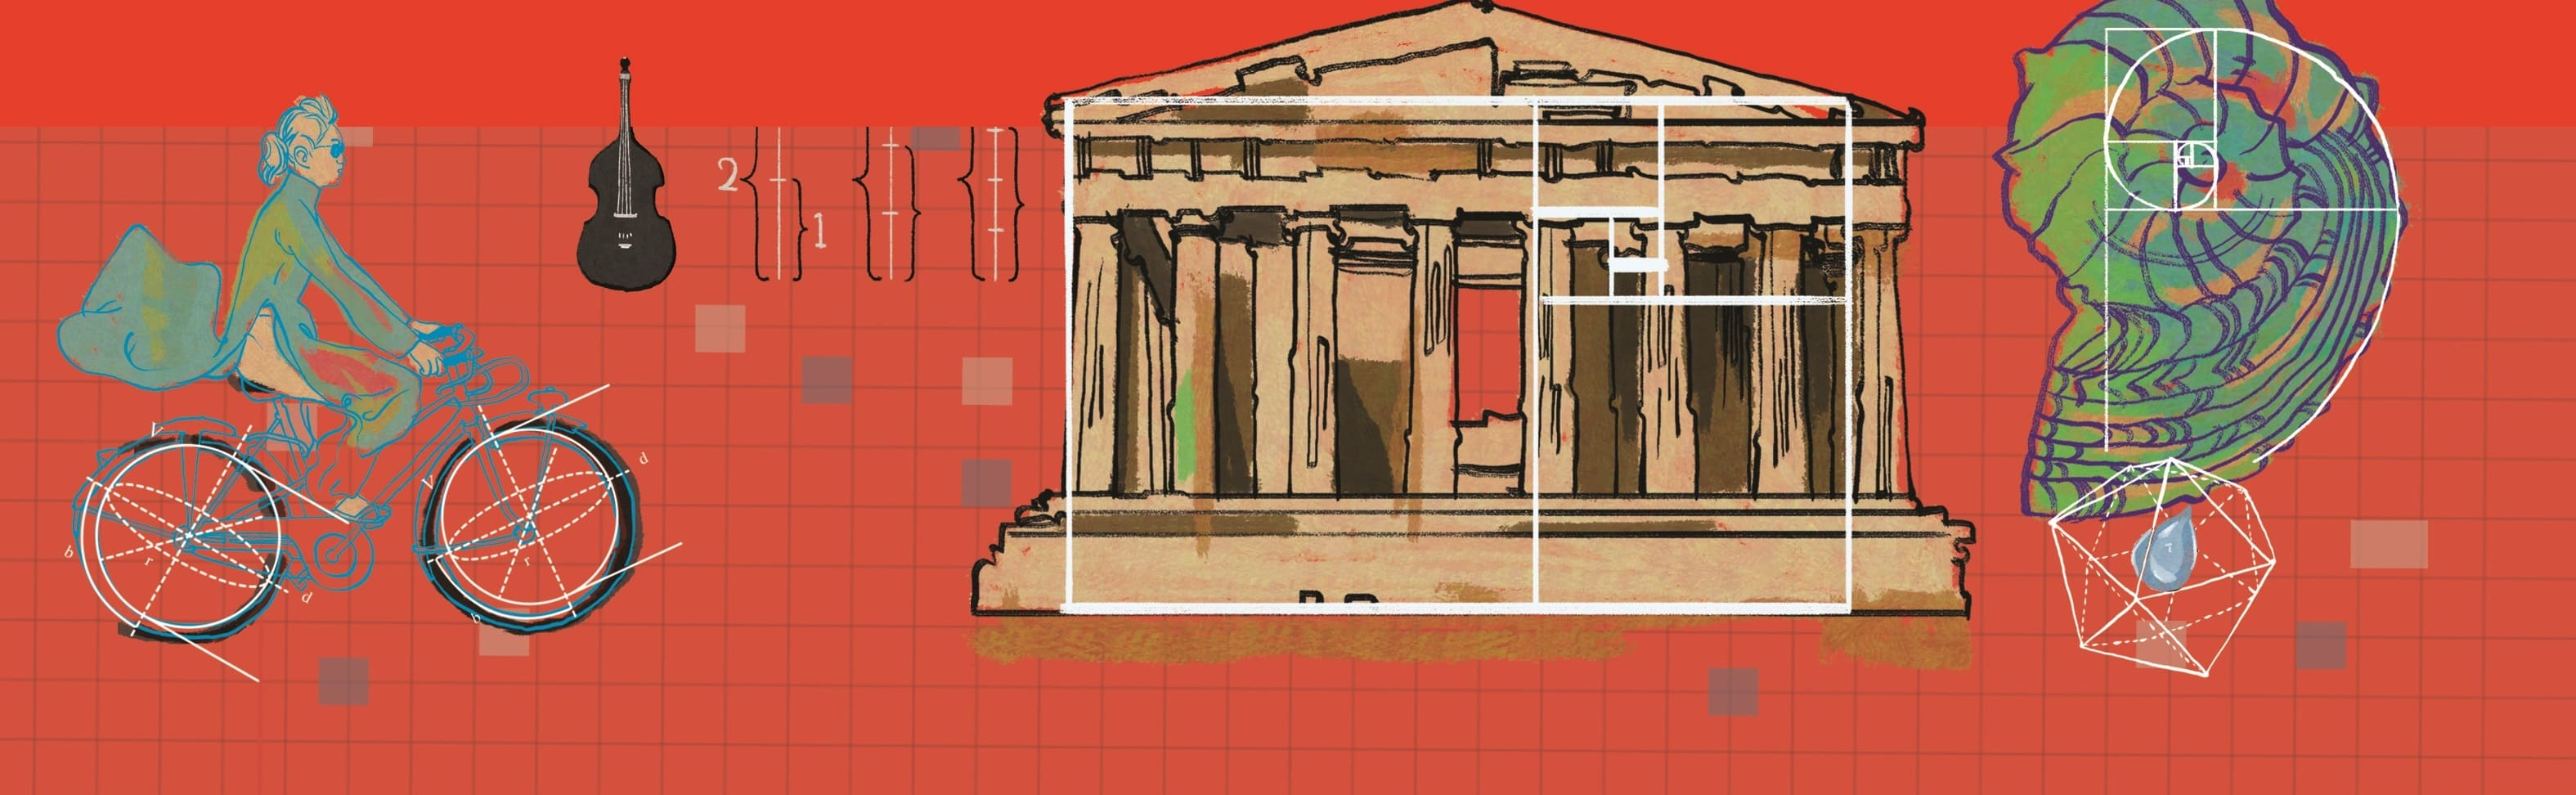
\includegraphics[width=19.3cm]{../bannertoanhocdoisong}}}
\AddToShipoutPicture*{\put(135,540){
\includegraphics[scale=1]{../tieude2.pdf}}}
\centering
\endgroup

\vspace*{165pt}
\begin{multicols}{2}
	\textit{Nhà thiên văn học, nhà thống kê và doanh nhân bảo hiểm người Đan Mạch Thorvald Thiele đã tìm ra cách sinh tự động các họa tiết khảm rất đẹp nhờ sử dụng khái niệm thặng dư bậc hai trong tập hợp các số nguyên\linebreak Gauss.}
	\vskip 0.1cm
	Tranh khảm gồm nhiều viên hoặc mảnh nhỏ nhiều màu sắc, làm từ những vật liệu khác nhau, được sắp xếp thành một họa tiết trang trí. Được dùng để lát sàn, trang trí tường, trần nhà và các đồ vật, tranh khảm rất được ưa chuộng ở thời Cổ Đại, và vẫn còn được sử dụng trong suốt thời Trung Cổ và Phục Hưng.
	\vskip 0.1cm
	Sau khi gần như biến mất, nghệ thuật lát khảm trở nên phổ biến trở lại với trào lưu nghệ thuật \textit{Art nouveau$^4$}  vào cuối thế kỷ $19$, đầu thế kỷ $20$. Những khám phá khoa học thu hút mạnh mẽ sự chú ý của công chúng và nhiều nghệ sỹ (gồm nhà thơ, nhạc sỹ, họa sỹ, v.v.) đã chuyển tải sức quyến rũ này bằng cách đưa thêm một chiều toán học vào tác phẩm của mình. Sự đều đặn duyên dáng của những họa tiết khảm tô điểm cho những ngôi nhà riêng cũng như những tòa nhà công cộng của chúng ta chỉ là một trong rất nhiều biểu hiện của cuộc tìm tòi thẩm mỹ này.
	\vskip 0.1cm
	Thorvald Thiele ($1838$ -- $1910$) đã đóng góp vào\, trào lưu\, này theo\, cách của\, riêng mình.
	\begin{figure}[H]
		\vspace*{-5pt}
		\centering
		\captionsetup{labelformat= empty, justification=centering}
		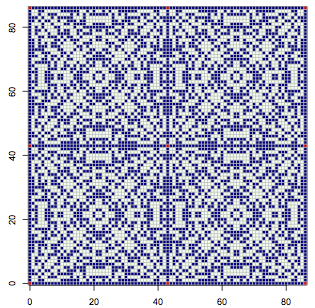
\includegraphics[width= 0.5\linewidth]{mosaique-1.png}
		\caption{\small\textit{\color{toanhocdoisong}Hình $1$. Thặng dư bậc hai modulo $43$.}}
		\vspace*{-10pt}
	\end{figure}
	Ông là người đầu tiên chỉ ra cách sử dụng thặng dư trong tập hợp các số nguyên Gauss để xây dựng một cách dễ dàng những hình khảm tuyệt đẹp. Trong Hình $2$ là hai họa tiết được ông công bố lần đầu tiên tại một hội nghị khoa học lớn của vùng Scandinavia tổ chức tại Copenhagen vào năm $1873$. Còn trong Hình $3$ là họa tiết Thiele ở sàn tiền sảnh Bộ Quốc phòng Đan Mạch, cũng ở Copenhagen.
	\begin{figure}[H]
		\vspace*{-5pt}
		\centering
		\captionsetup{labelformat= empty, justification=centering}
		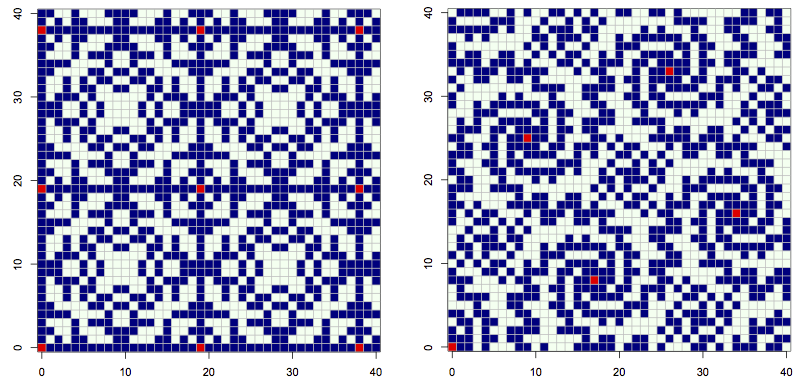
\includegraphics[width= 0.9\linewidth]{mosaique-2.png}
		\caption{\small\textit{\color{toanhocdoisong}Hình $2$. Hai họa tiết được Thiele công bố tại hội nghị khoa học năm $1873$.}}
		\vspace*{-5pt}
	\end{figure}
	Không chỉ tạo ra kết quả tuyệt đẹp, kỹ thuật xây dựng họa tiết khảm của Thiele vừa đơn giản lại vừa khéo léo. Nó dựa trên khái niệm thặng dư bậc hai phức mà chúng ta sẽ cùng nhau tìm hiểu dưới đây. Ở cuối bài, chúng ta sẽ đưa ra ba câu đố chưa có lời giải về họa tiết trong Hình $3$.
	\begin{figure}[H]
		\vspace*{-5pt}
		\centering
		\captionsetup{labelformat= empty, justification=centering}
		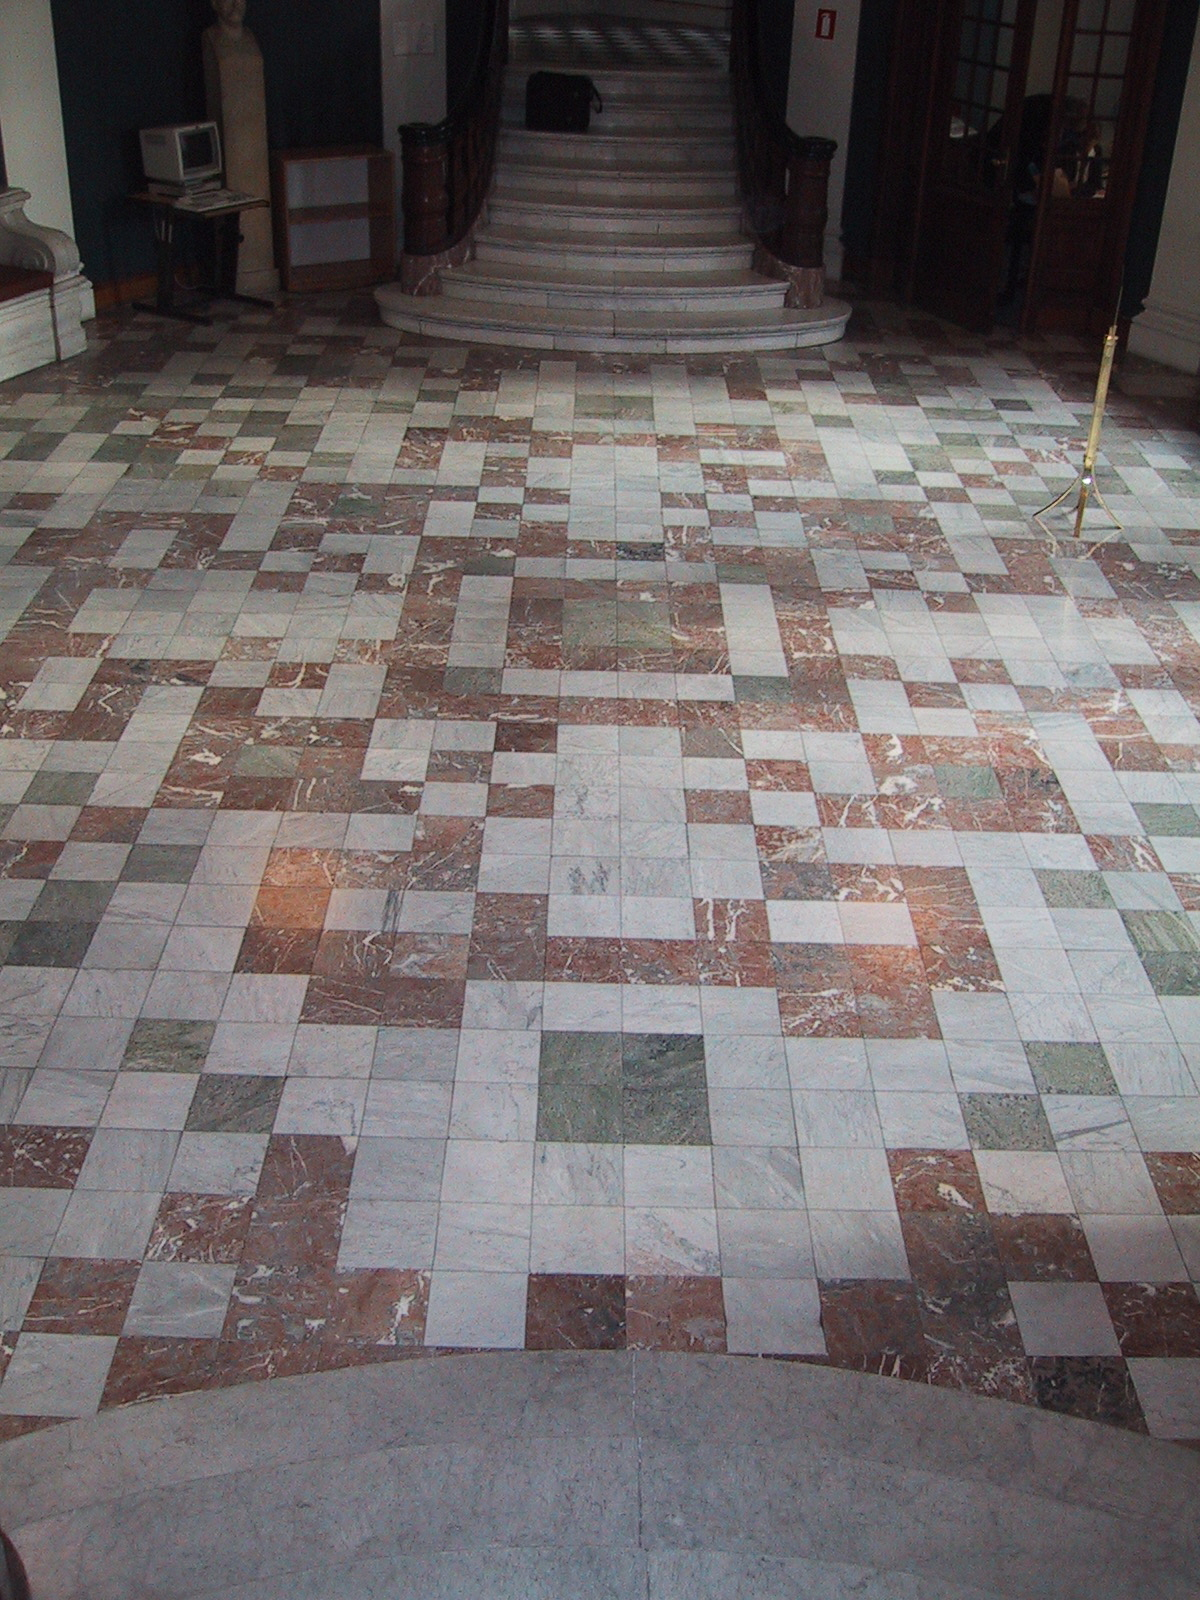
\includegraphics[width= 0.65\linewidth]{mosaique-3}
		\caption{\small\textit{\color{toanhocdoisong}Hình $3$. Họa tiết Thiele trang trí tiền sảnh Bộ Quốc Phòng Đan Mạch, số $9$ phố Holmens Kanal, Copenhagen.}}
		\vspace*{-10pt}
	\end{figure}
	\textbf{\color{toanhocdoisong}Đồng dư và thặng dư bậc hai trong $\pmb{\mathbb Z}$}
	\vskip 0.1cm
	Cho số nguyên $p \ge 1$. Nhắc lại rằng hai số nguyên
	\setlength{\abovedisplayskip}{5pt}
	\setlength{\belowdisplayskip}{5pt}
	\begin{align*}
		a, b \in \mathbb Z = \{ 0, \pm 1, \pm 2, \dots \}
	\end{align*}
	được gọi là đồng dư với nhau modulo $p$ nếu hiệu $a - b$ là bội của $p$, nghĩa là tồn tại $k \in \mathbb Z$ sao cho $a - b = kp$. Khi đó ta viết
	\begin{align*}
		a \equiv b \mod{p}.
	\end{align*}
	Nói riêng, $a$ đồng dư với số dư của nó khi chia cho $p$. Chẳng hạn, ta có thể viết $17 \equiv 1 \mod{4}$ vì $17 - 1 = 16$ chia hết cho $4$, hoặc $28 \equiv 0 \mod{4}$ vì $28 = 4 \times 7$ là bội của $4$.
	\vskip 0.1cm
	Ngoài ra, ta nói rằng số tự nhiên $q \in \mathbb N = \{ 0, 1, 2, \dots \}$ là một {\em thặng dư bậc hai} modulo $p$ nếu tồn tại số nguyên $x$ sao cho
	\begin{align*}
		q \equiv x^2 \mod{p}.
	\end{align*}
	Trong trường hợp ngược lại, ta nói $q$ không phải là thặng dư bậc hai modulo $p$.
	\vskip 0.1cm
	\textbf{\color{toanhocdoisong}Hai ví dụ đơn giản}
	\vskip 0.1cm
	\textbf{\color{toanhocdoisong}Ví dụ} $1.$ Mọi số tự nhiên $q$ đều là thặng dư bậc hai modulo $2$. Thật vậy:
	\vskip 0.1cm
	$\bullet$	Nếu $q \equiv 0 \mod{2}$, tức $q$ chẵn, thì $q \equiv 0^2 \mod{2}$;
	\vskip 0.1cm
	$\bullet$	Nếu $q \equiv 1 \mod{2}$, tức $q$ lẻ, thì $q \equiv 1^2 \mod{2}$.
	Một cách tổng quát, với mọi $p$, mọi số tự nhiên $q$ đồng dư với $0$ hoặc $1$ đều là thặng dư bậc hai modulo $p$.
	\vskip 0.1cm
	\textbf{\color{toanhocdoisong}Ví dụ} $2.$
	\vskip 0.1cm
	$\bullet$	Nếu $q \equiv 0 \mod{4}$, thì $q \equiv 0^2 \mod{4}$;
	\vskip 0.1cm
	$\bullet$	Nếu $q \equiv 1 \mod{4}$, thì $q \equiv 1^2 \mod{4}$.
	\vskip 0.1cm
	Trong khi đó, nếu $q \equiv 2 \mod{4}$ hoặc $q \equiv 3 \mod{4}$, không tồn tại số nguyên $x$ nào sao cho $q \equiv x^2 \mod{4}$. Điều này có thể được chứng minh bằng cách xét hai trường hợp $x$ chẵn và $x$ lẻ:
	\vskip 0.1cm
	$\bullet$	Nếu $x = 2n$ thì $x^2 = 4 n^2 \equiv 0 \mod{4}$;
	\vskip 0.2cm
	$\bullet$	Nếu $x = 2n + 1$ thì $x^2 = 4 n^2 + 4n + 1 \equiv 1 \mod{4}$.
	\vskip 0.2cm
	\textbf{\color{toanhocdoisong}Vỉa hè Thiele}
	\vskip 0.2cm
	Kết quả trên được minh họa trong Hình $4$ bằng ``vỉa hè Thiele". Một cách tổng quát, vỉa hè Thiele modulo $p$ gồm các mảnh hình vuông đơn vị đặt chính giữa các điểm $(0, 0)$, $(1, 0)$, $(2, 0)$, v.v. Màu của mảnh hình vuông tại điểm $(q, 0)$ được xác định như sau:
	\vskip 0.1cm
	$\bullet$	đỏ nếu $q \equiv 0 \mod{p}$;
	\vskip 0.1cm
	$\bullet$	xanh nếu $q$ là thặng dư bậc hai modulo $p$ (nhưng $q \not\equiv 0 \mod{p}$);
	\vskip 0.1cm
	$\bullet$	trắng nếu $q$ không phải thặng dư bậc hai modulo $p$.
	\begin{figure}[H]
		\vspace*{-5pt}
		\centering
		\captionsetup{labelformat= empty, justification=centering}
		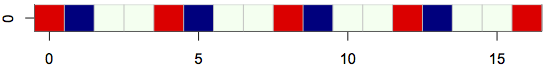
\includegraphics[width= 1\linewidth]{mosaique-4.png}
		\caption{\small\textit{\color{toanhocdoisong}Hình $4$. Vỉa hè Thiele modulo $4$.}}
		\vspace*{-10pt}
	\end{figure}
	Khi $p = 4$, mọi số tự nhiên $q$ đồng dư với $0$, $1$, $2$ hoặc $3$ modulo $4$. Họa tiết ``đỏ, xanh, trắng, trắng" ứng với các mảnh $(0, 0)$, $(1, 0)$, $(2, 0)$, $(3, 0)$ lặp lại vô hạn. Với mọi giá trị $p \ge 1$ khác, vỉa hè Thiele modulo $p$ có thể được xây dựng dễ dàng một khi ta đã biết màu của các mảnh $(0, 0), \dots, (p - 1, 0)$: họa tiết lặp lại với chu kỳ $p$.
	\vskip 0.2cm
	Các họa tiết khảm Thiele dựa trên một nguyên lý tương tự. Với mỗi cặp số nguyên $p = (p_1, p_2)$, màu của mảnh $(q_1, q_2)$ sẽ phụ thuộc vào việc $(q_1, q_2)$ có phải là thặng dư bậc hai modulo $p$ hay không. Để điều này có nghĩa, trước tiên chúng ta cần tìm hiểu khái niệm đồng dư giữa hai cặp số nguyên.
	\begin{tBox}
		\textbf{\textit{\color{toanhocdoisong}Thorvald Nicolai Thiele $\pmb{(1838 \!-\! 1910)}$}}
		\vskip 0.2cm
		\begin{wrapfigure}{l}{0.4\textwidth}
			\vspace*{-14pt}
			\centering
			\captionsetup{labelformat= empty, justification=centering}
			\hspace*{3pt}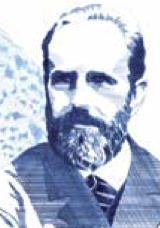
\includegraphics[width= 1.1\linewidth]{Thiele.png}
			\vspace*{-20pt}
		\end{wrapfigure}
		Thorvald Thiele sinh ngày $24$ tháng $12$ năm $1838$ ở Copenhagen và mất ngày $26$ tháng $9$ năm $1910$ ở cùng thành phố, thọ $71$ tuổi. Tên ông được đặt theo cha đỡ đầu của ông, nhà điêu khắc Bertel Thorvaldsen. Sau quá trình học tập xuất sắc, ông trở thành giáo sư thiên văn học tại Đại học Copenhagen từ năm $1875$ đến năm $1907$, đồng thời là giám đốc đài thiên văn của trường. Được coi là một người mở đường của thống kê toán học, ông là người đầu tiên đề xuất một lý thuyết chuyển động Brown, đồng thời là tác giả của các khái niệm cumulant và hàm hợp lý. Thiele cũng góp phần sáng lập Hafnia, công ty bảo hiểm nhân thọ tư nhân đầu tiên của của Đan Mạch, vào năm $1872$. Ông là giám đốc khoa học của công ty tới năm $1901$, rồi chủ tịch Hội đồng Quản trị từ năm $1903$ tới năm $1910$. Tên ông được đặt cho hai tiểu hành tinh; một trong  hai tiểu hành tinh đó được phát hiện bởi con trai ông, Holger Thiele, cũng là một nhà thiên văn học nổi tiếng.
	\end{tBox}
	\textbf{\color{toanhocdoisong}Mở rộng cho tập hợp các số nguyên Gauss}
	\vskip 0.1cm
	Trong công trình \textit{Disquisitiones arithmeticae\footnote[5]{\color{toanhocdoisong}Công ty phá sản năm $1993$.}}  xuất bản năm $1801$, nhà toán học, vật lý học và thiên văn học người Đức Carl Friedrich Gauss ($1777$ -- $1855$) quan tâm đến số học đồng dư trên những tập hợp khác $\mathbb Z$, trong đó có tập hợp các cặp số nguyên, tức là các vector $(a_1, a_2) \in \mathbb Z^2 = \mathbb Z \times \mathbb Z$.
	\vskip 0.1cm
	Gauss định nghĩa tổng và tích của hai phần tử bất kỳ $a = (a_1, a_2)$, $b = (b_1, b_2)$ trong $\mathbb Z^2$ như sau:
	\begin{align*}
		&(a_1, a_2) + (b_1, b_2) \\
		= \,&(a_1 + b_1, a_2 + b_2), \\
		&(a_1, a_2) \times (b_1, b_2) \\
		= \,&(a_1  b_1 - a_2  b_2, a_1  b_2 + a_2  b_1).
	\end{align*}
	Phép cộng là phép cộng vector thông thường. Phép nhân, có vẻ bí ẩn hơn, liên hệ mật thiết với khái niệm số phức (xem phần đóng khung bên dưới).
	\vskip 0.1cm
	Tập hợp $\mathbb Z^2$ được trang bị hai phép toán trên được gọi là tập hợp các {\em số nguyên Gauss}. Tập hợp các số nguyên Gauss có đủ các tính chất cần thiết để ta có thể định nghĩa trên đó các khái niệm đồng dư và thặng dư bậc hai tương tự những khái niệm đã có trên $\mathbb Z$.
	\vskip 0.1cm
	Cho hai số tự nhiên $p_1$ và $p_2$ không đồng thời bằng $0$. Ta nói rằng hai phần tử $a, b \in \mathbb Z$ đồng dư với nhau modulo $p = (p_1, p_2)$ nếu tồn tại $k = (k_1, k_2) \in \mathbb Z^2$ sao cho $a - b = k \times p$. Nói cách khác, $a \equiv b \mod{p}$ nếu và chỉ nếu
	\begin{align*}
		&(a_1, a_2) - (b_1, b_2) \\
		= \,&(k_1 p_1 - k_2 p_2, k_1 p_2 + k_2 p_1).
	\end{align*}
	Ta nói rằng $q = (q_1, q_2)$ là một {\em thặng dư bậc hai phức} modulo $p = (p_1, p_2)$ nếu tồn tại $x = (x_1, x_2) \in \mathbb Z^2$ sao cho $q \equiv x^2 \mod{p}$. Nói cách khác, ta cần tìm các số nguyên $x_1$ và $x_2$ sao cho
	\begin{align*}
		(q_1, q_2) \equiv (x_1^2 - x_2^2, 2 x_1 x_2) \mod{p}.
	\end{align*}
	\vskip 0.1cm
	\begin{tBox}
		\textbf{\textit{\color{toanhocdoisong}Mối liên hệ với số phức}}
		\vskip 0.1cm
		\begin{wrapfigure}{r}{0.4\linewidth}
			\vspace*{-15pt}
			\centering
			\captionsetup{labelformat= empty, justification=centering}
			\hspace*{-12pt}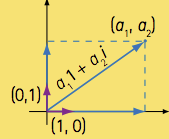
\includegraphics[width= 1.15\linewidth]{mosaique-6.png}
			\vspace*{-15pt}
		\end{wrapfigure}
		Các phép toán được Gauss định nghĩa trong $\mathbb Z^2$ có liên hệ mật thiết với khái niệm số phức. Một số phức là một số có dạng $a_1 + a_2 i$, ở đó $i = \sqrt{-1}$. Số phức có thể được biểu diễn trong mặt phẳng bằng cách đặt $1 = (1, 0)$ và $i = (0, 1)$, sao cho $(a_1, a_2) = a_1 1 + a_2 i$, mà ta có thể viết gọn là $a_1 + a_2 i$ mà không sợ nhầm lẫn. Thực hiện phép cộng và phép nhân thông thường với các biểu thức đại số $a_1 + a_2 i$ và $b_1 + b_2 i$, ta được:
		\begin{align*}
			&(a_1 + a_2 i) + (b_1 + b_2i) \\
			= \,&(a_1 + b_1) + (a_2 + b_2) i, \\
			&(a_1 + a_2i) \times (b_1 + b_2i) \\
			= \,&a_1 b_1 + (a_1 b_2 + a_2 b_1) i + a_2 b_2 i^2 \\
			= \,&( a_1  b_1 - a_2  b_2) + (a_1 b_2 + a_2 b_1) i ,
		\end{align*}
		ở đó ta đã thay $i^2 = -1$.
		\vskip 0.1cm
		Để ý rằng phép nhân với $i$ tương đương với phép quay một góc $\pi / 2$ ngược chiều kim đồng hồ. Thật vậy:
		\begin{align*}
			(a_1 + a_2 i) \times i = a_1 i + a_2 i^2 = -a_2 + a_1 i.
		\end{align*}
		\begin{wrapfigure}{r}{0.4\linewidth}
			\vspace*{-15pt}
			\centering
			\captionsetup{labelformat= empty, justification=centering}
			\hspace*{-12pt}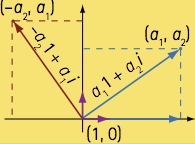
\includegraphics[width= 1.1\linewidth]{mosaique-7.png}
			\vspace*{-15pt}
		\end{wrapfigure}
		Khi $a_2 = 0$, số là {\em số thực}, còn khi $a_1 = 0$, số là {\em số ảo}.
		Các phép toán được định nghĩa trong tập hợp các số phức chính là các phép toán trong tập hợp các số nguyên Gauss. Tập hợp $\mathbb Z^2$ cùng với hai phép toán này thường được ký hiệu là $\mathbb Z[i]$.
	\end{tBox}
	\vskip 0.1cm
	\textbf{\color{toanhocdoisong}Hình khảm Thiele}
	\vskip 0.1cm
	Cũng như vỉa hè Thiele, một hình khảm Thiele modulo $p = (p_1, p_2)$ gồm nhiều mảnh hình vuông đơn vị phủ kín mặt phẳng. Màu của mảnh tại điểm $q = (q_1, q_2)$ được xác định như sau:
	\vskip 0.1cm
	$\bullet$	đỏ nếu $q \equiv 0 \mod{p}$;
	\vskip 0.1cm
	$\bullet$	xanh nếu $q$ là thặng dư bậc hai phức modulo $p$ (nhưng $q \not\equiv 0 \mod{p}$);
	\vskip 0.1cm
	$\bullet$	trắng nếu $q$ không phải thặng dư bậc hai phức modulo $p$.
	\vskip 0.1cm
	Ví dụ, giả sử $p = (2, 0)$. Ta có:
	\begin{align*}
		&(a_1, a_2) \equiv (b_1, b_2) \mod{p} \\
		\iff& a_1 - b_1 = 2 k_1 \mbox{ và } a_2 - b_2 = 2 k_2,
	\end{align*}
	tức là $a_1 \equiv b_1 \mod{2}$ và $a_2 \equiv b_2 \mod{2}$. Suy ra với mọi $(a_1, a_2) \in \mathbb Z^2$, $(a_1, a_2) \equiv (0, 0), (0, 1), (1, 0)$ hoặc $(1, 1) \mod{p = (2, 0)}$.
	\vskip 0.1cm
	Từ nhận xét trên, để xây dựng hình khảm Thiele tương ứng, ta chỉ cần xét xem $(0, 0), (0, 1), (1, 0)$ và $(1, 1)$ có phải thặng dư bậc hai phức modulo $p = (2, 0)$ hay không.
	\vskip 0.1cm
	Như vậy, với $a_1, a_2 \in \{0, 1\}$, ta cần kiểm tra xem có tồn tại hay không $x_1, x_2 \in \mathbb Z$ sao cho
	\begin{align*}
		a_1 \equiv x_1^2 - x_2^2 \mod{2}, a_2 \equiv 2 x_1 x_2 \mod{2}.
	\end{align*}
	Nếu $a_2 = 0$, chỉ cần chọn $x_1 = a_1$ và $x_2 = 0$. Nhưng nếu $a_2 = 1$ thì không thể tìm được $x_1, x_2 \in \mathbb Z$ thỏa mãn vì $2 x_1 x_2$ luôn chẵn.
	\vskip 0.1cm
	Kết quả này được mình họa trong Hình $5$. Các mảnh $(0, 0)$, $(1, 0)$, $(0, 1)$ và $(1, 1)$ tạo thành họa tiết cơ bản (bên trái) mà chúng ta có thể lặp lại một số lần tùy ý (bên phải). Hiệu ứng ảo giác của hình vẽ được tạo bởi sự tuần hoàn kép (cả chiều ngang lẫn chiều dọc) của họa tiết cùng với các màu sắc tương phản mạnh.
	\begin{figure}[H]
		\vspace*{-5pt}
		\centering
		\captionsetup{labelformat= empty, justification=centering}
		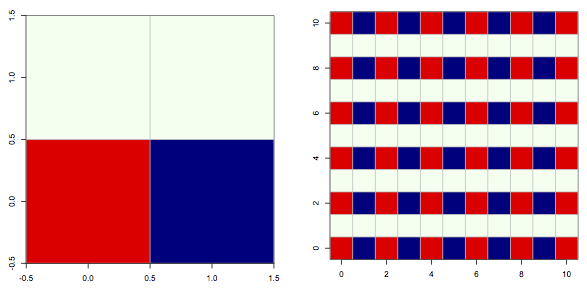
\includegraphics[width= 1\linewidth]{mosaique-8.png}
		\caption{\small\textit{\color{toanhocdoisong}Hình $5$. Hình khảm Thiele modulo $p = (2, 0)$.}}
		\vspace*{-10pt}
	\end{figure}
	Hai thí dụ khác, do chính Thiele đưa ra, được trình bày trong Hình $2$ (hình này được vẽ bằng một phần mềm miễn phí, với hướng dẫn tải và sử dụng ở cuối bài). Hình khảm bên trái tương ứng với $p = (19, 0)$; có thể dễ dàng nhận thấy nó tuần hoàn theo chiều dọc và chiều ngang. Hình khảm bên phải tương ứng với $p = (17, 8)$; chúng ta cũng nhận có sự đều đặn, nhưng việc xác định chính xác nó thì không hiển nhiên như trường hợp trước.
	\vskip 0.1cm
	\textbf{\color{toanhocdoisong}Ý nghĩa hình học}
	\vskip 0.1cm
	Để hiểu rõ hơn quy luật của hình khảm Thiele, chúng ta hãy coi các phần tử của $\mathbb Z^2$ như các vector tọa độ nguyên. Để ý rằng theo định nghĩa, hai vector $a = (a_1, a_2)$ và $b = (b_1, b_2)$ đồng dư với nhau modulo $p = (p_1, p_2)$ nếu và chỉ nếu
	\begin{align*}
		&(a_1, a_2) - (b_1, b_2) \\
		= \,&(k_1 p_1 - k_2 p_2, k_1 p_2 + k_2 p_1) \\
		= \,&k_1 (p_1, p_2) + k_2 (-p_2, p_1) ,
	\end{align*}
	nghĩa là nếu hiệu của chúng có thể viết thành tổng của một bội của $p$ và một bội của vector $p' = (-p_2, p_1)$ vuông góc với $p$.
	\vskip 0.1cm
	Trong ngôn ngữ hình học, điều này có nghĩa là hai vector $a$ và $b$ đồng dư với nhau modulo $p$ nếu có thể đi từ $a$ tới $b$ (hoặc ngược lại) bằng một số hữu hạn các tịnh tiến theo $p$, $-p$, $p'$ và $-p'$. Đặc biệt, tất cả các vector [trong $\mathbb Z^2$] đều đồng dư với một vector nằm trong hình vuông có bốn đỉnh $(0, 0)$, $p$, $p'$ và $p + p'$. Tính chất này là tương đương trong $\mathbb Z^2$ của phép chia có dư trong $\mathbb Z$.
	\vskip 0.1cm
	Quay trở lại với hình bên phải của Hình $2$, chúng ta có thể kiểm tra rằng họa tiết cơ bản quả đúng là phần được giới hạn bởi bốn điểm đỏ $(9, 25)$, $(17, 8)$, $(26, 33)$ và $(34, 16)$.
	\vskip 0.1cm
	\PIbox{\textbf{\color{toanhocdoisong}\textit{Có bao nhiêu mảnh được tô màu?}}
		\vskip 0.1cm
		Kinh nghiệm cho thấy những hình khảm Thiele đẹp nhất khi $p = (p_1, p_2)$ là một {\em số nguyên tố Gauss}, nghĩa là nếu với mọi $a, b \in \mathbb Z^2$:
		\begin{align*}
			&a \times b \equiv (0, 0) \mod{p} \\
			\implies &a \equiv (0, 0) \mbox{ hoặc } b \equiv (0, 0) \mod{p}.
	\end{align*}}
	\PIbox{
		Có thể chứng minh được rằng $p$ là số nguyên tố Gauss nếu và chỉ nếu một trong ba điều kiện sau được thỏa mãn (chúng ta thừa nhận kết quả này):
		\vskip 0.1cm
		$\bullet$	Nếu $p_1 \ge 1$ và $p_2 \ge 1$: $p_1^2 + p_2^2$ là số nguyên tố theo nghĩa thông thường;
		\vskip 0.1cm
		$\bullet$	Nếu $p_1 = 0$ và $p_2 \ge 1$: $|p_2|$ nguyên tố và $|p_2| \equiv 3 \mod{4}$;
		\vskip 0.1cm
		$\bullet$	Nếu $p_1 \ge 1$ và $p_2 = 0$: $|p_1|$ nguyên tố và $|p_1| \equiv 3 \mod{4}$.
		\vskip 0.1cm
		Như vậy, $(19, 0)$, $(71, 0)$ và $(17, 8)$ là các số nguyên tố Gauss, nhưng $(5, 0)$ thì không phải, và ta có $(5, 0) = (1, 2) \times (1, -2)$.
		\vskip 0.1cm
		Ta biết rằng nếu $p$ là một số nguyên tố, một nửa các số từ $1$ đến $p - 1$ là thặng dư bậc hai modulo $p$. Nói cách khác, có $(p - 1) / 2$ mảnh màu xanh trong họa tiết cơ bản của vỉa hè Thiele modulo $p$. Tương tự, bằng cách sử dụng các khái niệm trong lý thuyết trường, có thể chứng minh rằng nếu $p = (p_1, p_2)$ là số nguyên tố Gauss với $p_1 \ge 1$ và $p_2 \ge 1$, thì có $p_1^2 + p_2^2 - 1$ mảnh màu xanh trong họa tiết cơ bản của hình khảm Thiele modulo $p$.}
	\vskip 0.2cm
	\textbf{\color{toanhocdoisong}Trở lại bức hình tiền sảnh}
	\vskip 0.1cm
	Sàn sảnh trong Hình $3$ được lát theo hình khảm Thiele modulo $(71, 0)$. Họa tiết cơ bản của nó được cho trong Hình $6$. Ngày nay thuộc Bộ Quốc phòng Đan Mạch, tòa nhà có sàn lát này từng là trụ sở của công ty bảo hiểm Hafnia. Ở cương vị chủ tịch Hội đồng Quản trị của công ty, Thiele đã cho phép khởi công xây tòa nhà vào tháng $5$ năm $1910$, chỉ vài tháng trước khi ông qua đời ở tuổi $71$. Người ta cho rằng họa tiết lát sảnh được chọn sau khi Thiele mất, để tưởng nhớ ông.
	\vskip 0.1cm
	Chúng ta có thể rút ra ba quan sát về hình lát sàn này như sau:
	\vskip 0.1cm
	$\bullet$ Có một số lỗi trong việc thể hiện họa tiết. Thực vậy, mặc dù $(27, 35)$ là thặng dư bậc hai modulo $p = (71, 0)$, viên gạch lát tương ứng lại có màu trắng. Đây có thể là một lỗi tính toán, vì nó xuất hiện đến bảy lần trên toàn bộ tác phẩm.
	\begin{figure}[H]
		\vspace*{-5pt}
		\centering
		\captionsetup{labelformat= empty, justification=centering}
		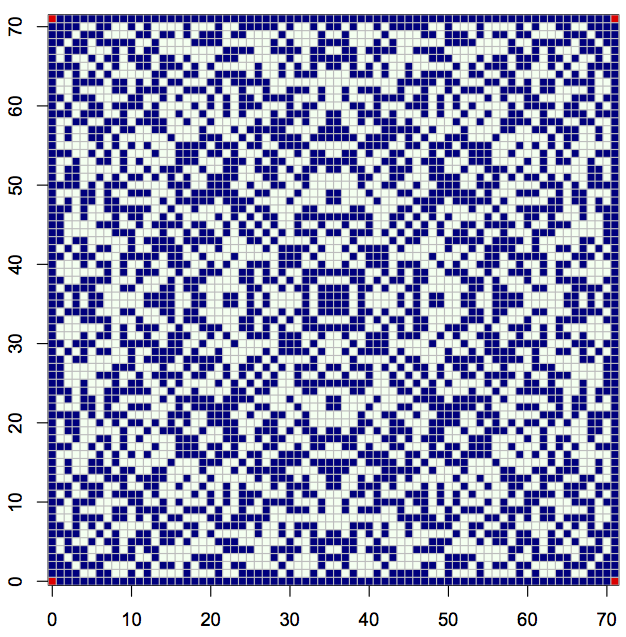
\includegraphics[width= 0.85\linewidth]{mosaique-9.png}
		\caption{\small\textit{\color{toanhocdoisong}Hình $6$. Hình khảm Thiele modulo $(71, 0)$, được dùng làm mẫu lát sàn tiền sảnh Bộ Quốc phòng Đan Mạch.}}
		\vspace*{-10pt}
	\end{figure}
	$\bullet$ Khi so sánh Hình $3$ và Hình $6$, chúng ta thấy mảnh $(25, 45)$ đúng ra phải màu trắng, nhưng trên sàn gạch thực tế lại màu đỏ. Lỗi này không lặp lại ở những chỗ khác. Không rõ đây là do sự lơ đãng của người thợ lát, hay do truyền thống nghề nghiệp không muốn sự hoàn hảo?
	\begin{figure}[H]
		\vspace*{-5pt}
		\centering
		\captionsetup{labelformat= empty, justification=centering}
		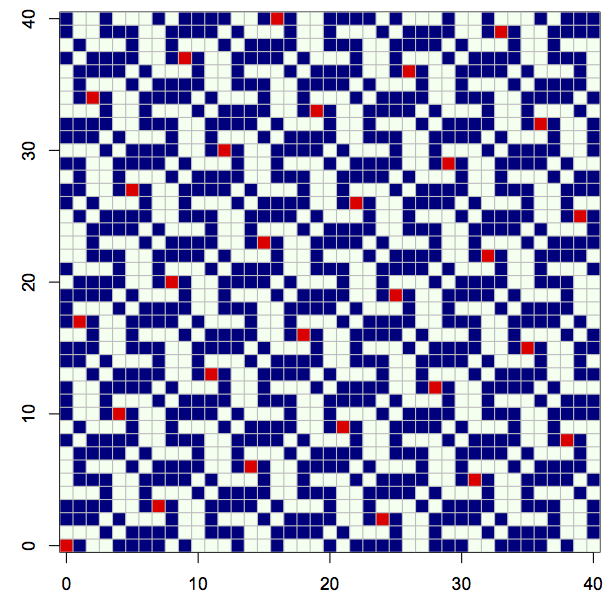
\includegraphics[width= 0.85\linewidth]{mosaique-10.png}
		\caption{\small\textit{\color{toanhocdoisong}Hình $7$. Thặng dư bậc hai modulo $(7, 3)$. Hình khảm này được tạo với một số không nguyên tố: $(7, 3) = (1, -1) \times (2, 5)$.}}
		\vspace*{-10pt}
	\end{figure}
	$\bullet$ Vì sao một số viên gạch tương ứng với thặng dư bậc hai có màu đỏ, trong khi những viên khác lại xanh lá cây? Liệu có phải chỉ đơn giản vì lý do thẩm mỹ? Tính cân đối của họa tiết gợi ý rằng hai màu này thể hiện một tính chất khác của các thặng dư bậc hai. Nhưng đó là tính chất gì?
	\vskip 0.1cm
	Có thể lục lại các tài liệu lưu trữ của công ty Hafnia để tìm câu trả lời cho hai câu hỏi đầu tiên. Câu hỏi thứ ba thì có bản chất thuần túy toán học và việc giải đáp nó có thể cần đến các tính chất của các số nguyên Gauss, của thặng dư bậc hai (hay bậc bốn?) phức và các chủ đề hấp dẫn khác của lý thuyết số. Câu trả lời vẫn là bí ẩn, và việc tìm ra nó được dành cho các bạn!
	\vskip 0.2cm
	\PIbox{
	\textbf{\color{toanhocdoisong}\textit{Vẽ tranh khảm Thiele bằng R}}
	\vskip 0.1cm
	Chúng ta có thể dễ dàng tạo ra một hình khảm Thiele nhờ một chương trình được viết bởi S{\o}ren Buhl, giáo sư toán và thống kê, Đại học Aalborg (Đan Mạch). Chương trình của ông được viết bằng ngôn ngữ R, có thể được tải miễn phí cho Windows, MacOS hoặc Linux tại:
	\url{http://www.r-project.org/}
	\vskip 0.1cm
	Chương trình vẽ có thể được tải ở đây:
	\url{http://www.math.mcgill.ca/cgenest/Thiele.R}
	\vskip 0.1cm
	Sau khi sao chép đoạn mã của chương trình vào cửa sổ lệnh của R, ta có thể vẽ một hình khảm Thiele modulo $p$ với kích thước $(n + 1) \times (n + 1)$ bằng lệnh $tuile(p, n)$. Thí dụ, Hình $2$ là kết quả của các lệnh $tuile(19,40)$ và $tuile(17 + 8i, 40)$. Hình $5$ nhận được bằng cách nhập lệnh $tuile(71, 71)$.}
	\vskip 0.1cm
	\textbf{\color{toanhocdoisong}Tài liệu tham khảo}
	\vskip 0.1cm
	[$1$] Décaillot, A.--M. ($2002$). Géométrie des tissus, mosaïques, échiquiers: Mathématiques curieuses et utiles. \textit{Revue d'histoire des mathématiques}, vol. $8$, pp. $145-206$.
	\vskip 0.1cm
	[$2$] Lauritzen, S., \textit{Thiele: Pioneer in Statistics}, Oxford University Press, $2002$.
\end{multicols}
%	\newpage


%	\thispagestyle{empty}
%	\begingroup 
%	\AddToShipoutPicture*{\put(20,25){\includegraphics[width=18cm]{hoangtuy}}}
%	\centering
%	\vspace*{0cm}
%	\endgroup
%	\newpage	
%	\pagestyle{empty}
	
%	\setcounter{figure}{0}
%	\thispagestyle{duongvaotoanhocnone}
\pagestyle{duongvaotoanhoc}
\everymath{\color{duongvaotoanhoc}}
\graphicspath{{../duongvaotoanhoc/pic/}}
\blfootnote{$^1$\color{duongvaotoanhoc}Universit\'e Paris--Saclay.}
\begingroup
\AddToShipoutPicture*{\put(0,616){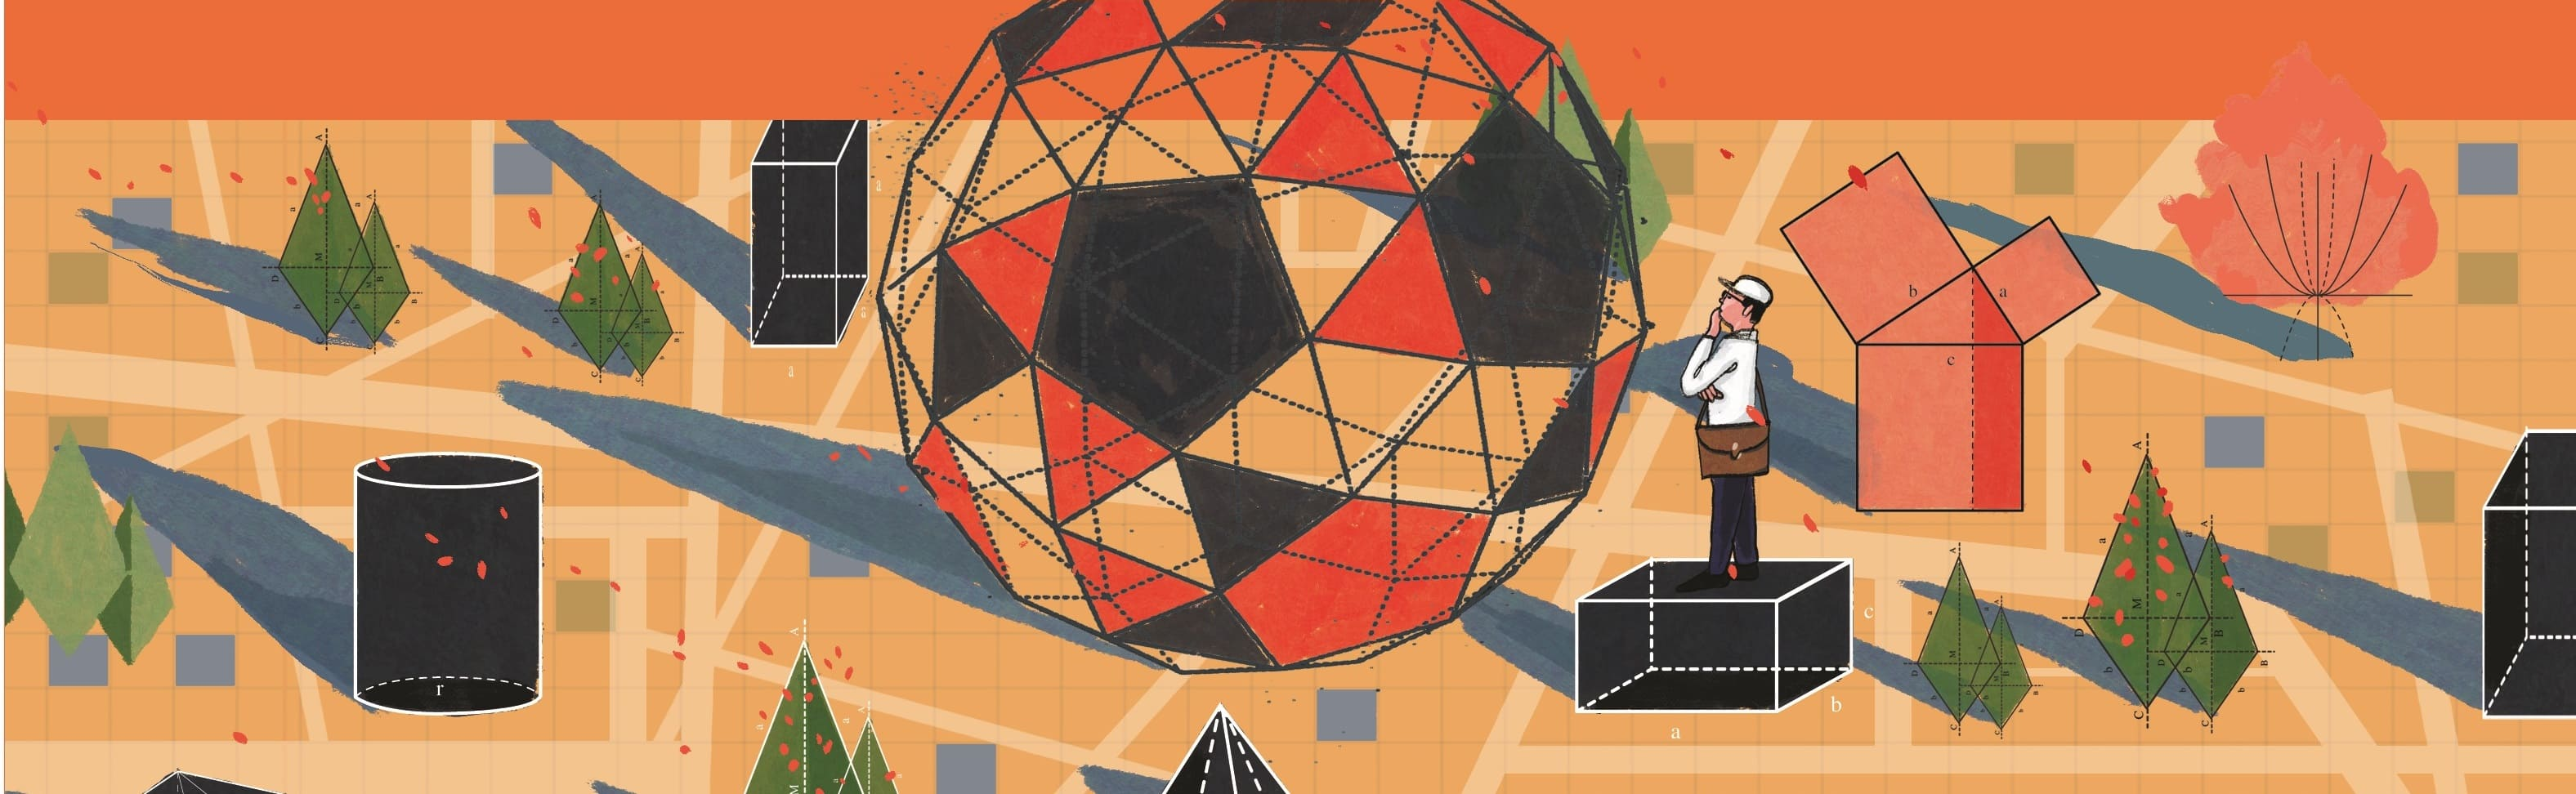
\includegraphics[width=19.3cm]{../bannerduongvao}}}
\AddToShipoutPicture*{\put(90,522){
\includegraphics[scale=1]{../tieude.pdf}}}
\centering
\endgroup
\vspace*{185pt}

\begin{multicols}{2}	
	Tôpô học là lĩnh vực nghiên cứu các không gian trừu tượng, những đối tượng liên tục. Ngược lại, số học là lĩnh vực nghiên cứu các số nguyên, những đối tượng rời rạc. Hai lĩnh vực này dường như nằm ở hai thái cực đối lập của toán học. Đấy là cho đến khoảng vài thập kỷ trở lại đây, khi các nhà toàn học phát hiện ra mối liên hệ giữa hai đối tượng tưởng như chẳng liên quan ở hai bên. Người ta đang xây dựng một cầu nối, một cuốn từ điển cho phép dịch các định lý từ một bên sang bên kia và ngược lại. Lĩnh vực mới toanh này được gọi là {\bf\color{duongvaotoanhoc} tôpô số học}.
	\vskip 0.1cm
	\textbf{\color{duongvaotoanhoc}Nhóm cơ bản}
	\vskip 0.1cm
	Để nói về tôpô số học, tất nhiên ta phải bắt đầu với... tôpô học và số học. Các không gian tôpô là các đối tượng cho phép ta nói về lân cận của các điểm, cũng như các hàm liên tục. Sự ``giống nhau'' giữa các không gian tôpô được cho bởi các {phép đồng phôi}, các hàm liên tục $1-1$ mà hàm ngược cũng liên tục. Để đơn giản, ta sẽ chỉ quan tâm đến các không gian {\bf\color{duongvaotoanhoc} liên thông}: hai điểm bất kỳ luôn nối được bằng một đường. Một {\bf\color{duongvaotoanhoc} đường} giữa hai điểm $x$, $y$ trong một không gian tôpô $X$ đơn giản là một hàm liên tục $f: I \to X$ sao cho $f(0) = x$ và $f(1) = y$.
	\vskip 0.1cm
	Giả sử ta có một đường khác $g: I \to X$ từ $x$ đến $y$. Không gì cản chúng ta nói về khái niệm ``đường giữa hai đường $f$ và $g$'', mà toán học gọi là {\bf\color{duongvaotoanhoc} đồng luân}. Đó là một hàm liên tục $H: I \times I \to X$ sao cho $H(t,0) = f(t)$, $H(t,1) = g(t)$, $H(0,s) = x$ và $H(1,s) = y$. Nói cách khác, $H$ là một họ các đường trung gian được tham số hóa bởi $s$, thể hiện sự biến dạng liên tục từ đường $f$ (khi $s=0$) đến đường $g$ (khi $s = 1$), đồng thời giữ cố dịnh hai đầu mút $x$, $y$. 
	\begin{figure}[H]
		\vspace*{-5pt}
		\centering
		\captionsetup{labelformat= empty, justification=centering}
		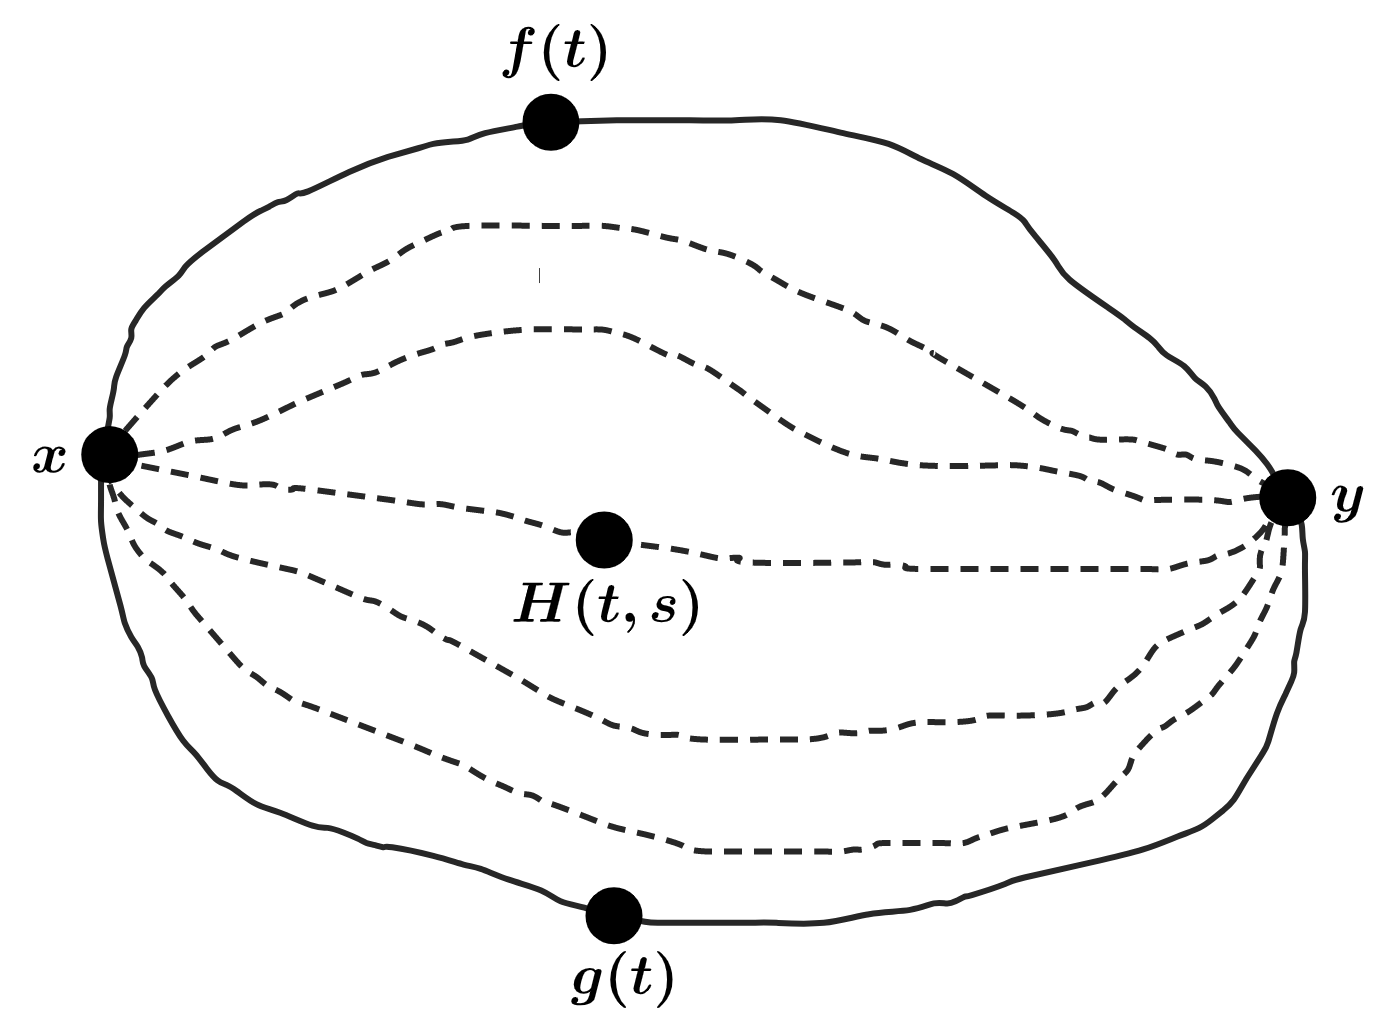
\includegraphics[width= 0.9\linewidth]{h1.png}
		\caption{\small\textit{\color{duongvaotoanhoc}Hình $1$: Một phép đồng luân giữa hai đường $f$ và $g$.}}
		\vspace*{-10pt}
	\end{figure}
	Khi $H$ tồn tại, ta nói hai đường $f$ và $g$ đồng luân, ký hiệu bởi $f \sim g$. Khi hai đường bất kỳ giữa hai điểm cho trước luôn đồng luân, ta nói không gian $X$ {\bf\color{duongvaotoanhoc} đơn liên}. Ví dụ về không gian đơn liên là không gian Euclid $\mathbb{R}^n$. Thật vậy, cấu trúc cộng và nhân với vô hướng trong $\mathbb{R}^n$ cho phép ta định nghĩa phép đồng luân $H(t,s) = (1-s) \cdot f(t) + s \cdot g(t)$ giữa hai đường $f, g$ tùy ý. Mặt  siêu cầu $\mathbb{S}^n$, thu được bằng cách thêm một điểm ở xa vô tận vào $\mathbb{R}^n$, cũng đơn liên với $n > 1$: hãy chọn một điểm P tùy ý trên mặt cầu và hình dung rằng mọi đường đều có thể biến dạng liên tục thành một đường không đi qua $P$. Mà $\mathbb{R}^n$ bỏ đi $P$ chính là (đồng phôi với) $\mathbb{R}^n$, nên hai đường không đi qua $P$ luôn đồng luân.
		\begin{figure}[H]
		\vspace*{-5pt}
		\centering
		\captionsetup{labelformat= empty, justification=centering}
		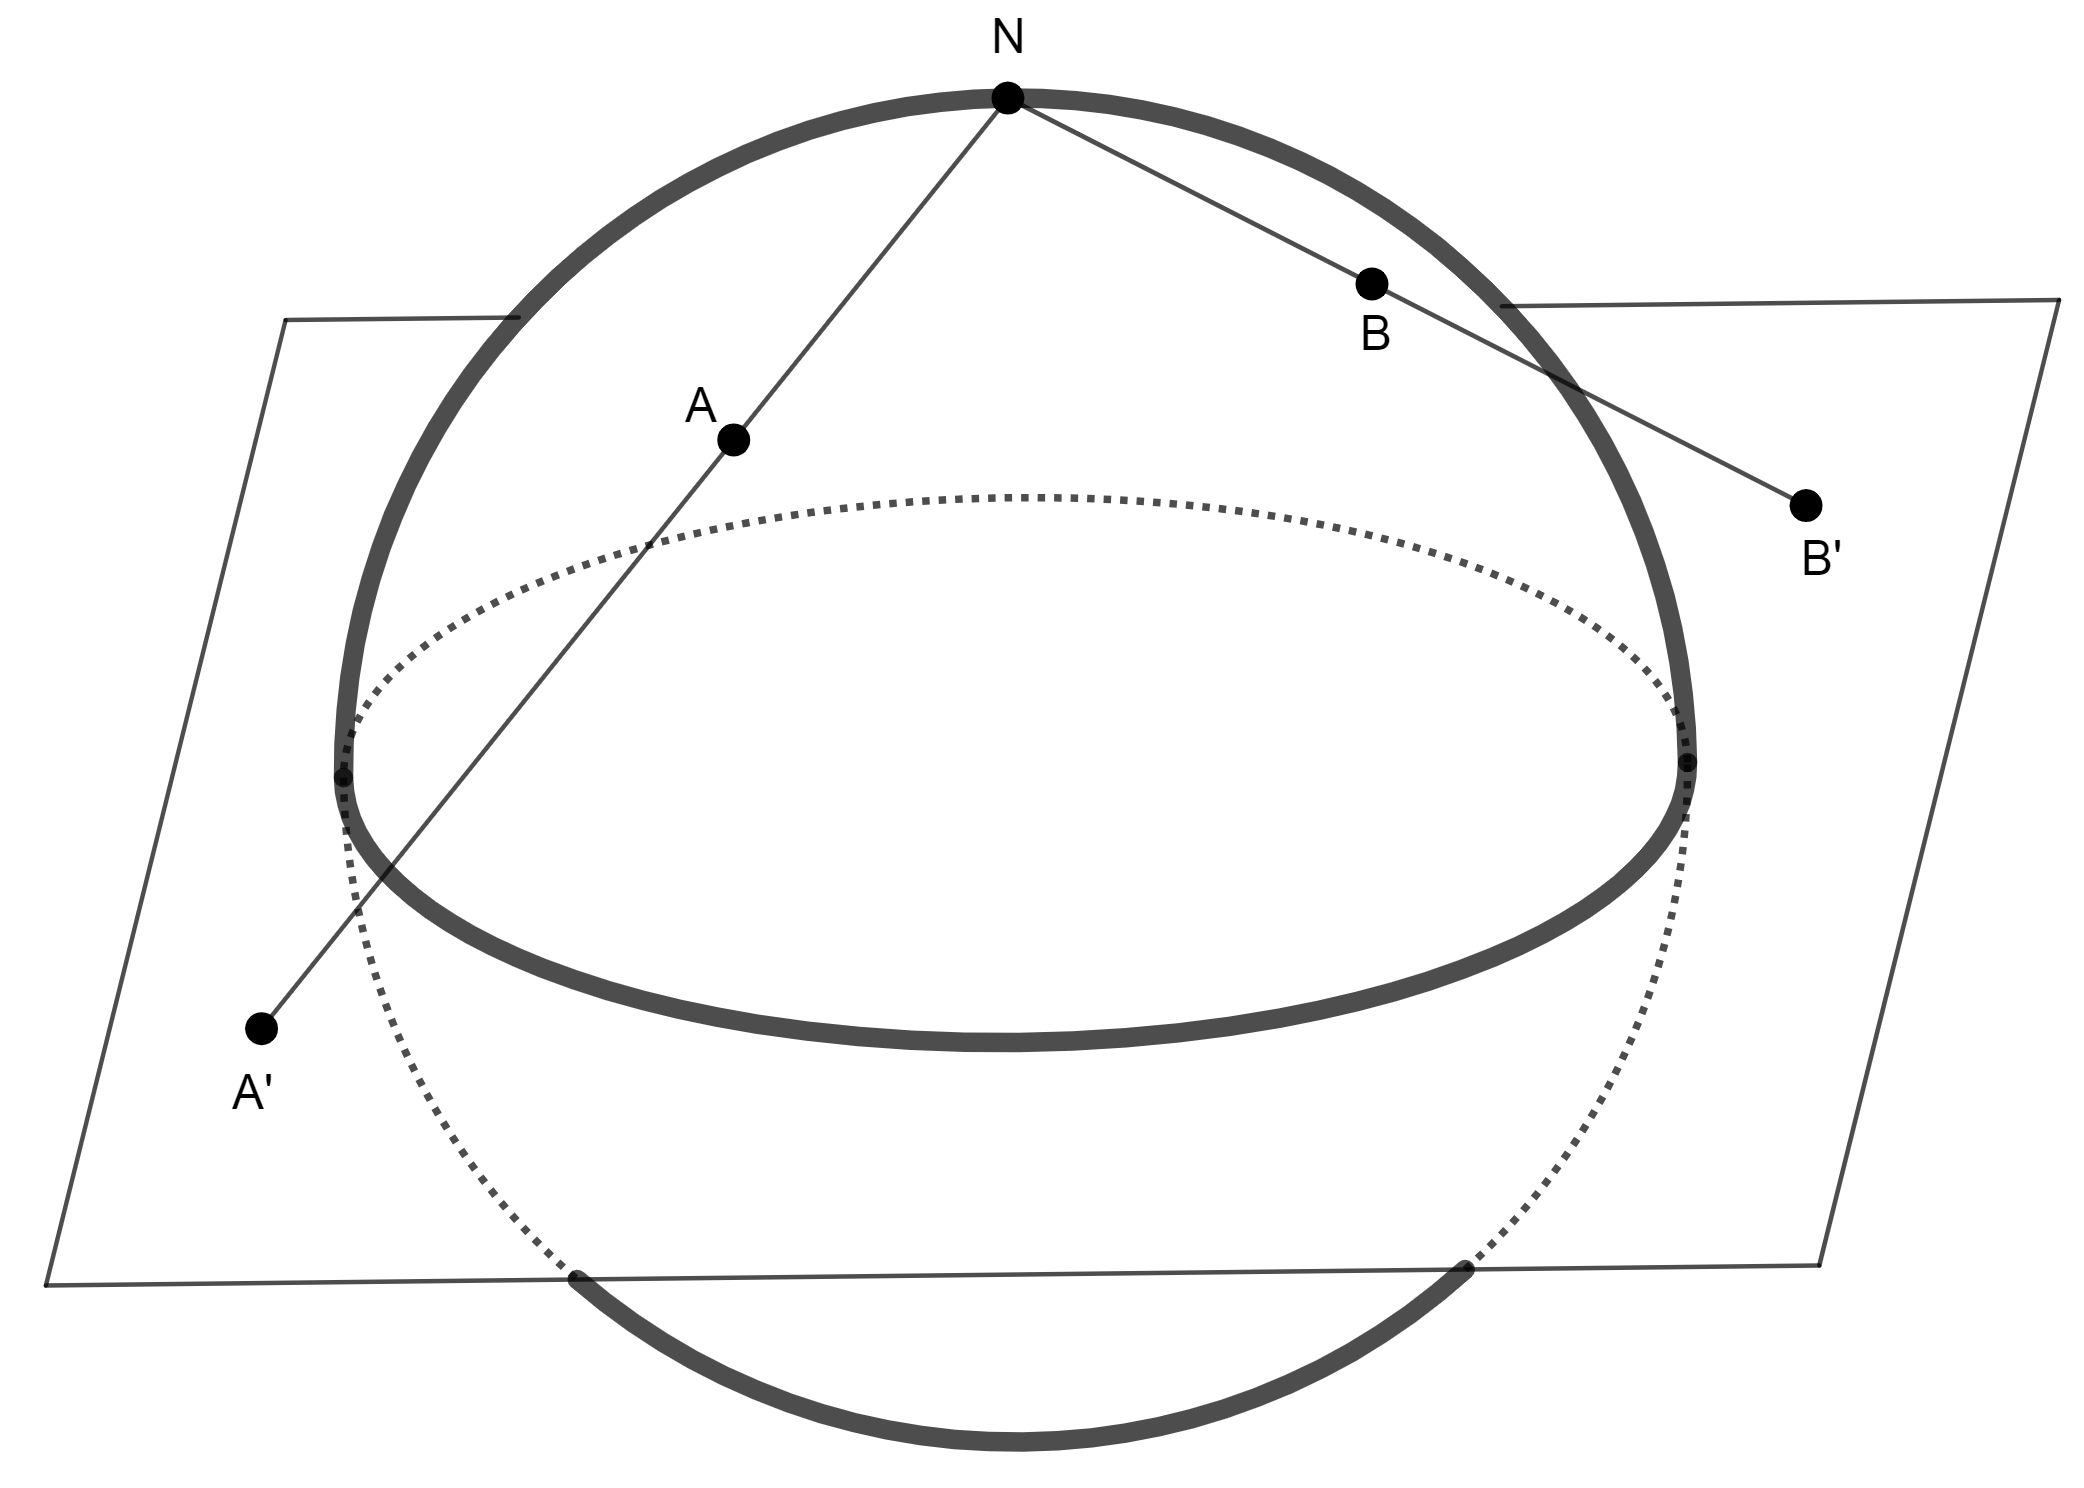
\includegraphics[width= 0.9\linewidth]{h2.png}
		\caption{\small\textit{\color{duongvaotoanhoc}Hình $2$: Qua phép chiếu lập thể, mặt cầu $\mathbb{S}^2$ bỏ đi điểm cực bắc $N$ trở thành mặt phẳng $\mathbb{R}^2$. Ta có thể xem $N$ như ``điểm ở xa vô tận'' của mặt phẳng.}}
		\vspace*{-10pt}
	\end{figure}
	Các đường cho ta bất biến đại số đầu tiên cho phép phân biệt các không gian tôpô (cho biết khi nào chúng không đồng phôi), được gọi là {\bf\color{duongvaotoanhoc} nhóm cơ bản}, định nghĩa bởi Henri Poincaré năm $1895$. Ta hãy cố định một điểm $x \in X$ và xét các đường từ $x$ đến chính nó, được gọi là các {\bf\color{duongvaotoanhoc} khuyên}. Ta xây dựng một phép toán trên chúng: cho $f$ và $g$ là hai khuyên tại $x$, ta định nghĩa $g \ast f: I \to X$ là khuyên thu được bằng cách đi theo $f$ với vận tốc gấp đôi rồi đi theo $g$ với vận tốc gấp đôi. Bằng công thức, 
	\begin{align*}
		(g \ast f)(t) \begin{cases}
			= f(2t) & \text{nếu } 0 \le t \le \frac{1}{2} \\
			= g(2t-1) & \text{nếu } \frac{1}{2} \le t \le 1.
		\end{cases}
	\end{align*}
	Như một thủ tục, ta cần kiểm tra các tiên đề của nhóm. Đầu tiên là tính kết hợp. Bằng tính toán trực tiếp, ta thấy ngay $h \ast (g \ast f) \neq (h \ast g) \ast f$. Tuy nhiên, hai đường này đồng luân. Điều này gợi ý rằng ta cần xem hai đường là như nhau nếu chúng đồng luân.
	\begin{figure}[H]
		\vspace*{5pt}
		\centering
		\captionsetup{labelformat= empty, justification=centering}
		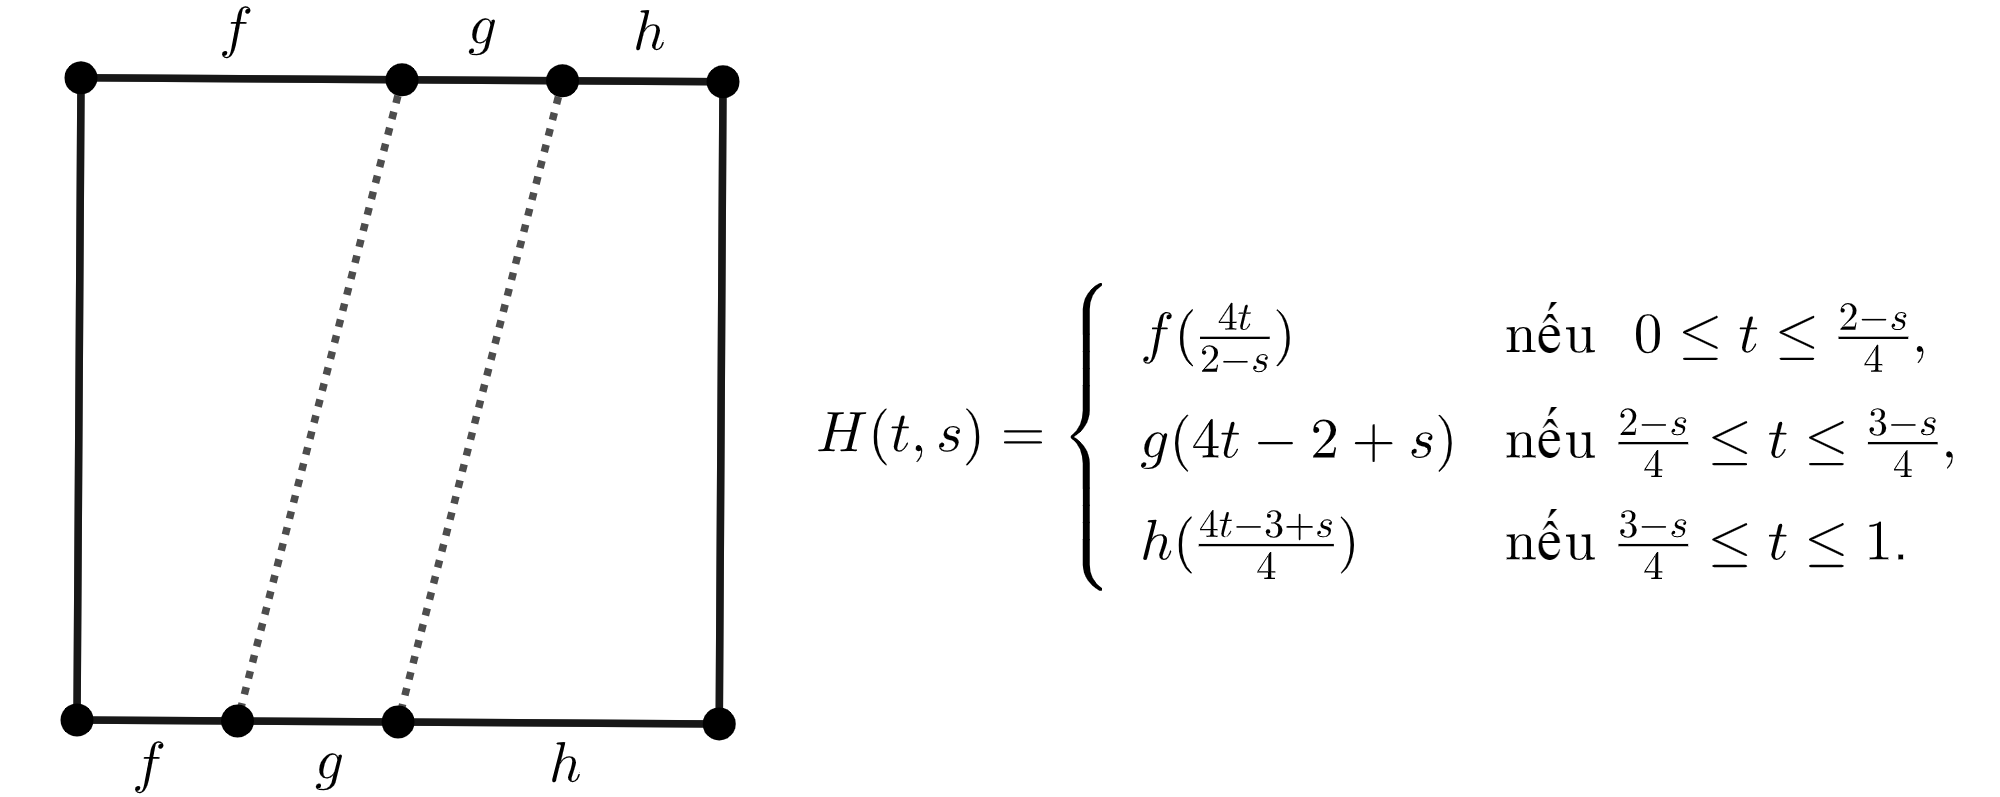
\includegraphics[width= 0.9\linewidth]{h3.png}
		\caption{\small\textit{\color{duongvaotoanhoc}Hình $3$: $h \ast (g \ast f) \sim (h \ast g) \ast f$.}}
		\vspace*{-10pt}
	\end{figure}
	Thứ hai, ta cần chỉ ra phần tử trung lập. Một cách trực giác, ta thấy nó phải là đường hằng $c$, cho bởi ``đứng yên tại $x$'', hay $c(t) = x$.
	\begin{figure}[H]
		\vspace*{-5pt}
		\centering
		\captionsetup{labelformat= empty, justification=centering}
		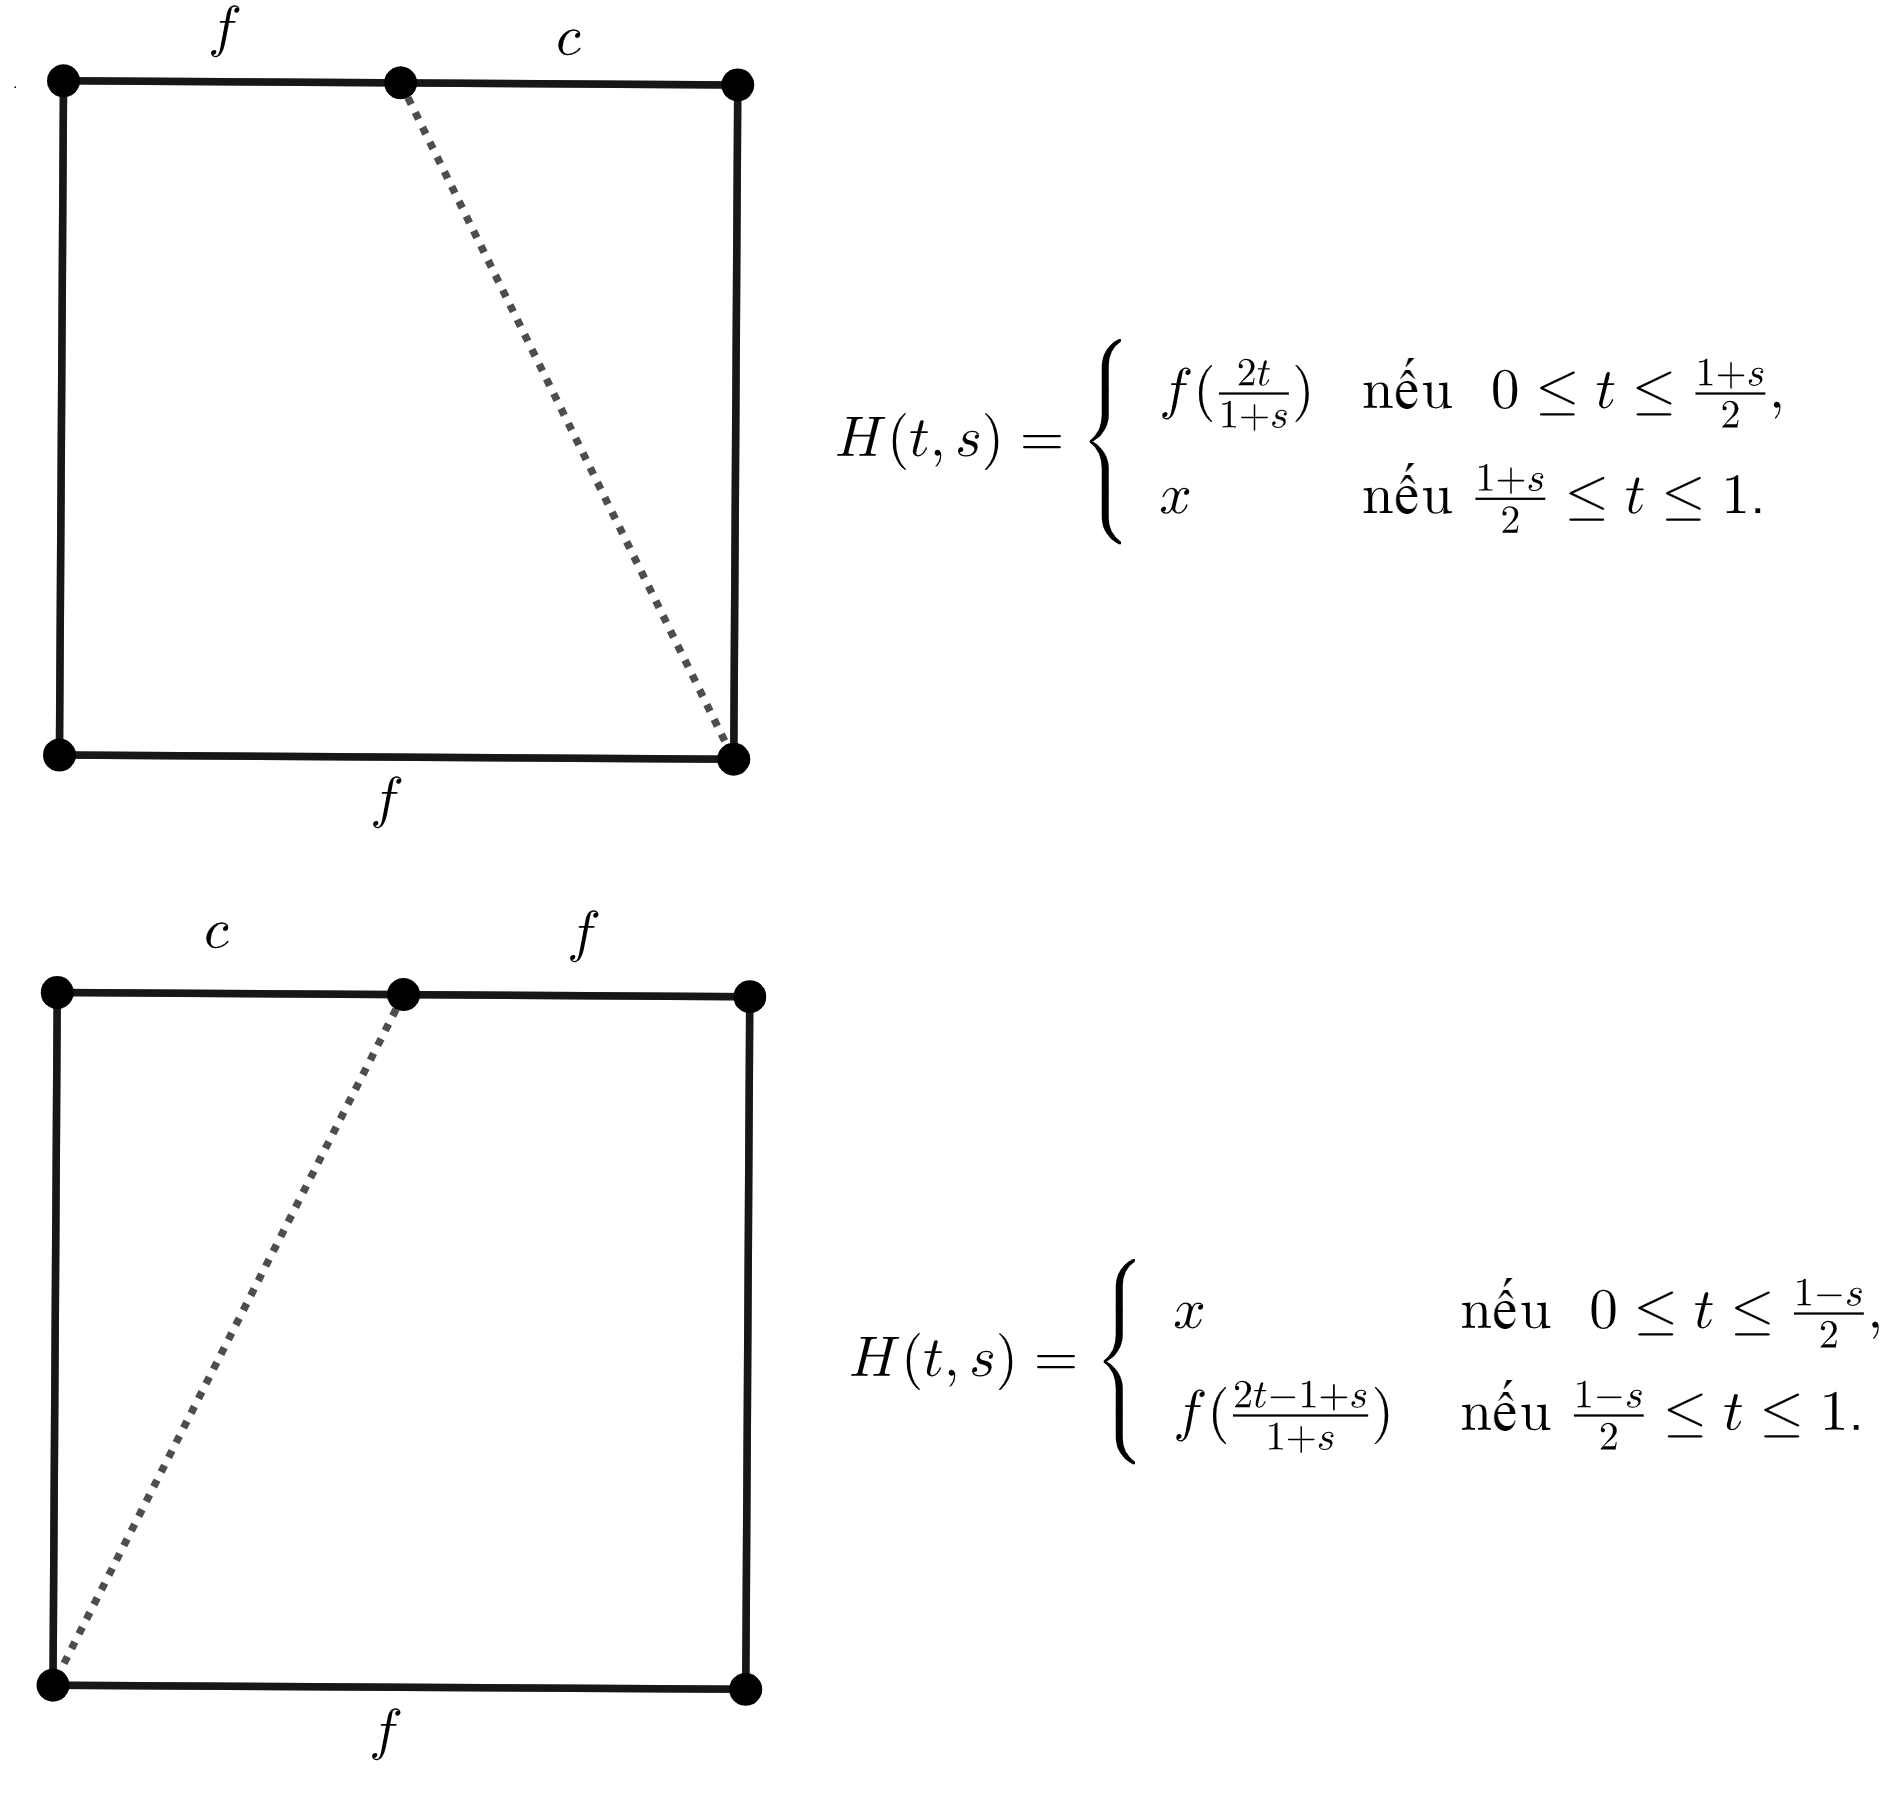
\includegraphics[width= 0.9\linewidth]{h4.png}
		\caption{\small\textit{\color{duongvaotoanhoc}Hình $4$: $f \ast c \sim f$ và $c \ast f \sim f$.}}
		\vspace*{-10pt}
	\end{figure}
	Cuối cùng, ta cần tìm nghịch đảo của một đường $f$ cho trước. Đó là đường $f'$ cho bởi ``đi ngược với $f$'', hay $f'(t) = f(1-t)$.
	\begin{figure}[H]
		\vspace*{-5pt}
		\centering
		\captionsetup{labelformat= empty, justification=centering}
		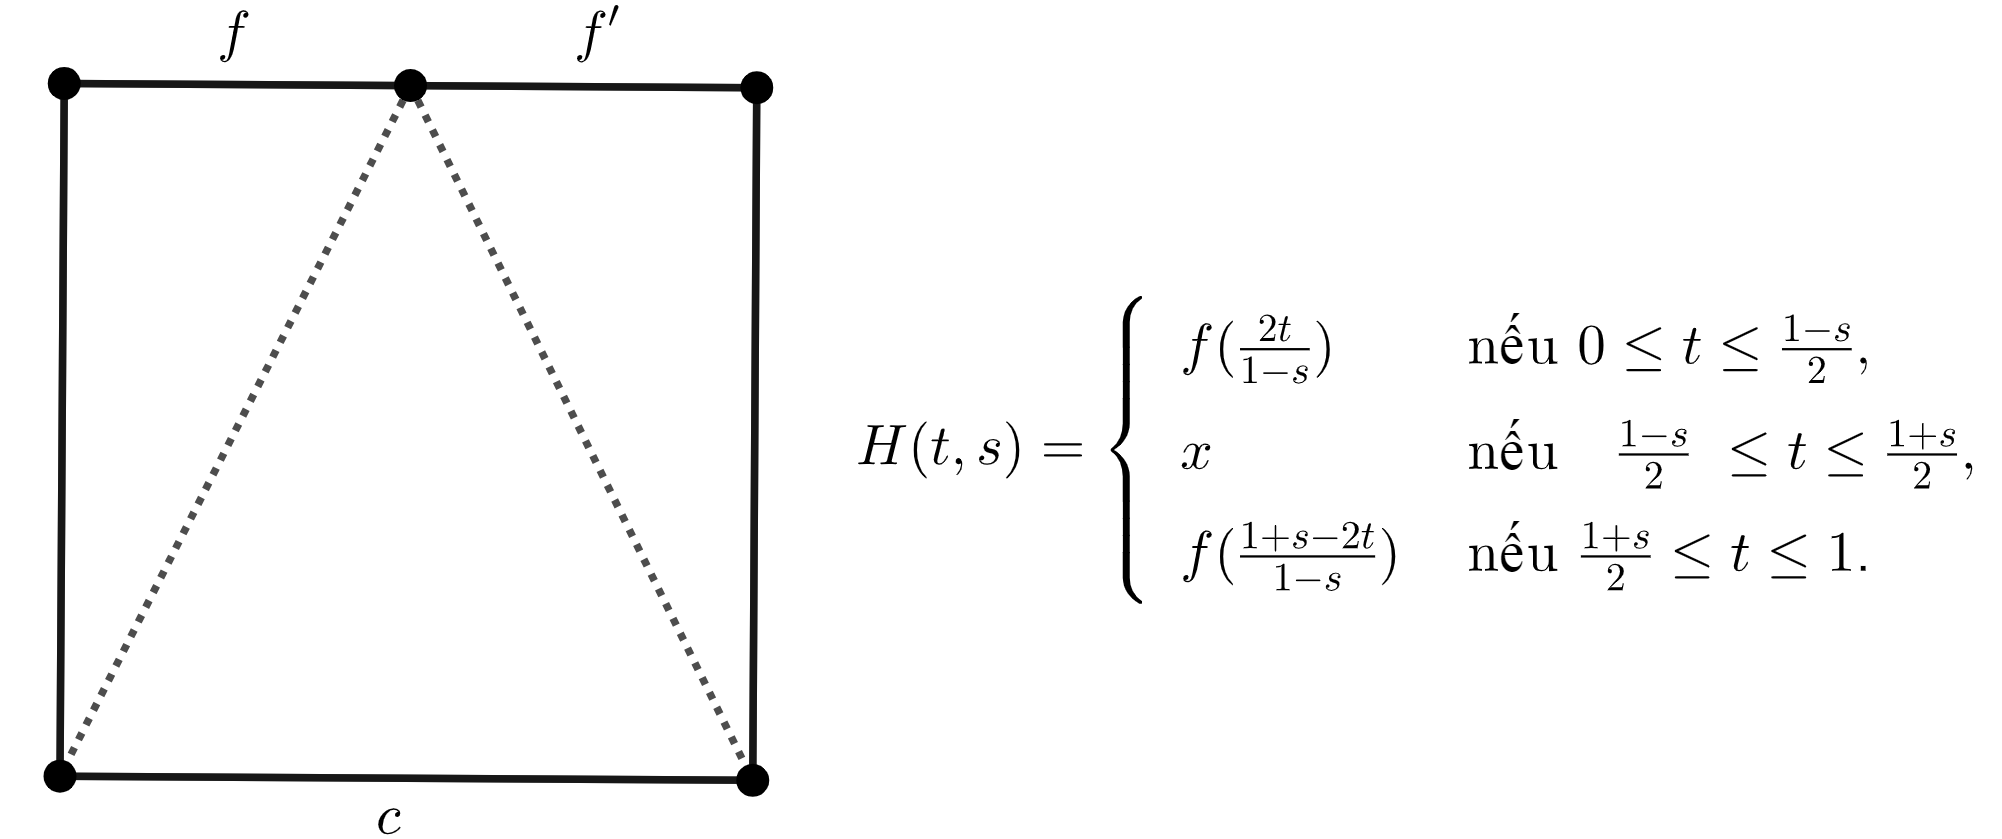
\includegraphics[width= 0.9\linewidth]{h5.png}
		\caption{\small\textit{\color{duongvaotoanhoc}Hình $5$: $f \ast f' \sim c$. Tất nhiên, vì $f'' = f$ nên $f' \ast f \sim c$.}}
		\vspace*{-10pt}
	\end{figure}
	Vậy các khuyên tại $x$ (sai khác đồng luân) tạo thành một nhóm, nó được gọi là nhóm cơ bản của $X$, ký hiệu bởi $\pi_1(X)$.
	\vskip 0.1cm
	Một không gian là đơn liên khi và chỉ khi nhóm cơ bản của nó tầm thường (mọi khuyên đều biến dạng liên tục được về một điểm). Chẳng hạn $\pi_1(\mathbb{R}^n) = 1$ và $\pi_1(\mathbb{S}^n) = 1$ với $n > 1$. Ví dụ không tầm thường đầu tiên là đường tròn $\mathbb{S}^1$, có thể xem như tập các số phức với môđun bằng $1$. Nhóm cơ bản của nó là (đẳng cấu với) $\mathbb{Z}$. Cụ thể, với mỗi số nguyên n, ta xét khuyên $f_n$ cho bởi $f_n(t) = \cos(2n \pi t)+i\cdot \sin(2n\pi t)$, đó là phép cuộn đoạn thẳng thành $|n|$ lần đường tròn (theo chiều dương nếu $n > 0$, theo chiều âm nếu $n < 0$). Một khuyên $f$ tùy ý đồng luân với $f_n$ khi và chỉ khi $f$ quay quanh đường tròn đúng $|n|$ lần với chiều tương ứng với dấu của $n$.
	\begin{figure}[H]
		\vspace*{-5pt}
		\centering
		\captionsetup{labelformat= empty, justification=centering}
		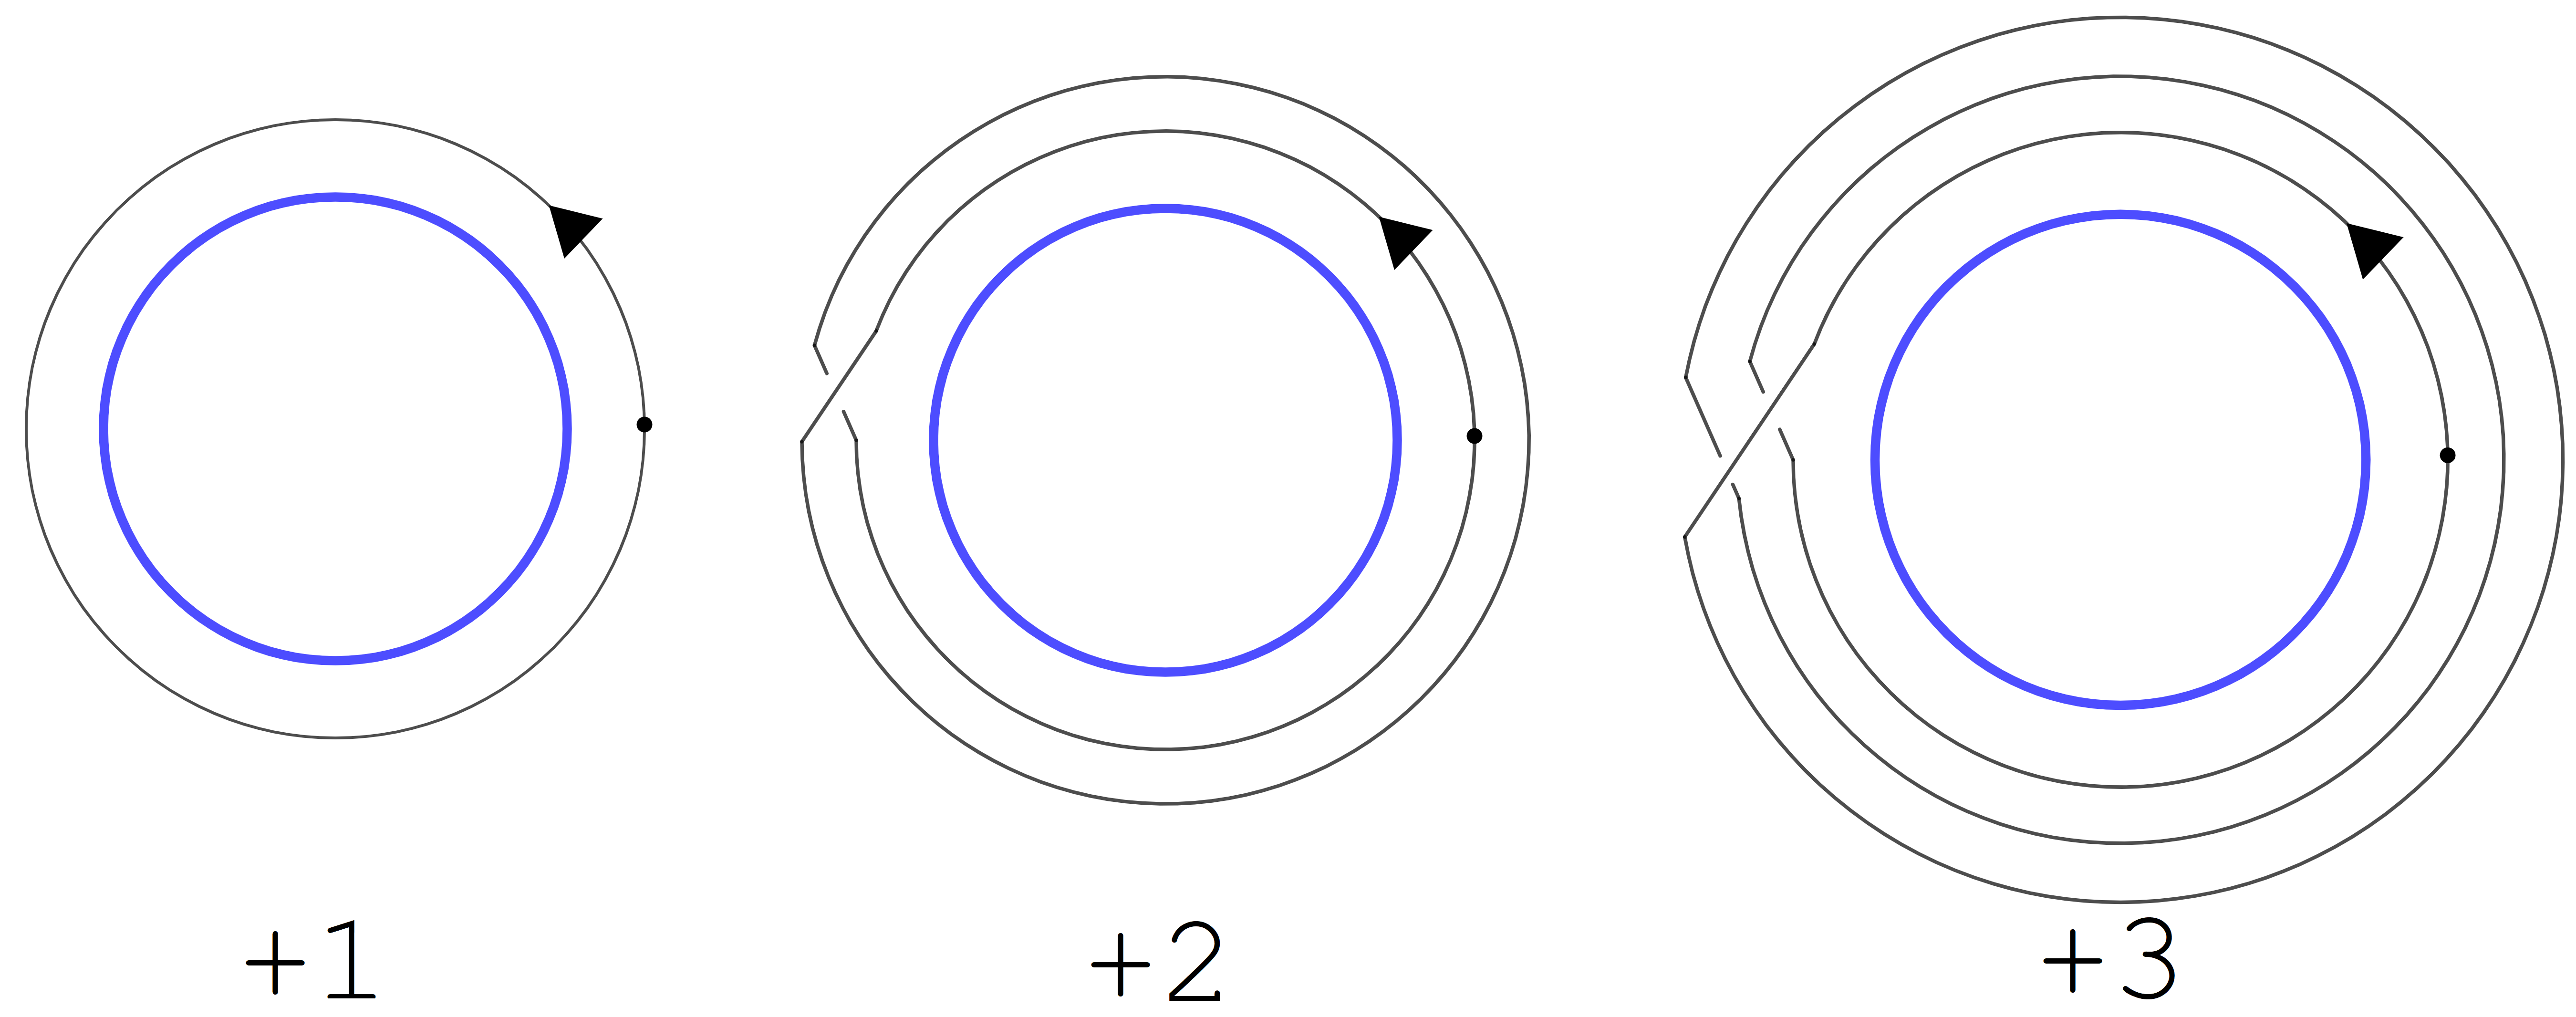
\includegraphics[width= 1\linewidth]{h6.png}
		\caption{\small\textit{\color{duongvaotoanhoc}Hình $6$: Nhóm cơ bản của đường tròn.}}
		\vspace*{-10pt}
	\end{figure}
	Cuối cùng, $f_n \ast f_m \sim f_{n+m}$, phép hợp thành của đường tương thích với phép cộng số nguyên, nghĩa là ta có đẳng cấu nhóm $\pi_1(\mathbb{S}^1) = \mathbb{Z}$.
	\vskip 0.1cm
	\textbf{\color{duongvaotoanhoc}Không gian phủ}
	\begin{figure}[H]
		\vspace*{-5pt}
		\centering
		\captionsetup{labelformat= empty, justification=centering}
		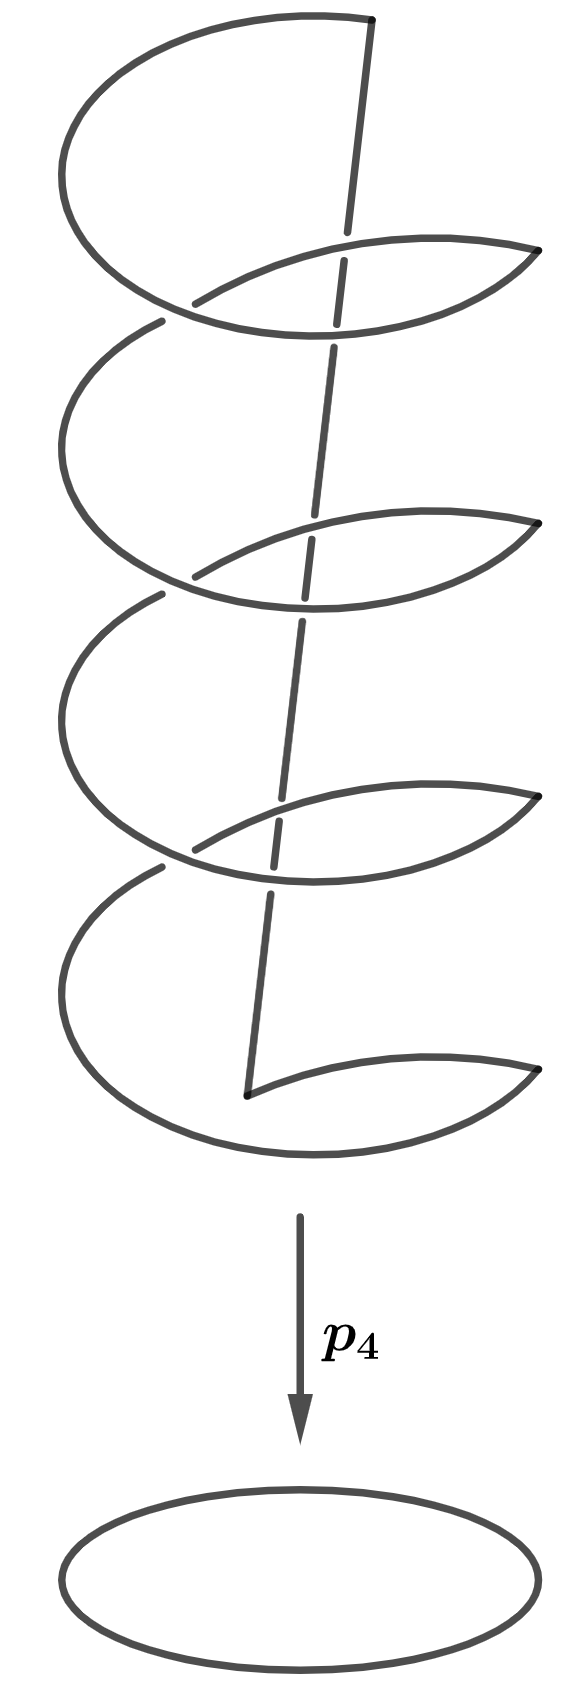
\includegraphics[width= 0.2\linewidth]{h7.png}
		\caption{\small\textit{\color{duongvaotoanhoc}Hình $7$: Đường tròn là một phủ $4$--tờ của chính nó.}}
		\vspace*{-10pt}
	\end{figure}
	Khái niệm gắn liền với nhóm cơ bản là {\bf\color{duongvaotoanhoc} không gian phủ}. Chẳng hạn, cho số nguyên dương $n$ và xét hàm liên tục $p_n: \mathbb{S}^1 \to \mathbb{S}^1$ cho bởi $p_n(z) = z^n$. Với mỗi điểm $w \in \mathbb{S}^1$, các điểm được $p_n$ biến thành $w$ (các căn bậc $n$ của $w$) tạo thành {\bf\color{duongvaotoanhoc} thớ} của $p_n$ tại $w$. Thớ này gồm $n$ điểm rời rạc. Hơn nữa, nếu ta chọn một lân cận $U$ đủ nhỏ quanh $w$ thì thớ của $U$ gồm $n$ thành phần liên thông rời nhau, mỗi thành phần này là một bản sao của U (cụ thể là $p_n$ cảm sinh một phép đồng phôi từ mỗi thành phần này lên $U$). Ta gọi một đó là một {\bf\color{duongvaotoanhoc} phủ $n$--tờ} hay {\bf\color{duongvaotoanhoc} phủ bậc $n$}. 
	\vskip 0.1cm
	Tổng quát, một phủ của không gian tôpô $X$ được cho bởi một không gian tôpô $Y$ cùng một hàm liên tục $p: Y \to X$ (ta coi $X$ là {\bf\color{duongvaotoanhoc} không gian nền} nằm dưới, $Y$ là {\bf\color{duongvaotoanhoc} không gian toàn phần} nằm trên), sao cho mỗi điểm của $X$ đều có một lân cận mà thớ được tạo thành từ một số (có thể vô hạn) bản sao rời rạc. Đây là một điều kiện hoàn toàn địa phương và từ nó không suy ra rằng bản thân $Y$ gồm các bản sao rời rạc của $X$.
		\begin{figure}[H]
		\vspace*{-5pt}
		\centering
		\captionsetup{labelformat= empty, justification=centering}
		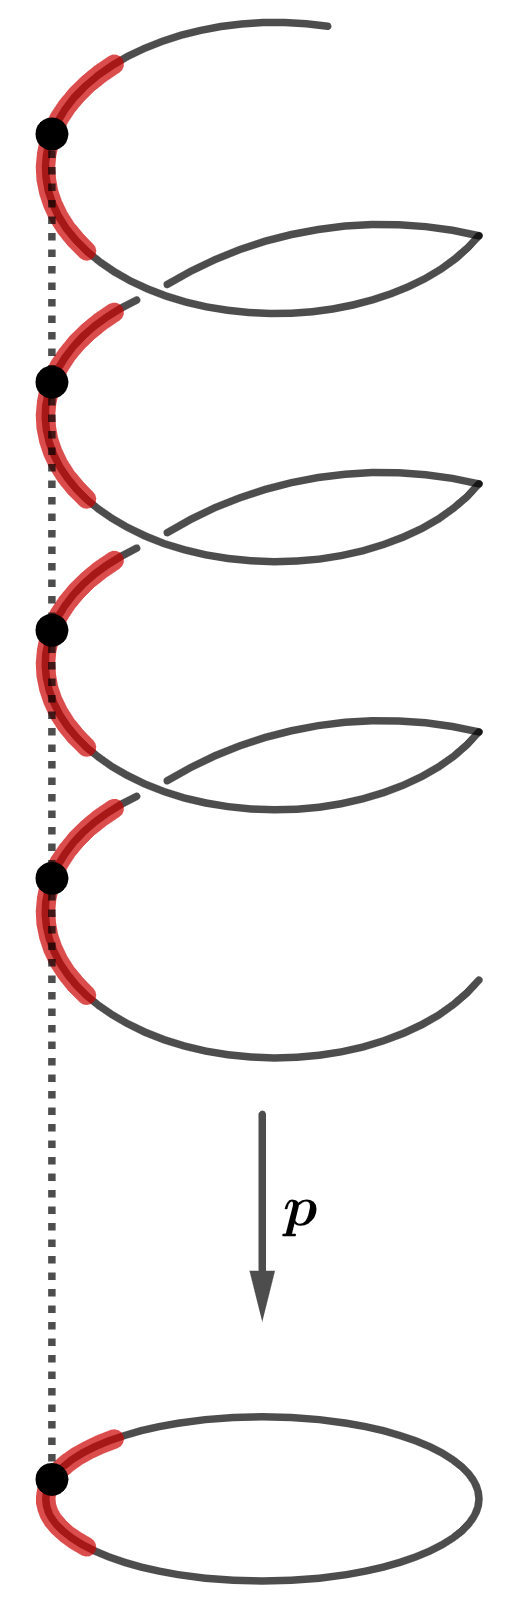
\includegraphics[width= 0.2\linewidth]{h8.png}
		\caption{\small\textit{\color{duongvaotoanhoc}Hình $8$: Phủ phổ dụng của đường tròn, cho bởi phép chiếu đường helix trong không gian $3$--chiều lên mặt phẳng. Mỗi điểm trên đường tròn đều có một lân cận mà thớ được tạo thành từ các bản sao rời rạc của chính lân cận đó.}}
		\vspace*{-5pt}
	\end{figure}
	Một ví dụ về phủ vô hạn tờ là $p: \mathbb{R} \to \mathbb{S}^1$ cho bởi $p(x) = \cos(2\pi x)+i \cdot \sin(2\pi x)$. Phủ này được gọi là {\bf\color{duongvaotoanhoc} phủ phổ dụng} của $\mathbb{S}^1$. Tại sao? Vì thông tin của nhóm cơ bản được thể hiện hoàn toàn trên nó. Một tính chất cơ bản của không gian phủ là tính nâng đường: cho một điểm $z \in \mathbb{S}^1$ và một điểm $x$ trên thớ của $z$, tức là $p(x) = z$. Với một đường bất kỳ $f: I \to \mathbb{S}^1$ xuất phát từ $z$, ta có thể {\bf\color{duongvaotoanhoc} nâng} nó thành một đường {\it duy nhất} $g: I \to \mathbb{R}$ xuất phát từ $x$, nghĩa là $p(g(t)) = f(t)$ và $g(0) = x$. Chẳng hạn khi $f$ là một khuyên tại z (hay $f(0) = f(1) = z$) thì $g(1)$ cũng nằm trên thớ của $z$, điều này tương đương với việc $g(1) - g(0)$ là một số nguyên. Chênh lệch này này hóa ra chính là số vòng quay của khuyên $f$ quanh đường tròn! Đây được gọi là {\bf\color{duongvaotoanhoc} tác động đơn đạo} của nhóm cơ bản $\pi_1(\mathbb{S}^1)$ lên phủ phổ dụng.
	\begin{figure}[H]
		\vspace*{-5pt}
		\centering
		\captionsetup{labelformat= empty, justification=centering}
		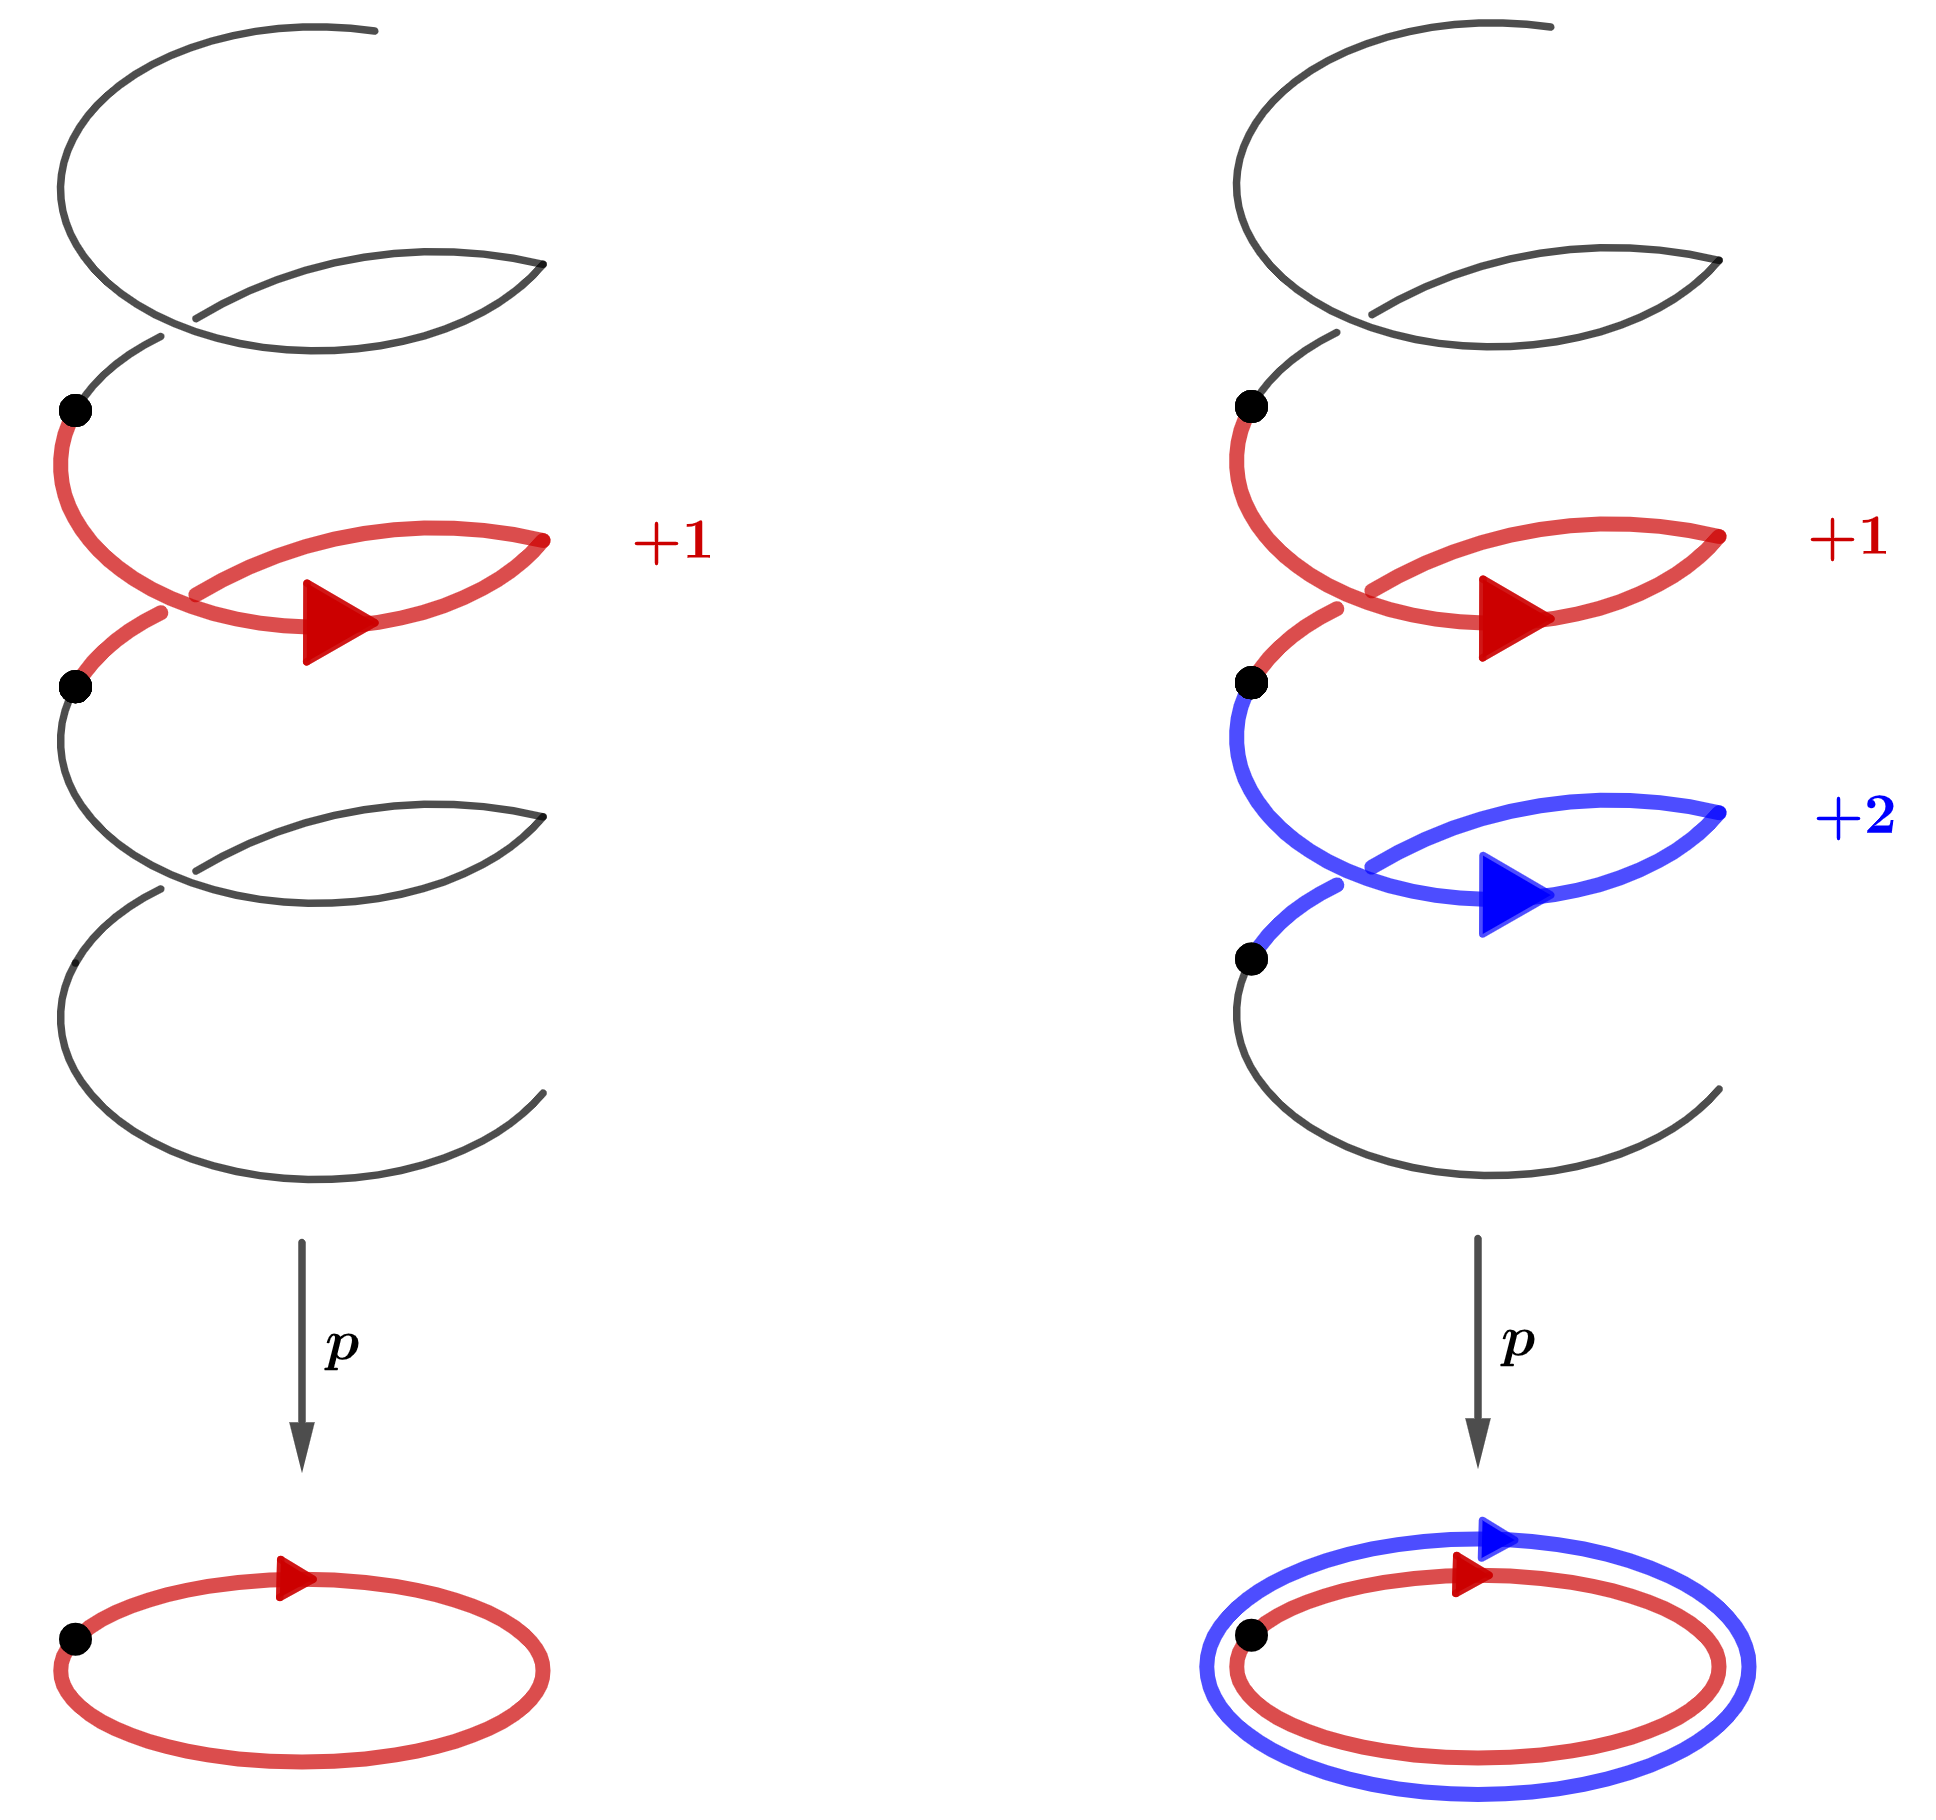
\includegraphics[width= 0.7\linewidth]{h9.png}
		\caption{\small\textit{\color{duongvaotoanhoc}Hình $9$: Tác động đơn đạo của nhóm cơ bản: khuyên $f_2(z) = z^2$ trên đường tròn được nâng thành phép tịnh tiến $g(x) = x+2$ trên phủ phổ dụng.}}
		\vspace*{-10pt}
	\end{figure}
	Như vậy, số vòng quay, vốn là một thông tin bị che mất nếu ta chỉ đơn thuần nhìn vào vết của đường trên không gian nền, đã được phục hồi khi ta nhìn vào không gian phủ.
	\vskip 0.1cm
	Định lý cơ bản của lý thuyết không gian phủ nói rằng có một tương ứng $1-1$ giữa các phủ (sai khác tương đương theo một nghĩa nào đó) với các nhóm con của nhóm cơ bản. Trong trường hợp đường tròn, các nhóm con của $\pi_1(\mathbb{S}^1) = \mathbb{Z}$ gồm $n\mathbb{Z}$ với $n$ nguyên dương (nhóm con các số nguyên chia hết cho $n$), cùng với $\{0\}$. Nhóm $n\mathbb{Z}$ có chỉ số $n$ trong $\mathbb{Z}$ (có $n$ lớp đồng dư modulo $n\mathbb{Z}$), nó ứng với phủ $n$-tờ $p_n: \mathbb{S}^1 \to \mathbb{S}^1$ cho bởi $p_n(z) = z^n$. Nhóm $\{0\}$ ứng với phủ phổ dụng $p: \mathbb{R} \to \mathbb{S}^1$, một phủ vô hạn tờ (và $\{0\}$ cũng có chỉ số vô hạn trong $\mathbb{Z}$). Và đó là tất cả. Nói riêng, với mỗi $n$, vì $\mathbb{Z}$ chỉ có đúng một nhóm con với chỉ số $n$ nên $\mathbb{S}^1$ chỉ có đúng một phủ $n$--tờ (sai khác tương đương).
	\vskip 0.1cm
	\textbf{\color{duongvaotoanhoc}Mở rộng trường}
	\vskip 0.1cm
	Lý thuyết về không gian phủ có một sự tương tự kỳ lạ với lý thuyết mở rộng trường của Galois. Để thấy phiên bản số học của đường tròn $\mathbb{S}^1$, ta quay lại với thế giới đại số. Một {\bf\color{duongvaotoanhoc} trường} là một tập hợp số mà ta có thể làm các phép toán cộng, trừ, nhân, chia. Chính xác hơn, ta có hai phép toán $+$ và $\times$ sao cho chúng thỏa mãn các tiên đề kết hợp, giao hoán, phân phối, có phần tử trung lập $0$, có phần tử đơn vị $1$, mọi ``số'' đều có số đối, và mọi số khác $0$ đều có nghịch đảo. Các ví dụ quen thuộc nhất là $\mathbb{Q}$, $\mathbb{R}$, $\mathbb{C}$. Trong khi đó, $\mathbb{Z}$ không phải một trường vì ta không thể làm phép chia $1 \div 2$ (sao kết quả vẫn nằm trong $\mathbb{Z}$).
	\vskip 0.1cm
	Một thao tác ta có thể làm với các trường là {\bf\color{duongvaotoanhoc} mở rộng}: ta kết nạp thêm nghiệm của một đa thức vô nghiệm trong trường ban đầu, và xét tất cả biểu thức thu được bằng cách cộng, trừ, nhân chia với phần tử mới này. Chẳng hạn, ta biết rằng đa thức $x^2 - 2$ không có nghiệm trong $\mathbb{Q}$. Khi kết nạp số thực $\sqrt{2}$, ta thu được tập các số $a + b\sqrt{2}$ với $a,b \in \mathbb{Q}$. Giá trị tại $\sqrt{2}$ của mọi đa thức hệ số hữu tỷ đều có thể viết được dưới dạng này: ta chỉ cần làm phép chia Euclid cho đa thức $x^2 - 2$ (dư sẽ có dạng $a + bx$) rồi thay $x = \sqrt{2}$. Để làm phép chia cho một số $a+b\sqrt{2} \neq 0$, ta chỉ đơn giản làm phép nhân liên hợp với $a-b\sqrt{2}$, vì $a+b\sqrt{2} = \frac{a^2 - 2b^2}{a-b\sqrt{2}}$. 
	\vskip 0.1cm
	Một câu hỏi mà thoạt nhìn có vẻ lẩm cẩm là ``số $\sqrt{2}$ lấy từ đâu ra?''. Việc xây dựng số thực từ số hữu tỷ là một thao tác phức tạp và nặng tính giải tích (gần như không hề đại số chút nào). Nhưng nếu ta không quan tâm đến tất cả số thực và chỉ muốn ``cái gì đó bình phương lên bằng $2$'' thì sao? Các nhà đại số rất giỏi trong việc này, họ thêm một phần tử mới hoàn toàn hình thức và tuyên bố rằng nó là nghiệm của đa thức $x^2 - 2$, và ký hiệu nó bởi $\sqrt{2}$. Một kiểu ``lý sự cùn'': tôi chẳng quan tâm $\sqrt{2}$ đến từ đâu, tôi chỉ cần biết nó thỏa mãn $(\sqrt{2})^2 - 2$ = 0 và tôi cộng trừ nhân chia với nó cứ như thể chẳng có gì xảy ra vậy! Nếu để ý, ta sẽ thấy rằng một khi ta đã gọi một nghiệm là $\sqrt{2}$ thì nghiệm còn lại của $x^2 - 2$ là $-\sqrt{2}$ (đa thức bậc $2$ nên chỉ có hai nghiệm này). Theo phong cách của các nhà đại số thì hoàn toàn không có cách nào để phân biệt giữa $\sqrt{2}$ và $-\sqrt{2}$ hết. Cứ chỗ nào có $\sqrt{2}$ thì thay bởi $-\sqrt{2}$, các tính toán vẫn không thay đổi. Để phân biệt hai số này, ta cần một thao mới (so với cộng, trừ, nhân, chia) là {\it so sánh}. Biết rằng có có hai căn bậc hai của $2$ trong $\mathbb{R}$, ta sẽ tuyên bố rằng, số nào lớn hơn $0$ thì được gọi là $\sqrt{2}$. Tình trạng tương tự xảy ra khi ta kết nạp vào $\mathbb{R}$ số $i$ và tuyên bố rằng $i^2 + 1 = 0$, thứ mà ngày nay ta gọi là {\bf\color{duongvaotoanhoc} số ảo}. Lúc này, để phân biệt $i$ với $-i$, ta không thể so sánh các số phức được nữa, giải pháp duy nhất là chọn một trong hai căn bậc hai của $-1$ và gọi nó là~$i$.
	\vskip 0.1cm
	Tổng quát hơn, nếu $f$ là một đa thức bất khả quy bậc $n > 1$ với hệ số trong một trường $K$ nào đó thì $f$ không có nghiệm trong $K$ (nếu nó có nghiệm $\alpha \in K$ thì nó chia hết cho đa thức $x - \alpha$, trái với giả thiết bất khả quy). Ta tuyên bố một cách hình thức rằng $\alpha$ là một ``nghiệm nào đó'' của $f$ và kết nạp $\alpha$ vào $K$. Trường mới thu được, ký hiệu bởi $K(\alpha)$, gồm các tổng (hình thức) có dạng $a_0+a_1\alpha+\cdots+a_{n-1}\alpha^{n-1}$, với $a_i \in K$. Ta cộng và trừ chúng một cách hiển nhiên. Khi làm phép nhân, ta chỉ cần chú ý rằng $f(\alpha) = 0$, từ đó $\alpha^n$ cũng có dạng $a_0+a_1\alpha+\cdots+a_{n-1}\alpha^{n-1}$, suy rộng ra thì giá trị tại $\alpha$ của mọi đa thức (bậc tùy ý) với hệ số trong $K$ cũng có dạng này. Để làm phép chia cho một phần tử $a_0+a_1\alpha+\cdots+a_{n-1}\alpha^{n-1} \neq 0$, ta xét đa thức $g(x) a_0+a_1x+\cdots+a_{n-1}x^{n-1}$. Vì $g(x) \neq 0$ nên $g$ không thể chia hết cho $f$, hay $g$ và $f$ nguyên tố cùng nhau (giả thiết $f$ bất khả quy được dùng ở đây), nên thuật toán Bézout cho ta các đa thức $u$, $v$ sao cho $fu+gv=1$, suy ra $g(\alpha)v(\alpha) = 1$, hay $v(\alpha)$ chính là nghịch đảo cần tìm của $g(\alpha)$. Mở rộng trường $K(\alpha)/K$ được gọi là một {\bf\color{duongvaotoanhoc} mở rộng bậc $n$}.
	\vskip 0.1cm
	\textbf{\color{duongvaotoanhoc}Trường hữu hạn}
	\vskip 0.1cm
	Nếu ta xét tập hợp $\mathbb{Z}/n\mathbb{Z}$ các lớp đồng dư modulo $n$ với $n$ là số nguyên dương cho trước, ta có thể làm phép cộng và phép nhân trên chúng một cách hiển nhiên. Thế thì $\mathbb{Z}/n\mathbb{Z}$ là một trường khi và chỉ khi $n = p$ là một số nguyên tố. Ta ký hiệu $\mathbb{Z}/p\mathbb{Z}$ bởi $\mathbb{F}_p$, một trường có $p$ phần tử. Các trường hữu hạn tìm thấy những ứng dụng quan trọng trong lý thuyết bảo mật hiện đại. 
	\vskip 0.1cm
	Tạm gác lại các ứng dụng của $\mathbb{F}_p$ trong tin học, ta hãy xem chúng có liên hệ gì với tôpô. Ta áp dụng phép mở rộng trường cho trường $\mathbb{F}_p$. Một suy luận đếm bằng hàm sinh và công thức nghịch đảo M\"obius đảm bảo rằng với mỗi số nguyên dương $n$, luôn tồn tại một đa thức $f$ với hệ số trong $\mathbb{F}_p$, bậc $n$, và bất khả quy. Kết nạp một nghiệm hình thức $\alpha$ của $f$ vào $\mathbb{F}_p$, ta thu được trường mới mà mỗi phần tử được viết duy nhất dưới dạng dạng $a_0+a_1\alpha+\cdots+a_{n-1}\alpha^{n-1}$, với $a_i \in \mathbb{F}_p$. Trường mới này vì thế có $p^n$ phần tử.
	\vskip 0.1cm
	Chẳng hạn, với $p = n = 2$, đa thức bậc $2$ bất khả quy duy nhất trên $\mathbb{F}_2$ là $x^2+x+1$. Ta tuyên bố rằng $\alpha$ là ``cái gì đó'' sao cho $\alpha^2 + \alpha + 1 = 0$ và kết nạp nó vào $\mathbb{F}_2$. Khi đó ta thu được một trường với $4$ phần tử là $0$, $1$, $\alpha$, $1 + \alpha$. Hai phần tử $\alpha$ và $1 + \alpha$ là nghịch đảo của nhau vì $\alpha(1 + \alpha) = \alpha^2 + \alpha = -1 = 1$ (ta đang xét modulo $2$!), từ đó ta có thể dễ dàng cộng, trừ, nhân, chia trên $4$ phần tử này.
	\vskip 0.1cm
	Trở lại với trường với $p^n$ phần tử, ta đã thấy rằng nó tồn tại. Ta muốn nó ``duy nhất'' theo nghĩa: hai trường có $p^n$ phần tử thì {\bf\color{duongvaotoanhoc} đẳng cấu} với nhau; một đẳng cấu trường là một tương ứng $1-1$ tương thích với các cấu trúc của trường (các phép toán cộng, trừ, nhân, chia, số $0$, số $1$). Trước hết, bằng một suy luận đại số tuyến tính đơn giản, mỗi trường hữu hạn $\mathbb{F}$ đều phải có số phần tử $q$ là lũy thừa của một số nguyên tố, $q = p^n$ chẳng hạn. Lúc này, $\mathbb{F}$ luôn ``chứa'' trường $\mathbb{F}_p$, theo nghĩa các phần tử $0,1,2 \ldots p-1$ trong $\mathbb{F}$ tạo thành một bản sao đẳng cấu với $\mathbb{F}_p$; ta cộng, trừ, nhân, chia chúng theo modulo $p$. Khi bỏ đi số $0$ khỏi $\mathbb{F}$, ta thu được một nhóm đối với phép nhân, một nhóm với $q-1$ phần tử. Định lý Lagrange trong lý thuyết nhóm đảm bảo rằng $a^{q-1} = 1$ với mọi $a \neq 0$, hay $a^q = a$ với mọi $a \in \mathbb{F}$. Đây là một tổng quát hóa của định lý nhỏ Fermat trong $\mathbb{F}_p$ (vì thực ra cách chứng minh cũng y hệt). Vậy, mọi phần tử của $\mathbb{F}$ đều là nghiệm của đa thức $x^q - x$, hay $\mathbb{F}$ thu được bằng cách kết nạp tất cả nghiệm của đa thức này vào $\mathbb{F}_p$. Lý thuyết mở rộng trường gọi $\mathbb{F}$ là (một) {\bf\color{duongvaotoanhoc} trường phân rã} của đa thức $x^q - x$, và nó đảm bảo rằng trường phân rã là duy nhất sai khác đẳng cấu. Như vậy, với mọi lũy thừa nguyên tố $p^n$, có duy nhất một trường với $p^n$ phần tử, một mở rộng bậc $n$ của $\mathbb{F}_p$.
	\vskip 0.1cm
	Tổng quát hơn, nếu $\mathbb{F}$ là một trường hữu hạn thì với mọi số nguyên dương $n$, tồn tại duy nhất (sai khác đẳng cấu) một mở rộng bậc $n$ của $\mathbb{F}$. Ta đã từng nói rằng lý thuyết không gian phủ có sự tương tự với lý thuyết mở rộng trường. Hãy nghĩ về các phủ $n$-tờ như các mở rộng bậc $n$. Vậy chẳng phải trường hữu hạn $\mathbb{F}$ rất giống đường tròn $\mathbb{S}^1$ ư? Dù trông nó như một sự tình cờ, ta hãy miễn cưỡng lấy quan sát này làm mở đầu cho sự liên hệ giữa tôpô và số học ở phần dưới. Sớm thôi, ta sẽ thấy rằng nó cũng không ngẫu nhiên lắm đâu.
	\vskip 0.1cm
	\textbf{\color{duongvaotoanhoc}Lược đồ}
	\vskip 0.1cm
	Bây giờ, hãy dạo qua thế giới hình học đại số một chút. Với ý tưởng tiên phong của Descartes là nghiên cứu các đối tượng hình học bằng các hệ tọa độ và phương trình đa thức, người ta đã dần dần phát triển hình học đại số. Khác với những người bạn bên tôpô học, các nhà hình học đại số nghiên cứu các đối tượng cứng nhắc hơn: tập nghiệm của các hệ phương trình đa thức. Sau một thời gian, giới toán học nhận ra rằng các trực giác hình học thường mang đến các chứng minh không chặt chẽ và đặc biệt là không giúp gì được ở số chiều cao hơn. Họ đã chuyển sang dùng đại số giao hoán làm công cụ chính để nghiên cứu hình học. Grothendieck, nhà toán học được công nhận rộng rãi là có ảnh hưởng nhất thế kỷ XX, đã cách mạng hóa hình học đại số một lần nữa bằng định nghĩa {\bf\color{duongvaotoanhoc} lược đồ}.
	\vskip 0.1cm
	Ta quay lại với khái niệm trường. Nếu bỏ qua việc luôn làm được phép chia, ta thu được khái niệm {\bf\color{duongvaotoanhoc} vành}. Chẳng hạn, $\mathbb{Z}$ và $\mathbb{Z}/n\mathbb{Z}$ là các vành (phép cộng và phép nhân được hiểu theo nghĩa hiển nhiên). Chú ý rằng ta vẫn yêu cầu làm được phép trừ, nên $\mathbb{N}$ không phải là một vành. Với mỗi vành $R$, ta xây dựng được một không gian tôpô $\text{Spec}(R)$, được gọi là {\bf\color{duongvaotoanhoc} phổ} của $R$. Nếu chỉ nhìn $\text{Spec}(R)$ như một không gian thì ta mất rất nhiều thông tin. Chẳng hạn, phổ của một trường luôn là một điểm. Vì thế, người ta đã làm giàu $\text{Spec}(R)$ một cấu trúc gọi là {\bf\color{duongvaotoanhoc} bó}, chúng làm cho $\text{Spec}(R)$ trở thành một lược đồ.
	\vskip 0.1cm
	Cũng như việc người ta quan tâm đến các hàm liên tục giữa các không gian tôpô, trong hình học đại số người ta quan tâm đến các {\bf\color{duongvaotoanhoc} cấu xạ} giữa các lược đồ. Một cấu xạ $\text{Spec}(R) \to \text{Spec}(S)$ đơn giản được cho bởi một {\bf\color{duongvaotoanhoc} đồng cấu vành} theo chiều ngược lại $f: S \to R$, đồng cấu ở đây nghĩa là $f(x+y) = f(x)+f(y)$, $f(xy) = f(x)f(y)$ và $f(1) = 1$. Chẳng hạn, $\mathbb{Z}$ là một vành con của $\mathbb{Q}$, và phép bao hàm $\mathbb{Z} \to \mathbb{Q}$ cho ta một cấu xạ $\text{Spec}(\mathbb{Q}) \to \text{Spec}(\mathbb{Z})$. Về mặt tôpô thì $\text{Spec}(\mathbb{Q})$ chỉ có một điểm, nên ảnh của cấu xạ này là một điểm của $\text{Spec}(\mathbb{Z})$, được gọi là {\bf\color{duongvaotoanhoc} điểm tổng quát}. Với mỗi số nguyên tố $p$, phép lấy dư modulo $p: \mathbb{Z} \to \mathbb{F}_p$ cho ta một cấu xạ $\text{Spec}(\mathbb{F}_p) \to \text{Spec}(\mathbb{Z})$, đó là một {\bf\color{duongvaotoanhoc} điểm đóng}. Các điểm đóng này và điểm tổng quát tạo nên không gian $\text{Spec}(\mathbb{Z})$. Khác với các không gian Euclid, tôpô trên lược đồ $\text{Spec}(\mathbb{Z})$ rất thô: điểm tổng quát là một điểm nhưng lại trù mật trong cả không gian (người ta hay nói ``điểm tổng quát là điểm nằm ở mọi nơi, nhưng không nằm cụ thể ở đâu cả'').
	\vskip 0.1cm
	Quay lại với lý thuyết không gian phủ. Khi áp dụng nó cho lược đồ, ta không thể chỉ xét khía cạnh tôpô ngây thơ được. Ta muốn $\text{Spec}(\mathbb{F}_p)$ giống với đường tròn $\mathbb{S}^1$, nhưng $\text{Spec}(\mathbb{F}_p)$ lại chỉ có một điểm. Vấn đề với không gian tôpô $\text{Spec}(R)$ là nó có quá ít lân cận, mỗi lân cận đều quá lớn. Cách khắc phục là sáng tạo ra một khái niệm tôpô mới dùng được cho các lược đồ (thứ mà ngày nay gọi là tôpô Grothendieck), với các ``lân cận'' mới. Một trong những loại tôpô đủ mạnh để phân biệt các ``không gian 1 điểm'' $\text{Spec}(K)$ (với $K$ là các trường) là {\bf\color{duongvaotoanhoc} tôpô étale}. Từ ``étale'' được lấy từ văn học Pháp, mang nghĩa nôm na là trạng thái dịu dàng của biển. Với công cụ mới này, người ta định nghĩa được khái niệm nhóm cơ bản étale của lược đồ. Chẳng hạn, nhóm cơ bản étale của $\text{Spec}(\mathbb{F}_p)$ là một nhóm có cùng họ hàng với $\mathbb{Z}$, gọi là ``$\mathbb{Z}$ mũ''. Điều này giải thích vì sao việc coi $\text{Spec}(\mathbb{F}_p)$ như đường tròn $\mathbb{S}^1$ là hợp lý. Tương tự, khái niệm phủ trong thế giới lược đồ phải được hiểu là phủ étale. Đối với các trường, một phủ étale của $\text{Spec}(K)$ đơn giản là $\text{Spec}(L)$, với $L/K$ là một mở rộng bậc hữu hạn. Như vậy, dù $\text{Spec}(K)$ về mặt tôpô chỉ một $1$ điểm, nó lại có nhóm cơ bản étale không tầm thường, hay có rất nhiều phủ. 
	\vskip 0.1cm
	Thực ra khái niệm mở rộng trường và mở rộng vành còn cho ta thêm một chút bên phía tôpô, nó ứng với khái niệm {\bf\color{duongvaotoanhoc} phủ phân nhánh}. Nói nôm na, một phủ phân nhánh bậc $n$ là một hàm liên tục $p: Y \to X$ sao cho nếu bỏ đi một số hữu hạn điểm của $X$ (và các điểm của $Y$ nằm trên chúng) thì ta thu được một phủ $n$-tờ. Các điểm bỏ đi kia (cùng các điểm nằm trên) gọi là các {\bf\color{duongvaotoanhoc} điểm rẽ nhánh} của $p$. Hiện tượng rẽ nhánh là phiên bản hình học của hiện tượng ``nghiệm bội'' trong đại số. Ta xét ví dụ khi $Y$ là đường cong elliptic cho bởi phương trình $y^2=x(x-1)(x-2)$ trong $\mathbb{C}^2$ và $X = \mathbb{C}$. Lấy $p$ là phép chiếu lên trục hoành, $p(x,y) = x$. Khi bỏ đi các điểm $0, 1, 2$ khỏi $X$ (và các điểm $(0,0), (1,0), (2,0)$ khỏi $Y$), ta thu được một phủ $2$--tờ: với mỗi $x \neq 0,1,2$ thì phương trình $y^2=x(x-1)(x-2)$ có hai nghiệm phức phân biệt. Ở các điểm $0, 1, 2$ xảy ra hiện tượng rẽ nhánh, phương trình $y^2=0$ có nghiệm kép $y=0$. Ta nói rằng {\bf\color{duongvaotoanhoc} chỉ số rẽ nhánh} của $p$ tại các điểm $(0,0)$, $(1,0)$, $(2,0)$ bằng $2$.
	\vskip 0.1cm
	\textbf{\color{duongvaotoanhoc}Lý thuyết số đại số}
	\vskip 0.1cm
	Để tìm hiểu các phủ (étale) phân nhánh của lược đồ $\text{Spec}(\mathbb{Z})$, ta bắt đầu từ điểm tổng quát: Phủ étale của $\text{Spec}(\mathbb{Q})$ thì có dạng $\text{Spec}(K)$, với $K = \mathbb{Q}(\alpha)$, và $\alpha$ là nghiệm của một đa thức bậc $n$ bất khả quy với hệ số hữu tỷ. Số $\alpha$ như vậy được gọi là một {\bf\color{duongvaotoanhoc} số đại số}, chẳng hạn $\sqrt{2}, \sqrt[3]{2}, \frac{1 + \sqrt{-3}}{2}$ là các số đại số. Trường $K$ được gọi là một {\bf\color{duongvaotoanhoc} trường số}, và mọi phần tử của nó đều là số đại số. Ta muốn thứ gì đó trong $K$ đóng vai trò như các số nguyên đối với số hữu tỷ. Đó là các {\bf\color{duongvaotoanhoc} số nguyên đại số}. Chúng là những phần tử của $K$ mà là nghiệm của một đa thức với hệ số nguyên và hệ số đầu bằng $1$. Chẳng hạn $\sqrt{2}$ là một số đại số vì nó là nghiệm của $x^2 - 2$. $\frac{1 + \sqrt{5}}{2}$ cũng là một số nguyên đại số (dù trông không có vẻ vậy) vì nó là nghiệm của $x^2-x-1$. Các số nguyên đại số trong $K$ tạo thành một vành $\mathcal{O}$. Việc chuyển từ $\mathbb{Z}$ sang $\mathcal{O}$ là chuyển từ lý thuyết số sơ cấp sang lý thuyết số đại số. Một bài tập đơn giản (bằng cách dùng phân tích duy nhất ra thừa số nguyên tố) là: Các số nguyên đại số trong $\mathbb{Q}$ chính là các số nguyên theo nghĩa cổ điển.
	\vskip 0.1cm
	Lý thuyết số đại số xuất phát từ nỗ lực chứng minh định lý lớn Fermat của Cauchy, Lamé... Ý tưởng như sau: với phương trình $x^2 + y^2 = z^2$ chẳng hạn, ta giải bằng cách đưa về $x^2=z^2-y^2=(z-y)(z+y)$, sau đó lập luận (với phân tích duy nhất ra thừa số nguyên tố) rằng $z-y$ và $z+y$ phải là các số chính phương. Bây giờ, xét phương trình $x^p+y^p=z^p$, với p là số nguyên tố lẻ (dễ thấy ta chỉ cần xét trường hợp này). Để phân tích triệt để $z^p-y^p$ thành các nhân tử bậc nhất, ta buộc phải dùng căn bậc $p$ phức của $1$. Gọi nó là $\zeta = \cos(\frac{2\pi}{p})+i \cdot \sin(\frac{2\pi}{p})$. Thế thì $\zeta$ là một số nguyên đại số (nghiệm của phương trình $x^p - 1$). Và như vậy ta đưa về chứng minh rằng phương trình trên không có nghiệm trong vành mới $\mathbb{Z}[\zeta]$, vành các số nguyên đại số của $\mathbb{Q}(\zeta)$. Sơ hở của cách tiếp cận này là lập luận như trong trường hợp $p=2$ không còn đúng nữa, vì nói chung không có phân tích duy nhất ra thừa số nguyên tố trong $\mathbb{Z}[\zeta]$.
	\vskip 0.1cm
	Một ví dụ về sự thiếu sốt của phân tích duy nhất là trường số $K = \mathbb{Q}(\sqrt{-5})$. Vành số nguyên đại số của nó là $\mathcal{O} = \mathbb{Z}[\sqrt{-5}]$, gồm các số có dạng $a+b\sqrt{-5}$ với $a,b \in \mathbb{Z}$. Số $6$ có thể phân tích thành $6 = 2 \cdot 3 = (1+\sqrt{-5}) \cdot (-\sqrt{-5})$. Để thấy rằng hai phân tích này là triệt để và thực sự khác nhau, ta định nghĩa {\bf\color{duongvaotoanhoc} chuẩn} của một số $a+b\sqrt{-5}$ bởi $N(a+b\sqrt{-5}) = a^2 + 5b^2$. Đây là một số tự nhiên, và ta thấy ngay rằng $N(xy) = N(x)N(y)$. Trong phân tích $6 = 2 \cdot 3 = (1+\sqrt{-5}) \cdot (-\sqrt{-5})$, ta có $N(2) = 4, N(3) = 9, N(1+\sqrt{-5}) = N(1-\sqrt{-5}) = 6$, nên các nhân tử xuất hiện ở hai phân tích thực sự khác nhau.  Ngoài ra, về cơ bản ta không thể phân tích thêm được nữa, vì không có phần tử nào có chuẩn bằng $2$ hoặc $3$ (một tính toán số học đơn giản cho thấy rằng phương trình các $a^2 + 5b^2 = 2$ và $a^2 + 5b^2 = 3$ đều không có nghiệm nguyên). Điều này cho thấy sự thiếu sót của phân tích duy nhất ra thừa số nguyên tố trong $\mathbb{Z}[\sqrt{-5}]$.
	\vskip 0.1cm
	Sự sụp đổ của phân tích duy nhất trong $\mathcal{O}$ đã chấm dứt hi vọng chứng minh định lý lớn Fermat bằng lý thuyết số đại số cổ điển. Dù vậy, vành $\mathcal{O}$ vẫn giữ được một tính chất của vành $\mathbb{Z}$; nó là một {\bf\color{duongvaotoanhoc} vành Dedekind}. Thay vì phân tích duy nhất của các số, người ta định nghĩa khái niệm {\bf\color{duongvaotoanhoc} số lý tưởng} (cái mà ngày nay gọi là {\bf\color{duongvaotoanhoc} iđêan}). Đại khái nó là thứ gì đó cho phép nói về quan hệ chia hết cũng như làm phép nhân. Việc $\mathcal{O}$ là vành Dedekind có nghĩa là mọi số lý tưởng đều phân tích một cách duy nhất ra các số lý tưởng nguyên tố. Một số nguyên đại số $a \in \mathcal{O}$ định nghĩa một số lý tưởng $(a)$, được gọi là một số lý tưởng chính. Hai số $a$ và $b$ định nghĩa cùng một số lý tưởng nếu chúng {\bf\color{duongvaotoanhoc} liên kết}, nghĩa là $a|b$ đồng thời $b|a$. Nói riêng, nếu là $u|1$ thì $(u) = (1)$. Nếu tất cả số lý tưởng nguyên tố đều có dạng trên thì $\mathcal{O}$ có phân tích duy nhất của các số (thực sự). Điều này không đúng trong $\mathbb{Z}[\sqrt{-5}]$; cụ thể là khi phân tích $(6) = (2) \cdot (3) = (1 + \sqrt{-5}) \cdot (1 - \sqrt{-5})$, ta vẫn phân tích được tiếp: $(2) = \mathfrak{p}_1\mathfrak{p}_2$, $(3) = \mathfrak{p}_3\mathfrak{p}_4$, $(1 + \sqrt{-5}) = \mathfrak{p}_1\mathfrak{p}_3$, $(1 - \sqrt{-5}) = \mathfrak{p}_2\mathfrak{p}_4$, trong đó $\mathfrak{p}_1, \mathfrak{p}_2, \mathfrak{p}_3, \mathfrak{p}_4$ là các số lý tưởng nguyên tố {\it không chính}. Chuẩn của chúng lần lượt là $N(\mathfrak{p}_1) = N(\mathfrak{p}_2) = 2$ và $N(\mathfrak{p}_3) = N(\mathfrak{p}_4) = 3$. Như vậy ta có phân tích duy nhất của $(6)$ thành các số lý tưởng.
	\vskip 0.1cm
	Cũng như mỗi số nguyên tố $p$ ứng với các điểm đóng $\text{Spec}(\mathbb{F}_p) \to \text{Spec}(\mathbb{Z})$, mỗi số lý tưởng nguyên tố $\mathfrak{p}$ trong trong $\mathcal{O}$ cho ta một trường hữu hạn $\mathbb{F}_{\mathfrak{p}}$ (gọi là {\bf\color{duongvaotoanhoc} trường thặng dư} của $\mathfrak{p}$), cùng một điểm đóng $\text{Spec}(\mathbb{F}_{\mathfrak{p}}) \to \text{Spec}(\mathcal{O})$. Cùng với điểm tổng quát $\text{Spec}(K)$, chúng tạo thành lược đồ $\text{Spec}(\mathcal{O})$. Vì $\mathbb{Z}$ là một vành con của $\mathcal{O}$, ta có một cấu xạ $\text{Spec}(\mathcal{O}) \to \text{Spec}(\mathbb{Z})$, một phủ étale phân nhánh. Mỗi số nguyên tố $p$ trong $\mathbb{Z}$ có thể không còn là số lý tưởng nguyên tố trong $\mathbb{O}$, nó phân rã thành tích của một số hữu hạn số lý tưởng nguyên tố, $(p) = \mathfrak{p_1}\mathfrak{p_2}\cdots\mathfrak{p_n}$. Các số lý tưởng nguyên tố xuất hiện trong phân tích trên chính xác là những điểm của $\text{Spec}(\mathcal{O})$ nằm trên điểm đóng của $\text{Spec}(\mathbb{Z})$ ứng với $p$. Hiện tượng phân nhánh nhánh xảy ra nếu có một số lý tưởng $\mathfrak{p}_i$ xuất hiện nhiều lần trong phân tích trên, ta gọi đó số lần đó là {\bf\color{duongvaotoanhoc} chỉ số rẽ nhánh} của $\mathfrak{p}_i$, nó đóng vai trò như chỉ số rẽ nhánh trong tôpô cổ điển.
	\vskip 0.1cm
	Một bất đẳng thức trong lý thuyết số đại số, {\it chặn Minkowski}, cho phép xác định cụ thể phân tích trên. Hơn thế nữa, nó còn cho ta biết chính xác khi nào thì một số nguyên tố $p$ rẽ nhánh trong $\mathcal{O}$. Một hệ quả của nó là với mọi trường số $K$, luôn có ít nhất một số nguyên tố $p$ rẽ nhánh trong vành $\mathcal{O}$ các số nguyên đại số trong $K$, nghĩa là $\text{Spec}(\mathbb{Z})$ không có phủ  étale không rẽ nhánh nào ngoài phủ tầm thường (cho bởi ánh xạ đồng nhất $\mathbb{Z} \to \mathbb{Z}$), hay nó là đơn liên.
	\vskip 0.1cm
	\textbf{\color{duongvaotoanhoc}Nút}
	\vskip 0.1cm
	Trong thế giới của các không gian tôpô thì có rất nhiều không gian đơn liên, và ta muốn tìm cái nào giống với $\text{Spec}(\mathbb{Z})$. Sự đột phá nằm ở các phát hiện sau đây của Mumford, Manin, và sau này là Mazur. Ở phía tôpô, các khái niệm điểm ($0$--chiều), đường ($1$--chiều), mặt ($2$--chiều) được tổng quát lên thành các đa tạp. Một đa tạp $3$--chiều là một không gian tôpô mà nhìn địa phương thì giống như không gian Euclid $\mathbb{R}^3$ (cũng như bề mặt trái đất là một đa tạp $2$--chiều, nhìn địa phương thì giống như mặt phẳng).
	\vskip 0.1cm
	Bên cạnh nhóm cơ bản, tôpô đại số cổ điển còn cung cấp các bất biến đại số khác cho các không gian tôpô, gọi là các {\bf\color{duongvaotoanhoc} nhóm đồng điều}. Nhóm đồng điều bậc $n$ của một đa tạp $X$ được xây dựng như sau: Xét các tổ hợp tạo thành từ một số đa tạp con $n$--chiều (chúng được gọi là các {\bf\color{duongvaotoanhoc} $n$-dây chuyền}). Nếu chúng tạo thành một vòng kín, ta gọi nó là một {\bf\color{duongvaotoanhoc} $n$--chu trình}. Nếu nó tạo thành biên của một đa tạp con $(n+1)$--chiều, ta gọi nó là một {\bf\color{duongvaotoanhoc} $n$--biên}. Một $n$--biên thì luôn là một $n$--chu trình. Nhóm $H_n(X)$ được định nghĩa là chênh lệch giữa các nhóm các $n$--chu trình và nhóm các $n$--biên: một $n$--chu trình mà không phải $n$--biên thì nó bao quanh một ``lỗ thủng'' $(n+1)$--chiều; như vậy các nhóm đồng điều phát hiện các lỗ thủng trên $X$. Phiên bản đối ngẫu của đồng điều là {\bf\color{duongvaotoanhoc} đối đồng điều}, các nhóm $H^n(X)$. Về cơ bản thì chúng cũng phát hiện các lỗ thủng. Về mặt kỹ thuật thì chúng dễ tính toán hơn đồng điều một chút, đồng thời có nhiều cấu trúc hơn. {\it Đối ngẫu Poincaré} nói rằng nếu $X$ là một đa tạp đóng, khả định hướng, $d$--chiều, thì ta có một đối ngẫu hoàn hảo giữa hai nhóm $H^{d-i}(X)$ và $H^i(X)$ với mỗi $i = 0,1,\ldots,d$.
	\vskip 0.1cm
	Với các lược đồ, các nhóm đối đồng điều nhìn chung không cho thông tin gì (phần lớn chúng bằng $0$) khi ta tính theo tôpô thông thường. Một lần nữa nhờ công của Grothendieck, ta có thể tính đối {\bf\color{duongvaotoanhoc} đồng điều étale}.  Trên một trường, chúng được gọi là đối {\bf\color{duongvaotoanhoc} đồng điều Galois}, một công cụ đã được dùng từ lâu trước đó trong số học. Với các trường hữu hạn, đối đồng điều Galois của chúng rất đơn giản, chúng khác $0$ ngoài bậc $0$ và $1$, và ta có một đối ngẫu hoàn hảo giữa các nhóm đối đồng điều ở hai bậc này. Điều này tương tự với đối ngẫu Poincaré cho các đa tạp $1$--chiều, khẳng định thêm niềm tin rằng phổ của trường hữu hạn là phiên bản đại số của đường tròn. 
	\vskip 0.1cm
	Đối với các lược đồ $\text{Spec}(\mathcal{O})$, với $\mathcal{O}$ là vành số nguyên đại số của một trường số $K$ nào đó, các nhóm đối đồng điều étale thỏa mãn đối ngẫu giữa bậc $0$ và bậc $3$ cũng như bậc $1$ và bậc $2$. Các kết quả này được gọi là {\it đối ngẫu Artin--Verdier}, được khám phá khi áp dụng đối đồng điều étale cho lý thuyết trường các lớp toàn cục, một phần của lý thuyết số. Điều này gợi cho ta rằng phiên bản tôpô của $\text{Spec}(\mathcal{O})$ ``nên" là các đa tạp $3$--chiều. Vậy $\text{Spec}(\mathbb{Z})$ ứng với đa đạp đóng $3$--chiều nào? Ta thấy ở trên rằng $\text{Spec}(\mathbb{Z})$ đơn liên, và đa tạp đóng $3$--chiều đơn liên thì chỉ có thể đồng phôi với mặt (siêu) cầu  $\mathbb{S}^3$! Đó là nội dung của {\it giả thuyết Poincaré}, bài toán duy nhất đã được giải trong $7$ bài toán thiên niên kỷ. Tác giả của lời giải, thiên tài lập dị Perelman, đã từ chối cả Huy chương Fields lẫn Giải Breakthrough cho công trình vô song của mình.
	\vskip 0.1cm
	Sau khi bỏ ra rất nhiều công sức, ta đã thấy được cầu nối mong manh giữa tôpô, rằng phiên bản số học của $\mathbb{S}^1$ là (phổ của) một trường hữu hạn, và của một đa tạp đóng $3$--chiều là vành các số nguyên đại số của một trường số. Bây giờ là lúc chúng ta thu hoạch kết quả, chiêm ngưỡng những sự tương tự đáng ngạc nhiên dựa trên cầu nối này. Một số lý tưởng nguyên tố $\mathfrak{p}$ trong $\mathcal{O}$ cho ta một phép nhúng $\text{Spec}(\mathbb{F}_\mathfrak{p}) \hookrightarrow \text{Spec}(\mathcal{O})$. Về phía tôpô, ta xét các phép nhúng $\mathbb{S}^1 \hookrightarrow M$, với $M$ là một đa tạp (đóng, khả định hướng) $3$-chiều. Chúng được gọi là các {\bf\color{duongvaotoanhoc} nút} trong $M$. Nói riêng, phiên bản tôpô của mỗi số nguyên tố $p$ (với phép nhúng tương ứng $\text{Spec}(\mathbb{F}_p) \hookrightarrow \text{Spec}(\mathbb{Z})$) là một nút trong $\mathbb{S}^3$ (ta sẽ tập trung vào các nút này). Từ một định lý sâu sắc trong tôpô học, {\it định lý Borsuk--Ulam}, ta có thể chỉ ra rằng một phép nhúng như thế không thể là toàn ánh, nghĩa là ta có thể xem một nút như một phép nhúng từ $\mathbb{S}^1$ vào $\mathbb{S}^3$ bỏ đi một điểm, nói cách khác chính là không gian Euclid $\mathbb{R}^3$.
	\vskip 0.1cm
	Để biểu diễn một nút $K: \mathbb{S}^1 \hookrightarrow \mathbb{R}^3$ ta có thể chiếu nó lên một mặt phẳng sau cho tại mỗi điểm giao nhau chỉ có đúng $2$ đường đi qua. Chúng ứng với một {\bf\color{duongvaotoanhoc} sợi trên} và một {\bf\color{duongvaotoanhoc} sợi dưới}, ta biểu diễn sợi dưới bằng nét đứt tại giao điểm đó.  Đó là một {\bf\color{duongvaotoanhoc} biểu đồ phẳng} của nút.
	\begin{figure}[H]
		\vspace*{-5pt}
		\centering
		\captionsetup{labelformat= empty, justification=centering}
		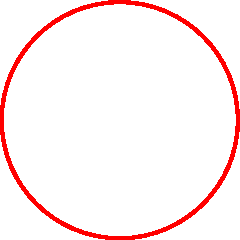
\includegraphics[width= 0.28\linewidth]{unknot.pdf}\quad
		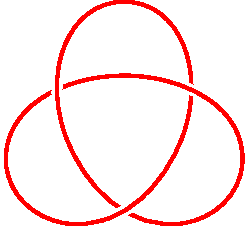
\includegraphics[width= 0.28\linewidth]{trefoil.pdf}\quad
		
\includegraphics[width= 0.28\linewidth]{figure 8.pdf}
		\caption{\small\textit{\color{duongvaotoanhoc}Hình $10$: Biểu đồ phẳng của nút tầm thường, nút ba lá, và nút số $8$.}}
		\vspace*{-10pt}
	\end{figure}
	Tất nhiên, mọi nút đều đồng phôi với $\mathbb{S}^1$. Ta cần cả thông tin về phép nhúng $\mathbb{S}^1 \to \mathbb{R}^3$ để phân biệt các nút với nhau. Các nhà lý thuyết nút gọi sự giống nhau của các nút là {\bf\color{duongvaotoanhoc} đẳng luân}. Một cách trực giác, hai nút đẳng luân nếu ta có thể tháo dỡ một nút rồi buộc thành nút còn lại (mà không cắt được cắt nút ra). Hóa ra, hai nút đẳng luân khi và chỉ khi phần bù của chúng trong $\mathbb{S}^3$ đồng phôi với nhau ({\it định lý Gordon--Luecke}).
	\vskip 0.1cm
	\textbf{\color{duongvaotoanhoc}Từ điển M$^2$KR}
	\vskip 0.1cm
	Từ điển Mazur--Morishita--Kapranov--Reznikov (M$^2$KR) là một danh sách những sự tương tự giữa lý thuyết số và hình học của các đa tạp $3$--chiều; ở đó các số lý tưởng tưởng ứng với các liên kết, các số lý tưởng nguyên tố ứng với các nút. Sau đây là một số tương ứng giữa tôpô và số học trong từ điển này.
	\vskip 0.1cm
	Mỗi số lý tưởng trong $\mathcal{O}$ phân tích thành tích của các số lý tưởng nguyên tố. Phiên bản tôpô của số lý tưởng là {\bf\color{duongvaotoanhoc} liên kết}: một liên kết trong một đa tạp đóng $3$--chiều $M$ là một phép nhúng từ một số hữu hạn bản sao rời rạc của $\mathbb{S}^1$ vào $M$. Các ví dụ về liên kết trong $\mathbb{S}^3$ là {\bf\color{duongvaotoanhoc} liên kết Hopf} và {\bf\color{duongvaotoanhoc} vòng Borromean}, lần lượt được tạo bởi $2$ và $3$ nút tầm thường lồng nhau.
	\begin{figure}[H]
		\vspace*{-15pt}
		\centering
		\captionsetup{labelformat= empty, justification=centering}
		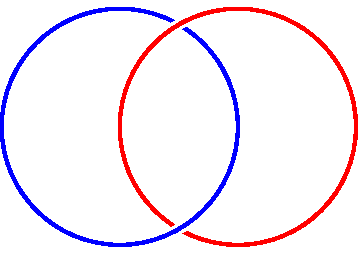
\includegraphics[width= 0.4\linewidth]{hopf.pdf}\quad\quad
		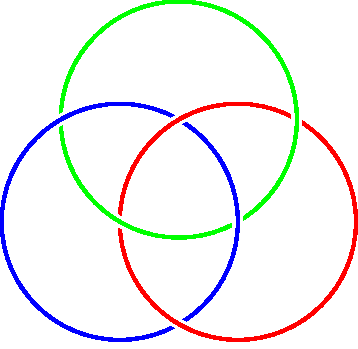
\includegraphics[width= 0.4\linewidth]{borromean.pdf}
		\caption{\small\textit{\color{duongvaotoanhoc}Hình $11$: Biểu đồ phẳng của liên kết Hopf và vòng Borromean.}}
		\vspace*{-10pt}
	\end{figure}
	Để thêm phần thuyết phục rằng tại sao $M$ lại tương ứng với (vành số nguyên đại số) một trường số, ta nhắc đến {\it định lý Alexander}: Mọi đa tạp đóng $3$--chiều đều là một phủ phân nhánh của $\mathbb{S}^3$, trong đó các điểm rẽ nhánh trong $\mathbb{S}^3$ tạo thành một liên kết. Tương tự, một mở rộng $L/K$ của trường số có thể được coi như một phủ phân nhánh giữa hai đa tạp đóng $3$--chiều.
	\vskip 0.1cm
	Một số nguyên đại số $a \in \mathcal{O}$ ứng với một mặt compact $S$ (có thể có biên) nhúng trong đa tạp đóng $3$--chiều $M$. Số lý tưởng chính $(a)$ ứng với biên $\partial S$, đây là một liên kết, và chúng ứng với các $1$--đối biên, tức là phần tử $0$ trong nhóm đồng điều $H_1(M)$. Các số lý tưởng khác tương ứng với các liên kết, chúng là các $1$--chu trình mà không phải biên, đại diện cho các phần tử không tầm thường của $H_1(M)$. Ta biết rằng trong $\mathbb{Z}$ có phân tích duy nhất ra thừa số nguyên tố, hay mọi số lý tưởng nguyên tố đều là số lý tưởng chính. Tương ứng, với $M = \mathbb{S}^3$, ta có $H_1(M) = 0$ (vì $\mathbb{S}^3$ không có lỗ thủng $2$--chiều nào), nghĩa là mọi liên kết đều là biên của một mặt nào đó. Seifert đã đưa ra một thuật toán khá đơn giản để xây dựng một mặt với biên cho trước. Chẳng hạn, {\bf\color{duongvaotoanhoc} mặt Seifert} của liên kết Hopf chính là {\it mặt M\"obius}.
	\begin{figure}[H]
		\vspace*{-5pt}
		\centering
		\captionsetup{labelformat= empty, justification=centering}
		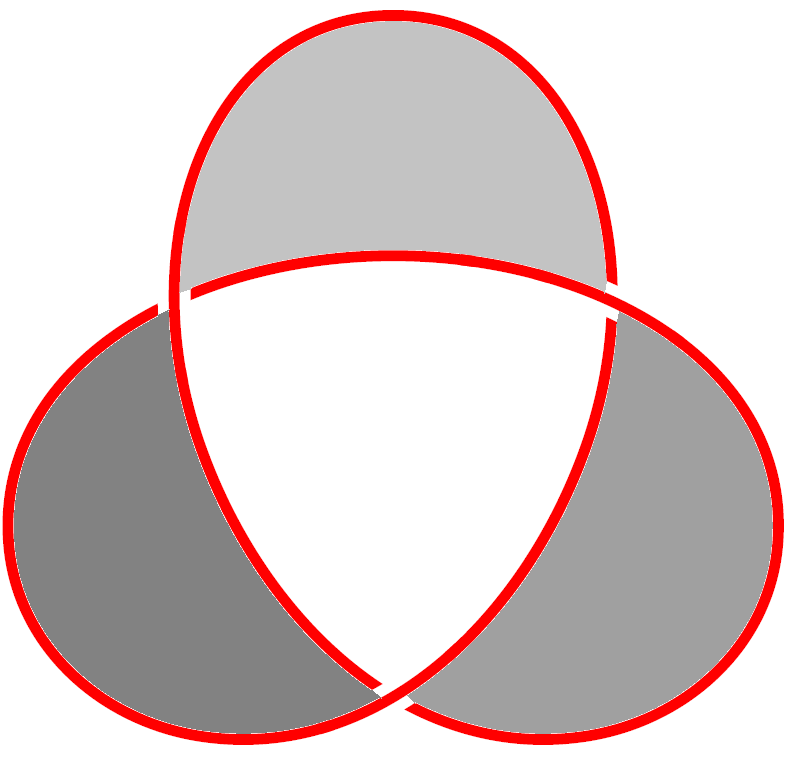
\includegraphics[width= 0.4\linewidth]{seifert1}\quad\quad
		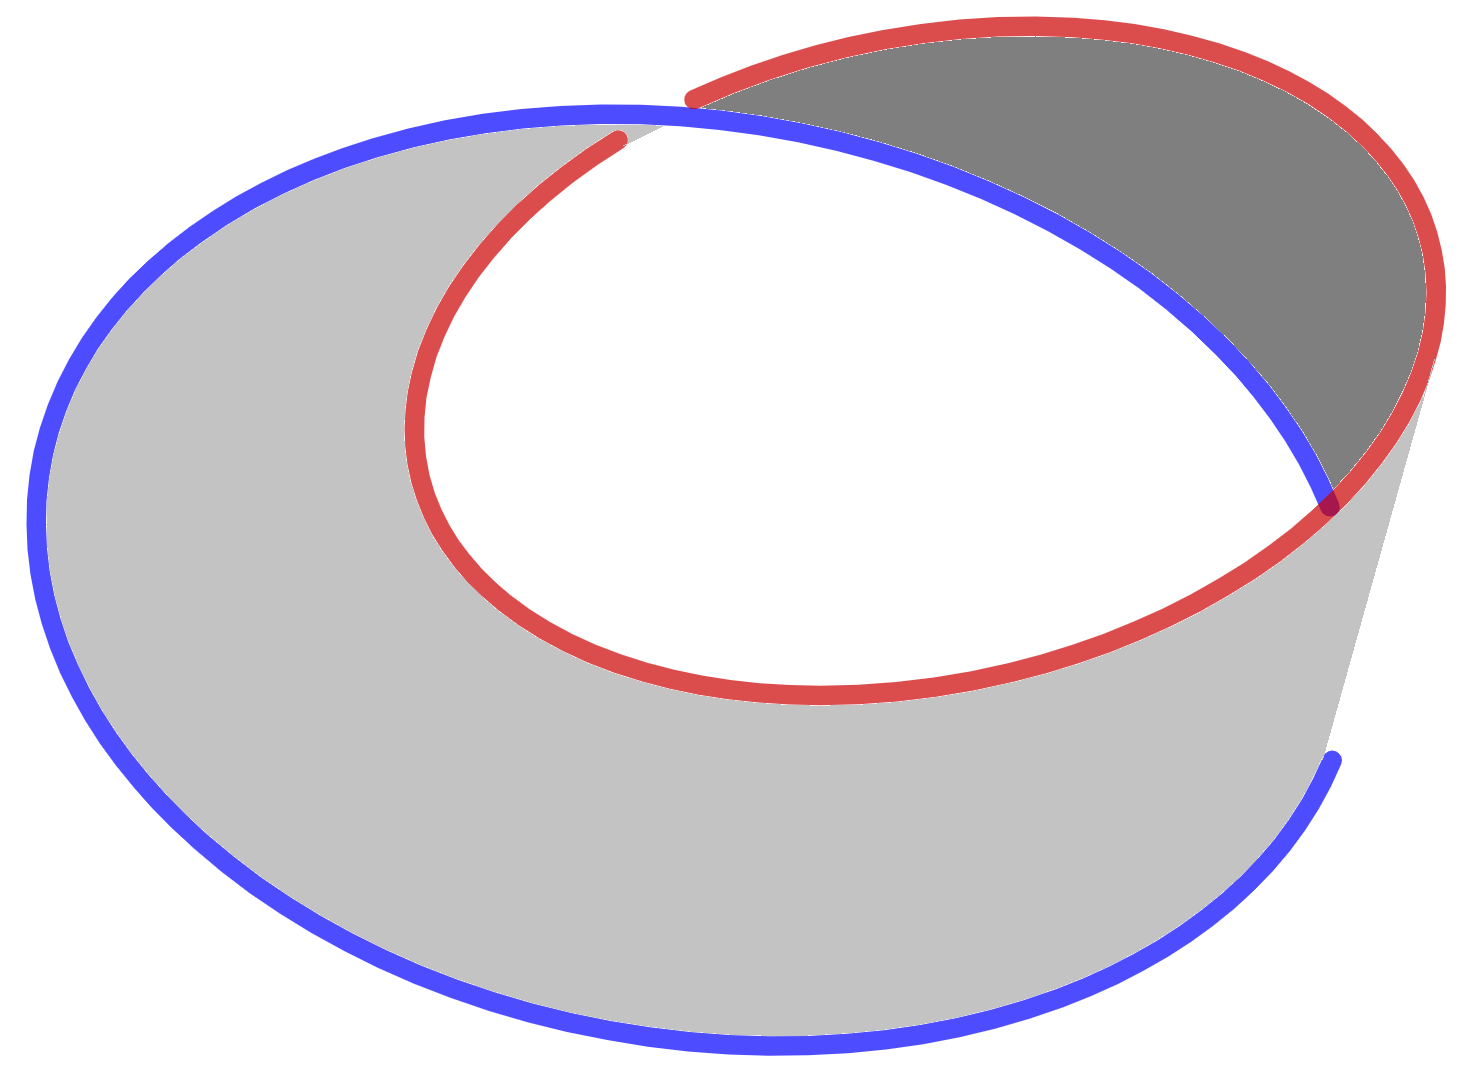
\includegraphics[width= 0.4\linewidth]{seifert2}
		\caption{\small\textit{\color{duongvaotoanhoc}Hình $12$: Mặt Seifert của nút ba lá và của liên kết Hopf (mặt M\"obius).}}
		\vspace*{-10pt}
	\end{figure}
	Sự tương tự tiếp theo: với $p$ là một số nguyên tố, ta xét vành $\mathbb{Z}_p$ các số nguyên $p$--adic cũng như trường $\mathbb{Q}_p$ các số $p$--adic. So với $\text{Spec}(\mathbb{Z})$, phổ $\text{Spec}(\mathbb{Z}_p)$ chỉ còn $2$ điểm là điểm tổng quát $\text{Spec}(\mathbb{Q}_p)$ và điểm đóng $\text{Spec}(\mathbb{F}_p)$, vì thế ta gọi thao tác này {\bf\color{duongvaotoanhoc} địa phương hóa} (tập trung nhìn vào số nguyên tố $p$ và quên đi các số nguyên tố khác). Thao tác này ứng với việc lấy {\bf\color{duongvaotoanhoc} lân cận ống} $V$ của nút, kết quả thu được là một hình xuyến đặc. Dù hình xuyến đặc không đồng phôi với đường tròn, chúng {\bf\color{duongvaotoanhoc} tương đương đồng luân với nhau}, điều này ứng với việc $\text{Spec}(\mathbb{Z}_p)$ và $\text{Spec}(\mathbb{F}_p)$ {\bf\color{duongvaotoanhoc} tương đương đồng luân étale với nhau}. Khi bỏ nút ban đầu khỏi $V$, ta thu được một không gian tương đương đồng luân với mặt xuyến (rỗng). Nhóm cơ bản của mặt xuyến là $\mathbb{Z} \times \mathbb{Z}$, một nhóm được sinh bởi hai phần tử là hai khuyên như trong Hình $13$.
	\begin{figure}[H]
		\vspace*{-5pt}
		\centering
		\captionsetup{labelformat= empty, justification=centering}
		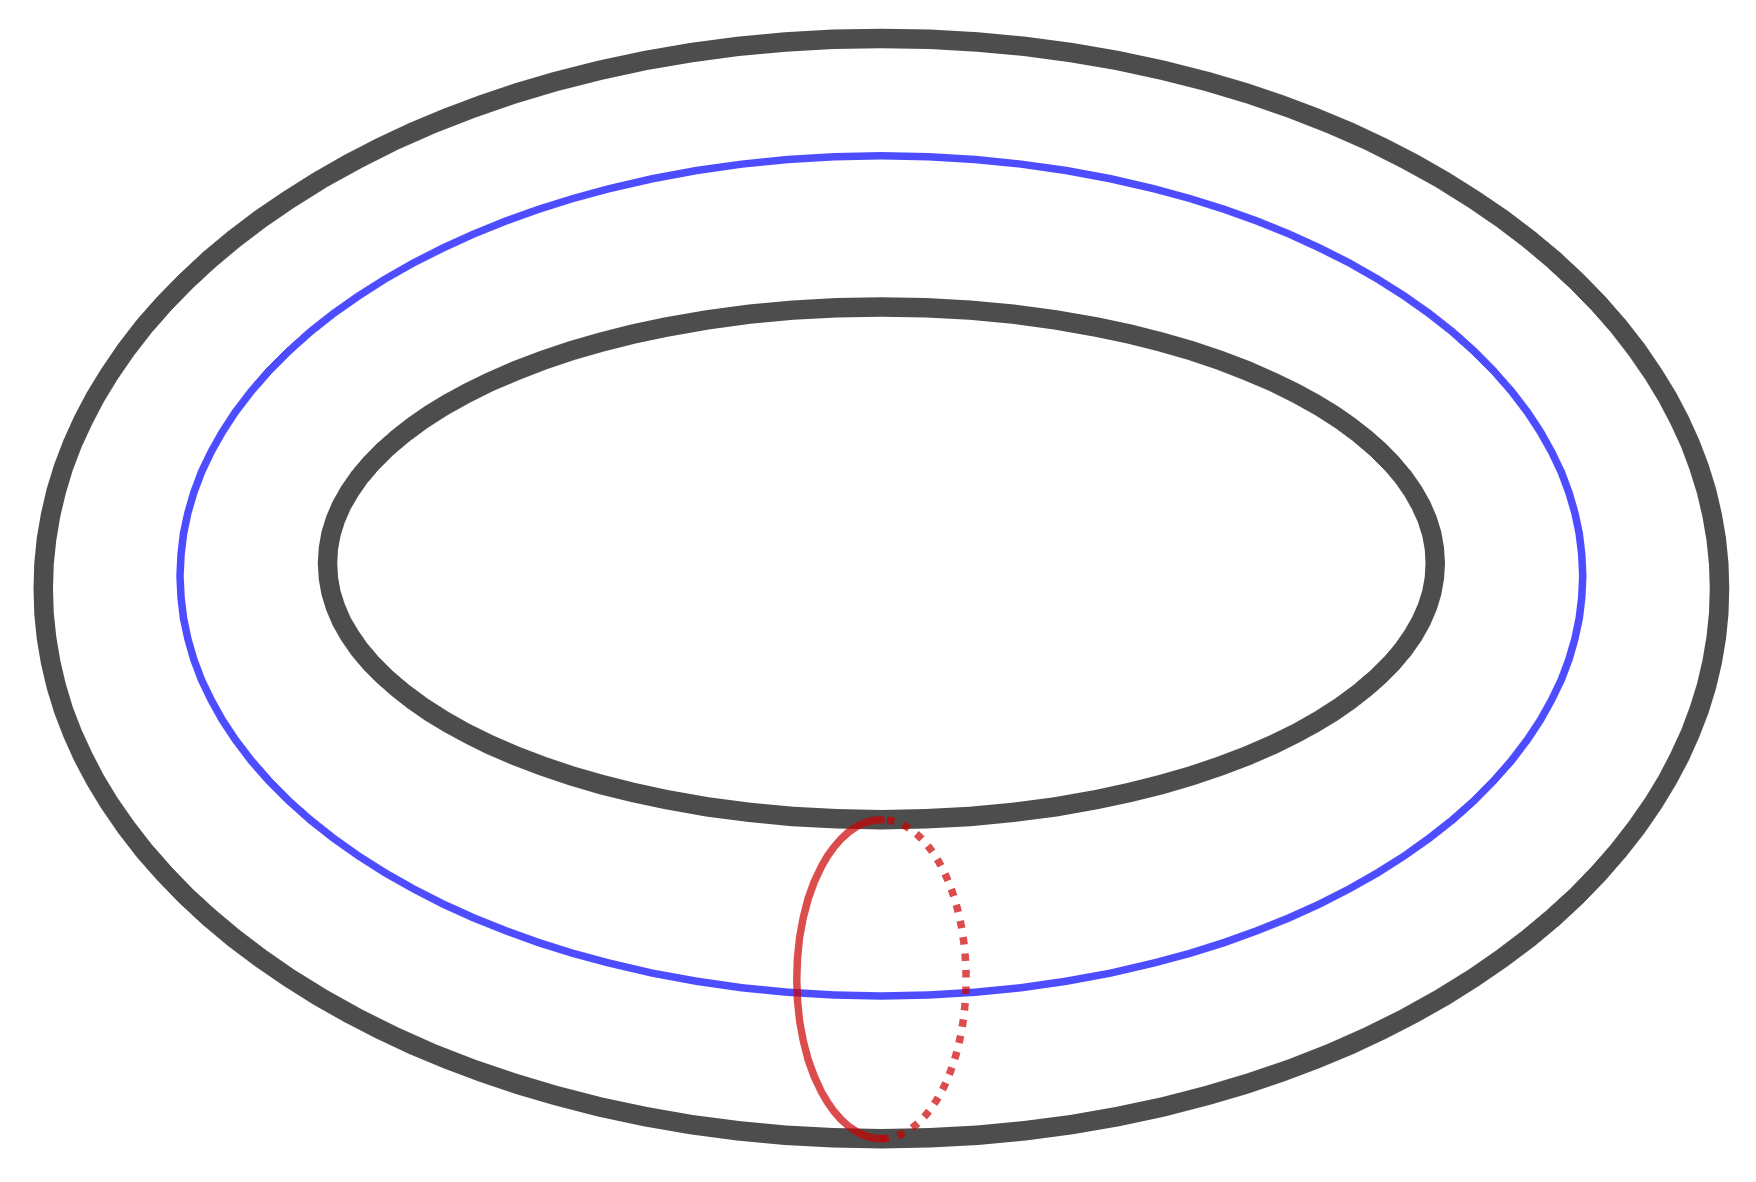
\includegraphics[width= 0.7\linewidth]{h13}
		\caption{\small\textit{\color{duongvaotoanhoc}Hình $13$: Nhóm cơ bản của mặt xuyến được sinh bởi hai khuyên màu xanh và màu đỏ.}}
		\vspace*{-10pt}
	\end{figure}
	Tương ứng, khi bỏ $\text{Spec}(\mathbb{F}_p)$ khỏi $\text{Spec}(\mathbb{Z}_p)$, ta thu được $\text{Spec}(\mathbb{Q}_p)$, và {\bf\color{duongvaotoanhoc} nhóm Galois rẽ nhánh yếu} (một phiên bản nhỏ hơn của nhóm cơ bản étale) của $\mathbb{Q}_p$ cũng được mô tả bởi $2$ phần tử sinh. Sau cùng, lý thuyết trường các lớp địa phương của Tate cho ta các đối ngẫu hoàn hảo giữa đối đồng điều Galois của  $\mathbb{Q}_p$ ở bậc $0$ và bậc $2$, cũng như ở bậc $1$ và chính nó. Tương ứng, ta có đối ngẫu Poincaré cho mặt xuyến, một đa tạp đóng $2$--chiều.
	\vskip 0.1cm
	\textbf{\color{duongvaotoanhoc}Thao tác trên biểu đồ phẳng}
	\vskip 0.1cm
	Quay lại với sự đẳng luân của các nút. Một câu hỏi rất tự nhiên là làm thế nào để chứng minh hai nút không đẳng luân? Đẳng luân vốn là một điều kiện tôpô quá khó sử dụng. Một khó khăn khi sử dụng các biểu đồ phẳng là hai nút đẳng luôn có thể cho hai biểu đồ phẳng trông rất khác nhau. Vậy vấn đề đầu tiên là ta cần tìm cách phân biệt hai nút qua biểu đồ phẳng của chúng (bài toán nhận biết nút). Điều này có thể được thực hiện một cách tổ hợp. Cụ thể, hai biểu đồ phẳng biểu diễn hai nút đẳng luân khi và chỉ khi tồn tại một chuỗi hữu hạn các thao tác thuộc một trong $4$ kiểu, được gọi là các {\bf\color{duongvaotoanhoc} chuyển động Reidemeister}.
	\begin{figure}[H]
		\vspace*{-5pt}
		\centering
		\captionsetup{labelformat= empty, justification=centering}
		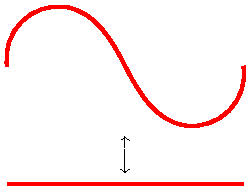
\includegraphics[width= 0.35\linewidth]{R0.pdf}\quad
		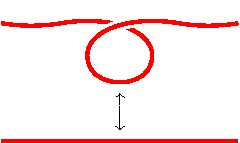
\includegraphics[width= 0.35\linewidth]{R1.pdf}
		\caption{\small\textit{\color{duongvaotoanhoc}R$0$: Phép đẳng luân phẳng.\hspace*{20pt}  RI: Phép xoắn.}}
		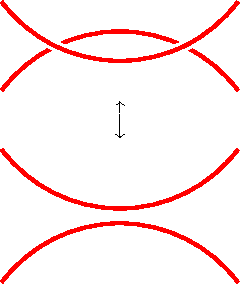
\includegraphics[width= 0.35\linewidth]{R2.pdf}\quad
		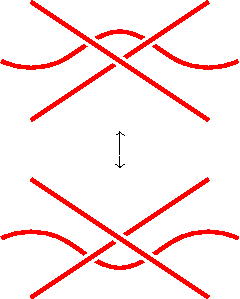
\includegraphics[width= 0.35\linewidth]{R3.pdf}
		\caption{\small\textit{\color{duongvaotoanhoc}RII: Phép đè.\hspace*{30pt} RIII: Phép trượt.}}
		\caption{\small\textit{\color{duongvaotoanhoc}Hình $14$: Các chuyển động Reidemeister.}}
		\vspace*{-10pt}
	\end{figure}
	Từ biểu đồ phẳng của nút, ta dùng các đại lượng không đổi qua các biến đổi Reidemeister, các {\bf\color{duongvaotoanhoc} bất biến nút}. Hai nút có bất biến khác nhau thì phải khác nhau. Một ví dụ như vậy là {\bf\color{duongvaotoanhoc} bất biến tô màu}. Ta nói một biểu đồ phẳng của nút là {\bf\color{duongvaotoanhoc} tô được bằng $3$ màu} nếu mỗi sợi (phần đường cong liên tục giữa hai giao điểm liên tiếp của nút) đều có thể tô được bằng một trong $3$ màu cho trước, sao cho
	\vskip 0.1cm
	$\bullet$ ít nhất hai màu phải được dùng;
	\vskip 0.1cm
	$\bullet$ tại mỗi giao điểm, sợi trên cùng $2$ sợi dưới hoặc là được tô cùng màu, hoặc là được tô $3$ màu khác nhau.
	\vskip 0.1cm
	Ví dụ, nút ba lá hiển nhiên tô được bằng $3$ màu, nút tầm thường hiển nhiên không tô được bằng $3$ màu. Nút số $8$ cũng không tô được bằng $3$ màu. Vậy ít nhất ta biết rằng nút $3$ lá không đẳng luân với nút tầm thường cũng như nút số $8$.
	\vskip 0.1cm
	Hiển nhiên là bất biến tô màu chỉ cho phép phân loại các nút thành $2$ lớp. Ta cần các loại bất biến khác. Ví dụ, xét nút ba lá trái và ảnh gương của nó là nút ba lá phải. Tất nhiên cả hai đều tô được bằng $3$ màu. Rất ngạc nhiên, hai nút này không đẳng luân! Hãy thử dùng các biến đổi Reidemeister để gỡ nút này thành nút kia và bạn sẽ sớm bị thuyết phục. Một bất biến cho phép phân biệt hai nút này là {\bf\color{duongvaotoanhoc} đa thức Alexander}. Đa thức này đến từ {\it lý thuyết Alexander--Fox}, và người ta phát hiện ra phiên bản số học của nó là {\it lý thuyết Iwasawa}. Sự song song của chúng cho phép ta dịch các kết quả từ một bên sang bên còn lại.
	\begin{figure}[H]
		\vspace*{-5pt}
		\centering
		\captionsetup{labelformat= empty, justification=centering}
		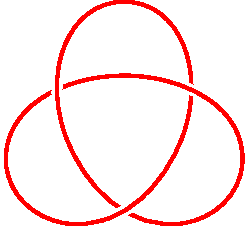
\includegraphics[width= 0.38\linewidth]{trefoil.pdf}\quad\quad
		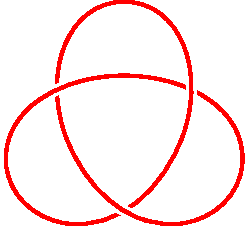
\includegraphics[width= 0.38\linewidth]{mirror trefoil.pdf}
		\caption{\small\textit{\color{duongvaotoanhoc}Hình $15$: Nút ba lá trái và nút ba lá phải.}}
		\vspace*{-10pt}
	\end{figure}
	Một kiểu bất biến khác cho liên kết là {\bf\color{duongvaotoanhoc} số liên kết}. Xét một liên kết được tạo bởi hai nút. Giữa hai nút $L$ và $K$, ta có thể định nghĩa {\bf\color{duongvaotoanhoc} số liên kết} qua biểu đồ phẳng của chúng như sau. Chẳng hạn, tô màu đỏ cho $L$ và màu xanh cho $K$, đồng thời định hướng cho chúng (mỗi nút có thể có $1$ trong $2$ hướng). Tại các điểm trên biểu đồ phẳng mà có một sợi của nút này nằm trên một sợi của nút kia hoặc ngược lại, ta đánh dấu $+$ hoặc $-$ theo quy tắc ở Hình $16$. Sau đó ta lấy số dấu cộng trừ đi số dấu trừ, và lấy kết quả chia đôi. Kết quả cuối cùng thu được được gọi là số liên kết $\text{lk}(L,K)$. Chẳng hạn, số liên kết của hai nút trong liên kết Hopf là $1$ hoặc $-1$, tùy theo cách định hướng hai nút.
	\begin{figure}[H]
		\vspace*{-5pt}
		\centering
		\captionsetup{labelformat= empty, justification=centering}
		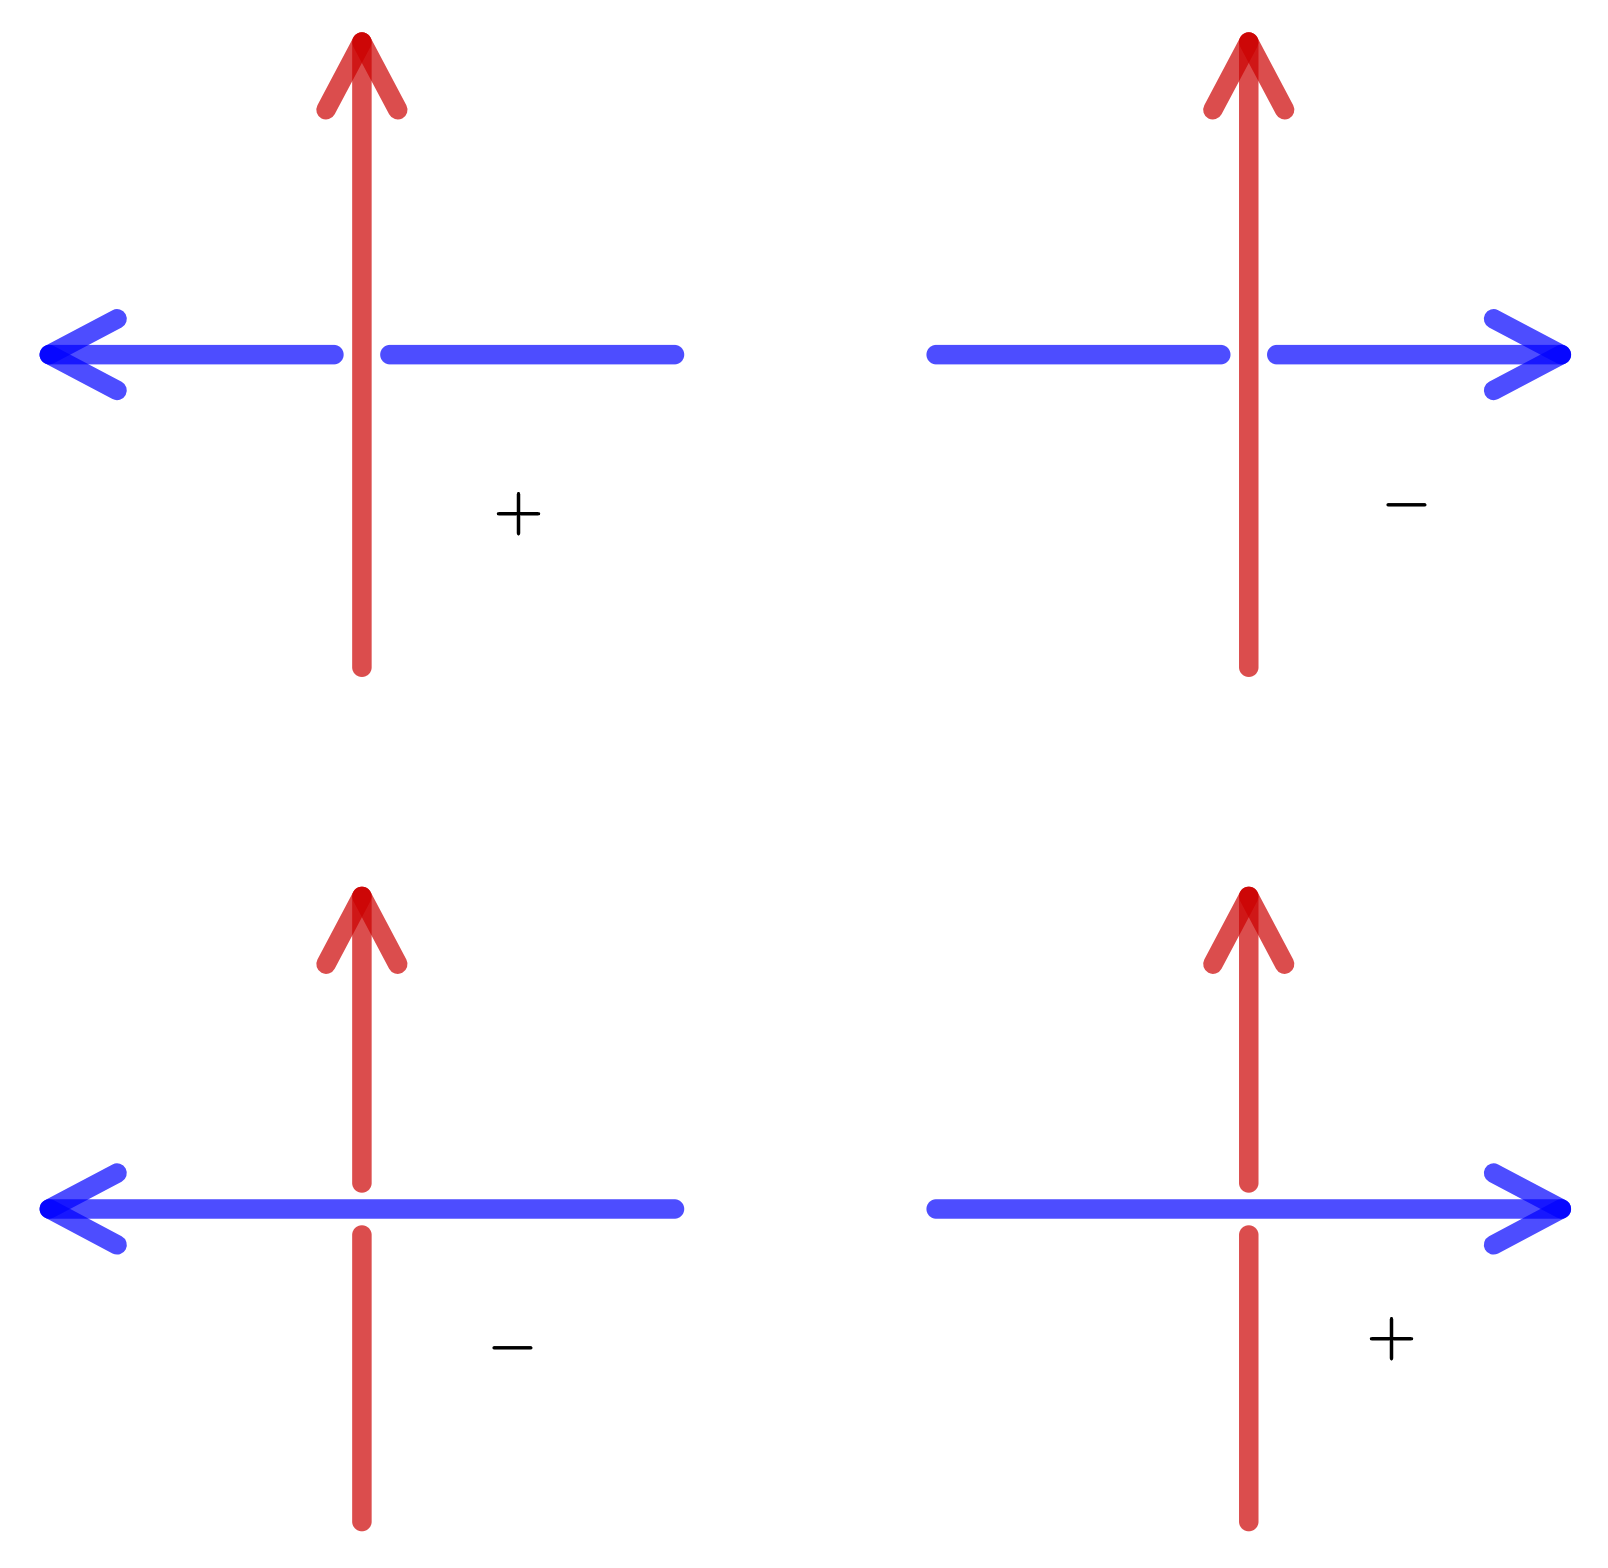
\includegraphics[width= 0.65\linewidth]{h16}
		\caption{\small\textit{\color{duongvaotoanhoc}Hình $16$: Quy tắc tính số liên kết.}}
		\vspace*{-10pt}
	\end{figure}
	Nhiều tính toán cho thấy rằng số liên kết thỏa mãn các tính chất tương tự như {\bf\color{duongvaotoanhoc} ký hiệu Legendre} $\left(\dfrac{p}{q}\right)$ giữa hai số nguyên tố $p, q$ trong lý thuyết thặng dư bậc hai. Ta có thể chứng minh rằng $\text{lk}(K,L) = \text{lk}(L,K)$. Tương ứng, ta có luật tương hỗ bậc hai, nói rằng 
	\begin{align*}
		\left(\dfrac{p}{q}\right) = (-1)^{\tfrac{(p-1)(q-1)}{4}}\left(\dfrac{q}{p}\right).
	\end{align*}
	Bài toán trung tâm của tôpô số học có lẽ là câu hỏi tự nhiên nhất: số nguyên tố nào ứng với nút nào? Đây vẫn là một câu hỏi mở. Nếu một ngày người ta xây dựng được một tương ứng $1-1$ tốt giữa chúng, theo nghĩa mỗi kết quả với số nguyên tố thì ta có kết quả với các nút tương ứng, một số lượng khổng lồ bài toán tôpô học sẽ được giải bằng các kết quả tương tự ở lý thuyết số, và ngược lại. Có thể nói, tôpô số học là một trong những ví dụ điển hình nhất về tư tưởng toán học thống nhất, rằng tất cả những đại số, giải tích, hình học, số học... đều chỉ là một.
\end{multicols} 
%	\newpage

	\setcounter{figure}{0}
	\thispagestyle{quantoannone}
\pagestyle{quantoan}
\everymath{\color{quantoan}}
\graphicspath{{../quantoan/pic/}}
%\blfootnote{\color{quantoan}\color{quantoan}$^*$Nguồn Math. Intellegencer, Số $41$.}
\begingroup
\AddToShipoutPicture*{\put(0,616){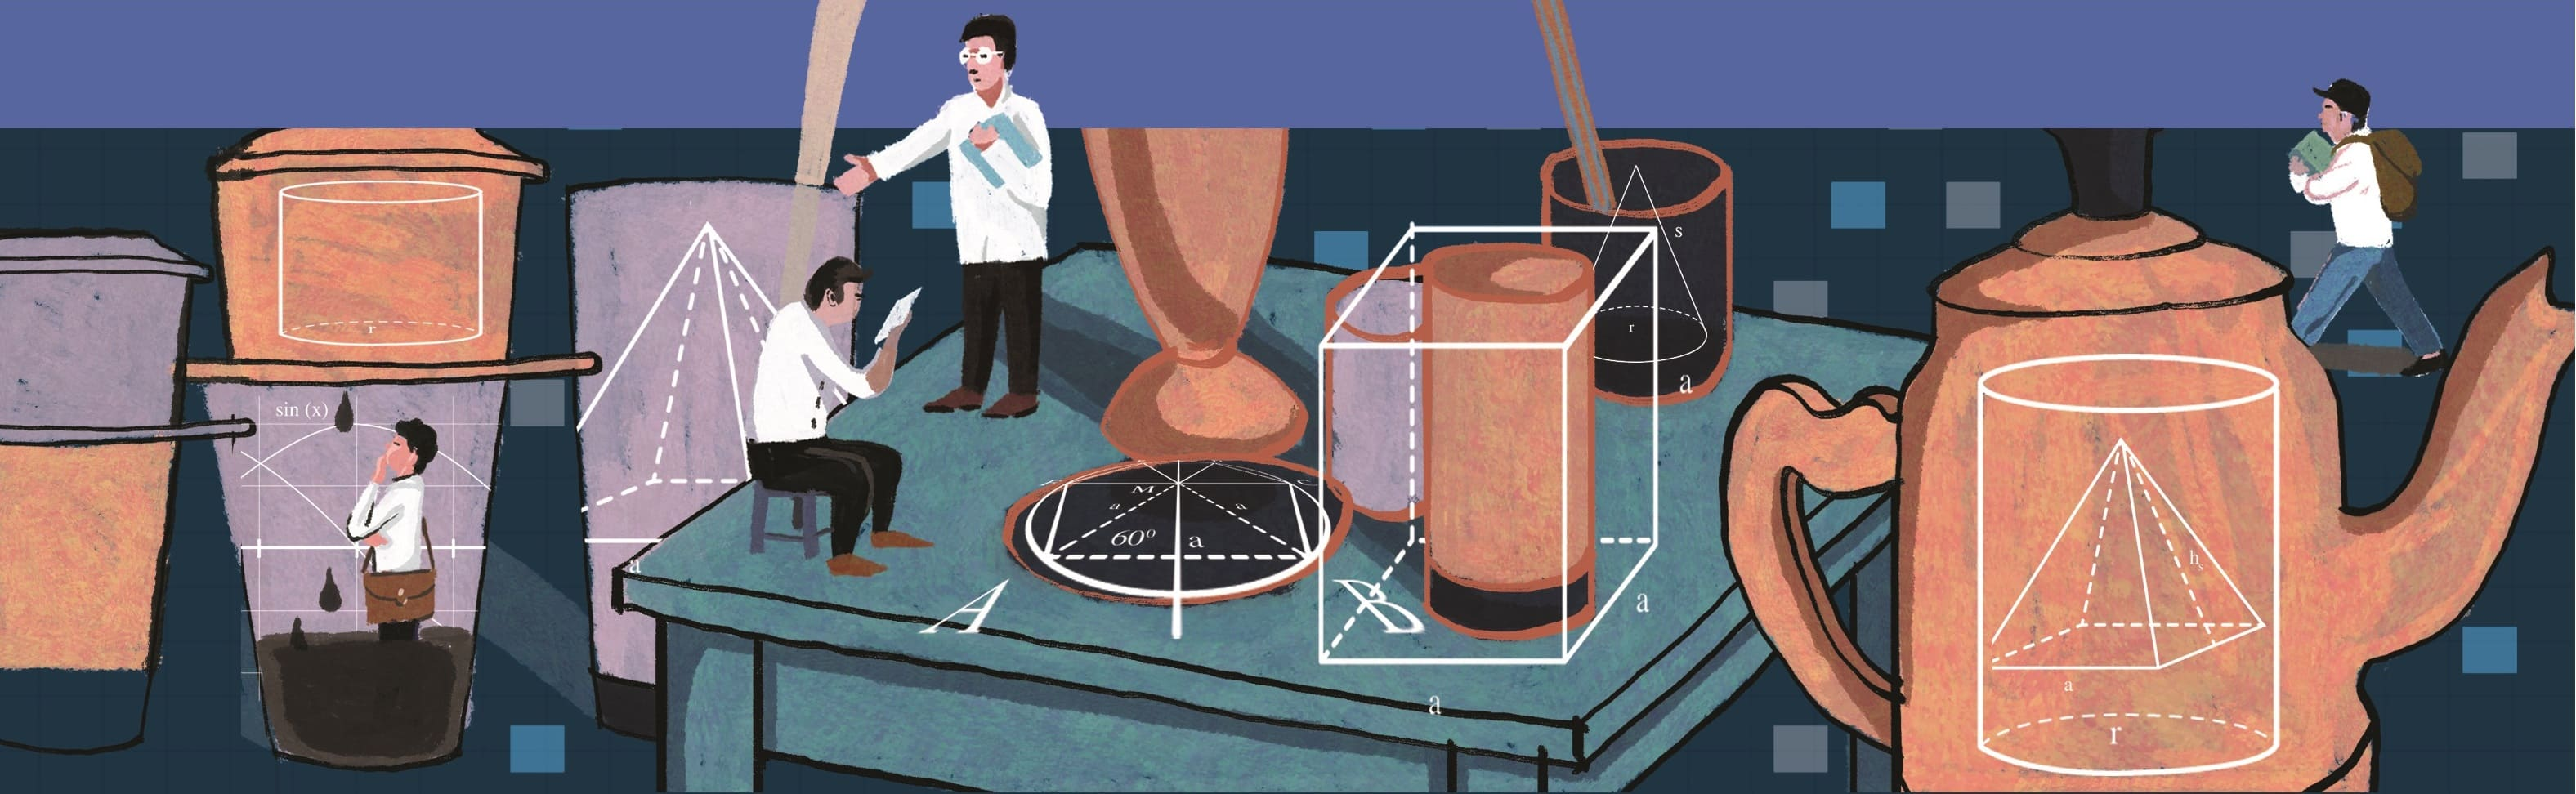
\includegraphics[width=19.3cm]{../bannerquantoan}}}
\AddToShipoutPicture*{\put(104,495){
\includegraphics[scale=1]{../tieude.pdf}}}
\centering
\endgroup

\vspace*{218pt}
\textit{\textbf{\color{quantoan}LTS.} Chuyên mục Danh ngôn Toán học giới thiệu với bạn đọc về lịch sử, ý nghĩa của những phát ngôn bởi các nhà toán học nổi tiếng. Ban biên tập Pi trân trọng mời bạn đọc đóng góp cho chuyên mục này.}

\vspace*{-5pt}
\begin{multicols}{2}
	Vào khoảng ba thế kỷ trước Công nguyên có một người Hy Lạp tên là Euclid từ xứ Alexandria. Họ gọi ông là như vậy, vì không ai biết họ của ông là gì. Ông lang thang ở thành Alexandria và trong thời gian rỗi, ông đã viết ra một bộ sách giáo khoa về hình học mà ông đặt tên là Cơ sở. Có lẽ ông đã được đào tạo sớm từ các học trò của Plato ở Athens, sau đó tiếp tục thành lập một trường học ở Alexandria vào năm $306$ trước Công nguyên. 
	\vskip 0.1cm
	Vào thời đó, có một nhà cai trị và tướng quân người Macedonia thuộc Hy lạp  là Ptolemy I Soter . Ông từng là vệ sỹ riêng của Alexander Đại đế, cũng đồng thời là một pharaoh của Ai Cập. Ptolemy I, giống như Alexander, rất quan tâm đến việc thúc đẩy nghiên cứu học thuật, và ông là người bảo trợ cho việc khai phá tri thức, sáng lập ra Đại Thư viện Alexandria. Ông ta tập hợp những ``người có học" xung quanh cung đình của mình.  Những người được biết đến là ``các bạn bè" này, bất kể là người đó là quý tộc hay thường dân, phục vụ Ptolemy với vai trò là các cố vấn chính của ông. Danh tiếng về bản tính nhân từ và phóng khoáng của tướng quân Ptolemy I đã gắn kết tầng lớp lính tráng trôi nổi nay đây mai đó, gồm cả những người Macedonia và những người Hy Lạp khác  tới phục vụ quanh ông. Chính Ptolemy đã viết cuốn Sử lược về các chiến dịch của Alexander, đã thất truyền. Đây từng được coi là một tác phẩm khách quan, nổi bật bởi tính trung thực và sự tỉnh táo trong nhận định. 
	\begin{figure}[H]
		\vspace*{-5pt}
		\centering
		\captionsetup{labelformat= empty, justification=centering}
		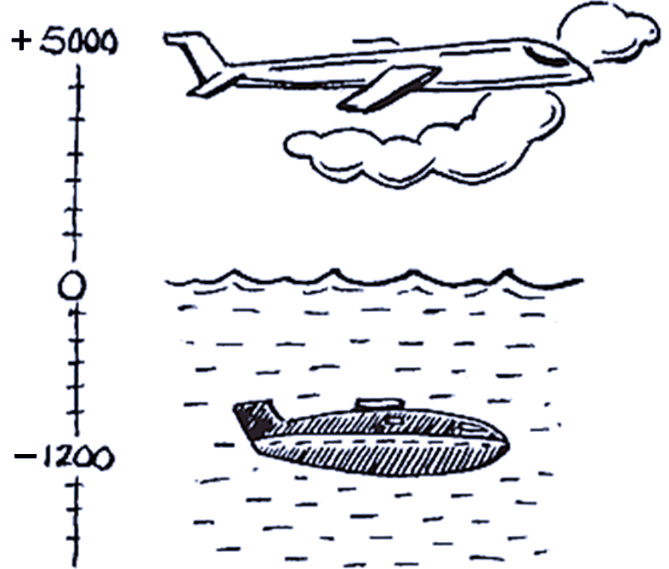
\includegraphics[width= 1\linewidth]{1}
		\caption{\small\textit{\color{quantoan}Hình $1$. Ptolemy I Soter ($366-282$ TCN), vị pharaoh Ai cập đồng thời là tướng quân người Macedonia thuộc Hy lạp.}}
		\vspace*{-12pt}
	\end{figure}
	Ptolemy I cũng  từng mời Triết gia nổi tiếng Strabo đến Alexandria làm gia sư cho con trai mình. Và khá đặc biệt, nhà toán học Euclid cũng là một trong những học giả được Prolemy bảo trợ. Tướng quân Ptolemy thấy tác phẩm tiêu biểu của Euclid, cuốn Cơ sở, quá khó để lĩnh hội, vì vậy ông ta  đã hỏi liệu có cách nào dễ dàng hơn để nắm vững được nó không. Và Euclide, theo ghi chép lại của Triết gia Proclus, đã có câu nói châm biếm nổi tiếng sau để trả lời Ptolemy ``Thưa Đức Ngài, không có con đường hoàng gia nào dẫn tới hình học".
	\begin{figure}[H]
		\vspace*{-5pt}
		\centering
		\captionsetup{labelformat= empty, justification=centering}
		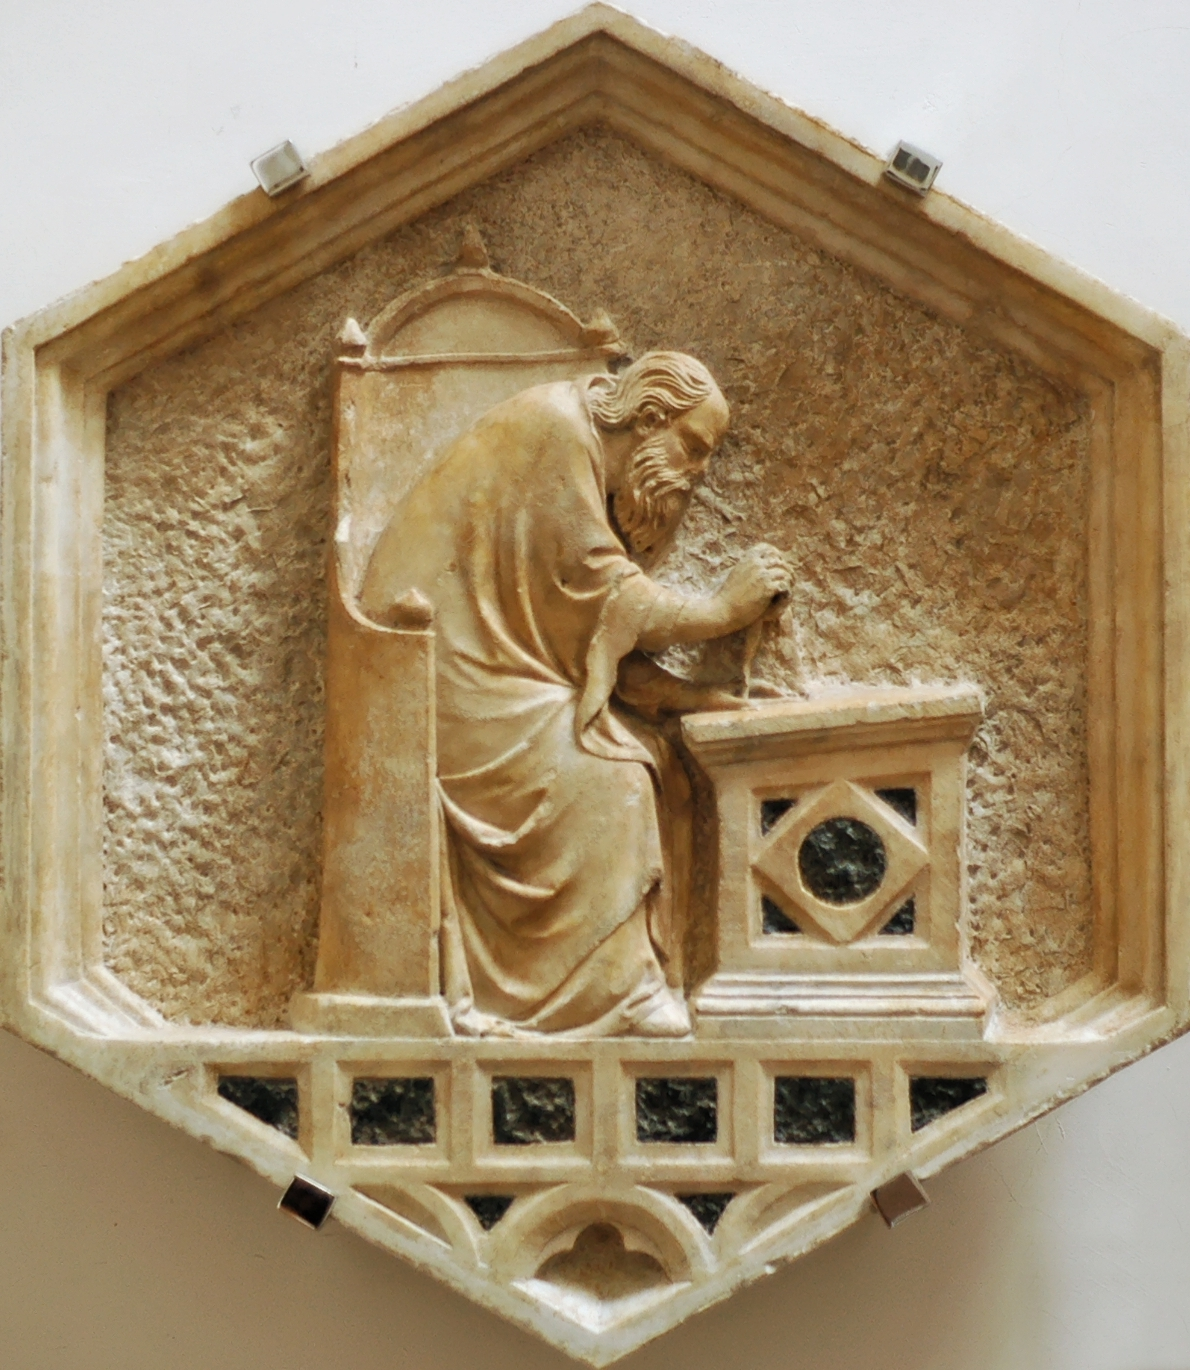
\includegraphics[width= 0.6\linewidth]{4}
		\caption{\small\textit{\color{quantoan}Hình $3$. Euclid, hay Kiến trúc. Tranh đá cẩm thạch, tầng hầm tháp chuông Florence, Ý.}}
		\vspace*{-10pt}
	\end{figure}
	Cụm từ ``con đường hoàng gia" thời đó chỉ  con đường đặc biệt được xây dựng xuyên qua Anatolia và Ba Tư bởi Darius Đại đế của Ba Tư (Darius I), cho phép liên lạc và chuyển quân nhanh chóng, nhưng Euclide đã sử dụng từ Hy lạp  ἀτραπός nghĩa là ``lối đi" (chứ không phải từ ὁδός ``con đường")  để truyền đạt ý nghĩa của ``đường tắt".
	\begin{figure}[H]
		\vspace*{-5pt}
		\centering
		\captionsetup{labelformat= empty, justification=centering}
		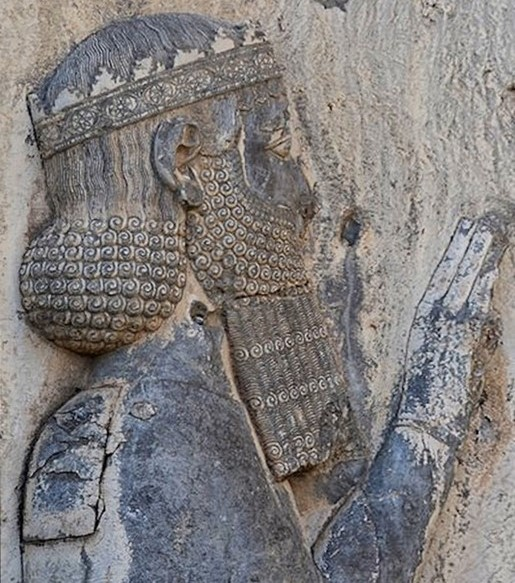
\includegraphics[width= 0.6\linewidth]{2}
		\caption{\small\textit{\color{quantoan}Hình $3$. Darius Đại đế của Ba Tư ($550-486$ TCN).}}
		\vspace*{-10pt}
	\end{figure}
	Tất nhiên, Eclide đã  nói bằng tiếng Hy Lạp với hy vọng Ptolemy sẽ hiểu ra rằng không có một điểm thưởng nào cho những ai chỉ đơn giản có mặt để điểm danh qua loa, khi muốn học môn hình học cho đến nơi đến chốn.
	\vskip 0.1cm
	Rất thú vị, ngày nay cụm từ ``con đường hoàng gia" đã vượt qua khuôn khổ của hình học và toán học, với ý nghĩa mới là ``con đường dẫn tới đích dễ dàng và nhanh nhất, không tốn công sức". Người ta có thể nói, ``đội bóng, sau khi đã loại tất cả các đối phương trong cùng nhóm, hiện đang trên con đường hoàng gia dẫn tới chức vô địch lần đầu tiên trong lịch sử thông qua đá loại trực tiếp", ``hãng phim nọ đang trên con đường hoàng gia đơn độc thống trị cả nền sản xuất điện ảnh và  tạo ra một thế độc quyền trong nền công nghiệp mà họ đang tích cực khai thác". Và tất nhiên, khi học tiếng Anh, các bạn cũng đều biết tới câu nói ``there is no royal road to learning". Học tiếng Anh, cũng như học hình học, đòi hỏi phải luyện tập kiên trì để đạt tới thành công trong việc diễn tả lưu loát những ý nghĩ riêng của bản thân mà không phải học thuộc lòng những cách nói mẫu, tuy đẹp nhưng khác lạ với cách diễn đạt của chính mình. 
	\begin{figure}[H]
		\vspace*{-5pt}
		\centering
		\captionsetup{labelformat= empty, justification=centering}
		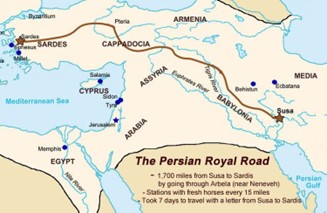
\includegraphics[width= 1\linewidth]{3}
		\caption{\small\textit{\color{quantoan}Hình $4$. Con đường hoàng gia của Ba Tư.}}
		\vspace*{-10pt}
	\end{figure}
	Còn trong môn hình học, cần rất nhiều kiên trì để hiểu và ghi nhớ những điều phức tạp của môn học, bao gồm các tính chất khác nhau của các hình khác nhau có hai chiều và ba chiều. Chỉ khi đó chúng ta mới có thể học được cách dựng và phân tích các hình hình học.
\end{multicols}
	\newpage
	
%	\setcounter{figure}{0}
%	\thispagestyle{toancuabinone}
\pagestyle{toancuabi}
\everymath{\color{toancuabi}}
%\blfootnote{$^1$\color{toancuabi}Đại học Thăng Long.}
\graphicspath{{../toancuabi/pic/}}
\begingroup
\AddToShipoutPicture*{\put(0,616){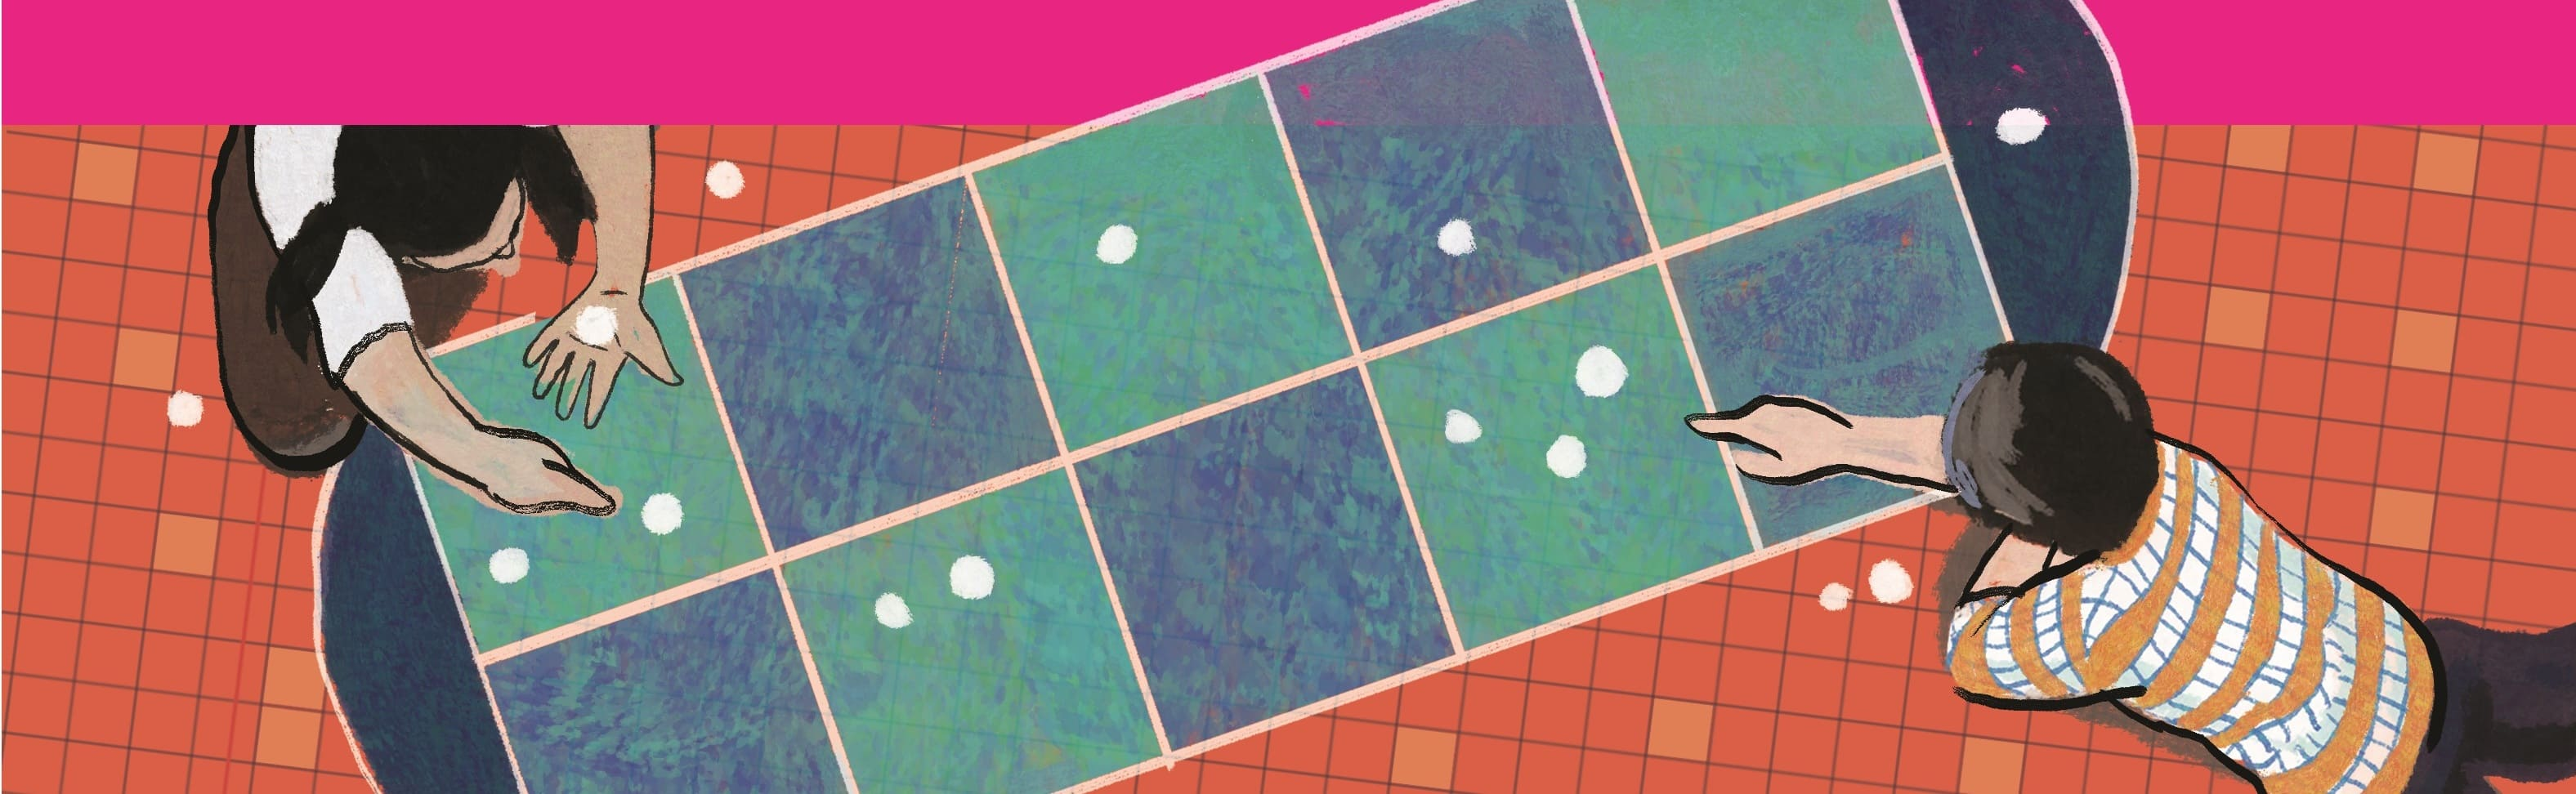
\includegraphics[width=19.3cm]{../bannertoancuabi}}}  
\AddToShipoutPicture*{\put(130,555){
\includegraphics[scale=1]{../tieude.pdf}}} 
\centering
\endgroup
\vspace*{150pt}

\begin{multicols}{2}
	Lần này thì Thám tử Xuân Phong phải vào tận hang ổ của một băng đảng để điều tra manh mối về một vụ án. Khác với những lần bị lạc lên đảo, ở đó có những thổ dân nói thật hoặc nói dối, trong ba người thuộc  băng đảng mà Xuân Phong tiếp cận, không có ai nói thật mà lại có tới ba kiểu người. Loại thứ nhất, tất nhiên rồi, đó là người Nói dối -- chuyên nói sai sự thật. Tiếp theo mới phức tạp cho Xuân Phong, lại có kẻ Ranh mãnh: hắn sẽ nói thật hoặc nói dối bất cứ khi nào hắn muốn. Thế chưa hết, loại cuối cùng mới rầy rà, đó là người Thay đổi, cứ nói thật và nói dối luân phiên nhau. Nhiệm vụ của Thám tử là xác định  từng người thuộc kiểu gì. Vừa được miêu tả về ba kiểu người như vậy, thanh tra Lê Kính đã ôm đầu kêu rên: ``Thôi, thà cho tôi lên hoang đảo với thổ dân nói Thật và nói Dối rõ ràng còn hơn. Ở đây phức tạp tờ mờ quá, không biết đường nào mà lần!"
	\vskip 0.1cm
	Xuân Phong đưa tay trấn an sự bực tức nóng nảy của thanh tra Lê Kính, thì thầm nói: ``Anh cứ yên tâm. Thế giới của băng đảng này phức tạp như vậy, nhưng tôi quả quyết chỉ sau không quá ba câu hỏi, ta sẽ biết ngay ai là thuộc loại người nào?"
	\vskip 0.1cm
	Làm thế nào mà Xuân Phong lại tự tin như thế nhỉ? Em có thể tìm thấy cách Thám tử đặt câu hỏi để xác định ai là ai, và giúp Lê Kính lấy lại bình tĩnh hay không?
\end{multicols}
\begin{figure}[H]
	\centering
	\vspace*{-5pt}
	\captionsetup{labelformat= empty, justification=centering}
	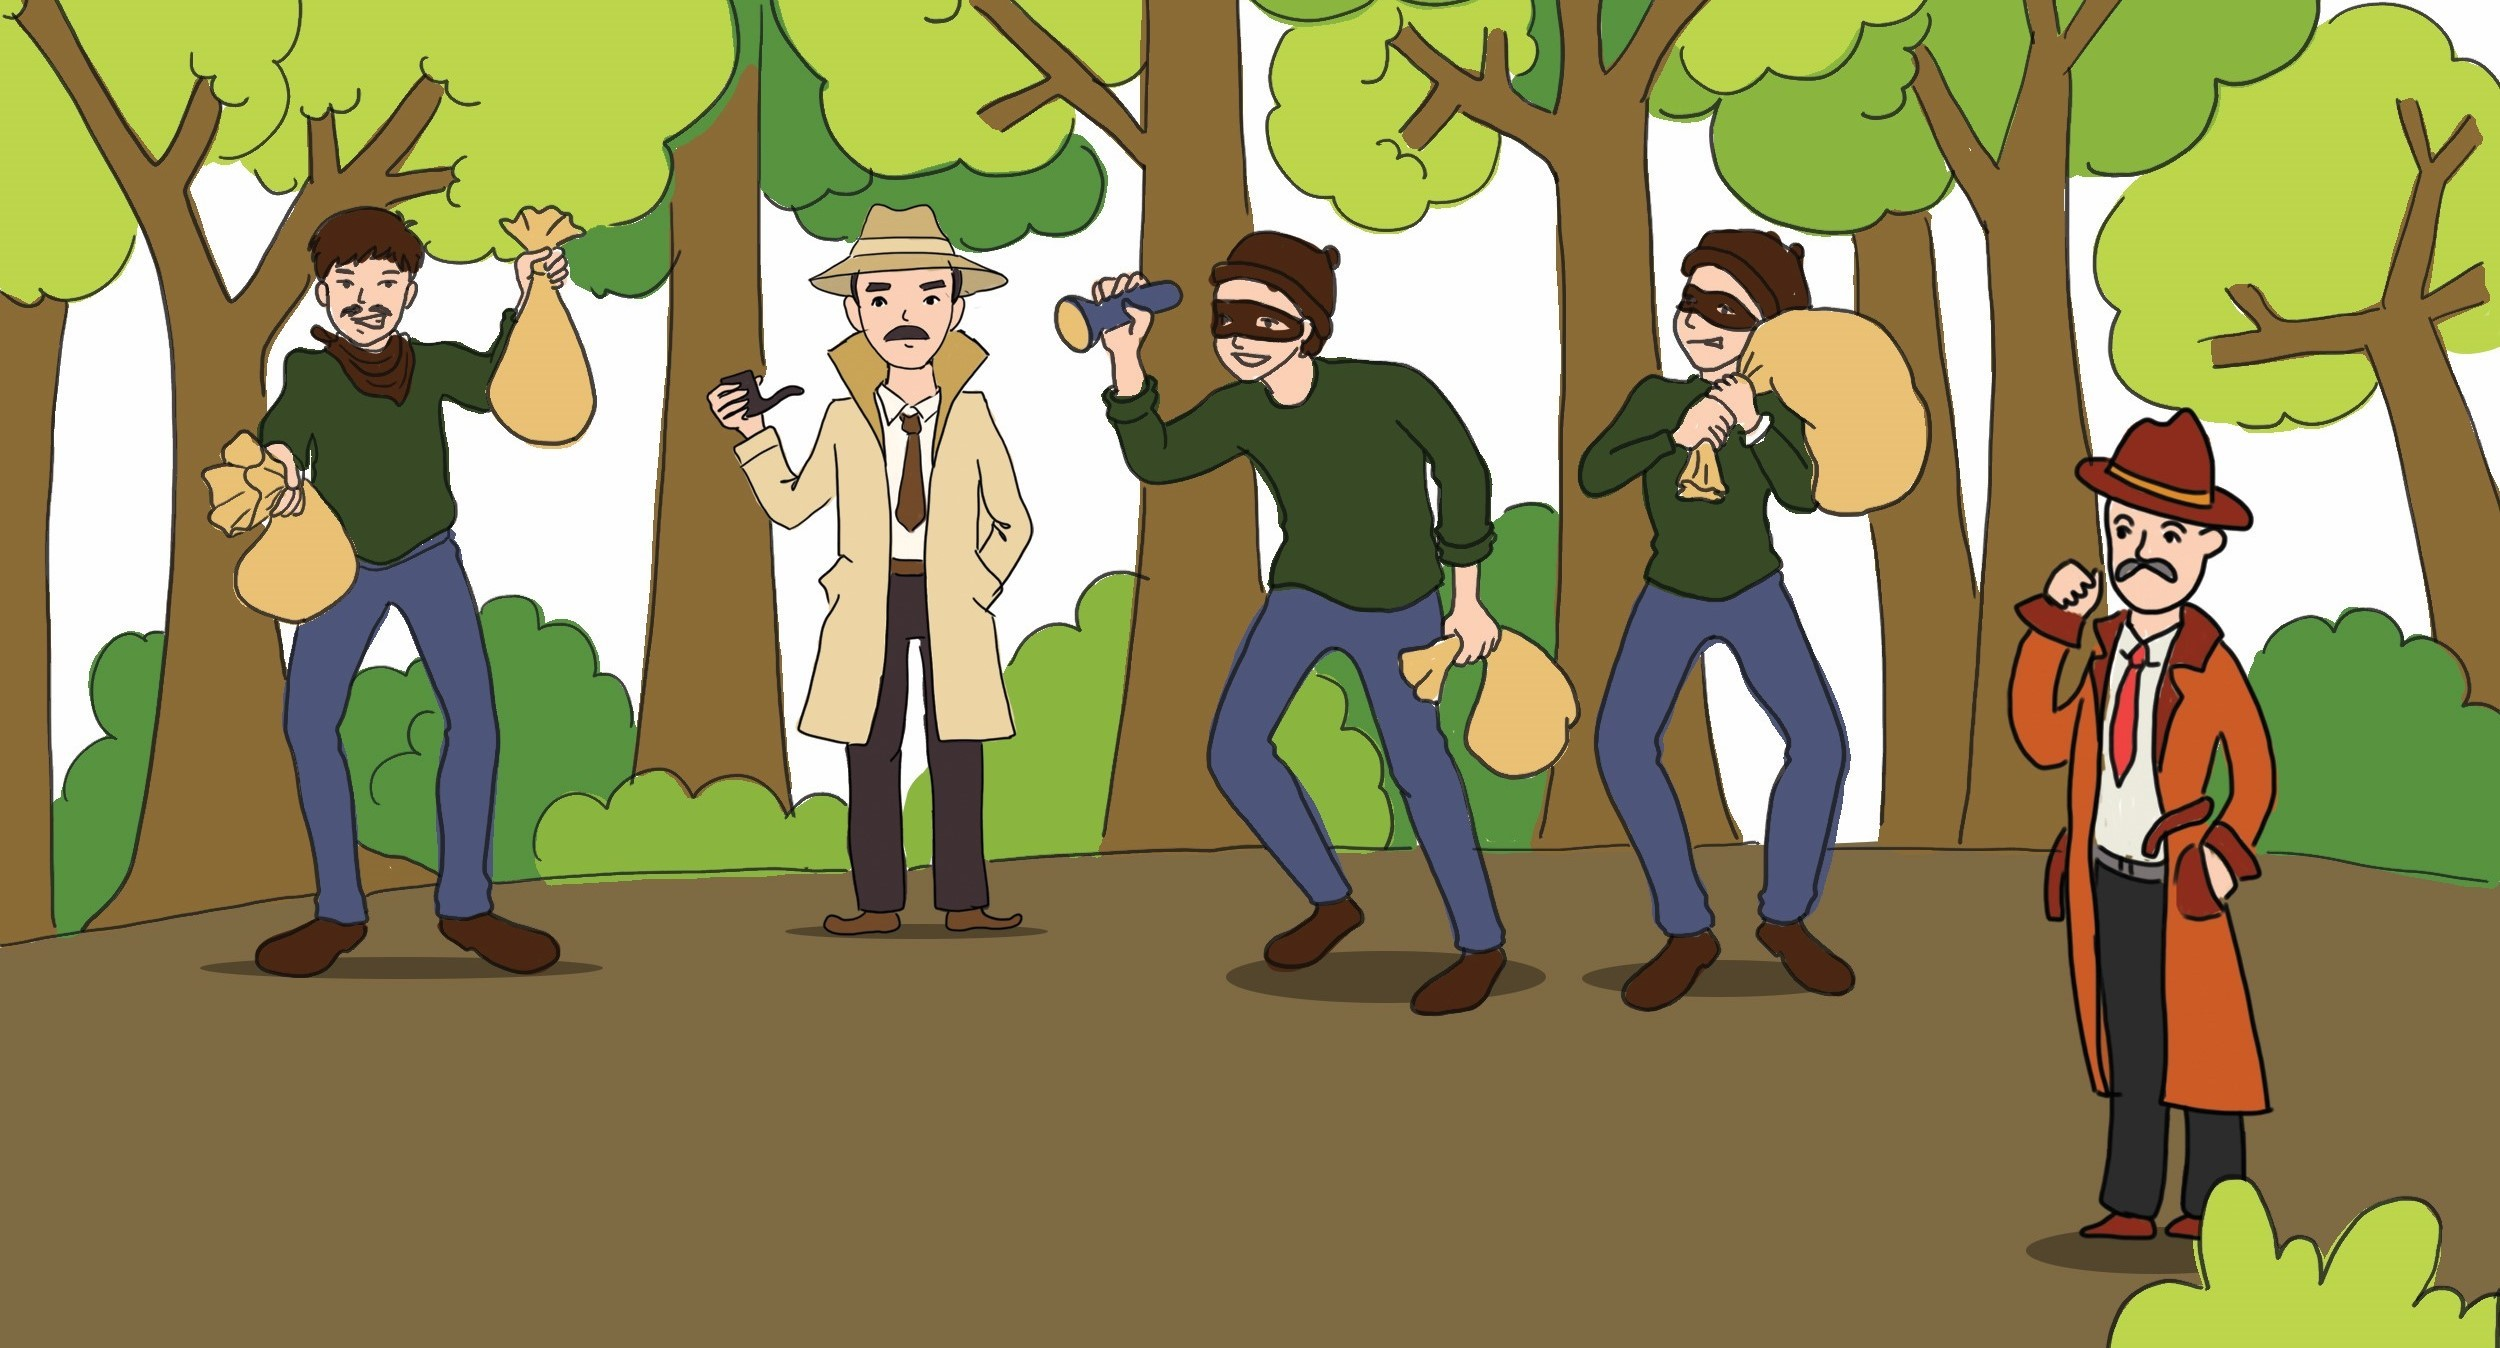
\includegraphics[width=0.98\linewidth]{xuanphong}
	\vspace*{-10pt}
\end{figure}
\newpage
\begingroup
\AddToShipoutPicture*{\put(115,670){\includegraphics[scale=1]{../tieude11.pdf}}} 
\centering
\endgroup
\vspace*{33pt}

\begin{multicols}{2}
	$\pmb{1.}$	Pinocchio và Pierrot thi chạy với nhau. Pierrot chạy suốt cả quãng đường với cùng một tốc độ, còn Pinocchio chạy nhanh gấp đôi Pierrot trong nửa đầu quãng đường, và nửa sau lại chậm bằng nửa Pierrot. Hỏi ai đã thắng?
	\begin{figure}[H]
		\centering
		\vspace*{-5pt}
		\captionsetup{labelformat= empty, justification=centering}
		\includegraphics[width=1\linewidth]{Pi4_bai1}
		\vspace*{-15pt}
	\end{figure}
	$\pmb{2.}$ ``Còn quá sớm để các em nhìn thấy điều thần kỳ sau đây của thế giới pháp sư," cô giáo McGonagall  nói với $33$ học trò của mình ở ngôi trường Hogwarts đào tạo Phù thủy, và vung cây đũa thần ra lệnh: ``Nào, các em hãy nhắm mắt lại!" Tất cả học trò nam và một phần ba học trò nữ đều nhắm mắt phải. Tất cả học trò nữ và một phần ba các học trò nam đều nhắm mắt trái. Hỏi có bao nhiêu học trò đã nhìn thấy những gì còn quá sớm để nhìn thấy?
	\begin{figure}[H]
		\centering
		\vspace*{-10pt}
		\captionsetup{labelformat= empty, justification=centering}
		\includegraphics[width=1\linewidth]{Pi4_bai2}
		\vspace*{-15pt}
	\end{figure}
	$\pmb{3.}$ 	Bác Tư múc ra ba thìa sữa từ một ly sữa đầy và đổ chúng một ly đựng cà phê nguyên chất và khuấy đều. Sau đó bác múc ba thìa hỗn hợp thu được và đổ lại vào ly sữa. Hỏi bây giờ thứ gì nhiều hơn: cà phê trong ly đựng sữa hay sữa trong ly đựng cà phê?
	\begin{figure}[H]
		\centering
		\vspace*{5pt}
		\captionsetup{labelformat= empty, justification=centering}
		\includegraphics[width=1\linewidth]{Pi4_bai3}
		\vspace*{-15pt}
	\end{figure}
	$\pmb{4.}$ Ma xó Brownie là một nhân vật trong văn hóa dân gian Anh và một số quốc gia khác. Đó là một dạng Phúc thần (ma thiện), tiểu yêu nghịch ngợm, thường mô tả là bé tí hon, có da nâu, ăn mặc tuềnh toàng, sinh sống gần gũi với con người, và là thần hộ mệnh cho các gia đình. Các Brownies có một xã hội thu nhỏ riêng và thường tổ chức những cuộc họp bí mật tại một tảng đá nào đó để con người không để ý tới. 
	\vskip 0.1cm
	Trong một tòa nhà bảy tầng nọ cũng có rất nhiều ma xó Brownies sinh sống. Thang máy chạy giữa tầng một và tầng cuối, dừng lại ở mỗi tầng. Ở mỗi tầng, bắt đầu từ tầng đầu tiên, có một chú Brownie bước vào thang máy, nhưng không có chú nào bước ra ngoài. Thang máy cứ di chuyển liên tục như vậy cho đến khi chú Brownie thứ một nghìn bước vào thang máy thì thang máy dừng lại. Hỏi điều này đã xảy ra ở tầng nào?
	\begin{figure}[H]
		\centering
		\vspace*{-5pt}
		\captionsetup{labelformat= empty, justification=centering}
		\includegraphics[width=1\linewidth]{Pi4_bai4}
		\vspace*{-20pt}
	\end{figure}
	$\pmb{5.}$ Có $40$ con thú sống trong rừng gồm cáo, sói, thỏ rừng và lửng. Hàng năm, các con thú tổ chức vũ hội hóa trang: mỗi con đeo một chiếc mặt nạ của một loài động vật khác và trong hai năm liên tiếp không con nào đeo cùng một chiếc mặt nạ của cùng một loài.
	\begin{figure}[H]
		\centering
		\vspace*{-5pt}
		\captionsetup{labelformat= empty, justification=centering}
		\includegraphics[width=1\linewidth]{Pi4_bai5}
		\vspace*{-20pt}
	\end{figure}
	Hai năm trước, có $12$ ``cáo" và $28$ ``sói" tại vũ hội, một năm trước -- có $15$ ``thỏ rừng", $10$ ``cáo" và $15$ ``lửng", và năm nay -- $15$ ``thỏ rừng" và $25$ ``cáo" . Hỏi loài thú nào có nhiều nhất trong rừng? 
	\vskip 0.1cm
	$\pmb{6.}$ $a)$	Có tám bạn học sinh giải một đề thi gồm $8$ bài toán. Khi tổng kết lại, cô giáo thấy rằng với mỗi bài toán lại có đúng  năm bạn học sinh giải được bài đó. Chứng minh rằng có hai học sinh sao cho với mỗi bài toán trong đề có ít nhất một trong hai em giải được.
	\vskip 0.1cm
	$b)$	Em hãy chỉ ra một ví dụ rằng, nếu có đúng bốn bạn học sinh giải được mỗi bài toán, thì có thể không có hai  học sinh nào như vậy.
	\begin{figure}[H]
		\centering
		\vspace*{-5pt}
		\captionsetup{labelformat= empty, justification=centering}
		\includegraphics[width=0.7\linewidth]{Pi4_bai6}
		\vspace*{-5pt}
	\end{figure}
\end{multicols}
\vspace*{-10pt}
{\color{toancuabi}\rule{1\linewidth}{0.1pt}}
\begingroup
\AddToShipoutPicture*{\put(110,350){\includegraphics[scale=1]{../tieude2.pdf}}} 
\centering
\endgroup
\vspace*{75pt}

\begin{multicols}{2}
	$\pmb{1.}$ Bạn Tùng làm một số bài trắc nghiệm và sau đó sẽ lấy điểm trung bình của các bài đó để tự đánh giá học lực của mình. Trả lời xong bài trắc nghiệm cuối cùng, Tùng thấy rằng nếu bài này mình được $97$ điểm thì điểm trung bình của tất cả các bài trắc nghiệm sẽ là $90$ điểm, còn nếu như ở bài cuối Tùng chỉ nhận được $73$ điểm thì điểm trung bình sẽ chỉ còn $87$ điểm. Vậy số bài trắc nghiệm mà Tùng đã làm là bao nhiêu?
	\begin{figure}[H]
		\centering
		\vspace*{-10pt}
		\captionsetup{labelformat= empty, justification=centering}
		\includegraphics[width=0.98\linewidth]{Pi12_Bai1}
		\vspace*{-5pt}
	\end{figure}
	\textit{Lời giải.} 	Các em có thể gọi số bài trắc nghiệm là $n$, tổng số điểm các bài trắc nghiệm  từ bài số $1$ tới bài thứ $(n-1)$ là $S$. Khi đó ta có các hệ thức sau
	\begin{align*}
		\frac{S + 97}{n} &= 90\\
		\frac{S + 73}{n} &= 87.
	\end{align*}
	Từ đó suy ra $90n-97= 87n-73$. Các em nhận được $n=8$.
	\vskip 0.1cm
	Hoặc các em có thể lập luận nhẩm như sau. Điểm chênh lệch của bài trắc nghiệm  cuối sau hai lần dự tính của Tùng là $97-73 = 24$. Trong khi chênh lệch của hai điểm điểm trung bình là $90-87=3$. Vậy số bài trắc nghiệm  mà Tùng cần thực hiện là \linebreak$\dfrac{24}{3}=8$ (bài).
	\vskip 0.1cm
	$\pmb{2.}$ Có $3$ loại kẹo để trong lọ thủy tinh với ba màu khác nhau: kẹo màu đỏ, kẹo màu vàng và kẹo màu trắng. Nếu Bình nhặt hết số kẹo màu vàng thì tổng số kẹo trong lọ ít hơn một chiếc so với $2/3$ tổng số kẹo ban đầu. Còn nếu Bình nhặt hết số kẹo đỏ, thì số kẹo còn lại trong lọ nhiều hơn $4$ chiếc so với $2/3$ tổng số kẹo ban đầu.
	\vskip 0.1cm
	Vậy ban đầu trong hai loại kẹo màu vàng và kẹo màu trắng, loại nào có nhiều hơn và nhiều hơn bao nhiêu?
	\begin{figure}[H]
		\centering
		\vspace*{-10pt}
		\captionsetup{labelformat= empty, justification=centering}
		\includegraphics[width=0.45\linewidth]{Pi12_Bai2}
		\vspace*{-15pt}
	\end{figure}
	\textit{Lời giải.} 	Từ điều kiện thứ nhất suy ra số kẹo màu vàng nhiều hơn một chiếc so với $1/3$ tổng số kẹo ban đầu trong lọ. Từ điều kiện thứ hai suy ra số kẹo màu đỏ ít hơn $4$ chiếc so với $1/3$ tổng số kẹo ban đầu trong lọ. Suy ra số kẹo màu trắng  nhiều hơn $(4-1)=3$ chiếc so với $1/3$ tổng số kẹo ban đầu, tức là nhiều hơn $2$ chiếc so với số kẹo màu vàng.
	\vskip 0.1cm
	$\pmb{3.}$ $40$ bạn nhỏ nắm tay nhau xếp thành vòng tròn quanh đống lửa trại. Có tất cả $22$ bạn có nắm tay một bạn nam, và $30$ bạn có nắm tay một bạn nữ. Hỏi có tất cả bao nhiêu bạn nữ xếp trong vòng tròn quanh lửa trại ngày hôm đó?
	\begin{figure}[H]
		\centering
		\vspace*{-10pt}
		\captionsetup{labelformat= empty, justification=centering}
		\includegraphics[width=0.9\linewidth]{Pi12_Bai3}
		\vspace*{-5pt}
	\end{figure}
	\textit{Lời giải.} 	Vì $22+30=52$ và $52-40 = 12$, nên có $12$ bạn nhỏ hôm đó vừa nắm tay cả bạn nam lẫn bạn nữ trong vòng tròn. Suy ra có $30-12=18$ bạn chỉ nắm tay các bạn nữ.  $18$ bạn này nắm tất cả $18\times2=36$ cánh tay của các bạn nữ, còn $12$ bạn còn lại nắm đúng $12$ cánh tay của các bạn nữ. Vì thế tổng số cánh tay của các bạn nữ là $36+12=48$. Do đó số các bạn nữ là $48:2=24$ (bạn).
	\vskip 0.1cm
	$\pmb{4.}$ Trên mặt bàn có $5$ đồng xu xếp thành hàng ngang. Đồng xu ở giữa đặt sấp còn $4$ đồng còn lại đều đặt ngửa. Mỗi một lần em được phép lật $3$ đồng xu đặt liền nhau tùy ý. Liệu em có thể có cách lật thế nào để cuối cùng $5$ đồng xu đều đặt sấp được không?
	\vskip 0.1cm
	Cũng câu hỏi như vậy, nếu lúc đầu đồng xu đặt sấp duy nhất là đồng xu xếp đầu hàng? Là đồng xu xếp thứ hai trong hàng?
	\begin{figure}[H]
		\centering
		\vspace*{-5pt}
		\captionsetup{labelformat= empty, justification=centering}
		\includegraphics[width=1\linewidth]{Pi12_Bai4}
		\vspace*{-20pt}
	\end{figure}
	\textit{Lời giải.} Nếu lúc đầu đồng ở giữa là đồng duy nhất đặt xấp, thì em chỉ cần lật $3$ đồng xu xếp đầu tiên, sau đó lại lật $3$ đồng xu xếp cuối hàng là hoàn thành nhiệm vụ.
	\vskip 0.1cm
	Nếu lúc đầu đồng xu thứ hai là đồng đặt xấp duy nhất, thì em không thể nào lật xấp toàn bộ $5$ đồng xu. Thật vậy, có ba cách lật ba đồng xu đặt cạnh nhau: lật $3$ đồng xu đầu tiên, $3$ đồng xu ở giữa và $3$ đồng xu cuối hàng ngang. Do lúc đầu đồng xu đầu hàng và đồng xu cuối hàng đều đặt ngửa, nên mỗi một trong số hai đồng xu này phải lật một số lẻ lần, có nghĩa là hai cách “lật” kiểu thứ nhất và kiểu thứ ba phải thực hiện một số lẻ lần. Khi đó, với hai kiểu “lật” này đồng xu ở giữa sẽ bị lật một số chẵn lần (do \textit{lẻ $+$ lẻ $=$ chẵn}). Nhưng lúc đầu đồng xu ở giữa đặt ngửa nên số lần “lật” kiểu thứ hai cũng phải là số lẻ. Tuy nhiên, khi đó đồng xu thứ tư lại sẽ bị lật một số chẵn (\textit{$=$ lẻ $+$ lẻ}) lần, và nó cuối cùng sẽ vẫn bị lật ngửa. Do đó, trong trường hợp này em không thể lật xấp tất cả các đồng xu.
	\vskip 0.1cm
	Lý luận tương tự, em cũng có thể thấy không thể lật xấp cả $5$ đồng xu nếu lúc đầu đồng xu đứng đầu hàng là đồng xu duy nhất  được đặt xấp.
	\vskip 0.1cm
	$\pmb{5.}$ Một lần Lý Toét diện guốc mộc loẹt quẹt ra tận chợ phiên chơi ngày cuối tuần. Khi về nhà, Lý Toét ba hoa khoe khắp làng ``Tôi là tôi gặp $15$ ông bán cây cảnh ngoài chợ nhé. Mà tôi đi lòng vòng và nghiệm thấy cứ $3$ ông bất kỳ có tổng cộng đúng $10$ cây hoa hồng. Thế là tôi lẩm nhẩm đoán được ngay $15$ ông này có tất cả bao nhiêu cây hoa hồng."
	\vskip 0.1cm
	Em có thể đoán được Lý Toét đã tính số cây hoa hồng của $15$ ông bán cây cảnh như thế nào không? Hay Lý Toét có khoác lác hay nhầm lẫn gì không nhỉ?
	\begin{figure}[H]
		\centering
		\vspace*{-5pt}
		\captionsetup{labelformat= empty, justification=centering}
		\includegraphics[width=0.58\linewidth]{Pi12_Bai5}
		\vspace*{-10pt}
	\end{figure}
	\textit{Lời giải.} Trước tiên ta sẽ chỉ ra hai ông bán cây bất kỳ luôn có số cây hồng bằng nhau. Gọi hai ông đó là $A$ và $B$. Lấy thêm hai ông $C$ và $D$ khác nữa trong số $15$ ông bán cây. Theo lời của Lý Toét, $3$ ông $A$, $C$ và $D$ có $10$ cây hồng. Và cũng thế, $3$ ông $B$, $C$, $D$ cũng có đúng $10$ cây hồng. Suy ra  ông $A$ và ông $B$ có số cây hồng bằng nhau.  Vì hai ông này được chọn bất kỳ, suy ra số cây hồng của mỗi ông trong số $15$ ông là như nhau.
	\vskip 0.1cm
	Nhưng khi đó, ba ông bán cây không thể có đúng $10$ cây hồng vì số cây phải là số nguyên, mà $10$ lại không chia hết cho $3$.
	\vskip 0.1cm
	Vì thế, chắc chắn Lý Toét có hơi khoác lác hoặc nhầm lẫn đấy. 
	\vskip 0.1cm
	$\pmb{6.}$ Có $20$ bạn tham gia nhóm Toán ngồi xung quanh một chiếc bàn tròn. Một lúc sau các bạn nhóm Văn cũng đến, cứ xen kẽ hai bạn nhóm Toán ngồi kề nhau giờ có thêm $20$ bạn mới từ nhóm Văn. Tổng cộng có tất cả $400$ bạn từ nhóm Văn ngồi thêm quanh chiếc bàn tròn rộng đó. Thỉnh thoảng một bạn nhóm Văn lại đứng dậy và rời khỏi bàn, dắt theo hai bạn ngồi cạnh mình đi luôn. Cứ như vậy, sau một lúc thì quanh bàn số bạn nhóm Toán còn lại chỉ là $3$ bạn. Hỏi số bạn nhóm Văn còn ở lại quanh bàn lúc đó ít nhất phải là bao nhiêu?
	\vskip 0.1cm
	\textit{Lời giải.} 	Các bạn nhóm Toán chia chiếc bàn tròn ra thành các khoảng bao gồm các bạn nhóm Văn ngồi giữa. Ta sẽ chỉ ra một tính chất (bất biến!) thú vị quan trọng sau: trong mỗi khoảng như vậy số các bạn nhóm Văn luôn là một số chia $3$ dư $2$. Thật vậy, điều này lúc đầu là đúng vì $20$ chia $3$ dư $2$. Nếu có $3$ bạn nhóm Văn rời khỏi bàn thì số bạn nhóm Văn trong một khoảng nào đó sẽ giảm đi $3$. Nếu có $1$ bạn nhóm Toán và $2$ bạn nhóm Văn rời khỏi bàn, thì hai khoảng sẽ nhập lại thành $1$ và tổng số bạn nhóm Văn trong khoảng tổng cộng mới đó sẽ giảm đi $2$.  Trong khoảng mới này, số bạn nhóm Văn sẽ chia $3$ dư $(2+2)-2 = 2$, có nghĩa là tính chất vẫn giữ nguyên. Cũng theo lập luận này, không thể xảy ra tình huống có $1$ bạn nhóm Văn rời bàn mang theo hai bạn nhóm Toán, vì khi đó trong khoảng giữa hai bạn nhóm Toán chỉ có $1$ bạn Văn, mà $1$ chia $3$ không thể dư $2$.
	\vskip 0.1cm
	Suy ra tính chất đó sẽ vẫn đúng ở thời điểm cuối cùng. Khi đó có $3$ bạn nhóm Toán ngồi lại, chia bàn ra $3$ khoảng, và trong mỗi khoảng phải có ít nhất $2$ bạn nhóm Văn. Suy ra số bạn nhóm Văn còn lại ngồi quanh bàn là $6$ bạn. 
	\vskip 0.1cm
	Ta có thể xây dựng tình huống để quanh bàn còn ngồi lại đúng $6$ bạn nhóm Văn như sau. Đầu tiên, $17$ bạn nhóm Toán rời khỏi bàn lần lượt, chỉ để lại $3$ bạn nhóm Toán ở lại. Sau đó mỗi một khoảng gồm các bạn nhóm Văn sẽ giảm dần cho đến khi chỉ còn $2$ bạn nhóm Văn ở lại khoảng đó.
\end{multicols}
\newpage
\begingroup
\thispagestyle{toancuabinone}
\blfootnote{$^1$\color{toancuabi}Ottawa, Canada.}
\AddToShipoutPicture*{\put(60,733){\includegraphics[width=17.2cm]{../mathc.pdf}}}
%\AddToShipoutPicture*{\put(-2,733){\includegraphics[width=17.2cm]{../mathl.pdf}}} 
\AddToShipoutPicture*{\put(145,680){\includegraphics[scale=1]{../tieude3.pdf}}} 
\centering
\endgroup
\vspace*{25pt}

\begin{multicols}{2}
		In this article, we discuss some applications of pattern recognition in graph theory.
	\vskip 0.2cm
	\PIbox{
		{\color{toancuabi}\textbf{Example} (Match the phrases)\textbf{.}} Match the phrases in Vietnamese on the left of the table below,
		with their translations into English on the right of the table.}
	\begin{table}[H]
		\vspace*{-5pt}
		\centering
		\captionsetup{labelformat= empty, justification=centering}
		\renewcommand{\arraystretch}{1.2}
		\setlength{\tabcolsep}{4pt}
		\resizebox{\columnwidth}{!}{\begin{tabular}{|c|l|c|c|l|}
				\cline{1-2} \cline{4-5}
				\multirow{ 2}{*}{$1$}  & \multirow{ 2}{*}{băng}       &  & \multirow{ 2}{*}{A} & bouquet (a bunch        \\
				&      &  & &of flowers)        \\
				\cline{1-2} \cline{4-5} 
				$2$  & bó         &  & B & chalk                               \\ \cline{1-2} \cline{4-5} 
				$3$  & bó hoa     &  & C & circle                              \\ \cline{1-2} \cline{4-5} 
				$4$  & cánh hoa   &  & D & cluster                              \\ \cline{1-2} \cline{4-5} 
				$5$  & đá         &  & E & detour                              \\ \cline{1-2} \cline{4-5} 
				$6$  & đá lửa     &  & F & fire                                \\ \cline{1-2} \cline{4-5} 
				\multirow{ 2}{*}{$7$}  & \multirow{ 2}{*}{đá phấn}    &  & \multirow{ 2}{*}{G} & flint (a stone used \\
				&     &  &  & to make sparks) \\
				\cline{1-2} \cline{4-5} 
				$8$  & đường      &  & H & flower                              \\ \cline{1-2} \cline{4-5} 
				$9$  & đường vòng &  & I & ice                                 \\ \cline{1-2} \cline{4-5} 
				$10$ & hoa        &  & J & iceberg                             \\ \cline{1-2} \cline{4-5} 
				$11$ & lửa        &  & K & mountain                            \\ \cline{1-2} \cline{4-5} 
				$12$ & mở         &  & L & petal                               \\ \cline{1-2} \cline{4-5} 
				$13$ & mở đường   &  & M & pollen                              \\ \cline{1-2} \cline{4-5} 
				$14$ & mở mắt     &  & N & powder                              \\ \cline{1-2} \cline{4-5} 
				$15$ & núi        &  & O & road                                \\ \cline{1-2} \cline{4-5} 
				$16$ & núi băng   &  & P & rock                                \\ \cline{1-2} \cline{4-5} 
				$17$ & núi lửa    &  & Q & tear (as in teardrop)               \\ \cline{1-2} \cline{4-5} 
				$18$ & nước đá    &  & R & to make aware                       \\ \cline{1-2} \cline{4-5} 
				$19$ & nước mắt   &  & S & to open                             \\ \cline{1-2} \cline{4-5} 
				$20$ & phấn       &  & T & to pave the way                     \\ \cline{1-2} \cline{4-5} 
				$21$ & phấn hoa   &  & U & volcano                             \\ \cline{1-2} \cline{4-5} 
				$22$ & vòng       &  & V & wreath                              \\ \cline{1-2} \cline{4-5} 
				$23$ & vòng hoa   &  &   &                                     \\ \cline{1-2} \cline{4-5} 
		\end{tabular}}
		\vspace*{-10pt}
	\end{table}
\textit{Solution.}
We use a graph theory approach from the point of view of an English speaker to solve the problem.
\vskip 0.1cm
First, we look at the Vietnamese phrases. They are single-- and double--word phrases.
We connect the phrases in a graph so that each pair of phrases consists of a single--word phrases and a double-word phrase,
the double--word phrase basically contains the single-word phrase. See the diagram below.
\begin{figure}[H]
	\vspace*{-5pt}
	\centering
	\captionsetup{labelformat= empty, justification=centering}
	\includegraphics[width= 1\linewidth]{hc-2022-2-2-2-1.pdf}
	\caption{\small\textit{\color{toancuabi}Graph of Vietnamese phrases}}
	\vspace*{-10pt}
\end{figure}
The graph of Vietnamese phrases, we presume, represents connections in \textit{shared meaning} between phrases.
Thus, we connect the English phrases in the same way,
each phrase with another so that one has a meaning that shall be contained by the meaning of the other.
The result is the diagram below.
\begin{figure}[H]
	\vspace*{-5pt}
	\centering
	\captionsetup{labelformat= empty, justification=centering}
	\includegraphics[width= 1\linewidth]{hc-2022-2-2-2-2.pdf}
	\caption{\small\textit{\color{toancuabi}Graph of English phrases}}
	\vspace*{-10pt}
\end{figure}
Comparing the graph, only the $5-vertex$ subgraphs \textit{(phấn hoa, vòng hoa, cánh hoa, bó hoa, hoa)} and
\textit{(bouquet, petal, pollen, wreath, flower),} are \textit{topologically} equivalent, thus \textit{hoa=flower}.
Note that the relation between \textit{pollen} and \textit{powder},
implies that \textit{powder} is \textit{phấn}. The rest of the vertices then can be paired up
\textit{petal -- cánh hoa, bouquet -- bó hoa, pollen -- phấn hoa, wreath -- vòng hoa.}
Therefor \textit{bó -- cluster}, and \textit{chalk -- đá phấn.}
Similarly the paths \textit{(băng -- núi băng -- núi -- núi lửa -- lửa -- đá lửa -- đá -- nước đá)} 
\textit{(ice -- iceberg -- mountain -- volcano -- fire -- flint -- rock)} are very much alike,
in addtion, the relation of \textit{đá -- đá phấn} is similar to \textit{rock -- chalk,}
which make both \textit{nước đá} and \textit{băng} to have the meaning of \textit{ice}.
Similarly the paths \textit{(vòng -- đường vòng -- đường -- mở đường -- mở)} 
\textit{(to open -- to pave the way -- road -- detour -- circle)} are very much alike.
\vskip 0.1cm
Following the reasoning, we can fill the table as shown below.
\end{multicols}
\begin{center}
	\renewcommand{\arraystretch}{1.2}
	\setlength{\tabcolsep}{8pt}
	\begin{tabular}{|c|l|l|c|l|}
		\hline
		$\#$ & Vietnamese & Literal meaning & Answer & English       \\ \hline
		$1 $ & băng       & ice             & I      & ice           \\ \hline
		$2 $ & bó         & cluster         & D      & cluster       \\ \hline
		$3 $ & bó hoa     & flower cluster  & A      & bouquet       \\ \hline
		$4 $ & cánh hoa   & flower wing     & L      & petal         \\ \hline
		$5 $ & đá         & rock            & P      & rock          \\ \hline
		$6 $ & đá lửa     & fire rock       & G      & flint         \\ \hline
		$7 $ & đá phấn    & powder rock     & B      & chalk         \\ \hline
		$8 $ & đường      & road            & O      & road          \\ \hline
		$9 $ & đường vòng & circle road     & E      & detour        \\ \hline
		$10$ & hoa        & flower          & H      & flower        \\ \hline
		$11$ & lửa        & fire            & F      & fire          \\ \hline
		$12$ & mở         & to open         & S      & to open       \\ \hline
		$13$ & mở đường   & to open a road  & T      & to pave a way \\ \hline
		$14$ & mở mắt     & to open eyes    & R      & to make aware \\ \hline
		$15$ & núi        & mountain        & K      & mountain      \\ \hline
		$16$ & núi băng   & ice mountain    & J      & iceberg       \\ \hline
		$17$ & núi lửa    & fire mountain   & U      & volcano       \\ \hline
		$18$ & nước đá    & rock water      & I      & ice           \\ \hline
		$19$ & nước mắt   & eye water       & Q      & tear          \\ \hline
		$20$ & phấn       & powder          & N      & powder        \\ \hline
		$21$ & phấn hoa   & flower powder   & M      & pollen        \\ \hline
		$22$ & vòng       & circle          & C      & circle        \\ \hline
		$23$ & vòng hoa   & flower circle   & V      & wreath        \\ \hline
	\end{tabular}
\end{center}
%	\newpage
%
%	\thispagestyle{empty}
%	\begingroup 
%	\AddToShipoutPicture*{\put(0,0){\includegraphics[width=19.3cm]{thumoi}}}
%	\centering
%	\vspace*{0cm}
%	\endgroup
%	\newpage	
%	\pagestyle{empty}
%	
%	\setcounter{figure}{0}
%	\thispagestyle{thachthuctoanhocnone}
\pagestyle{thachthuctoanhoc}
\everymath{\color{thachthuctoanhoc}}
\graphicspath{{../thachthuctoanhoc/pic/}}
\begingroup
\AddToShipoutPicture*{\put(0,616){\includegraphics[width=19.3cm]{../thachthuctoanhoc/bannerthachthuc}}}
\centering
\vspace*{4cm}
\endgroup
\vspace*{-8pt}
\begin{tBox}
	\begin{itemize}[leftmargin = 13pt, itemsep = 1.0pt] 
		\item Mỗi bài toán đề xuất (kèm theo lời giải) cần được nêu rõ là bài sáng tác hay bài sưu tầm.
%				\item Mỗi bài toán đề xuất (kèm theo lời giải) cần được nêu rõ là bài sáng tác hay bài sưu tầm (nếu là bài sưu tầm, cần ghi rõ nguồn).
		\item Bài giải cho mỗi bài toán cần được trình bày trong một file riêng hoặc
		một tờ giấy riêng.
		\item  Người đề xuất bài toán hoặc gửi bài giải cho các bài toán trong mục ``Thách thức kỳ này" cần ghi rõ họ, đệm, tên và nơi làm việc/học tập, số điện thoại liên hệ. Nếu là học sinh (hoặc sinh viên) cần ghi rõ là học sinh lớp mấy (hoặc sinh viên năm thứ mấy).
		\item Các bài toán trong mục Thách thức kỳ này hướng tới các độc giả là học sinh phổ thông; được phân chia thành các mức độ $B$, $A$, và được sắp xếp theo độ khó tăng dần, theo đánh giá chủ quan của Ban biên tập. Các bài toán mức độ $B$ không đòi hỏi các kiến thức vượt quá chương trình môn Toán cấp THCS; các bài toán mức độ $A$ không đòi hỏi các kiến thức vượt quá chương trình môn Toán cấp THPT.
		\item Cách thức gửi bài toán đề xuất hoặc lời giải: gửi file thu được bằng cách scan, ảnh chụp (rõ nét) của bản viết tay, hoặc được soạn thảo bằng các phần mềm Latex, Word tới \url{bbt@pi.edu.vn} hoặc gửi qua đường bưu điện tới Tòa soạn (xem địa chỉ tại bìa $2$).
		\item Hạn gửi lời giải cho các bài toán P$691$--P$700$: trước ngày $15/5/2023$.
	\end{itemize}
\end{tBox}
\begin{center}
	\vspace*{-5pt}
	\textbf{\color{thachthuctoanhoc}\color{thachthuctoanhoc}\color{thachthuctoanhoc}THÁCH THỨC KỲ NÀY}
	\vspace*{-5pt}
\end{center}
\begin{multicols}{2}
	\setlength{\abovedisplayskip}{4pt}
	\setlength{\belowdisplayskip}{4pt}
	{\color{thachthuctoanhoc}{\usefont{T5}{qag}{b}{n} P691.}}
	(Mức $B$) Tìm tất cả các số có sáu chữ số, trong đó chữ số hàng trăm nghìn bằng $\dfrac16$ lần tổng năm chữ số còn lại; chữ số hàng chục nghìn bằng $\dfrac16$  tổng bốn chữ số nằm bên phải nó.
	\vskip 0.05cm
	\hfill	\textit{\small Duy Minh, Hà Nội (st)}
	\vskip 0.05cm
	{\color{thachthuctoanhoc}{\usefont{T5}{qag}{b}{n} P692.}}
	(Mức $B$)  Ở mỗi ô vuông con của bảng ô vuông kích thước $3\times3$, có $4$ viên bi. Bạn Hà lấy bi ra khỏi bảng, theo quy tắc: Mỗi lần, lấy hai viên bi nằm ở hai ô vuông con kề nhau, ở mỗi ô lấy một viên. Hỏi, bạn Hà có thể lấy ra khỏi bảng tối đa bao nhiêu viên bi?
	\vskip 0.05cm
	({\it Hai ô vuông được gọi là kề nhau, nếu chúng có cạnh chung}.)
	\begin{flushright}
		\textit{\small Trích Đề thi VMTC $2022$--Vòng $2$--Khối lớp $8$}
	\end{flushright}
	{\color{thachthuctoanhoc}{\usefont{T5}{qag}{b}{n} P693.}}
	(Mức $B$) Cho các số thực phân biệt $a,b,c$  thoả mãn
	\begin{align*}
		\dfrac{(a+b)(b+c)(c+a)}{(a-b)(b-c)(c-a)}=\dfrac{23}{20}.
	\end{align*}
	Tính
	\begin{align*}
		S=\dfrac{a}{a+b}+\dfrac{b}{b+c}+\dfrac{c}{c+a}.
	\end{align*}
	\begin{flushright}
		\textit{\small Trích Đề thi VMTC $2022$--Vòng $2$--Khối lớp $8$}
	\end{flushright}
	{\color{thachthuctoanhoc}{\usefont{T5}{qag}{b}{n} P694.}}
	(Mức $B$) Cho tập hợp $S$ gồm tất cả các số tự nhiên có ba chữ số. Chứng minh rằng, trong $106$ số đôi một khác nhau tùy ý thuộc $S$, luôn tồn tại $8$ số, sao cho có thể phân chia $8$ số này thành $4$ nhóm, mỗi nhóm có hai số, và các tổng hai số cùng nhóm bằng nhau.
	\begin{flushright}
		\textit{\small Trích Đề thi VMTC $2022$--Vòng $2$--Khối lớp $8$}
	\end{flushright}
	{\color{thachthuctoanhoc}{\usefont{T5}{qag}{b}{n} P695.}}
	(Mức $B$) Tìm tất cả các cặp số tự nhiên $(x;y)$ thoả mãn $x^2+16=5^y$. 
	\vskip 0.05cm
	\hfill\textit{\small Trích Đề thi VMTC $2022$--Vòng $2$--Khối lớp $9$}
	\vskip 0.05cm
	{\color{thachthuctoanhoc}{\usefont{T5}{qag}{b}{n} P696.}}
	(Mức $B$) Cho lục giác đều $ABCDEF$ có cạnh bằng $1$ và $M$ là một điểm tuỳ ý nằm trong lục giác đó. Chứng minh rằng, trong $6$ tam giác $MAB$, $MBC$, $MCD$, $MDE$, $MEF$ và $MFA$ có ít nhất $3$ tam giác có chu vi không nhỏ hơn $3$. 
	\begin{figure}[H]
		\vspace*{-15pt}
		\centering
		\captionsetup{labelformat= empty, justification=centering}
		\definecolor{qqzzff}{rgb}{0,0.6,1}
		\definecolor{zzttqq}{rgb}{0.6,0.2,0}
		\definecolor{qqqqff}{rgb}{0,0,1}
		\definecolor{qqqqffa}{rgb}{1,1,1}
		\begin{tikzpicture}[thachthuctoanhoc,scale=0.55]
			\draw [color=qqzzff] (-1.092089618842777,3.780911308935779)-- (2.5235020561954022,3.780911308935779);
			\draw [color=qqzzff] (2.5235020561954022,3.780911308935779)-- (4.331297893714492,6.912105549230374);
			\draw [color=qqzzff] (4.331297893714492,6.912105549230374)-- (2.5235020561954027,10.04329978952497);
			\draw [color=qqzzff] (2.5235020561954027,10.04329978952497)-- (-1.0920896188427762,10.04329978952497);
			\draw [color=qqzzff] (-1.0920896188427762,10.04329978952497)-- (-2.8998854563618672,6.912105549230376);
			\draw [color=qqzzff] (-2.8998854563618672,6.912105549230376)-- (-1.092089618842777,3.780911308935779);
			\draw  (-1.092089618842777,3.780911308935779)-- (0.9849524072429845,5.223301604828669);
			\draw  (0.9849524072429845,5.223301604828669)-- (2.5235020561954022,3.780911308935779);
			\draw  (0.9849524072429845,5.223301604828669)-- (4.331297893714492,6.912105549230374);
			\draw  (0.9849524072429845,5.223301604828669)-- (-2.8998854563618672,6.912105549230376);
			\draw  (0.9849524072429845,5.223301604828669)-- (-1.0920896188427762,10.04329978952497);
			\draw  (0.9849524072429845,5.223301604828669)-- (2.5235020561954027,10.04329978952497);
			\draw [fill=white] (-1.092089618842777,3.780911308935779) circle (1.5pt);
			\draw[color=qqqqff] (-1.284408324961828,3.1597447968988694) node {$A$};
			\draw [fill=white] (2.5235020561954022,3.780911308935779) circle (1.5pt);
			\draw[color=qqqqff] (2.523502056195404,3.15597447968988694) node {$B$};
			\draw [fill=white] (4.331297893714492,6.912105549230374) circle (1.5pt);
			\draw[color=qqqqff] (4.7500544082281167,7.079177118877521) node {$C$};
			\draw [fill=white] (2.5235020561954027,10.04329978952497) circle (1.5pt);
			\draw[color=qqqqff] (2.65812515047874,10.425522605349025) node {$D$};
			\draw [fill=white] (-1.0920896188427762,10.04329978952497) circle (1.5pt);
			\draw[color=qqqqff] (-1.284408324961828,10.425522605349025) node {$E$};
			\draw [fill=white] (-2.8998854563618672,6.912105549230376) circle (1.5pt);
			\draw[color=qqqqff] (-3.3037547392118753,7.002249636429901) node {$F$};
			\draw [fill=white] (0.9849524072429845,5.223301604828669) circle (1.5pt);
			\draw[color=qqqqff] (0.8887930541834608,4.681202135092791759) node {$M$};
		\end{tikzpicture}
		\vspace*{-15pt}
	\end{figure}
	\hfill	\textit{\small Nguyễn Văn Bản, Điện Biên}
	\vskip 0.05cm
	{\color{thachthuctoanhoc}{\usefont{T5}{qag}{b}{n} P697.}}
	(Mức $A$) Cho các số dương $x,y,z$ thoả mãn $x^2+y^2+z^2=3$. Chứng minh rằng
	\begin{align*}
		\sqrt[3]{\dfrac{y z}{x^5\!-\!x\!+\!8}}\!+\!\sqrt[3]{\dfrac{z x}{y^5\!-\!y\!+\!8}}\!+\!\sqrt[3]{\dfrac{x y}{z^5\!-\!z\!+\!8}} \!\le\! \dfrac{3}{2}.
	\end{align*}
	\hfill \textit{Hoàng Lê Nhật Tùng, Hà Nội}
	\vskip 0.05cm
	{\color{thachthuctoanhoc}{\usefont{T5}{qag}{b}{n} P698.}}
	(Mức $A$) Cho số nguyên $m$, với $m>1$. Chứng minh rằng
	\vskip 0.05cm
	$a)$ Tồn tại $m$ số thực dương $x_1,\ldots,x_m$, không đồng thời bằng $1$, sao cho
	\begin{align*}
		\sqrt[n]{x_1}+\cdots+\sqrt[n]{x_m}\quad\text{là số nguyên}
	\end{align*}
	là số nguyên, với mọi $n=1,2,\ldots,100$.
	\vskip 0.05cm
	$b)$ Không tồn  tại $m$ số thực dương $x_1,\ldots,x_m$, không đồng thời bằng $1$, sao cho
	\begin{align*}
		\sqrt[n]{x_1}+\cdots+\sqrt[n]{x_m}
	\end{align*}
	là số nguyên, với mọi số nguyên dương $n$.
	\vskip 0.05cm
	\hfill	\textit{\small Nguyễn Huy Hoàng, Bình Định}
	\vskip 0.05cm
	\columnbreak
	{\color{thachthuctoanhoc}{\usefont{T5}{qag}{b}{n} P699.}}
	(Mức $A$) Cho tam giác không cân $ABC$ nội tiếp đường tròn $(O)$ và có hai đường cao $BE,CF$ cắt nhau tại $H$. Giả sử   $\angle BAC$ khác $60^\circ,90^\circ$ và $120^\circ$.  Gọi $P, Q$ lần lượt là các điểm đối xứng với $B,C $ tương ứng qua $F, E$. Các đường thẳng $HP, HQ$ theo thứ tự cắt $AC, AB$ tương ứng tại $M, N$.  Gọi $K$ là trung điểm của $BC$. Chứng minh rằng, các điểm $M, N, P, Q$ cùng thuộc một đường tròn có tâm nằm trên đường thẳng $HK$.
	\begin{figure}[H]
		\vspace*{-15pt}
		\centering
		\captionsetup{labelformat= empty, justification=centering}
		\definecolor{qqqqff}{rgb}{0,0,1}
		\definecolor{qqqqffa}{rgb}{1,1,1}
		\begin{tikzpicture}[thachthuctoanhoc,scale=0.65]
			\draw  (-0.27473499999999995,6.521887994397557) circle (3.8233413036603774cm);
			\draw  (-1.9190600551547001,9.973573645969253)-- (-3.68839,4.8);
			\draw  (-3.68839,4.8)-- (3.13892,4.8);
			\draw  (3.13892,4.8)-- (-1.9190600551547001,9.973573645969253);
			\draw  (-3.68839,4.8)-- (-0.19761156573467797,8.212783678306042);
			\draw  (-2.973484746555942,6.8904043303842535)-- (3.13892,4.8);
			\draw  (-3.534143131469356,11.625567356612084)-- (-1.9190600551547001,9.973573645969253);
			\draw  (-2.474847925491419,10.542063329077637)-- (-1.919060055154701,6.529797657174141);
			\draw  (-3.534143131469356,11.625567356612084)-- (-1.919060055154701,6.529797657174141);
			\draw [dashed] (-4.685663359168936,9.440209986300777) circle (2.47017927907576cm);
			\draw [dashed] (-4.685663359168939,9.44020998630077)-- (-0.27473499999999995,4.8);
			\draw [fill=white] (-1.9190600551547001,9.973573645969253) circle (1.5pt);
			\draw[color=qqqqff] (-1.72146890661847,10.48321821718474) node {$A$};
			\draw [fill=white] (-3.68839,4.8) circle (1.5pt);
			\draw[color=qqqqff] (-4.0153339518523685,4.579033939329845) node {$B$};
			\draw [fill=white] (3.13892,4.8) circle (1.5pt);
			\draw[color=qqqqff] (3.3889362337311386,4.579033939329845) node {$C$};
			\draw [fill=white] (-0.19761156573467797,8.212783678306042) circle (1.5pt);
			\draw[color=qqqqff] (0.13433673518798938,8.502335544158505) node {$E$};
			\draw [fill=white] (-2.973484746555942,6.8904043303842535) circle (1.5pt);
			\draw[color=qqqqff] (-3.3037547392118753,7.04071337765371) node {$F$};
			\draw [fill=white] (-1.919060055154701,6.529797657174141) circle (1.5pt);
			\draw[color=qqqqff] (-2.1113787612737522,5.8974811953692) node {$H$};
			\draw [fill=white] (-2.258579493111884,8.980808660768506) circle (1.5pt);
			\draw[color=qqqqff] (-1.9575237963785104,8.944668568232325) node {$P$};
			\draw [fill=white] (-3.534143131469356,11.625567356612084) circle (1.5pt);
			\draw[color=qqqqff] (-3.2691602808380743,12.098695348584778) node {$Q$};
			\draw [fill=white] (-2.474847925491419,10.542063329077637) circle (1.5pt);
			\draw[color=qqqqff] (-2.1229293380047094,10.84862375881094) node {$M$};
			\draw [fill=white] (-2.48555043367752,8.31713884614052) circle (1.5pt);
			\draw[color=qqqqff] (-2.8806535857499607,8.4831036735466) node {$N$};
			\draw [fill=white] (-0.27473499999999995,6.521887994397557) circle (1.5pt);
			\draw[color=qqqqff] (-0.11126421763561023,6.829162800922753) node {$O$};
			\draw [fill=white] (-0.27473499999999995,4.8) circle (1.5pt);
			\draw[color=qqqqff] (-0.3420466649784728,4.252133832749413) node {$K$};
			\draw [fill=white] (-4.685663359168939,9.44020998630077) circle (1.5pt);
		\end{tikzpicture}
		\vspace*{-20pt}
	\end{figure}
	\hfill	\textit{\small Lưu Công Đông, Hà Nội}
	\vskip 0.05cm
	{\color{thachthuctoanhoc}{\usefont{T5}{qag}{b}{n} P700.}}
	(Mức $A$) Cho $n$ là một số nguyên dương. Lần lượt ghi các số $n^3,$ $n^3+1,\ldots,$ $n^3+n$ lên $n+1$ tấm thẻ trắng, trên mỗi thẻ ghi đúng một số. Người ta xếp tất cả $n+1$ tấm thẻ đó vào hai chiếc hộp xanh và đỏ, sao cho mỗi hộp có ít nhất một thẻ và  tổng các số được ghi ở các thẻ trong hộp xanh chia hết cho tổng các số được ghi ở các thẻ trong hộp đỏ. Chứng minh rằng, số các tấm thẻ trong hộp xanh chia hết cho số các tấm thẻ trong hộp đỏ.
	\vskip 0.05cm
	\hfill	\textit{\small Tô Trung Hiếu, Nghệ An (st)}
\end{multicols}
\centerline{{\large{\textbf{\color{thachthuctoanhoc}GIẢI BÀI KỲ TRƯỚC}}}}
\vspace*{-5pt}
\begin{multicols}{2}
	\setlength{\abovedisplayskip}{4pt}
	\setlength{\belowdisplayskip}{4pt}
	{\color{thachthuctoanhoc}{\usefont{T5}{qag}{b}{n} P661.}}
	(Mức $B$) Một xấp tiền giấy có $120$ tờ tiền, gồm các tờ tiền với mệnh giá $10{.}000$ đồng, $50{.}000$ đồng, và $100{.}000$ đồng. Số tờ tiền mệnh giá $50{.}000$ đồng là một số lớn hơn $5$ và chia hết cho $5$. Hỏi mỗi loại mệnh giá có bao nhiêu tờ tiền? Biết rằng, tổng mệnh giá của cả xấp tiền là $8{.}600{.}000$ đồng.\\
	\textbf{\color{thachthuctoanhoc}Lời giải} (\textit{dựa theo lời giải của tác giả bài toán})\textbf{\color{thachthuctoanhoc}.}\\
	Giả sử $x$, $y$, $z$ tương ứng là số tờ tiền mệnh giá $10{.}000$ đồng, $50{.}000$ đồng, $100{.}000$ đồng.
	\vskip 0.01cm
	Theo các giả thiết của bài ra, ta có  $x,y,z \in \mathbb{N^*} y > 5$, $y$ chia hết cho $5$, và
	\begin{align*}
		\begin{cases}
			x + y + z = 120  \hspace*{102pt} {\color{black}(}1{\color{black})} \\[-0.5ex]
			(x + 5y + 10z) \cdot 10^4 = 860 \cdot 10^4.\hspace*{24pt} {\color{black}(}2{\color{black})} 
		\end{cases}
	\end{align*}
	Từ ($2$), ta được:
	\begin{align*}
		x + 5y + 10z = 860. \tag{$3$}
	\end{align*}
	Từ ($1$) và ($3$), suy ra
	\begin{align*}
		4y + 9z = 740;
	\end{align*}
	do đó, $4(185-y)= 9z$. \hfill ($4$)
	\vskip 0.05cm
	Vì $z$ là số nguyên và $(4, 9) = 1$ nên từ ($4$) suy ra, $185 - y$ chia hết cho $9$. Mà $185$ chia $9$ dư $5$, nên $y$ chia $9$ dư $5$. Do đó
	\begin{align*}
		y = 9t + 5,  \tag{$5$}
	\end{align*}
	với $t$ là một số nguyên dương (vì $y > 5$).
	\vskip 0.05cm
	Vì $y$ chia hết cho $5$ nên từ ($5$) suy ra, $9t$ chia hết cho $5$. Mà $(9, 5) = 1$ nên $t$ chia hết cho $5$.       \hfill           ($6$)
	\vskip 0.05cm
	Thay ($5$) vào ($4$), ta được:
	\begin{align*}
		36\left( {20 - t} \right) = 9z;
	\end{align*}
	suy ra, $z = 80 - 4t$. \hfill ($7$)
	\vskip 0.05cm
	Thay ($5$) và ($7$) vào ($3$), ta được:
	\begin{align*}
		x + 5t + 825 = 860;
	\end{align*}
	suy ra,  $x = 5 (7-t)$ \hfill ($8$)
	\vskip 0.05cm
	Vì $x > 0$ nên từ ($8$) và ($6$), với lưu ý $t \in \mathbb{N^*}$  suy ra $t = 5$. Vì vậy, từ ($8$), ($5$) và ($7$), ta được $x = 10$, $y = 50$, $z = 60$.
	\vskip 0.05cm
	Ngược lại, với $x, y, z$ là các số vừa nêu trên, ta có y lớn hơn $5$, chia hết cho $5$, và
	\begin{align*}
		\begin{cases}
			x + y + z = 10\\[-0.5ex]
			(x + 5y + 10z) \cdot 10^4 = 860 \cdot 10^4.
		\end{cases}
	\end{align*}
	Vậy, số tờ tiền mệnh giá $10{.}000$ đồng, $50{.}000$ đồng, $100{.}000$ đồng, tương ứng, là $10$ tờ, $50$ tờ, $60$ tờ.
	\vskip 0.05cm
	\textbf{\color{thachthuctoanhoc}Bình luận và Nhận xét}
	\vskip 0.05cm	
	$\pmb{1.}$ Để thuận tiện cho việc theo dõi lời giải của đông đảo đối tượng bạn đọc, trong lời giải trên, chúng tôi đã không sử dụng các ký hiệu của phép chia hết và phép đồng dư.
	\vskip 0.05cm
	$\pmb{2.}$ Do không chú ý khai thác các tính chất số học hàm chứa trong ($1$) và ($2$) (theo ký hiệu ở lời giải trên), nên tất cả các lời giải, mà Tạp chí nhận được từ bạn đọc, đều bị sa đà vào việc xét các trường hợp.
	\vskip 0.05cm
	$\pmb{3.}$ Trong số các bạn đọc đã gửi lời giải tới Tạp chí, một số bạn cho kết quả sai, do \textit{không} lưu ý tới giả thiết ``số tờ tiền mệnh giá $50{.}000$ đồng là một số lớn hơn $5$".
	\vskip 0.05cm
	\hfill	\textbf{\color{thachthuctoanhoc}Lê Huy}
	\vskip 0.05cm
	{\color{thachthuctoanhoc}{\usefont{T5}{qag}{b}{n} P662.}}
	(Mức $B$) Với mỗi số thực $x$, đặt $f(x)=\sqrt[3]{x^3-x}$. Cho các số thực đôi một phân biệt $a,b,c$ thoả mãn
	\begin{align*}
		&a f(b)+b f(c)+c f(a)\\[-0.5ex]
		=&a f(c)+b f(a)+c f(b)=0.
	\end{align*}
	Chứng minh rằng $a+b+c=0$. 
	\vskip 0.05cm
	\textbf{\color{thachthuctoanhoc}Lời giải} (\textit{dựa theo đa số lời giải Tạp chí nhận được từ bạn đọc})\textbf{\color{thachthuctoanhoc}.}
	\vskip 0.05cm
	Trước hết, ta nhắc lại (không chứng minh) kết quả rất quen thuộc sau:
	\vskip 0.05cm
	\textit{Nhận xét.} Với $x, y, z$ là ba số thực, nếu $x + y + z = 0$ thì ${x^3} + {y^3} + {z^3} = 3xyz.$   
	\vskip 0.05cm
	Theo Nhận xét trên, vì $af\left( b \right) + bf\left( c \right) + cf\left( a \right) = 0$  nên
	\begin{align*}
		&{a^3}{\left( {f\left( b \right)} \right)^3} + {b^3}{\left( {f\left( c \right)} \right)^3} + {c^3}{\left( {f\left( a \right)} \right)^3} \\[-0.5ex]
		= \,&abc \cdot f\left( a \right)f\left( b \right)f\left( c \right);
	\end{align*}
	và vì $af\left( c \right) + bf\left( a \right) + cf\left( b \right) = 0$  nên 
	\begin{align*}
		&{a^3}{\left( {f\left( c \right)} \right)^3} + {b^3}{\left( {f\left( a \right)} \right)^3} + {c^3}{\left( {f\left( b \right)} \right)^3} \\[-0.5ex]
		=\,& abc \cdot f\left( a \right)f\left( b \right)f\left( c \right).
	\end{align*}
	Suy ra
	\begin{align*}
		&{a^3}{\left( {f\left( b \right)} \right)^3} + {b^3}{\left( {f\left( c \right)} \right)^3} + {c^3}{\left( {f\left( a \right)} \right)^3}\\[-0.5ex]
		 = &{a^3}{\left( {f\left( c \right)} \right)^3} + {b^3}{\left( {f\left( a \right)} \right)^3} + {c^3}{\left( {f\left( b \right)} \right)^3}.
	\end{align*}
	Ta có:
	\begin{align*}
		&(*) \\
		\Leftrightarrow&\, {a^3}\left( {{b^3} - b} \right) + {b^3}\left( {{c^3} - c} \right) + {c^3}\left( {{a^3} - a} \right) \\[-0.5ex]
		&= {a^3}( {{c^3} - c}) + {b^3}( {{a^3} - a} ) + {c^3}( {{b^3} - b})\\[-0.5ex]
		\Leftrightarrow&\, {a^3}c - {c^3}a + {c^3}b - {a^3}b + {b^3}a - {b^3}c = 0\\[-0.5ex]
		\Leftrightarrow&\, ac( {{a^2} \!-\! {c^2}} ) \!-\! b( {{a^3} \!-\! {c^3}}) \!+\! {b^3}( {a \!-\! c} ) \!=\! 0\\[-0.5ex]
		\Leftrightarrow& ( \!{a \!-\! c}\!)\!(\! {{a^2}c \!+\! a{c^2} \!-\! {a^2}b \!-\! abc \!-\! b{c^2} \!+\! {b^3}} \!) \!=\! 0
		\end{align*}
		\begin{align*}
		\Leftrightarrow &(\! {a \!-\! c}\!)\!(\! {a^2}( {c \!-\! b}\! ) \!+\! ac(\! {c \!-\! b} \!) \!-\! b(\! {{c^2} \!-\! {b^2}}\!)\!) \!=\! 0\\[-0.5ex]
		\Leftrightarrow& \left( {a - c} \right)\left( {c - b} \right)\left( {{a^2} + ac - bc - {b^2}} \right) = 0\\[-0.5ex]
		\Leftrightarrow& \left( {a - c} \right)\left( {c - b} \right)\left( {a - b} \right)\left( {a + b + c} \right) = 0\\[-0.5ex]
		\Leftrightarrow& \,a \!+\! b \!+\! c \!=\! 0 \text{ (do $a,b,c$ đôi một phân biệt).}
	\end{align*}
	Ta có điều phải chứng minh theo yêu cầu đề bài.
	\vskip 0.05cm
	\textbf{\color{thachthuctoanhoc}Bình luận và Nhận xét}
	\vskip 0.05cm
	$\pmb{1.}$ Có thể chứng minh Nhận xét ở lời giải trên như sau:
	``Ta có:
	\begin{align*}
			&{x^3} + {y^3} + {z^3}\\
			= \,&{\left( {x + y} \right)^3} - 3xy\left( {x + y} \right) + {z^3}\\[-0.5ex]
			= \,&{\left( {x + y + z} \right)^3} - 3z\left( {x + y} \right)\left( {x + y + z} \right) \\[-0.5ex]
			&- 3xy\left( {x + y} \right)\\[-0.5ex]
			= \,&3xyz\left( {{\text{do }}x + y + z = 0} \right)."
	\end{align*}
	$\pmb{2.}$ Rất tiếc, trong số các lời giải Tạp chí đã nhận được từ bạn đọc, có hai lời giải sai, do người giải bài đã \textit{ngộ nhận} rằng, với giả thiết $a + b + c \ne 0$, ta có:
	\begin{align*}
		&f\left( a \right) + f\left( b \right) + f\left( c \right) \\[-0.5ex]
		&= \dfrac{a}{{a + b + c}}f\left( a \right) + \dfrac{b}{{a + b + c}}f\left( b \right) \\[-0.5ex]
		&\quad+ \dfrac{c}{{a + b + c}}f\left( c \right)\\[-0.5ex]
		\Leftrightarrow &\dfrac{a}{{a + b + c}} = \dfrac{b}{{a + b + c}} = \dfrac{c}{{a + b + c}} = 1.
	\end{align*}
	\begin{flushright}
		\textbf{\color{thachthuctoanhoc}Lưu Thị Thanh Hà}
	\end{flushright}
	{\color{thachthuctoanhoc}{\usefont{T5}{qag}{b}{n} P663.}}
	(Mức $B$) Cho hai đường tròn đồng tâm $(C_1)$ và $(C_2)$, có bán kính, tương ứng, là $14$ và $50$. Tìm số nguyên dương $k$ nhỏ nhất có tính chất: Nếu qua một điểm tuỳ ý nằm trên $(C_1)$, kẻ $k$ dây cung tuỳ ý của $(C_2)$ thì chắc chắn có một dây cung có độ dài không nguyên. 
	\vskip 0.05cm
	\textbf{\color{thachthuctoanhoc}Lời giải} (\textit{dựa theo lời giải của bạn Trần Minh Hoàng, lớp 10T1, trường THPT chuyên Hà Tĩnh, tỉnh Hà Tĩnh})\textbf{\color{thachthuctoanhoc}.}
	\vskip 0.05cm
	Gọi $O$ là tâm chung của hai đường tròn $(C_1)$ và $(C_2)$.
	\vskip 0.05cm 
	Xét điểm $M$ tùy ý nằm trên  $(C_1)$; và xét dây $AB$ tùy ý của $(C_2)$, đi qua $M$. Xảy ra các trường hợp sau:
	\vskip 0.05cm
	$\diamond$ \textit{Trường hợp} $1$: $AB$ tiếp xúc với  $(C_1)$ tại $M$ (xem Hình $1$).
	\begin{figure}[H]
		\vspace*{-5pt}
		\centering
		\captionsetup{labelformat= empty, justification=centering}
		\definecolor{qqwuqq}{rgb}{0.,0.39215686274509803,0.}
		\definecolor{ubqqys}{rgb}{0.29411764705882354,0.,0.5098039215686274}
		\begin{tikzpicture}[thachthuctoanhoc,scale=0.65]
			\draw[color=qqwuqq] (-0.11762822976546994,0.5713371160037106) -- (0.13377857056640663,0.62309733960145) -- (0.08201834696866722,0.8745041399333265) -- (-0.1693884533632093,0.8227439163355872) -- cycle; 
			\draw  (0.,0.) circle (3.cm);
			\draw  (0.,0.) circle (0.84cm);
			\draw  (0.,0.)-- (-0.1693884533632093,0.8227439163355872);
			\draw (0.7352,0.1878) node[anchor=north west] {$(C_1)$};
			\draw (3.01,0.2604) node[anchor=north west] {$(C_2)$};
			\draw  (-2.9902247379423654,0.2419835048045842)-- (2.6514478312159473,1.403504327866591);
			\draw  (0.,0.)-- (-2.9902247379423654,0.2419835048045842);
				\draw [fill=white] (0.,0.) circle (1.5pt);
				\draw (0.1302,-0.1389) node {$O$};
				\draw [fill=white] (-0.1693884533632093,0.8227439163355872) circle (1.5pt);
				\draw (-0.4022,1.1921) node {$M$};
				\draw [fill=white] (-2.9902247379423654,0.2419835048045842) circle (1.5pt);
				\draw (-3.2578,0.2725) node {$A$};
				\draw [fill=white] (2.6514478312159473,1.403504327866591) circle (1.5pt);
				\draw (2.7438,1.7003) node {$B$};
		\end{tikzpicture}
		\caption{\small\textit{\color{thachthuctoanhoc}Hình $1$}}
		\vspace*{-10pt}
	\end{figure}
	Khi đó, $OM \bot AB$ và do đó, $M$ là trung điểm của $AB$. Vì thế
	\begin{align*}
		AB &= 2AM = 2\sqrt {O{A^2} - O{M^2}}  \\
		&= 2\sqrt {{{50}^2} - {{14}^2}}  = 96 \in \mathbb{Z}.
	\end{align*}
	$\diamond$ \textit{Trường hợp} $2$: $AB$ cắt  $(C_1)$ và đi qua $O$.
	\vskip 0.05cm
	Trong trường hợp này, $AB$ là đường kính của $(C_2).$ Do đó
	\begin{align*}
		AB = 2 \cdot 50 = 100 \in \mathbb{Z}.
	\end{align*}
	$\diamond$ \textit{Trường hợp} $3$: $AB$ cắt $(C_1)$ và không đi qua $O$ (xem Hình $2$).
	\begin{figure}[H]
		\vspace*{-5pt}
		\centering
		\captionsetup{labelformat= empty, justification=centering}
		\definecolor{qqwuqq}{rgb}{0.,0.39215686274509803,0.}
		\definecolor{ubqqys}{rgb}{0.29411764705882354,0.,0.5098039215686274}
		\begin{tikzpicture}[thachthuctoanhoc,scale=0.65]
			\draw[color=qqwuqq,fill=qqwuqq,fill opacity=0.10000000149011612] (-0.0215456485415675,0.10465029291618455) -- (0.48126795212218565,0.20817074011166314) -- (0.37774750492670706,0.7109843407754163) -- (-0.1250660957370461,0.6074638935799377) -- cycle; 
			\draw  (0.,0.) circle (3.cm);
			\draw  (0.,0.) circle (0.84cm);
			\draw (0.744,0.1988) node[anchor=north west] {$(C_1)$};
			\draw (2.9946,0.2472) node[anchor=north west] {$(C_2)$};
			\draw  (0.,0.)-- (-2.999959574504957,0.01557405971595538);
			\draw  (0.,0.)-- (-0.1250660957370461,0.6074638935799377);
			\draw  (-2.999959574504957,0.01557405971595538)-- (2.749827383030865,1.19935372744392);
			\draw [fill=white] (0.,0.) circle (1.5pt);
			\draw (0.1148,-0.1279) node {$O$};
			\draw [fill=white] (-2.999959574504957,0.01557405971595538) circle (1.5pt);
			\draw (-3.2974,0.2109) node {$A$};
			\draw [fill=white] (2.749827383030865,1.19935372744392) circle (1.5pt);
			\draw (2.922,1.4935) node {$B$};
			\draw [fill=white] (-0.6799491193230286,0.4932232710769412) circle (1.5pt);
			\draw (-0.8532,0.8401) node {$M$};
			\draw [fill=white] (-0.1250660957370461,0.6074638935799377) circle (1.5pt);
			\draw (-0.3208,0.3561) node {$H$};
		\end{tikzpicture}
		\caption{\small\textit{\color{thachthuctoanhoc}Hình $2$}}
		\vspace*{-10pt}
	\end{figure}
	Gọi $H$ trung điểm của $AB$; ta có, $OH \bot AB$. Do đó, $AB$ tiếp xúc với đường tròn tâm $O$, bán kính $OH$, và
	\begin{align*}
		AB = 2AM = 2\sqrt {O{A^2} - O{H^2}}. \tag{$1$}
	\end{align*}
	Do $0 < OH < OM$, từ ($1$) suy ra
	\begin{align*}
		96 &= 2\sqrt {O{A^2} - O{M^2}}  < AB < 2\sqrt {O{A^2}}  \\
		&= 2\sqrt {{{50}^2}}  = 100. \tag{$1$}
	\end{align*}
	Vì thế, độ dài $AB$ là số nguyên khi và chỉ khi $AB \in \{97; 98; 99\}$.
	\vskip 0.05cm
	Từ ($1$) ta có:
	\vskip 0.05cm
	$+$ $AB = 97  \Leftrightarrow  OH = \dfrac{{\sqrt {591} }}{2}$;
	\vskip 0.05cm
	$+$ $AB = 98  \Leftrightarrow OH = 3\sqrt{11}$;
	\vskip 0.05cm
	$+$ $AB = 99  \Leftrightarrow  OH = \dfrac{{\sqrt {199} }}{2}$.
	\vskip 0.05cm
	Vì vậy, trong trường hợp này, độ dài dây $AB$ là số nguyên khi và chỉ khi dây $AB$ đi qua $M$ và tiếp xúc với một trong các đường tròn $\left( {O,\frac{{\sqrt {591} }}{2}} \right),$    $\left( {O,3\sqrt {11} } \right),$      $\left( {O,\frac{{\sqrt {199} }}{2}}\right)$ \hfill ($2$)
	\vskip 0.05cm
	Dễ thấy, $\dfrac{{\sqrt {591} }}{2},3\sqrt {11} ,\dfrac{{\sqrt {199} }}{2} < 14 = OM;$  do đó, $M$ nằm ngoài cả ba đường tròn vừa nêu trên. Vì thế, với mỗi đường tròn, trong ba đường tròn đó, sẽ có đúng hai dây của  $(C_2)$ đi qua $M$ và tiếp xúc đường tròn ấy.                  \hfill ($3$)
	\vskip 0.05cm
	Vì ba đường tròn được nêu ở ($2$) đồng tâm, nên không có hai đường tròn nào trong chúng có tiếp tuyến chung. Do đó, từ ($2$) và ($3$) suy ra, có $2 \cdot 3 = 6$  dây của  $(C_2)$ đi qua $M$ và có độ dài nguyên.
	\vskip 0.05cm
	Từ kết quả xét ba trường hợp trên, suy ra, với mỗi điểm $M$ nằm trên $(C_1)$  có đúng $1 + 1 + 6 = 8$ dây của $(C_2)$  đi qua $M$ và có độ dài nguyên. Vì thế, số nguyên dương $k$ nhỏ nhất, thỏa mãn yêu cầu đề bài, bằng $9$.
	\vskip 0.05cm
	\textbf{\color{thachthuctoanhoc}Bình luận và Nhận xét}
	\vskip 0.05cm
	Trong số các lời giải Tạp chí đã nhận được từ bạn đọc, lời giải của bạn \textit{Trần Minh Hoàng} là lời giải duy nhất đúng và hoàn chỉnh. Trong số các lời giải còn lại:
	\vskip 0.05cm
	-- Có \textit{hai lời giải không được chấp nhận là lời giải hoàn chỉnh}, do người giải bài chỉ liệt các khẳng định mang tính mấu chốt, mà không có bất kỳ sự giải thích nào cho tính đúng của các khẳng định đó;
	\vskip 0.05cm
	-- Có \textit{ba lời giải sai}, do người giải bài đã mắc một trong các lỗi sau:
	\vskip 0.05cm
	+ Nhầm lẫn một điều kiện cần thành điều kiện cần và đủ;
	\vskip 0.05cm
	+ Giải một bài toán hoàn toàn khác, không liên quan một chút nào với bài đã ra.
	\begin{flushright}
		\textbf{\color{thachthuctoanhoc}Hà Thanh}
	\end{flushright}
	{\color{thachthuctoanhoc}{\usefont{T5}{qag}{b}{n} P664.}}
	(Mức $B$) Giải hệ phương trình
	\begin{align*}
		\begin{cases}
			x^{23}=3y^{21}-2z^{19}&\\[-0.5ex]
			y^{23}=3z^{21}-2x^{19}&\\[-0.5ex]
			z^{23}=3x^{21}-2y^{19}.
		\end{cases}
	\end{align*}
	\textbf{\color{thachthuctoanhoc}Lời giải} (\textit{dựa theo đa số lời giải Tạp chí nhận được từ bạn đọc})\textbf{\color{thachthuctoanhoc}.}
	\vskip 0.05cm
	$\bullet$ Giả sử $(x, y, z)$ là một nghiệm của hệ phương trình đã cho.
	\vskip 0.05cm
	Vì tính đối xứng vòng quanh của hệ đã cho đối với $x, y, z$, nên không mất tính tổng quát, có thể giả sử $x = \max\{x, y, z\}$ (tức, giả sử $x \ge y$ và $x \ge z$).
	\vskip 0.05cm
	Khi đó, ta có ${x^{23}} \ge {z^{23}};$ vì thế, từ phương trình thứ nhất và phương trình thứ ba của hệ đã cho, ta được:
	\begin{align*}
		3{y^{21}} - 2{z^{19}} \ge 3{x^{21}} - 2{y^{19}}.
	\end{align*}
	Do đó 
	\begin{align*}
		&2{y^{19}} - 2{z^{19}} \ge 3{x^{21}} - 3{y^{21}} \ge 0 \\[-0.5ex]
		&\text{ (do từ } x \ge y \text{ suy ra } x^{21} \ge y^{21});
	\end{align*}
	suy ra, $y \ge z$. do đó,  $y^{23} \ge z^{23}$ vì thế, từ phương trình thứ hai và phương trình thứ ba của hệ đã cho, ta được:
	\begin{align*}
		3{z^{21}} - 2{x^{19}} \ge 3{x^{21}} - 2{y^{19}}.
	\end{align*}
	Do đó
	\begin{align*}
		&2{y^{19}} - 2{z^{19}} \ge 3{x^{21}} - 3{y^{21}} \ge 0 \\[-0.5ex]
		&\text{(do từ } x \ge y \text{ suy ra } x^{21} \ge y^{21}); \tag{$1$}
	\end{align*}
	suy ra, $y \ge x$. Mà $x \ge y$ nên $x = y$.  \hfill ($2$)
	\vskip 0.05cm
	Vì thế, từ ($1$) ta có:
	\begin{align*}
		0 \ge 3{x^{21}} - 3{z^{21}} \ge 0;
	\end{align*}
	suy ra, $3{x^{21}} - 3{z^{21}} = 0$; do đó, $x = z$. \hfill ($3$)
	\vskip 0.05cm
	Từ ($2$) và ($3$) suy ra, $x = y = z$.
	\vskip 0.05cm
	Thế $y = x$ và $z = x$ vào phương trình thứ nhất của hệ đã cho, ta được:
	\begin{align*}
		{x^{23}} = 3{x^{21}} - 2{x^{19}}. \tag{$4$}
	\end{align*}
	Ta có:
	\begin{align*}
		(4) \Leftrightarrow& {x^{19}}\left( {{x^4} - 3{x^2} + 2} \right) = 0\\[-0.5ex]
			\Leftrightarrow &{x^{19}}\left( {{x^2} - 1} \right)\left( {{x^2} - 2} \right) = 0\\[-0.5ex]
			\Leftrightarrow & x = 0,x =  \pm 1,x =  \pm \sqrt 2 .
	\end{align*}
	Như vậy, nếu $(x, y, z)$ là nghiệm của hệ đã cho thì
	\begin{align*}
		\left( {x,y,z} \right) \in &\left\{\!\! \left( { \!-\! \sqrt 2 , \!-\! \sqrt 2 , \!-\! \sqrt 2 } \right)\!,\!\left( { \!-\! 1, \!-\! 1, \!-\! 1} \right)\!,\right.\\[-0.5ex]
		&\left.\left( {0,0,0} \right)\!,\!\left( {1,1,1} \right)\!,\!\left( {\sqrt 2 ,\sqrt 2 ,\sqrt 2 } \right)\!\! \right\}\!.
	\end{align*}
	$\bullet$ Ngược lại, dễ thấy, nếu bộ số $(x, y, z) có x = y = z$, và $x$ là nghiệm của phương trình ($4$), thì bộ số đó là nghiệm của hệ đã cho.
	\vskip 0.05cm
	Vì vậy, tất cả các bộ số $(x, y, z)$ được nêu ở ($5$) là tất cả các nghiệm của hệ đã cho.
	\vskip 0.05cm
	\textbf{\color{thachthuctoanhoc}Bình luận và Nhận xét}
	\vskip 0.05cm
	Rất tiếc, trong số các lời giải Tạp chí đã nhận được từ bạn đọc, \textit{có ba lời giải sai}, do người giải bài đã \textit{mắc một trong các lỗi sau}:
	\vskip 0.05cm
	-- \textit{Nhận thức sai} rằng, hệ đã cho là hệ đối xứng đối với $x, y, z$; vì thế, \textit{làm mất tính tổng quát}, khi giả sử $x \ge y \ge z$.
	\vskip 0.05cm
	-- \textit{Khẳng định sai} rằng, ``với mọi $n \in \mathbb{N^*}$, với mọi $a,b \in \mathbb{R}$, từ $a < b$ suy ra $a^n < b^n$".
	\vskip 0.05cm
	-- Giải sai phương trình ($4$) (theo ký hiệu ở lời giải trên).
	\vskip 0.05cm
	\hfill \textbf{\color{thachthuctoanhoc}Lưu Thị Thanh Hà}
	\vskip 0.05cm
	{\color{thachthuctoanhoc}{\usefont{T5}{qag}{b}{n} P665.}}
	(Mức $B$) Cho số thực $k\ge1$, và cho tam giác đều $ABC$ cạnh $a$. Một điểm $M$ di động trên đường tròn ngoại tiếp của tam giác đó. Hãy tìm giá trị nhỏ nhất và lớn nhất của biểu thức $S=kMA+MB+MC$.
	\vskip 0.05cm
	\textbf{\color{thachthuctoanhoc}Lời giải} (\textit{của người chấm bài})\textbf{\color{thachthuctoanhoc}.}
	\vskip 0.05cm
	Trước hết, ta nhắc lại (không chứng minh) kết quả quen thuộc sau:
	\vskip 0.05cm
	\textbf{\color{thachthuctoanhoc}Bổ đề.} Cho tam giác đều $ABC$, và cho điểm $M$ tùy ý, nằm trên đường tròn ngoại tiếp của tam giác đó. Khi đó, trong ba đoạn thẳng $MA$, $MB$, $MC$, có một đoạn có độ dài bằng tổng độ dài của hai đoạn còn lại.
	\vskip 0.05cm
	\textit{Trở lại bài toán.}
	\vskip 0.05cm
	Gọi $O$ là tâm đường tròn ngoại tiếp tam giác đều $ABC$. Xảy ra các trường hợp sau:
	\vskip 0.05cm
	$\diamond$ \textit{Trường hợp} $1$: $M$ thuộc cung nhỏ $BC$ của đường tròn $(O)$. (Xem Hình $1$.)
	\vskip 0.05cm
	Khi đó, do các cung nhỏ $AB$, $BC$, $CA$ bằng nhau (vì $ABC$ là tam giác đều), nên cả hai cung nhỏ $MB$, $MC$ đều không vượt quá cung nhỏ $MA$. Do đó, $MB, MC \le MA$. Vì thế, theo Bổ đề, $MA = MB + MC$; suy ra
	\begin{align*}
		S = (k + 1)MA.                            \tag{$1$} 
	\end{align*}
	\begin{figure}[H]
		\vspace*{-15pt}
		\centering
		\captionsetup{labelformat= empty, justification=centering}
		\definecolor{qqwuqq}{rgb}{0.,0.39215686274509803,0.}
		\definecolor{ffqqqq}{rgb}{1.,0.,0.}
		\definecolor{qqffqq}{rgb}{0.,1.,0.}
		\definecolor{xdxdff}{rgb}{0.49019607843137253,0.49019607843137253,1.}
		\definecolor{uuuuuu}{rgb}{0.26666666666666666,0.26666666666666666,0.26666666666666666}
		\definecolor{qqqqff}{rgb}{0.,0.,1.}
		\begin{tikzpicture}[thachthuctoanhoc,scale=0.45]
			\draw [shift={(2.,-1.)},pattern color=qqwuqq,fill=qqwuqq,fill opacity=0.10000000149011612] (0,0) -- (0.:0.6) arc (0.:60.:0.6) -- cycle;
			\draw [shift={(7.014441094914693,-2.726246369365568)},pattern color=qqwuqq,fill=qqwuqq,fill opacity=0.10000000149011612] (0,0) -- (101.00372004279374:0.6) arc (101.00372004279374:161.00372004279376:0.6) -- cycle;
			\draw [shift={(9.,-1.)},pattern color=qqwuqq,fill=qqwuqq,fill opacity=0.10000000149011612] (0,0) -- (120.:0.6) arc (120.:180.:0.6) -- cycle;
			\draw [shift={(7.014441094914693,-2.726246369365568)},pattern color=qqwuqq,fill=qqwuqq,fill opacity=0.10000000149011612] (0,0) -- (41.00372004279372:0.4) arc (41.00372004279372:101.00372004279373:0.4) -- cycle;
			\draw [shift={(5.5,5.06217782649107)},pattern color=qqwuqq,fill=qqwuqq,fill opacity=0.10000000149011612] (0,0) -- (-120.:0.6) arc (-120.:-60.:0.6) -- cycle;
			\draw  (2.,-1.)-- (9.,-1.);
			\draw  (2.,-1.)-- (5.5,5.06217782649107);
			\draw  (5.5,5.06217782649107)-- (9.,-1.);
			\draw  (5.5,1.0207259421636907) circle (4.04145188432738cm);
			\draw (5.28,6.2) node[anchor=north west] {$A$};
			\draw (1.1,-1) node[anchor=north west] {$B$};
			\draw (9.,-0.76) node[anchor=north west] {$C$};
			\draw (5.02,1.24) node[anchor=north west] {$O$};
			\draw (5.02,-2.84) node[anchor=north west] {$A'$};
			\draw [color=qqffqq] (7.014441094914693,-2.726246369365568)-- (5.5,5.06217782649107);
			\draw [color=qqqqff] (7.014441094914693,-2.726246369365568)-- (2.,-1.);
			\draw [color=qqqqff] (7.014441094914693,-2.726246369365568)-- (9.,-1.);
			\draw (7.02,-2.48) node[anchor=north west] {$M$};
			\draw [color=ffqqqq] (5.5,-3.020725942163689)-- (5.5,5.06217782649107);
				\draw [fill=white] (2.,-1.) circle (1.5pt);
				\draw [fill=white] (9.,-1.) circle (1.5pt);
				\draw [fill=white] (2.,-1.) circle (1.5pt);
				\draw [fill=white] (5.5,5.06217782649107) circle (1.5pt);
				\draw [fill=white] (5.5,1.0207259421636907) circle (1.5pt);
				\draw [fill=white] (5.5,-3.020725942163689) circle (1.5pt);
				\draw [fill=white] (7.014441094914693,-2.726246369365568) circle (1.5pt);
		\end{tikzpicture}
		\caption{\small\textit{\color{thachthuctoanhoc}Hình $1$}}
		\vspace*{-15pt}
	\end{figure}
	Do cung nhỏ $AB$ không vượt quá cung nhỏ $AM$ nên $MA \ge AB = a$. \hfill ($2$)
	\vskip 0.05cm
	Do ngoại tiếp tam giác đều cạnh $a$, nên $(O)$ có đường kính bằng $\dfrac{2\sqrt{3}a}{3}$; do đó,  \linebreak$MA \le \dfrac{2\sqrt{3}a}{3}$.             \hfill ($3$)
	\vskip 0.05cm
	Từ ($1$), ($2$) và ($3$), với lưu ý $k + 1 > 0$, suy ra
	\begin{align*}
		\left( {k + 1} \right)a \le S \le \dfrac{{2\sqrt 3 \left( {k + 1} \right)a}}{3}. \tag{$4$}
	\end{align*}
	$\diamond$ \textit{Trường hợp} $2$: \textit{$M$ thuộc cung lớn $BC$ của} $(O)$. (Xem Hình $2$.)
	\begin{figure}[H]
		\vspace*{-15pt}
		\centering
		\captionsetup{labelformat= empty, justification=centering}
		\definecolor{qqwuqq}{rgb}{0.,0.39215686274509803,0.}
		\definecolor{ffqqqq}{rgb}{1.,0.,0.}
		\definecolor{qqffqq}{rgb}{0.,1.,0.}
		\definecolor{xdxdff}{rgb}{0.49019607843137253,0.49019607843137253,1.}
		\definecolor{uuuuuu}{rgb}{0.26666666666666666,0.26666666666666666,0.26666666666666666}
		\definecolor{qqqqff}{rgb}{0.,0.,1.}
		\begin{tikzpicture}[thachthuctoanhoc,scale=0.45]
			\draw [shift={(-3.,0.)},pattern color=qqwuqq,fill=qqwuqq,fill opacity=0.10000000149011612] (0,0) -- (0.:0.6) arc (0.:60.:0.6) -- cycle;
			\draw [shift={(4.,0.)},pattern color=qqwuqq,fill=qqwuqq,fill opacity=0.10000000149011612] (0,0) -- (120.:0.6) arc (120.:180.:0.6) -- cycle;
			\draw [shift={(0.5,6.06217782649107)},pattern color=qqwuqq,fill=qqwuqq,fill opacity=0.10000000149011612] (0,0) -- (-120.:0.6) arc (-120.:-60.:0.6) -- cycle;
			\draw [shift={(-3.5278435424871644,2.352101455106002)},pattern color=qqwuqq,fill=qqwuqq,fill opacity=0.10000000149011612] (0,0) -- (-17.351600107417042:0.6) arc (-17.351600107417042:42.64839989258295:0.6) -- cycle;
			\draw [shift={(-3.5278435424871644,2.352101455106002)},pattern color=qqwuqq,fill=qqwuqq,fill opacity=0.10000000149011612] (0,0) -- (-77.35160010741706:0.4) arc (-77.35160010741706:-17.351600107417042:0.4) -- cycle;
			\draw  (-3.,0.)-- (4.,0.);
			\draw  (-3.,0.)-- (0.5,6.06217782649107);
			\draw  (0.5,6.06217782649107)-- (4.,0.);
			\draw  (0.5,2.0207259421636903) circle (4.04145188432738cm);
			\draw [color=qqqqff] (-3.5278435424871644,2.352101455106002)-- (0.5,6.06217782649107);
			\draw [color=qqqqff] (-3.5278435424871644,2.352101455106002)-- (-3.,0.);
			\draw [color=qqffqq] (-3.5278435424871644,2.352101455106002)-- (4.,0.);
			\draw (0.26,7.2) node[anchor=north west] {$A$};
			\draw (-4.2,0.2) node[anchor=north west] {$B$};
			\draw (4.,0.24) node[anchor=north west] {$C$};
			\draw (-4.9,2.65) node[anchor=north west] {$M$};
			\draw (0.52,2.85) node[anchor=north west] {$O$};
			\draw [color=ffqqqq] (4.,0.)-- (-3.,4.041451884327381);
			\draw (-4.2,4.68) node[anchor=north west] {$C'$};
			\draw [fill=white] (-3.,0.) circle (1.5pt);
			\draw [fill=white] (4.,0.) circle (1.5pt);
			\draw [fill=white] (-3.,0.) circle (1.5pt);
			\draw [fill=white] (0.5,6.06217782649107) circle (1.5pt);
			\draw [fill=white] (0.5,2.0207259421636903) circle (1.5pt);
			\draw [fill=white] (-3.5278435424871644,2.352101455106002) circle (1.5pt);
			\draw [fill=white] (-3.,4.041451884327381) circle (1.5pt);
		\end{tikzpicture}
		\caption{\small\textit{\color{thachthuctoanhoc}Hình $2$}}
		\vspace*{-15pt}
	\end{figure}
	Trong trường hợp này, vì $B$ và $C$ đối xứng với nhau qua $AO$ (do $ABC$ là tam giác đều), nên không mất tính tổng quát, có thể giả sử $M$ thuộc cung nhỏ $AB$.
	\vskip 0.05cm
	Khi đó, cả hai cung nhỏ $MA$, $MB$ đều không vượt quá cung nhỏ $MC$. Do đó, $MA, MB \le MC$. Vì thế, theo Bổ đề,\linebreak $MC = MA + MB.$ \hfill ($5$)
	\vskip 0.05cm
	Do cung nhỏ $AC$ không vượt quá cung nhỏ $MC$, nên $MC \ge AC = a$. \hfill ($6$)
	\vskip 0.05cm
	Từ ($5$) và ($6$), với lưu ý $k - 1 \ge 0$, suy ra
	\begin{align*}
		S &= (k - 1)MA + (MA + MB) + MC \\
		&= (k - 1)MA + 2MC \ge 2a.                      \tag{$7$}
	\end{align*}
	Tiếp theo, do đường kính đường tròn $(O)$ bằng $\dfrac{2\sqrt{3}a}{3}$, nên  $MC \le \dfrac{2\sqrt{3}a}{3}$. \hfill ($8$)
	\vskip 0.05cm
	Từ ($5$) và ($8$), với lưu ý $k + 1 > 0$ và $MB \le kMB$ (do $k \ge 1$), suy ra
	\begin{align*}
		S &\le k\left( {MA + MB} \right) + MC = \left( {k + 1} \right)MC \\
		&\le \dfrac{{2\sqrt 3 \left( {k + 1} \right)a}}{3} \tag{$9$}
	\end{align*}
	Từ ($7$) và ($9$), ta được:
	\begin{align*}
		2a \le S \le \dfrac{{2\sqrt 3 \left( {k + 1} \right)a}}{3}. \tag{$10$}
	\end{align*}
	$\diamond$ Từ ($4$) và ($10$), với lưu ý $2a \le (k + 1)a$ (do $k \ge 1$), suy ra, với mọi vị trí của $M$ trên $(O)$, luôn có:
	\begin{align*}
		2a \le S \le \dfrac{{2\sqrt 3 \left( {k + 1} \right)a}}{3}. 
	\end{align*}
	Hơn nữa, dễ thấy, $S = 2a$ khi $M \equiv A$, và $S = \dfrac{{2\sqrt 3 \left( {k + 1} \right)a}}{3}$  khi $M$ đối xứng với $A$ qua $O$.
	\vskip 0.05cm
	Vì vậy, giá trị nhỏ nhất và giá trị lớn nhất của $S$, tương ứng, bằng $2a$ và $\dfrac{{2\sqrt 3 \left( {k + 1} \right)a}}{3}$.
	\vskip 0.05cm
	\textbf{\color{thachthuctoanhoc}Bình luận và Nhận xét}
	\vskip 0.05cm
	$\pmb{1.}$ Bổ đề ở Lời giải trên là một kết quả đã được đề cập trong Sách Bài tập Toán $9$ Tập $2$ (NXB Giáo dục), dưới dạng một bài tập (bài $20$, trang $102$).
	\vskip 0.05cm
	$\pmb{2.}$ Rất tiếc, tất cả các lời giải Tạp chí đã nhận được từ bạn đọc đều là lời giải không đúng, do người giải bài đã mắc một trong các lỗi sau:
	\vskip 0.05cm
	-- Ngộ nhận rằng, chỉ cần khảo sát các giá trị của biểu thức $S$, với giả thiết $M$ di động trên cung nhỏ $BC$;
	\vskip 0.05cm
	-- Đưa ra các kết luận về giá trị nhỏ nhất và giá trị lớn nhất của $S$ ngay sau khi mới chỉ chứng minh được các đánh giá cho $S$, mà chưa kiểm tra khả năng xảy ra dấu ``=" ở các đánh giá đó.
	\vskip 0.05cm
	(\textit{Rất tiếc}, tuy \textit{lỗi vừa nêu trên đã được nhắc đi nhắc lại nhiều lần trên các trang của Tạp chí, nhưng vẫn còn những bạn đọc mắc lỗi này!})
	\vskip 0.05cm
	-- Đưa ra lời giải cho một bài toán, khác bài đã ra.
	\vskip 0.05cm
	\hfill \textbf{\color{thachthuctoanhoc}Hạ Vũ Anh}
	\vskip 0.05cm
	{\color{thachthuctoanhoc}{\usefont{T5}{qag}{b}{n} P666.}}
	(Mức $B$) Cho số nguyên $n\ge 13$. Chia hình vuông cạnh $n$ thành năm hình chữ nhật, như ở hình dưới đây. Hỏi, độ dài các cạnh của năm hình chữ nhật đó có thể là $1$, $2$, $3$, $4$, $5$, $6$, $7$, $8$, $9$, $10$ hay không? Vì sao?
	\begin{figure}[H]
		\vspace*{-5pt}
		\centering
		\captionsetup{labelformat= empty, justification=centering}
		\definecolor{qqqqff}{rgb}{0,0,1}
		\definecolor{qqqqffa}{rgb}{1,1,1}
		\begin{tikzpicture}[thachthuctoanhoc,scale=0.28]
			\draw [] (-5,5)-- (5,5);
			\draw [] (5,5)-- (5,-5);
			\draw [] (-5,5)-- (-5,-5);
			\draw [] (-5,-5)-- (5,-5);
			\draw [] (-1.8064850795005638,5)-- (-1.806485079500564,-0.9133587450621485);
			\draw [] (-5,-0.9133587450621485)-- (1.4776647785694939,-0.9133587450621485);
			\draw [] (1.4776647785694939,1.1789625354824862)-- (1.477664778569494,-5);
			\draw [] (-1.806485079500564,1.1789625354824862)-- (5,1.1789625354824862);
			\draw [fill=white] (-5,5) circle (1.5pt);
			\draw [fill=white] (5,5) circle (1.5pt);
			\draw [fill=white] (5,-5) circle (1.5pt);
			\draw [fill=white] (-5,-5) circle (1.5pt);
			\draw [fill=white] (-1.8064850795005638,5) circle (1.5pt);
			\draw [fill=white] (5,1.1789625354824862) circle (1.5pt);
			\draw [fill=white] (-5,-0.9133587450621485) circle (1.5pt);
			\draw [fill=white] (1.477664778569494,-5) circle (1.5pt);
			\draw [fill=white] (-1.806485079500564,1.1789625354824862) circle (1.5pt);
			\draw [fill=white] (1.4776647785694939,1.1789625354824862) circle (1.5pt);
			\draw [fill=white] (1.4776647785694939,-0.9133587450621485) circle (1.5pt);
			\draw [fill=white] (-1.806485079500564,-0.9133587450621485) circle (1.5pt);
		\end{tikzpicture}
		\vspace*{-10pt}
	\end{figure}
	\textbf{\color{thachthuctoanhoc}Lời giải} (\textit{dựa theo lời giải của bạn Phùng Việt Cường, lớp $11$ Toán $2$, trường THPT chuyên Lê Hồng Phong, tỉnh Nam Định})\textbf{\color{thachthuctoanhoc}.}
	\vskip 0.05cm
	Giả sử có thể phân chia hình vuông cạnh $n$ thành năm hình chữ nhật, thỏa mãn các yêu cầu của đề bài.
	\vskip 0.05cm
	Ký hiệu ${a_1},{a_2}, \ldots ,{a_{10}}$  là độ dài các cạnh của năm hình chữ nhật trong phân chia nói trên, như ở Hình $1$ dưới đây.
	\begin{figure}[H]
		\vspace*{-15pt}
		\centering
		\captionsetup{labelformat= empty, justification=centering}
		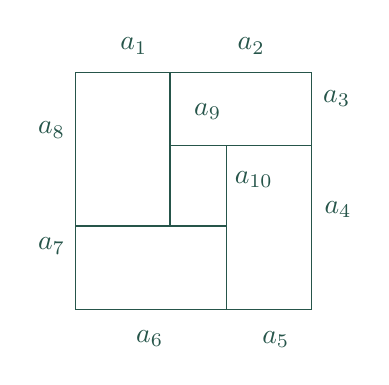
\begin{tikzpicture}[scale=0.6,thachthuctoanhoc]
			\draw  (0.,0.)-- (5.,0.);
			\draw  (0.,5.)-- (5.,5.);
			\draw  (5.,5.)-- (5.,0.);
			\draw  (0.,5.)-- (0.,0.);
			\draw  (2.,5.)-- (2.,1.76);
			\draw  (2.,1.76)-- (0.,1.76);
			\draw  (2.,3.46)-- (5.,3.46);
			\draw  (3.2,3.46)-- (3.2,0.);
			\draw  (2.,1.76)-- (3.2,1.76);
			\draw (0.7411478095238109,5.945053904761909) node[anchor=north west] {$a_1$};
			\draw (3.225934666666671,5.945053904761909) node[anchor=north west] {$a_2$};
			\draw (5.035841142857149,4.840704190476194) node[anchor=north west] {$a_3$};
			\draw (5.06651752380953,2.4786228571428586) node[anchor=north west] {$a_4$};
			\draw (3.7474331428571475,-0.2619525714285716) node[anchor=north west] {$a_5$};
			\draw (1.0785880000000017,-0.24233053333333336) node[anchor=north west] {$a_6$};
			\draw (-1,1.7117133333333343) node[anchor=north west] {$a_7$};
			\draw (-1,4.165823809523812) node[anchor=north west] {$a_8$};
			\draw (2.305643238095241,4.564616761904765) node[anchor=north west] {$a_9$};
			\draw (3.1645819047619086,3.1228268571428592) node[anchor=north west] {$a_{10}$};
		\end{tikzpicture}
		\caption{\small\textit{\color{thachthuctoanhoc}Hình $1$}}
		\vspace*{-15pt}
	\end{figure}
	Ta có $\left\{ {{a_1};{a_2}; \ldots ;{a_{10}}} \right\} = \left\{ {1;2; \ldots ;10} \right\},$ và
	\begin{align*}
		n = {a_1} + {a_2} = {a_3} + {a_4} = {a_5} + {a_6} = {a_7} + {a_8}.
	\end{align*}
	Do đó
	\begin{align*}
		4n &= {a_1} + {a_2} + {a_3} + {a_4} + {a_5} + {a_6} + {a_7} + {a_8} \\
		&\le 3 + 4 + 5 + 6 + 7 + 8 + 9 + 10 = 52;
	\end{align*}
	suy ra, $n \le 13$. Mà theo giả thiết, $n \ge 13$, nên $n = 13$.
	\vskip 0.05cm
	Như vậy, với $n \ge 13$, ta có thể phân chia hình vuông cạnh $n$ thành năm hình chữ nhật, thỏa mãn các yêu cầu của đề bài, chỉ khi $n = 13$.
	\vskip 0.05cm
	Với $n = 13$, phân chia được thể hiện ở Hình $2$ dưới đây thỏa mãn các yêu cầu của đề bài.
	\begin{figure}[H]
		\vspace*{-15pt}
		\centering
		\captionsetup{labelformat= empty, justification=centering}
		\begin{tikzpicture}[scale=0.25,thachthuctoanhoc]
			\draw  (0.,0.)-- (12.902720021180311,0.);
			\draw  (0.,12.902720021180311)-- (12.902720021180311,12.902720021180311);
			\draw  (12.902720021180311,12.902720021180311)-- (12.902720021180311,0.);
			\draw  (0.,12.902720021180311)-- (0.,0.);
			\draw  (9.025004744255101,12.902720021180313)-- (9.025004744255101,6.);
			\draw  (9.025004744255101,6.)-- (0.,6.);
			\draw  (9.025004744255101,8.033375486746607)-- (12.902720021180311,8.033375486746607);
			\draw  (10.,8.033375486746607)-- (10.,0.);
			\draw  (9.025004744255101,6.)-- (10.,6.);
			\draw (4.231659743459114,14.7289269960977) node[anchor=north west] {$9$};
			\draw (10.574639348977636,14.751598908646) node[anchor=north west] {$4$};
			\draw (13.261077770138423,11.311830988972293) node[anchor=north west] {$5$};
			\draw (8.68156796848920555,9.7755594148325) node[anchor=north west] {$1$};
			\draw (10.126899612117505,7.6552898046145526) node[anchor=north west] {$2$};
			\draw (13.186454480661734,4.595734936070321) node[anchor=north west] {$8$};
			\draw (11.246248954267832,-0.25477887991443754) node[anchor=north west] {$3$};
			\draw (4.679399480319246,-0.25477887991443754) node[anchor=north west] {$10$};
			\draw (-1.58427239409557028,3.625632172873369) node[anchor=north west] {$6$};
			\draw (-1.59919705199090798,10.043235067868588) node[anchor=north west] {$7$};
		\end{tikzpicture}
		\caption{\small\textit{\color{thachthuctoanhoc}Hình $2$}}
		\vspace*{-15pt}
	\end{figure}
	Vậy, nếu $n = 13$ thì câu trả lời cho câu hỏi đặt ra ở bài toán là ``\textit{có thể}"; nếu $n > 13$ thì câu trả lời là ``\textit{không thể}".
	\vskip 0.05cm
	\textbf{\color{thachthuctoanhoc}Bình luận và Nhận xét}
	\vskip 0.05cm
	Trong số các lời giải Tạp chí nhận được từ bạn đọc, rất tiếc, có một lời giải sai (do người giải bài đã mắc khá nhiều lỗi logic trong các lập luận) và một lời giải không được chấp nhận là lời giải hoàn chỉnh, do có câu trả lời không chính xác cho câu hỏi của bài toán và mắc một số lỗi ``chính tả" trong các diễn đạt toán học.
	\vskip 0.05cm
	Xin lưu ý, ``${a_1},{a_2}, \ldots ,{a_{10}} \in \left\{ {1;2; \ldots ;10} \right\}$" và ``$\left\{ {{a_1},{a_2}, \ldots ,{a_{10}}} \right\} = \left\{ {1;2; \ldots ;10} \right\}$" là hai khẳng định hoàn toàn khác nhau.
	\vskip 0.05cm
	\hfill \textbf{\color{thachthuctoanhoc}Lê Huy}
	\vskip 0.05cm
	{\color{thachthuctoanhoc}{\usefont{T5}{qag}{b}{n} P667.}}
	(Mức $A$) Chứng minh rằng
	\begin{align*}
		8(x+y-1)^2-9xy(x+y-1)+xy\ge0
	\end{align*}
	với mọi $x,y\in[0;1]$. 
	\vskip 0.05cm
	\textbf{\color{thachthuctoanhoc}Lời giải} (\textit{của người chấm bài})\textbf{\color{thachthuctoanhoc}.}
	\vskip 0.05cm
	Đặt $a = \dfrac{x + y}{2}$; khi đó, bất đẳng thức của đề bài trở thành
	\begin{align*}
		4{\left( {2a - 1} \right)^2} + xy\left( {5 - 9a} \right) \ge 0. \tag{$1$}
	\end{align*}
	Vì $x, y \in [0; 1]$ nên $a \in [0; 1]$.
	\vskip 0.05cm
	Nếu  $0 \le a \le \dfrac{5}{9}$ thì bất đẳng thức ($1$) hiển nhiên đúng.
	\vskip 0.05cm
	Xét $\dfrac{5}{9} < a \le 1$.
	\vskip 0.05cm  
	Khi đó, $5 - 9a < 0.$ \hfill ($2$)
	\vskip 0.05cm
	Theo bất đẳng thức trung bình cộng -- trung bình nhân, ta có:
	\begin{align*}
		{a^2} = {\left( {\dfrac{{x + y}}{2}} \right)^2} \ge xy. \tag{$3$}
	\end{align*}
	Từ ($2$) và ($3$), suy ra
	\begin{align*}
			&4{\left( {2a - 1} \right)^2} + xy\left( {5 - 9a} \right) \\
			\ge \,&4{\left( {2a - 1} \right)^2} + {a^2}\left( {5 - 9a} \right)\\
		 = \,&4 - 16a + 21{a^2} - 9{a^3}\\
		= \,&\left( {1 - a} \right){\left( {2 - 3a} \right)^2} \ge 0\left( {{\text{do }}a \le 1} \right).
	\end{align*}
	Bất đẳng thức ($1$) được chứng minh; và vì thế, bất đẳng thức của bài ra được chứng minh.
	\vskip 0.05cm
	\textbf{\color{thachthuctoanhoc}Bình luận và Nhận xét}
	\vskip 0.05cm
	$\pmb{1.}$ Dễ dàng chứng minh được rằng, dấu ``$=$" ở bất đẳng thức của đề bài xảy ra khi và chỉ khi
	\begin{align*}
		\left( {x,y} \right) \in \left\{ {\left( {0,1} \right),\left( {1,0} \right),\left( {1,1} \right),\left( {\dfrac{2}{3},\dfrac{2}{3}} \right)} \right\}.
	\end{align*}
	$\pmb{2.}$ Bằng cách đặt $z = 2 - x - y$, có thể biến đổi bất đẳng thức của đề bài về bất đẳng thức Schur bậc ba
	\begin{align*}
		xyz \ge \left( {x + y - z} \right)\left( {y + z - x} \right)\left( {z + x - y} \right).
	\end{align*}
	Vì thế, có thể nói, bất đẳng thức của bài ra là một trường hợp đặc biệt của bất đẳng thức vừa nêu trên, khi $z = 2 - x - y$.
	\vskip 0.05cm
	$\pmb{3.}$ Trong số các lời giải Tạp chí đã nhận được từ bạn đọc, rất tiếc, có một số lời giải sai, do người giải bài đã nhầm lẫn chiều của các bất đẳng thức, hoặc thực hiện sai một số tính toán.
	\vskip 0.05cm
	\hfill \textbf{\color{thachthuctoanhoc}Võ Quốc Bá Cẩn}
	\vskip 0.05cm
	{\color{thachthuctoanhoc}{\usefont{T5}{qag}{b}{n} P668.}}
	(Mức $A$) Cho số nguyên $n\ge2$. Có $n$ con ếch nằm trên một trục số, tại $n$ điểm tuỳ ý, thuộc tập $2n$ điểm $1,2,\ldots,2n$. Vào cùng một thời điểm, mỗi con ếch đều nhảy đến một trong số $n$ điểm còn lại, thuộc tập $2n$ điểm vừa nêu, sao cho không có hai con nào cùng nhảy tới một điểm. Chứng minh rằng
	\vskip 0.05cm
	$a)$ Tổng khoảng cách $n$ con ếch đã nhảy không vượt quá $n^2$. 
	\vskip 0.05cm
	$b)$ Tồn tại một phương án nhảy của $n$ con ếch, sao cho tổng khoảng cách chúng đã nhảy đúng bằng $n^2$. 
	\vskip 0.05cm
	\textbf{\color{thachthuctoanhoc}Lời giải} (\textit{dựa theo lời giải của tác giả bài toán}).
	\vskip 0.05cm
	Lần lượt, theo thứ tự từ bé đến lớn, ký hiệu ${a_1},{a_2}, \ldots ,{a_n}$  là các điểm mà n con ếch nằm ở thời điểm ban đầu.
	\vskip 0.05cm
	Với mỗi $i = 1, 2, \ldots, n$, gọi con ếch nằm ở điểm  $a_i$ là con ếch thứ $i$.
	\vskip 0.05cm
	Với mỗi $i = 1, 2, \ldots, n$, ký hiệu $b_i$  là điểm con ếch thứ $i$ nhảy đến.
	\vskip 0.05cm
	Theo giả thiết của bài ra,
	\begin{align*}
		&\left\{ {{a_1};{a_2}; \ldots ;{a_n};{b_1};{b_2}; \ldots ;{b_n}} \right\} \\
		= \,&\left\{ {1;2; \cdots ;2n} \right\}. \tag{$1$}
	\end{align*}
	Với mỗi $i = 1, 2, \ldots, n$, khoảng cách con ếch thứ $i$ đã nhảy là $\left| {{a_i} - {b_i}} \right|.$
	\vskip 0.05cm 
	Ký hiệu $S$ là tổng khoảng cách $n$ con ếch đã nhảy. Do với mọi $i = 1, 2, \ldots , n$,
	\begin{align*}
		\left| {{a_i} - {b_i}} \right| = \max \left\{ {{a_i},{b_i}} \right\} - \min \left\{ {{a_i},{b_i}} \right\},
	\end{align*}
	nên
	\begin{align*}
		S = \sum\limits_{i = 1}^n {\max \left\{ {{a_i},{b_i}} \right\}}  - \sum\limits_{i = 1}^n {\min \left\{ {{a_i},{b_i}} \right\}}  \tag{$2$}
	\end{align*}
	$a)$ Do ($1$) nên
	\begin{align*}
		\sum\limits_{i = 1}^n {\max \left\{ {{a_i},{b_i}} \right\}}  &\!\le\! \left( {n \!+\! 1} \right) \!+\! \left( {n \!+\! 2} \right) \!+\!  \cdots  \!+\! 2n \\[-1.2ex]
		&= {n^2} + \sum\limits_{i = 1}^n i,  \tag{$3$}\\[-1ex]
	\sum\limits_{i = 1}^n {\min \left\{ {{a_i},{b_i}} \right\}}  &\ge \sum\limits_{i = 1}^n i. \tag{$4$}
\end{align*}
	Từ ($2$), ($3$) và ($4$), suy ra
	\begin{align*}
		S \le \left( {{n^2} + \sum\limits_{i = 1}^n i } \right) - \sum\limits_{i = 1}^n i  = {n^2}.
	\end{align*}
	Ta có điều phải chứng minh theo yêu cầu đề bài.
	\vskip 0.05cm
	$b)$ Lần lượt, theo thứ tự từ lớn đến bé, ký hiệu ${c_1},{c_2}, \ldots ,{c_n}$  là các phần tử của tập hợp
	\begin{align*}
		\left\{ {1;2; \ldots ;2n} \right\}\backslash \left\{ {{a_1};{a_2}; \ldots ;{a_n}} \right\}.
	\end{align*}
	Xảy ra hai trường hợp sau:
	\vskip 0.05cm
	$\diamond$ \textit{Trường hợp} $1$:
	\vskip 0.05cm  
	Khi đó, $\left\{ {{c_1},{c_2}, \ldots ,{c_n}} \right\} \!=\! \left\{ {n \!+\! 1;n \!+\! 2; \ldots ;2n} \right\}\!.$  Do đó, với mọi $i = 1, 2, \ldots, n$,
	\begin{align*}
		\max \!\left\{\! {{a_i},{c_i}} \!\right\} \!=\! {c_i} \!\ge\! n \!+\! 1, \min\! \left\{\! {{a_i},{c_i}} \!\right\} \!=\! {a_i} \!\le\! n.
	\end{align*}
	$\diamond$ \textit{Trường hợp} $2$: Tồn tại $k \in \mathbb{N^*}$  sao cho  $1 \le {a_1} <  \cdots  < {a_k} \le n < {a_{k + 1}} <  \cdots  < {a_n} \le 2n.$ 
	\vskip 0.05cm
	Khi đó, ${c_1} >  \cdots  > {c_k} \ge n + 1 > {c_{k + 1}} >  \cdots  > {c_n} \ge 1.$ 
	\vskip 0.05cm
	Do đó, với mọi $i = 1, 2, \ldots , k$,
	\begin{align*}
		\max \!\left\{\! {{a_i},{c_i}} \!\right\} \!=\! {c_i} \!\ge\! n \!+\! 1, \min\! \left\{ \!{{a_i},{c_i}} \!\right\} \!=\! {a_i} \!\le\! n.
	\end{align*}
	và với mọi $i = k + 1, \ldots , n$,
	\begin{align*}
		\max\! \left\{\! {{a_i},{c_i}} \!\right\} \!=\! {a_i} \!\ge\! n \!+\! 1, \min\! \left\{\! {{a_i},{c_i}} \!\right\} \!=\! {c_i} \!\le\! n.
	\end{align*}
	Từ kết quả xét hai trường hợp trên, suy ra, ta luôn có
	\begin{align*}
		\max \!\left\{\! {{a_i},{c_i}} \!\right\} \!\ge\! n \!+\! 1,\min\! \left\{\! {{a_i},{c_i}} \!\right\} \!\le\! n, \tag{$5$}
	\end{align*}
	với mọi $i = 1, 2, \ldots, n$.
	\vskip 0.05cm
	Xét phương án nhảy như sau của $n$ con ếch: Với mỗi $i = 1, 2, \ldots, n$, $b_i = c_i$.
	\vskip 0.05cm  
	Khi đó, theo ($5$),
	\begin{align*}
		\max \!\left\{\! {{a_i},{b_i}} \!\right\} \!\ge\! n \!+\! 1,\min\! \left\{\! {{a_i},{b_i}} \!\right\} \!\le\! n,
	\end{align*}
	với mọi $i = 1, 2, \ldots , n$.
	\vskip 0.05cm
	Do đó, với lưu ý tới ($1$), ta có:
	\begin{align*}
		\sum\limits_{i = 1}^n {\max \left\{ {{a_i},{b_i}} \right\}}  &= \left( {n \!+\! 1} \right) \!+\! \left( {n \!+\! 2} \right) \!+\!  \cdots \! +\! 2n \\[-1.2ex]
		&= {n^2} + \sum\limits_{i = 1}^n i\\[-1.2ex]
		\sum\limits_{i = 1}^n {\min \left\{ {{a_i},{b_i}} \right\}}  &= \sum\limits_{i = 1}^n i.
	\end{align*}
	Vì thế, theo ($2$), $S = n^2$.
	\vskip 0.05cm  
	Ta có điều phải chứng minh theo yêu cầu đề bài.
	\vskip 0.05cm
	\textbf{\color{thachthuctoanhoc}Bình luận và Nhận xét}
	\vskip 0.05cm
	Tạp chí đã nhận được hai lời giải, từ bạn đọc; trong đó, rất tiếc, có một lời giải sai ở ý $b)$, do người giải bài, khi xây dựng phương án nhảy của $n$ con ếch, đã áp đặt vị trí ban đầu của chúng là $n$ điểm $1, 2, \ldots, n$.
	\vskip 0.05cm
	\hfill	\textbf{\color{thachthuctoanhoc}Nguyễn Khắc Minh}
	\vskip 0.05cm
	{\color{thachthuctoanhoc}{\usefont{T5}{qag}{b}{n} P669.}}
	(Mức $A$) Cho tam giác nhọn $ABC$, với $AB<AC$, nội tiếp đường tròn $(O)$. Gọi $M,N$ tương ứng là trung điểm của các cung $BC$ lớn và cung $BC$ nhỏ. Trên đường thẳng $AN$, lấy điểm $D$ sao cho $D$ nằm trong tam giác $ABC$ và không trùng với tâm đường tròn nội tiếp tam giác ấy. Trên đoạn thẳng $MD$, lấy điểm $T$ sao cho $\angle{MBT}=\angle{DCB}$. Chứng minh rằng trực tâm của tam giác $TND$ nằm trên đường thẳng $BC$.
	\vskip 0.05cm
	\textbf{\color{thachthuctoanhoc}Lời giải} (\textit{của người chấm bài}).
	\begin{figure}[H]
		\vspace*{-10pt}
		\centering
		\captionsetup{labelformat= empty, justification=centering}
		\definecolor{ffqqqq}{rgb}{1.,0.,0.}
		\definecolor{qqwuqq}{rgb}{0.,0.39215686274509803,0.}
		\definecolor{xdxdff}{rgb}{0.49019607843137253,0.49019607843137253,1.}
		\definecolor{uuuuuu}{rgb}{0.26666666666666666,0.26666666666666666,0.26666666666666666}
		\definecolor{qqqqff}{rgb}{0.,0.,1.}
		\begin{tikzpicture}[scale=0.32,thachthuctoanhoc]
			\draw [shift={(10.,-2.)},pattern color=qqwuqq,fill=qqwuqq,fill opacity=0.10000000149011612] (0,0) -- (166.8046508068974:0.88) arc (166.8046508068974:180.:0.88) -- cycle;
			\draw [shift={(0.,-2.)},pattern color=qqwuqq,fill=qqwuqq,fill opacity=0.10000000149011612] (0,0) -- (44.4249154392908:0.88) arc (44.4249154392908:57.6202646323934:0.88) -- cycle;
			\draw[pattern color=qqwuqq,fill=qqwuqq,fill opacity=0.10000000149011612] (3.028672358412081,-4.746051562850727) -- (3.0941777880108416,-4.441898577178908) -- (2.790024802339022,-4.376393147580148) -- (2.7245193727402617,-4.680546133251967) -- cycle; 
			\draw [shift={(4.185301543683374,2.1021169441445613)},pattern color=qqwuqq,fill=qqwuqq,fill opacity=0.10000000149011612] (0,0) -- (-135.5750845607092:0.66) arc (-135.5750845607092:-102.15414161359068:0.66) -- cycle;
			\draw [shift={(10.,-2.)},pattern color=qqwuqq,fill=qqwuqq,fill opacity=0.10000000149011612] (0,0) -- (166.8046508068974:0.66) arc (166.8046508068974:200.22559375401596:0.66) -- cycle;
			\draw [shift={(2.7245193727402617,-4.680546133251967)},pattern color=qqwuqq,fill=qqwuqq,fill opacity=0.10000000149011612] (0,0) -- (20.225593754015947:0.66) arc (20.225593754015947:77.84585838640933:0.66) -- cycle;
			\draw [shift={(2.7245193727402617,-4.680546133251967)},pattern color=qqwuqq,fill=qqwuqq,fill opacity=0.10000000149011612] (0,0) -- (77.84585838640933:0.44) arc (77.84585838640933:135.4661230188027:0.44) -- cycle;
			\draw[pattern color=ffqqqq,fill=ffqqqq,fill opacity=0.10000000149011612] (2.662862274480868,1.6530470327261946) -- (2.7508851876612797,1.354631271153127) -- (3.049300949234347,1.442654184333539) -- (2.961278036053935,1.7410699459066064) -- cycle; 
			\draw  (2.,5.)-- (0.,-2.);
			\draw  (0.,-2.)-- (10.,-2.);
			\draw  (10.,-2.)-- (2.,5.);
			\draw  (5.,0.35714285714285715) circle (5.527759261127387cm);
			\draw  (5.,-5.17061640398453)-- (2.,5.);
			\draw  (3.6238019594012094,-0.505022281702721)-- (10.,-2.);
			\draw  (5.,5.884902118270244)-- (3.6238019594012094,-0.505022281702721);
			\draw  (5.,5.884902118270244)-- (0.,-2.);
			\draw  (4.185301543683374,2.1021169441445613)-- (0.,-2.);
			\draw (1.3538,6.796) node[anchor=north west] {$A$};
			\draw (-0.64,-2.228) node[anchor=north west] {$B$};
			\draw (10.008,-1.728) node[anchor=north west] {$C$};
			\draw (4.64,7.242) node[anchor=north west] {$M$};
			\draw (4.75,-4.984) node[anchor=north west] {$N$};
			\draw (4.992,0.626) node[anchor=north west] {$O$};
			\draw (3.1,-0.21) node[anchor=north west] {$D$};
			\draw (3.7266,2.804) node[anchor=north west] {$T$};
			\draw (2.0286,-4.722) node[anchor=north west] {$K$};
			\draw  (3.6238019594012094,-0.505022281702721)-- (2.7245193727402617,-4.680546133251967);
			\draw  (4.185301543683374,2.1021169441445613)-- (5.,-5.17061640398453);
			\draw  (4.185301543683374,2.1021169441445613)-- (-9.72171775070981,-2.);
			\draw  (5.,-5.17061640398453)-- (5.,5.884902118270244);
			\draw (-10.43,-1.954) node[anchor=north west] {$H$};
			\draw  (-9.72171775070981,-2.)-- (5.,-5.17061640398453);
			\draw  (-9.72171775070981,-2.)-- (0.,-2.);
			\draw  (2.7245193727402617,-4.680546133251967)-- (10.,-2.);
			\draw  (2.7245193727402617,-4.680546133251967)-- (0.,-2.);
			\draw  (5.,-5.17061640398453)-- (10.,-2.);
			\draw [shift={(4.185301543683374,2.1021169441445613)},color=qqwuqq] (-135.5750845607092:0.66) arc (-135.5750845607092:-102.15414161359068:0.66);
			\draw [shift={(4.185301543683374,2.1021169441445613)},color=qqwuqq] (-135.5750845607092:0.55) arc (-135.5750845607092:-102.15414161359068:0.55);
			\draw [shift={(10.,-2.)},color=qqwuqq] (166.8046508068974:0.66) arc (166.8046508068974:200.22559375401596:0.66);
			\draw [shift={(10.,-2.)},color=qqwuqq] (166.8046508068974:0.55) arc (166.8046508068974:200.22559375401596:0.55);
			\draw [shift={(2.7245193727402617,-4.680546133251967)},color=qqwuqq] (20.225593754015947:0.66) arc (20.225593754015947:77.84585838640933:0.66);
			\draw[color=qqwuqq] (3.113938829900631,-4.232005737763528) -- (3.20047648704738,-4.132330094321653);
			\draw [shift={(2.7245193727402617,-4.680546133251967)},color=qqwuqq] (77.84585838640933:0.44) arc (77.84585838640933:135.4661230188027:0.44);
			\draw[color=qqwuqq] (2.6173217256447794,-4.322238075210854) -- (2.5794872619640197,-4.195776407666933);
			\draw  (-9.72171775070981,-2.)-- (3.6238019594012094,-0.505022281702721);
			\draw  (0.,-2.)-- (5.,-5.17061640398453);
			\draw [fill=white] (2.,5.) circle (1.5pt);
			\draw [fill=white] (0.,-2.) circle (1.5pt);
			\draw [fill=white] (10.,-2.) circle (1.5pt);
			\draw [fill=white] (5.,0.35714285714285715) circle (1.5pt);
			\draw [fill=white] (5.,-5.17061640398453) circle (1.5pt);
			\draw [fill=white] (5.,5.884902118270244) circle (1.5pt);
			\draw [fill=white] (3.6238019594012094,-0.505022281702721) circle (1.5pt);
			\draw [fill=white] (0.,-2.) circle (1.5pt);
			\draw [fill=white] (0.,-2.) circle (1.5pt);
			\draw [fill=white] (4.185301543683374,2.1021169441445613) circle (1.5pt);
			\draw [fill=white] (5.,5.884902118270244) circle (1.5pt);
			\draw [fill=white] (2.7245193727402617,-4.680546133251967) circle (1.5pt);
			\draw [fill=white] (-9.72171775070981,-2.) circle (1.5pt);
		\end{tikzpicture}
		\vspace*{-20pt}
	\end{figure}
	Gọi $K$ là giao điểm thứ hai, khác $M$, của $MD$ và $(O)$.
	\vskip 0.05cm
	Do $M$ là điểm chính giữa cung $BAC$ nên
	\begin{align*}
		\angle BKT \!=\! \angle BKM \!=\! \angle MKC \!=\! \angle DKC. \tag{$1$}
	\end{align*}
	Do $BKCM$ là tứ giác nội tiếp, nên $\angle BMK = \angle BCK$; kết hợp với giả thiết $\angle MBT = \angle DCB,$  suy ra
	\begin{align*}
		\angle BTK &= \angle MBT + \angle BMK \\
		&= \angle DCB + \angle BCK = \angle DCK. \tag{$2$}
	\end{align*}
	Từ ($1$) và ($2$), suy ra $\Delta BKT \sim  \Delta DKC$; do đó
	\begin{align*}
		\dfrac{{KB}}{{KT}} = \dfrac{{KD}}{{KC}} \tag{$3$}
	\end{align*}
	Gọi $H$ là giao điểm của $NK$ và $BC$.
	\vskip 0.05cm
	Từ giả thiết về vị trí của các điểm $M$, $N$, suy ra $MN$ là đường kính của $(O)$. Do đó, $KN \bot KM$; mà $KM$ là phân giác trong của góc $BKC$ (vì $M$ là điểm chính giữa cung $BAC$), nên $KN$ là phân giác ngoài của góc $BKC$. Suy ra, $\angle NKC = \angle BKH$. \hfill ($4$)
	\vskip 0.05cm 
	Vì $BKNC$ là tứ giác nội tiếp, nên $\angle KNC = \angle KBH.$ \hfill ($5$)
	\vskip 0.05cm
	Từ ($4$) và ($5$), suy ra $\Delta NKC \sim \Delta BKH$; do đó
	\begin{align*}
		\dfrac{{KC}}{{KN}} = \dfrac{{KH}}{{KB}}. \tag{$6$}
	\end{align*}
	Từ ($3$) và ($6$), suy ra
	\begin{align*}
		\dfrac{{KH}}{{KT}} = \dfrac{{KH}}{{KB}} \cdot \dfrac{{KB}}{{KT}} = \dfrac{{KC}}{{KN}} \cdot \dfrac{{KD}}{{KC}} = \dfrac{{KD}}{{KN}}.
	\end{align*}
	Mà  $\angle TKH = \angle NKD = {90^{\rm{o}}}$ (do $KN \bot KM$, theo chứng minh trên), nên $\Delta KHT \sim  \Delta KDN$. Suy ra
	\begin{align*}
		\angle THK = \angle NDK = {90^{\rm{o}}} - \angle KND.
	\end{align*}
	Do đó
	\begin{align*}
		\angle THN + \angle HND = \angle THK + \angle KND = {90^\circ}.
	\end{align*}
	Suy ra, $TH \bot ND$. Mà $NH \bot TD$ (do $KN \bot KM$, theo chứng minh trên), nên $H$ là trực tâm của tam giác $TND$. Vì vậy, trực tâm của tam giác $TND$ nằm trên đường thẳng $BC$.
	\vskip 0.05cm
	Ta có điều phải chứng minh theo yêu cầu đề bài.
	\vskip 0.05cm
	\textbf{\color{thachthuctoanhoc}Bình luận và Nhận xét}
	\vskip 0.05cm
	$\pmb{1.}$ Để chứng minh điểm $H$ (được định nghĩa trong lời giải trên) là trực tâm của tam giác $TND$, ngoài cách đã trình bày ở lời giải trên, còn có thể chứng minh bằng cách chứng minh và sử dụng kết quả sau:
	\vskip 0.05cm
	``\textit{Cho tam giác $ABC$, với đường cao $AD$ ($D \in BC$). Khi đó, điểm $H \in AD$ là trực tâm của tam giác đã cho khi và chỉ khi  $\overline {DB}  \cdot \overline {DC}  = \overline {HA}  \cdot \overline {HD} .$}"
	\vskip 0.05cm
	$\pmb{2.}$ Trong số các lời giải Tạp chí đã nhận được từ bạn đọc, có một lời giải không được chấp nhận là lời giải đúng, do người giải bài đã sử dụng chưa đúng kết quả vừa nêu ở mục $1$ trên đây.
	\begin{flushright}
		\textbf{\color{thachthuctoanhoc}Hạ Vũ Anh}
	\end{flushright}
	{\color{thachthuctoanhoc}{\usefont{T5}{qag}{b}{n} P670.}}
	(Mức $A$) Hỏi, có thể chọn được tối đa bao nhiêu điểm nguyên trong mặt phẳng toạ độ, sao cho đoạn thẳng nối hai điểm bất kỳ trong chúng chứa đúng $2022$ điểm nguyên?
	\vskip 0.05cm
	(Trong mặt phẳng toạ độ, một điểm được gọi là {\it điểm nguyên}, nếu cả hoành độ và tung độ của nó đều là các số nguyên.)
	\vskip 0.05cm
	\textbf{\color{thachthuctoanhoc}Lời giải} (\textit{của người chấm bài})\textbf{\color{thachthuctoanhoc}.}
	\vskip 0.05cm
	Trong phần trình bày dưới đây, $\gcd(a, b)$ ký hiệu ước chung lớn nhất của hai số nguyên $a, b$.\vskip 0.05cm
	Trước hết, ta nhắc lại (có chứng minh) kết quả quen biết sau:
	\vskip 0.05cm
	\textbf{Bổ đề.} Trong mặt phẳng tọa độ $Oxy$, cho hai điểm nguyên phân biệt $A(a, b)$ và $B(u, v)$. Khi đó, số điểm nguyên thuộc đoạn thẳng $AB$ bằng $\gcd(a - u, b - v) + 1$.
	\vskip 0.05cm
	\textit{Chứng minh.}
	\vskip 0.05cm
	Không mất tính tổng quát, giả sử $b \ge  v$.
	\vskip 0.05cm
	Xét phép tịnh tiến theo vectơ $\overrightarrow{BO}$. Qua phép tịnh tiến này, điểm $A$ biến thành điểm $A'\left( {a - u,b - v} \right),$  và điểm $B$ biến thành gốc tọa độ $O$. Dễ thấy, số điểm nguyên thuộc đoạn thẳng $AB$ bằng số điểm nguyên thuộc đoạn thẳng $OA'$.
	\vskip 0.05cm 
	Gọi $s$ là số điểm nguyên thuộc đoạn thẳng $OA'$.
	\vskip 0.05cm
	Do $b \ge  v$ nên xảy ra hai trường hợp sau:
	\vskip 0.05cm
	$\diamond$ \textit{Trường hợp} $1$: $b = v$.
	\vskip 0.05cm
	Khi đó, $A'$  là điểm nằm trên trục hoành, và có hoành độ là $a - u$. Vì vậy
	\begin{align*}
		s = (a - u) + 1 &= \gcd(a - u, 0) + 1 \\
		&= \gcd(a - u, b - v) + 1.
	\end{align*}
	$\diamond$ \textit{Trường hợp} $2$: $b > v$.
	\vskip 0.05cm
	Đặt $d = \gcd(a - u, b - v)$.
	\vskip 0.05cm
	Khi đó, tồn tại $c\in \mathbb{Z}$  và $k \in \mathbb{N^*}$  nguyên tố cùng nhau, sao cho
	\begin{align*}
		a - u = cd \text{ và } b - v = kd.
	\end{align*}
	Xảy ra hai trường hợp sau:
	\vskip 0.05cm
	$+$ \textit{Trường hợp} $2.1$: $a = u$.
	\vskip 0.05cm
	Khi đó, $A'$  là điểm nằm trên trục tung, và có tung độ là $b - v$. Vì thế
	\begin{align*}
		s = (b - v) + 1 &= \gcd(0, b - v) + 1 \\
		&= \gcd(a - u, b - v) + 1.
	\end{align*}
	$+$ \textit{Trường hợp} $2.2$: $a \ne u$.
	\vskip 0.05cm
	Khi đó, $c \ne 0$; do đó, đường thẳng $OA'$  có phương trình:
	\begin{align*}
		y = \frac{k}{c}x.
	\end{align*}
	Vì thế, với điểm $M\left( {{x_M},{y_M}} \right)$  tùy ý thuộc đoạn thẳng $OA'$,  ta có $0 \le {y_M} \le kd,$  và
	\begin{align*}
		{y_M} = \frac{k}{c}{x_M}.
	\end{align*}
	Từ đó, do $\gcd(c, k) = 1$, suy ra, điểm  $M\left( {{x_M},{y_M}} \right)$ thuộc đoạn thẳng  $OA'$ là điểm nguyên khi và chỉ khi $x_m = hc$,  với $h$ là số tự nhiên thỏa mãn $0 \le h \le d$. Vì vậy
	\begin{align*}
		s = d + 1 = \gcd(a - u, b - v) + 1.
	\end{align*}
	Kết quả xét các trường hợp nêu trên cho ta điều phải chứng minh theo yêu cầu của Bổ đề.
	\vskip 0.05cm
	\textit{Trở lại bài toán.}
	\vskip 0.05cm
	Xét số nguyên dương $n$, mà với nó, tồn tại $n$ điểm phân biệt  ${A_1}\left( {{x_1},{y_1}} \right),$ ${A_2}\left( {{x_2},{y_2}} \right), \ldots ,$ ${A_n}\left( {{x_n},{y_n}} \right)$, sao cho đoạn thẳng nối hai điểm bất kỳ trong chúng chứa đúng $2022$ điểm nguyên.
	\vskip 0.05cm
	Khi đó, theo Bổ đề,
	\begin{align*}
		\gcd \left( {{x_i} - {x_j},{y_i} - {y_j}} \right) = 2021, \tag{$1$}
	\end{align*}
	với mọi $i, j \in \{1; 2; \ldots ; n\}, i \ne j$.
	\vskip 0.05cm
	Với mỗi $i = 1, 2, \ldots , n$, gọi $r_i$  và $s_i$  tương ứng là số dư trong phép chia $x_i$  và $y_i$  cho $2$.
	\vskip 0.05cm
	Khi đó, do  ${r_i},{s_i} \in \left\{ {0;1} \right\}$ với mọi $i \in \{1; 2; \ldots ; n\}$, nên
	\begin{align*}
		\left( {{r_i},{s_i}} \right) \in \left\{ {\left( {0,0} \right);\left( {0,1} \right);\left( {1,0} \right);\left( {1,1} \right)} \right\}
	\end{align*}
	với mọi $i \in \{1; 2; \ldots ; n\}$.
	\vskip 0.05cm
	Vì thế, nếu $n \ge  5$ thì theo nguyên lý Dirichlet, tồn tại $p \ne q, p, q \in \{1; 2; \ldots ; n\}$, sao cho
	\begin{align*}
		\left( {{r_p},{s_p}} \right) = \left( {{r_q},{s_q}} \right).
	\end{align*}
	Nghĩa là, tồn tại $p \ne q, p, q \in \{1; 2; \ldots ; n\}$, sao cho 
	\begin{align*}
		{x_p} \equiv {x_q}\left( {\bmod 2} \right) \text{ và } {y_p} \equiv {y_q}\left( {\bmod 2} \right). \tag{$2$}
	\end{align*}
	Từ ($2$) và ($1$), suy ra
	\begin{align*}
		2\left| {\gcd \left( {{x_p} - {x_q},{y_p} - {y_q}} \right) = 2021,} \right.
	\end{align*}
	là điều vô lý. Vì vậy, $n \le 4$.
	\vskip 0.05cm
	Hơn nữa, bằng cách sử dụng Bổ đề, dễ dàng chứng minh được rằng, đoạn thẳng, nối hai điểm bất kỳ trong bốn điểm $A(0, 0),$ $B(0, 2021),$ $C(2021, 0),$ $D(2021, 2021)$, chứa đúng $2022$ điểm nguyên.
	\vskip 0.05cm
	Vậy, có thể chọn được tối đa bốn điểm nguyên trong mặt phẳng tọa độ, sao cho đoạn thẳng nối hai điểm bất kỳ trong chúng chứa đúng $2022$ điểm nguyên.
	\vskip 0.05cm
	\textbf{\color{thachthuctoanhoc}Bình luận và Nhận xét}
	\vskip 0.05cm
	$\pmb{1.}$ Lời giải trên cho thấy, bài đã ra là một khai thác nhẹ nhàng, thú vị đối với một kết quả cơ bản, quen biết về lưới nguyên trong mặt phẳng (Bổ đề trong lời giải trên).
	\vskip 0.05cm
	$\pmb{2.}$ Ở lời giải trên, thay $2021$ bởi $2n - 1$, $2022$ bởi $2n$, và $n$ bởi $m$, ta sẽ thu được một chứng minh cho khẳng định sau:
	\vskip 0.05cm
	``\textit{Với mọi số nguyên dương $n$, luôn chọn được tối đa bốn điểm nguyên trong mặt phẳng tọa độ, sao cho đoạn thẳng nối hai điểm bất kỳ trong chúng chứa đúng $2n$ điểm nguyên.}"
	\vskip 0.05cm
	$\pmb{3.}$ Trong số các lời giải Tạp chí nhận được từ bạn đọc, rất tiếc, có hai lời giải không được chấp nhận là lời giải hoàn chỉnh, do trong các lời giải đó có một số lập luận không chặt chẽ, thiếu chính xác.
	\begin{flushright}
		\textbf{\color{thachthuctoanhoc}Nguyễn Khắc Minh}
	\end{flushright}
\end{multicols}
{\centerline{\textbf{\color{thachthuctoanhoc}DANH SÁCH HỌC SINH CÓ LỜI GIẢI HOÀN CHỈNH}}}
\vskip 0.05cm
\textit{Trong các ngoặc đơn ở phần dưới đây, sau tên lớp là mã hiệu của các bài toán mà học sinh có lời giải hoàn chỉnh.}
\begin{multicols}{2}
	\textbf{\color{thachthuctoanhoc}KHỐI THCS}
	\vskip 0.05cm
	$\bullet$ Trường \textbf{\color{thachthuctoanhoc}THCS xã Pom Lót}, huyện Điện Biên, tỉnh Điện Biên: \textit{Nguyễn Ngọc Diệp} (lớp $9$D$3$; P$661$).
	\vskip 0.05cm
	\textbf{\color{thachthuctoanhoc}KHỐI THPT}
	\vskip 0.05cm
	$\bullet$ Trường \textbf{\color{thachthuctoanhoc}THPT chuyên Nguyễn Quang Diêu}, tỉnh Đồng Tháp: \textit{Lư Gia Hưng} (lớp $11$T$1$; P$662$), \textit{Đỗ Duy Quang} (lớp $11$T$1$; P$662$, P$664$).
	\vskip 0.05cm
	$\bullet$ Trường \textbf{\color{thachthuctoanhoc}THPT Chi Lăng}, tỉnh Gia Lai: \textit{Phan Trịnh Nguyên} (lớp $10$A$1$; P$661$).
	\vskip 0.05cm
	$\bullet$ Trường \textbf{\color{thachthuctoanhoc}THPT chuyên Hà Tĩnh}, tỉnh Hà Tĩnh: \textit{Trần Minh Hoàng} (lớp $10$T$1$; P$662$, P$663$, P$666$, P$667$, P$670$).
	\vskip 0.05cm
	$\bullet$ Trường \textbf{\color{thachthuctoanhoc}THPT chuyên Lê Hồng Phong}, tỉnh Nam Định: \textit{Nguyễn Hoàng Anh} (lớp $11$ Toán $2$; P$664$), \textit{Phùng Việt Cường} (lớp $11$ Toán $2$; P$661$, P$664$, P$666$), \textit{Nguyễn Đức Khải} (lớp $11$ Toán $2$; P$667$), \textit{Ninh Thị Mai Linh} (lớp $12$ Toán $1$; P$661$, P$664$), \textit{Đồng Đức Mạnh} (lớp $11$ Toán $1$; P$661$), \textit{Hà Thị Kim Oanh} (lớp $12$ Toán $1$; P$664$, P$669$), \textit{Nguyễn Xuân Tiến} (lớp $11$ Toán $2$; P$667$).
	\vskip 0.05cm
	$\bullet$ Trường \textbf{\color{thachthuctoanhoc}THPT chuyên Nguyễn Bỉnh Khiêm}, tỉnh Quảng Nam: \textit{Trịnh Quốc Khánh} (lớp $11$ chuyên Toán; P$669$).
	\vskip 0.05cm
	$\bullet$ Trường \textbf{\color{thachthuctoanhoc}THPT chuyên Tiền Giang}, tỉnh Tiền Giang: \textit{Trần Phúc Thịnh} (lớp $10$ Toán; P$661$), \textit{Nguyễn Hữu Trí} (lớp $10$ Toán; P$661$).
	\vskip 0.05cm
	$\bullet$ Trường \textbf{\color{thachthuctoanhoc}THPT chuyên Quốc học Huế}, tỉnh Thừa Thiên -- Huế: \textit{Nguyễn Thị Nhật Thảo} (lớp $11$ Toán $2$; P$661$), \textit{Trần Thị Thanh Thư} (lớp $12$ Toán $1$; P$661$), \textit{Đặng Quỳnh Bảo Uyên} (lớp $11$ Toán $2$; P$661$).
	\vskip 0.05cm
	$\bullet$ Trường \textbf{\color{thachthuctoanhoc}THPT chuyên Khoa học tự nhiên}, ĐH Khoa học tự nhiên -- ĐHQG Hà Nội: \textit{Vương Khánh Toàn} (lớp $10$A$1$ Toán; P$667$, P$668$, P$669$).
	\vskip 0.05cm
	$\bullet$ Trường \textbf{\color{thachthuctoanhoc}THPT chuyên Sư phạm}, ĐH Sư phạm Hà Nội: \textit{Hồ Trần Khánh Linh} (lớp $12$ Toán $2$; P$667$, P$669$).
\end{multicols}

%	\newpage 

%	\setcounter{figure}{0}
%	\thispagestyle{hoccungpinone}
\pagestyle{hoccungpi}
\everymath{\color{hoccungpi}}
\graphicspath{{../hoccungpi/pic/}}
%\blfootnote{$^{1}$\color{hoccungpi}Đại học Bách Khoa Hà Nội.}
\begingroup
\AddToShipoutPicture*{\put(0,616){\includegraphics[width=19.3cm]{../bannerhoccungpi}}}
\AddToShipoutPicture*{\put(90,550){\includegraphics[scale=1]{../tieude.pdf}}}
\centering
\endgroup
\vspace*{160pt}

\begin{multicols}{2}
	$\pmb{1.}$ \textbf{\color{hoccungpi}Đa thức và Hàm đa thức} 
	\vskip 0.1cm
	$\pmb{1.1.}$ \textbf{\color{hoccungpi}Đa thức.}
	Đa thức là một biểu thức đại số nhận được một cách hình thức từ các {\color{blue} biến số} và các {\color{blue} hệ số} thông qua các phép tính cộng, trừ và nhân. 
	\vskip 0.1cm
	Các hệ số là phần tử thuộc một tập hợp nào đó, thông thường là một tập hợp số (ví dụ $\mathbb {Z, Q, R, C}$) nhưng cũng có thể là một tập tổng quát hơn mà trên đó đã xác định các phép toán cộng, trừ, nhân. 
	\vskip 0.1cm
	Biến số là các ký tự hình thức (ví dụ $x,y,X,Y,...$) mà ta có thể thay thế chúng bằng những phần tử trong tập hợp chứa các hệ số hoặc một tập hợp lớn hơn mà trên đó cũng xác định các phép toán cộng, trừ và nhân.
	\vskip 0.1cm
	Đa thức một biến có thể được mô tả bằng biểu thức dạng
	\begin{align*}
		P(x)=a_0x^n+a_1x^{n-1}+\ldots+a_n.
	\end{align*}
	Như vậy thông tin về các đa thức một biến bao gồm hai loại: số tự nhiên $n$ được gọi là bậc của nó và các số (nguyên, hữu tỷ, thực hay phức) $a_0,a_1,\ldots, a_n$ -- các hệ số của nó. 
	\begin{tBox}
		Thông tin về đa thức một biến với bậc (không quá) $n$ là một dãy có thứ tự gồm $n+1$ {\em đơn vị thông tin}.
	\end{tBox}
	Dưới đây ta sẽ chỉ xét các {\color{blue} đa thức một biến} với hệ số nằm trong một tập số như $\mathbb{Q, R, C}$. 
	\vskip 0.1cm	
	$\pmb{1.2.}$ \textbf{\color{hoccungpi}Phép chia có dư.}  
	Đối với đa thức hệ số thực ta có thể thực hiện được phép chia có dư, tương tự như đối với các số nguyên. Cho các đa thức $P(x)$ và $Q(x)$ với $Q(x)\neq 0$, tồn tại duy nhất các đa thức $P_1(x)$ và $R(x)$ với $\deg R(x)<\deg Q(x)$ sao cho
	\begin{align*}
		P(x)= Q(x)P_1(x)+R(x).
	\end{align*}
	Ta nói đa thức $P(x)$ chia hết cho đa thức $Q(x)$ nếu $R(x)=0$.   
	\vskip 0.1cm
	\textbf{\color{hoccungpi}Chú ý}. Ta có thể thay thế điều kiện ``hệ số thực" bởi điều kiện ``hệ số phức" hay ``hệ số hữu tỷ". Nhưng ta không thể áp dụng với điều kiện ``hệ số nguyên". 
	\vskip 0.1cm
	Ví dụ, ta không thể thực hiện được phép chia có dư của đa thức $x^2+1$ cho đa thức $2x$ {\color{blue}trong tập hợp đa thức hệ số nguyên}!
	\vskip 0.1cm
	$\pmb{1.3.}$ \textbf{\color{hoccungpi}Hàm đa thức.}
	Xét các đa thức một biến với hệ số nằm trong một tập số. Khi đó, bằng cách thay thế biến số bằng các giá trị trong tập số đó ta thu được một hàm số. Hàm số thu được bằng cách này gọi là {\color{blue}hàm đa thức}. Chúng thường được mô tả ở dạng
	\begin{align*}
		y=P(x),
	\end{align*}
	trong đó $P(x)$ là một đa thức theo biến $x$.
	\vskip 0.1cm
	{\color{blue}Nguyên lý đồng nhất của Đại số học} nói rằng nếu hai hàm đa thức (trên tập số thực) bằng nhau tại mọi giá trị của biến số thì các đa thức xác định chúng bằng nhau. Nói cách khác, mỗi hàm đa thức được xác định bởi một đa thức duy nhất. 
	\vskip 0.1cm
	Ta chú ý rằng tính đúng đắn của nguyên lý này phụ thuộc vào miền giá trị của biến số (và hệ số). Ví dụ nguyên lý đồng nhất sai nếu xét đa thức trên tập các lớp đồng dư. 
	\vskip 0.1cm	
	$\pmb{1.4.}$ \textbf{\color{hoccungpi}Nghiệm của đa thức.}
	Nghiệm, hay còn gọi là không điểm, của một đa thức $P(x)$ là những giá trị của biến số $x$ mà tại đó $P(x)$ nhận giá trị $0$. Sử dụng phép chia có dư của $P(x)$ cho $x-a$ ta có
	\begin{align*}
		P(x)=(x-a)P_1(x)+P(a).
	\end{align*}
	Như vậy nếu $a$ là nghiệm của $P(x)$ thì $P(x)$ chia hết cho $x-a$. Từ đó ta kết luận một đa thức bậc $n$ {\color{blue} có không quá $n$ nghiệm}.
	\vskip 0.1cm
	{\color{blue} Định lý cơ bản của Đại số học} khẳng định mọi đa thức với hệ số phức với bậc lớn hoặc bằng $1$ luôn có nghiệm phức. 
	Từ đó suy ra, một đa thức bậc $n\geq 1$ luôn có thể viết được ở dạng
	\begin{align*}
		P(x)=a_0\prod_{i=1}^n(x-x_i), \quad x_i\in\mathbb C.
	\end{align*}
	Chú ý rằng các số (phức) $x_i$ có thể bằng nhau -- trong trường hợp đó ta nói $P(x)$ có {\em nghiệm bội}.
	\begin{tBox}
		Nghiệm bội của một đa thức luôn là nghiệm chung của đa thức đó với đạo hàm của nó. 
	\end{tBox}
	$\pmb{1.5.}$ \textbf{\color{hoccungpi}Các tính chất cơ bản của đa thức dẫn tới nguyên lý nội suy.}
	\vskip 0.1cm
	-- Hai đa thức bằng nhau nếu chúng xác định hai hàm số  bằng nhau (trên các tập số nguyên, hữu tỷ, thực hay phức);
	\vskip 0.1cm
	-- Hai đa thức bằng nhau nếu giá trị chúng bằng nhau tại ``đủ nhiều giá trị của biến số'', phát biểu một cách tương đương là, một đa thức sẽ đồng nhất bằng 0 nếu nó bằng $0$ tại ``đủ nhiều giá trị của biến số'';
	\vskip 0.1cm
	-- Một đa thức được xác định duy nhất bởi giá trị của nó tại ``đủ nhiều giá trị của biến số'', ``đủ nhiều'' được xác định là nhiều hơn bậc của đa thức. Ví dụ một tập vô hạn luôn là ``đủ nhiều''.
	\vskip 0.1cm
	$\pmb{2.}$ \textbf{\color{hoccungpi}Nội suy Lagrange}
	\vskip 0.1cm
	Bài toán nội duy Lagrange là xác định một đa thức bậc (không quá) $n-1$ từ các giá trị của đa thức tại $n$ vị trí khác nhau.
	\begin{tBox}
		\textbf{\color{hoccungpi}Bài toán nội suy Lagrange.}
		Cho các số $y_1,\ldots, y_n$ và các số phân biệt $x_1,\ldots,x_n$. Xác định đa thức $P(x)$ bậc không quá $n-1$ thỏa mãn:
		\begin{align*}
			P(x_i)=y_i, \text{ với mọi } i=1,2,\ldots, n.
		\end{align*}
	\end{tBox}
	\textbf{\color{hoccungpi}Nhận xét}.
	Nếu tồn tại đa thức $P(x)$ (với bậc không quá $n-1$) nhận giá trị $y_i$ tại điểm $x_i$, 
	$i=1,2,\ldots, n$, thì $P(x)$ là duy nhất. 
	Từ đó suy ra {\color{blue} tính chất tuyến tính} của bài toán nội suy Lagrage:
	\vskip 0.1cm
	-- Giả sử $Q(x)$ là đa thức được xây dựng từ bộ số $(z_1,\ldots, z_n):$
	\begin{align*}
		Q(x_i)=z_i,\quad i=1,\ldots,n,
	\end{align*}
	thì đa thức $P(x)+Q(x)$ được xác định từ bộ số
	\begin{align*}
		(y_1+z_1,\ldots,y_n+z_n).
	\end{align*}
	-- Bộ số $(\lambda y_1,\ldots,\lambda y_n)$ xác định đa thức $\lambda P(x)$ ($\lambda$ là một số bất kỳ).  
	\vskip 0.1cm
	{\color{blue}Trên có sở của tính chất tuyến tính, ta sẽ xây dựng đa thức $P(x)$ bắt đầu từ những bộ số $(y_1,\ldots,y_n)$ đơn giản nhất.} 
	\vskip 0.1cm
	-- Nếu tất cả các giá trị $y_i$ đều bằng 0, ta có $P(x)=0$.
	\vskip 0.1cm  
	-- Nếu $y_1=1, y_2=\ldots=y_n=0$ thì đa thức $P_1(x)$ tương ứng sẽ nhận các giá trị  $x_2,\ldots,x_n$ làm nghiệm. Do $P_1(x)$ có bậc không quá $n-1$ nên  
	\begin{align*}
		P(x)=c(x-x_2)\ldots(x-x_n).
	\end{align*}
	Thay $x=x_1$ ta suy ra
	\begin{align*}
		c=\frac1{(x_1-x_2)\ldots(x_1-x_n)}.
	\end{align*}
	Từ đó
	\begin{align*}
		P_1(x)=\frac{ (x-x_2)\ldots(x-x_n)}{
			(x_1-x_2)\ldots(x_1-x_n)}.
	\end{align*}
	-- Tương tự, với bộ $y_1=\ldots=y_{i-1}=y_{i+1}=\ldots=y_n=0$, $y_i=1$,  đa thức tương ứng là 
	\begin{align*}
		P_i(x) =\prod_{j\neq i}\frac{(x-x_j)}{ (x_i-x_j)}.
	\end{align*}
	Theo nguyên lý tuyến tính nêu trên, ta có lời giải bài toán tổng quát như sau. Đa thức  
	\begin{align*}
		P(x)=\sum_{i=1}^n y_i\prod_{j\neq i}\frac{(x-x_j)}{ (x_i-x_j)}. \tag{$1$}
	\end{align*}
	Thỏa mãn $P(x_i)=y_i$.
	\vskip 0.1cm
	\textbf{\color{hoccungpi}Chú ý}. Bậc của $P(x)$  có thể bé hơn hẳn $n-1$.
	\vskip 0.1cm
	\textbf{\color{hoccungpi}Bài toán} $\pmb{2.1.}$ \textit{Giả sử $A, B$ và $C$ là phần dư của đa thức $P(x)$ khi chia cho $x-a,x-b$ và $x-c$.
		Tìm phần dư của phép chia đa thức đó cho $(x-a)(x-b)(x-c).$}
	\vskip 0.1cm
	\textbf{\color{hoccungpi}Bài toán} $\pmb{2.2.}$ \textit{Chứng minh rằng nếu $f(x)$ là đa thức bậc nhỏ
		hơn $n$ thì phân thức
		\begin{align*}
			\frac{f(x)}{(x-x_1)(x-x_2)\ldots (x-x_n)}
		\end{align*}
		trong đó $x_1, x_2, \ldots, x_n$ là các giá trị khác nhau, 
		luôn biểu diễn được ở dạng
		\begin{align*}
			\frac{A_1}{x-x_1}+\frac{A_2}{x-x_2}+\ldots +\frac{A_n}{x-x_n}.
		\end{align*}
		với các số $  A_1, A_2,\ldots, A_n$ nào đó.} 
	\vskip 0.1cm
	\textbf{\color{hoccungpi}Bài toán} $\pmb{2.3.}$ \textit{Cho $x_1,\ldots,x_n$ là các số thực phân biệt. Đặt  $g(x):=\prod_{i=1}^n(x-x_i)$. Chứng minh rằng}
	\begin{align*}
		\sum_i\frac{x_i^k}{g'(x_i)}=\left[\
		\begin{array}{ll}0&\text{ với } k=0,1,\ldots,n-2;\\
			1& \text{ với } k=n-1.\end{array}\right. 
	\end{align*}
	\textbf{\color{hoccungpi}Nhận xét.} Trong bài toán trên ta thực sự có các đồng nhất thức, nghĩa là ta có thể coi $x_i$ như là các biến số, tuy nhiên việc chứng minh trực tiếp đồng nhất thức này bằng các biến đổi đại số là rất phức tạp.  
	\vskip 0.1cm
	\textit{Lời giải.} 
	Lấy đạo hàm hai vế của đẳng thức 
	\begin{align*}
			g(x)=\prod_{i=1}^n(x-x_i)  \tag{$2$}
	\end{align*}
	ta thu được:
	\begin{align*}
		g'(x)=\sum_{i=1}^n\prod_{j\neq i}^n(x-x_j).
	\end{align*}  
	Từ đó
	\begin{align*}
		g'(x_i)=\prod_{j\neq i}(x_i-x_j). \tag{$3$}
	\end{align*}
	Áp dụng công thức nội duy Lagrange cho  đa thức $x^k$ ta thu được
	\begin{align*}
		x^k= \sum_{i=1}^nx_i^k\prod_{j\neq i}\frac{(x-x_j)}{ (x_i-x_j)}.
	\end{align*}
	So sánh hệ số của $x^{n-1}$ ở hai vế cho ta các hệ thức cần chứng minh cho $k\leq n-1$.
	\vskip 0.1cm
	\textbf{\color{hoccungpi}Bài toán} $\pmb{2.4.}$
	\textit{Tính} 
	\begin{align*}
		h_{k}:=\sum_i\frac{x_i^{n+k-1}}{g'(x_i)},
	\end{align*}
	với $k=1,2,3.$
	\vskip 0.1cm 
	\textit{Lời giải.} 
	Xét công thức Vi--ét 
	\begin{align*}
		g(x)\!=\!\prod_{i=1}^n(x\!-\!x_i)\!=\!x^{n}\!-\!e_1x^n\!+\!\ldots\!+\!(\!-\!1)^{n}e_{n}.
	\end{align*}
	Các hệ số $e_i$ là các {\color{blue} đa thức đối xứng cơ bản} theo
	các biến $x_1,\ldots,x_n$. 
	\vskip 0.1cm
	Nhân theo vế  đẳng thức $g(x_i)=0$ với $x_i^{k}$ ta thu được
	\begin{align*}
		x_i^{n+k}-e_1x_i^{n+k-1}+\ldots+(-1)^{n}e_{n}
		x_i^{k}=0.
	\end{align*}	
	{\color{blue} Chia theo về cho  $ \prod_{j\neq i}(x_i-x_j)$}
	và lấy tổng theo $i$, ta thu được 
	\begin{align*}
		h_{k+1}-e_1h_{k}+\ldots+(-1)^{n}e_{n}h_{k+1-n}=0,
	\end{align*}
	với quy ước {\color{blue} $h_0=1$ và $h_k=0$ nếu $k<0$.} 
	Công thức trên cho phép ta tính các đa thức $h_k$. 
	Cụ thể ta có: 
	\begin{align*}
		h_1=e_1&=\sum_i x_i\\
		h_2=e_1h_1-e_2&=\sum_{i\leq j}x_ix_j\\
		h_3=e_1h_2-e_2h_1+e_3&=\sum_{i\leq j\leq k}x_ix_jx_k.
	\end{align*}
	\textbf{\color{hoccungpi}Nhận xét}. Trong lời giải trên ta sử dụng hai kỹ thuật. Thứ nhất là thế $x=x_i$ vào $g(x)$ để thu được một hệ thức giữa  $x_i$ và các hệ số $e_j$. Thứ hai là nhân hệ thức đó theo các {\color{blue} trong số}. 
	\vskip 0.1cm
	\textbf{\color{hoccungpi}Bài toán} $\pmb{2.5.}$  \textit{Chứng minh rằng
	\begin{align*}
		h_k=\sum_{i_1\leq i_2\leq\ldots\leq i_k}x_{i_1}x_{i_2}\ldots x_{i_k}.
	\end{align*}
	Các đa thức $h_k$ được gọi là {\color{blue} \em đa thức đối xứng toàn phần} theo các biến $x_1,\ldots,x_n$.}
	\vskip 0.1cm
	$\pmb{2.1.}$ \textbf{\color{hoccungpi}Hệ số của đa thức nhận được từ công thức nội suy Lagrange.}
	Trong bài tập $2.1$ ta đã sử dụng phương pháp so sánh hệ số trong công thức nội suy Lagrange. Một câu hỏi tự nhiên là: {\color{blue} có thể mô tả cụ thể được các hệ số của $P(x)$ từ các giá trị $y_i$ và $x_i$ hay không?}
	\vskip 0.1cm
	Từ đẳng thức
	\begin{align*}
		P(x)&= a_0x^{n-1}+a_1x^{n-2}+\ldots+a_{n-1} \\
		&= \sum_{i=1}^n y_i \frac{\prod_{j\neq i}^n(x-x_i)}{g'(x_i)}, \tag{$6$}
	\end{align*}
	so sánh hệ số ta thu được:
	\begin{align*}
		a_0= \sum_{i=1}^n 
		\frac{ y_i}{g'(x_i)} ,
	\end{align*}
	và 
	\begin{align*}
		a_1= \sum_{i=1}^n
		\frac{y_i (x_i-e_1)}{g'(x_i)}=
		\sum_{i=1}^n \frac{y_i  x_i}{g'(x_i)}-a_0e_1.
	\end{align*}
	\textbf{\color{hoccungpi}Bài toán} $\pmb{2.6.}$
	\textit{Đặt
	\begin{align*}
		b_k:=\sum_i\frac{y_i x_i^k}{g'(x_i)}.
	\end{align*}
	Chứng minh rằng các hệ số của đa thức $P(x)$ được tính bởi công thức}
	\begin{align*}
		a_k=\sum_{j=0}^k(-1)^i e_jb_{k-j}.
	\end{align*}
	$\pmb{2.2.}$ \textbf{\color{hoccungpi}Đạo hàm bậc hai.} Trong các tính toán ở trên ta đã sử dụng các giá trị của đạo hàm bậc nhất của $g'(x)$. Vậy đạo hàm bậc hai có ý nghĩa gì? 
	\vskip 0.1cm
	\textbf{\color{hoccungpi}Bài toán} $\pmb{2.7.}$ \textit{Giả thiết rằng các số $x_i$ phân biệt, khi đó}
	\begin{align*}
		g''(x_i)=0 \text{\textit{khi và chỉ khi} }   \sum
		_{j\neq k}^n\frac1{x_i-x_j}=0.
	\end{align*}
	\textit{Lời giải.} 
	Tính đạo hàm hai lần của $g(x)$. Ta có
	\begin{align*}
		g''(x)=\sum_{k\neq  j}\prod_{i\neq k,j}(x-x_i)= \sum_{k\neq j}\frac{g(x)}{(x-x_k)(x-x_j)}.
	\end{align*}
	Từ đó ta có, với mỗi $1\leq i\leq n$: 
	\begin{align*}
		g''(x_i)=2\prod_{j\neq i}(x_i-x_j)\sum_{j\neq i}^n\frac1{x_i-x_j}.
	\end{align*}
	Vậy, nếu $g''(x_i)=0$ thì 
	\begin{align*}
		\sum_{j\neq i}\frac1{x_i-x_j}=0.
	\end{align*}  
	\textbf{\color{hoccungpi}Bài toán} $\pmb{2.8.}$
	\textit{Cho các số $0=x_0<x_1<\ldots<x_{n+1}=1$ thỏa mãn
	\begin{align*}
		\sum_{j=0,j\neq i}^{n+1}\frac1{x_i-x_j}=0,
	\end{align*}
	với mọi $i=1,2,\ldots,n$. Chứng minh rằng với mọi $i$, $x_i=1-x_{n+1-i}$.}
	\vskip 0.1cm 
	$\pmb{3.}$ \textbf{\color{hoccungpi}Hàm sinh}
	\vskip 0.1cm
	Hàm sinh là một  công cụ dùng để phát biểu nhiều vấn đề của số học hay tổ hợp theo ngôn ngữ đại số, trên cơ sở đó sử dụng các phương pháp đại số (và giải tích) để giải quyết vấn đề. 
	\vskip 0.1cm
	Để xác định, hay tìm hiểu tính chất của một dãy số $a_0,a_1,\ldots$, thay vì nghiên cứu từng số hạng riêng rẽ, người ta tập hợp tất cả chúng trong một {\color{blue} \em tổng hình thức} hay một chuỗi số:
	\begin{align*}
		A(x):=a_0+a_1 x+\ldots+ a_nx^n+\ldots.
	\end{align*}
	Nếu dãy đã cho hữu hạn, thì $A(x)$ là một đa thức. Như vậy các chuỗi số có thể coi như một \textit{\color{blue} khái niệm mở rộng của đa thức}.
	\vskip 0.1cm
	Tương tự như với đa thức, ta có thể quy ước các phép tính cộng, trừ hay nhân các hàm sinh.   
	\vskip 0.1cm
	Phép cộng và trừ được thực hiện theo thành phần (nghĩa là tương ứng với phép cộng, trừ hai dãy số).
	\vskip 0.1cm
	Phép nhân được thực hiện tương tự nhân đa thức. Với hai hàm
	\begin{align*}
		A(t)=\sum_0^\infty a_ix^i,\quad B(t)=\sum_0^\infty b_i x^i,
	\end{align*}
	tích của chúng là hàm $C(t)=\sum_0^\infty c_ix^i$, với các hệ số $c_i$ cho bởi công thức
	\begin{align*}
		c_i=\sum_{j=0}^i a_jb_{i-j}.
	\end{align*}
	$\pmb{3.1.}$ \textbf{\color{hoccungpi}Ví dụ.}
	\vskip 0.1cm
	-- Với
	\begin{align*}
		A(x)&=1-x,\\
		B(x)&=1+x+x^2+\ldots+x^n+\ldots
	\end{align*}
	ta có 
	\begin{align*}
		A(x)\cdot B(x)=1.
	\end{align*}
	Nghĩa là ta có đẳng thức
	\begin{align*}
		1+x+x^2+\ldots+x^n+\ldots=\frac 1{1-x}.
	\end{align*}
	Từ đó ta cũng có
	\begin{align*}
		B(x)^2&=1+2x+3x^2+\ldots+(n+1)x^n+\ldots\\
		&=\frac1{1-2x+x^2}.
	\end{align*}
	-- Hàm sinh cho dãy  các đa thức đối xứng cơ bản của $x_1,x_2,\ldots,x_n$ là: 
	\begin{align*}
		E(x)=1+e_1x+\ldots +e_nx^n=\prod_{i=1}^n (1+x_ix).
	\end{align*}   
	Xét hệ thức
	\begin{align*}
		&\frac 1{E(-x)}=\prod_i \frac 1{1-x_ix}\\
		=&\prod_i (1+x_i x+\ldots+x_i^nx^n+\ldots)\nonumber \\
		=& 1+h_1x+h_2x^2+\ldots+h_nx^n+\ldots h_r\\
		=&\sum_{i_1\leq\ldots\leq i_r}x_{i_1}\cdots x_{i_r}. \tag{$7$}
	\end{align*} 
	-- Các đa thức  $h_r$ là các {\color{blue} đa thức đối xứng toàn phần} theo  $x_1,\ldots, x_n$. 
	Từ trên ta rút ra hệ thức sau giữa các đa thức $e_i$ và $h_i$:
	\begin{align*}
		&h_k-e_1h_{k-1}+\ldots+(-1)^ke_k=0,\\
		&\text{ với mọi }   1\leq k\leq n;\\
		&h_k-e_1h_{k-1}+\ldots+(-1)^ne_n h_{k-n}=0,\\
		&\text{ với mọi }    k\geq n.
	\end{align*}
	$\pmb{3.2.}$ \textbf{\color{hoccungpi}Đạo hàm của hàm sinh.}
	Ngoài các phép toán đại số nêu trên, ưu thế quan trọng của hàm sinh là ta có thể thực hiện phép {\em đạo hàm} trên chúng. 
	\vskip 0.1cm
	Nếu $A(x)=\sum a_nx^n$ thì 
	\begin{align*}
		A'(x):=\sum_{n=0}^\infty  (n+1)a_{n+1}x^n.
	\end{align*} 
	Bài tập dưới đây cho thấy hai phép toán định nghĩa như trên thỏa mãn các tính chất quen biết của phép toán đạo hàm và tích phân.
	\vskip 0.1cm
	\textbf{\color{hoccungpi}Bài toán} $\pmb{3.1.}$\textit{ Kiểm tra các hệ thức sau:}
		\begin{align*}
			(A(t)\cdot B(t))'=A(t)'\cdot B(t)+A(t)\cdot B(t)'\\
			\left(\frac 1{A(t)}\right)'=-\frac{A(t)'}{A(t)^2}		
		\end{align*}
	\textbf{\color{hoccungpi}Bài toán} $\pmb{3.2.}$ \textit{Hàm mũ $\exp$ và hàm logarit $\ln$ được định nghĩa như sau:}
	\begin{align*}
		\exp(x)=1+x+\ldots+\frac{x^n}{n!}+\ldots \tag{$8$}\\
		\ln(1\!+\!x)\!=\!x\!-\!\frac{x^2}2\!+\!\ldots\!+\!(\!-\!1)^n\frac{x^n}n\!+\!\ldots\! \tag{$9$}
	\end{align*}
	Chứng minh rằng
	\vskip 0.1cm
	-- $\exp(x)'=\exp(x)$, $\ln(x)'=\frac1{1+x}$;
	\vskip 0.1cm
	-- với mỗi hàm sinh $A(x)$ với hệ số đầu tiên bằng 0, nghĩa là $A(0)=0$, thì $\exp(A(x))$ cũng là một hàm sinh;
	\vskip 0.1cm
	-- với mỗi hàm sinh $A(x)$với hệ số đầu tiên bằng 0, nghĩa là $A(0)=1$, thì $\ln(A(x))$ cũng là một hàm sinh;
	\vskip 0.1cm
	-- $\exp(\ln(1+x))=1+x$, $\ln(\exp(x))=x$.
	\vskip 0.1cm
	$\pmb{4.}$ \textbf{\color{hoccungpi}Đa thức đối xứng} 
	\vskip 0.1cm
	Đa thức theo $n$ biến $x_1,x_2,\ldots,x_n$ được gọi là đối xứng nếu nó không thay đổi khi ta hoán vị các biến. Ta đã làm quen với các đa thức đối xứng sau: 
	\vskip 0.1cm
	-- Đa thức đối xứng cơ bản
	\begin{align*}
		e_r=\sum_{i_1<i_2<\ldots<i_r}x_{i_1}x_{i_2}\ldots x_{i_r},\quad r=1,2,\ldots, n.
	\end{align*}
	-- Đa thức đối xứng toàn phần
	\begin{align*}
		h _r=\sum_{i_1<i_2<\ldots<i_r}x_{i_1}x_{i_2}\ldots x_{i_r},\quad r=1,2,\ldots
	\end{align*}
	-- Ngoài ra ta còn đó tổng lũy thừa 
	\begin{align*}
		p_r=\sum_i x_i^r, r=1,2,\ldots
	\end{align*}
	Ứng với mỗi loại đa thức đối xứng ở trên ta sẽ xét hàm sinh của nó. Như ở phần trên ta có
	\begin{align*}
		E(x)&=\sum_{i=0}^n e_ix^i=\prod(1+x_ix),\\
		H(x)&=\sum_{i=0}^\infty h_i x^i=\prod\frac1{1-x_i x},\\
		P(x)&= \sum_{i=0}^\infty p_{i+1} x^{i}=\sum_{i=1}^n \frac {x_i}{1-x_i x}.
	\end{align*}	
	Từ hệ thức ($7$) ta có  $E(-x)\cdot H(x)=1$.
	\vskip 0.1cm
	Mặt khác, xét đạo hàm của $\ln E(x)$ ta có
	\begin{align*}
		\ln(E(x))'&=\frac{E'(x)}{E(x)}= \sum_i\ln\left({1+x_i x}\right)'\\
		&=\sum_i\frac{x_i}{1+x_i x}.
	\end{align*}
	Từ đó ta suy ra hệ thức:
	\begin{align*}
		E'(x)=E(x)\cdot P(-x).
	\end{align*}
	Đây chính là {\color{blue} hệ thức Newton} đối với các tổng lũy thừa.   
	So sánh hệ số của $x^{k}$ ở hai vế ta có.
	\vskip 0.1cm
	-- Với $0\leq k\leq n-1$:
	\begin{align*}
		(k+1)e_{k+1}=&e_kp_1-e_{k-1}p_2+\ldots\\
		&+(-1)^{k-1} e_1p_k+(-1)^{k}p_{k+1}
	\end{align*}
	hay là 
	\begin{align*}
		p_{k+1}=&e_1p_k+\ldots+(-1)^{k-1}e_kp_1\\
		&+(-1)^{k}(k+1)e_{k+1}.
	\end{align*}
	-- Với $k\geq n$:
	\begin{align*}
		0=&e_np_{k+1-n}-e_{n-1}p_{k+2-n}+\ldots\\
		&+(-1)^{n-1} e_1p_k+(-1)^{n}p_{k+1}
	\end{align*}
	hay là 
	\begin{align*}
		p_{k+1}=e_1p_k+\ldots+(-1)^{n-1}e_np_{k+1-n}.
	\end{align*}
	\textbf{\color{hoccungpi}Bài toán} $\pmb{4.1.}$ \textit{ Chứng minh trực tiếp hệ thức Newton. 
			(Với trường hợp $k\geq n$, sử dụng phương pháp trong lời giải bài toán $2.4$. Với trường hợp $k<n$, sử dụng quy nạp theo số biến).}
	\vskip 0.1cm
	\textbf{\color{hoccungpi}Bài toán} $\pmb{4.2.}$  \textit{Giả thiết $x_1,\ldots,x_n$ là các nghiệm (thực hoặc phức) của đa thức
	\begin{align*}
		x^n-{m\choose 1}x^{n-1}+\ldots+(-1)^n{m\choose n}
	\end{align*}
	với $m$ là số tự nhiên bất kỳ.
	Tính tổng}
	\begin{align*}
		\sum x_i^k,\quad k=1,2,\ldots,n.
	\end{align*} 
	\textbf{\color{hoccungpi}Bài toán} $\pmb{4.3.}$
	\textit{Cho các số thực $a_1,\ldots,a_n$ và các số nguyên dương $b_1,\ldots,b_n$. Giả thiết tồn tại đa thức $f(x)$:
	\begin{align*}
		(1-x)^nf(x)=1+\sum_i a_ix^{b_i}
	\end{align*}
	Tính $f(1)$ qua $b_i$ và $n$.} 
	\vskip 0.1cm
	$\pmb{5.}$ \textbf{\color{hoccungpi}Dãy cho bởi hệ thức truy hồi}
	\vskip 0.1cm
	Cho trước các số $e_1,e_2,\ldots,e_n$. Ta xét dãy vô hạn $(a_k)$, $k=0,1,\ldots$ các số thỏa mãn {\color{blue} hệ thức truy hồi}
	\begin{align*}
		&a_{n\!+\!k}\!=\!e_1a_{n\!+\!k\!-\!1}\!-\!e_2a_{n\!+\!k\!-\!2}\!+\!\ldots\!+\!(\!-\!1)^{n}e_na_k,\\
		&\quad k=0, 1,\ldots
	\end{align*}
	với các giá trị  $a_0,a_1,\ldots,a_{n-1}$ cho trước. 
	\vskip 0.1cm	
	-- Dãy $(a_n)$ được xác định duy nhất bởi hệ thực trên và các số hạng
			$a_0, a_1,\ldots, a_{n-1}$ -- đươc gọi là {\color{blue}  điều kiện ban đầu}.
	\vskip 0.1cm  
	--	Bài toán xác định một dãy số thỏa mãn hệ thức truy hồi như trên còn được gọi là bài toán {\em giải phương trình sai phân}. 
	\vskip 0.1cm
	-- Đa thức 
	\begin{align*}
		g(x)=x^n-e_1x^{n-1}+\ldots+(-1)^n e_n
	\end{align*}
	được gọi là {\color{blue} đa thức đặc trưng} của phương trình trên.
	\vskip 0.1cm
	$\pmb{5.1.}$ \textbf{\color{hoccungpi}Nghiệm tổng quát.} 
	Việc xác định dãy từ hệ thức truy hồi và điều kiện ban đầu được thực hiện theo hai bước.
	\vskip 0.1cm
	--  Xác định tất cả các dãy thỏa mãn hệ thức truy hồi -- đây gọi là {\color{blue} các nghiệm tổng quát} của bài toán;
	\vskip 0.1cm
	--  Kết hợp với điều kiện ban đầu để xác định dãy cần tìm trong số các dãy ở trên -- đây gọi là {\color{blue} nghiệm riêng} của bài toán.
	\vskip 0.1cm	
	Gọi $t$ là một nghiệm của $g(x)$. Khi đó dãy $(\lambda t^k)_{k\geq 0}$
	thỏa mãn hệ thức truy hồi  ở trên, với mọi số $\lambda$.
	\vskip 0.1cm	
	Giả thiết $g(x)$ có $n$ {\color{blue} nghiệm phân biệt} $x_1,\ldots,x_n$ (có thể là nghiệm phức). Khi đó với mọi bộ số $\lambda_1,\ldots, \lambda_n$, dãy $(a_k)$ cho bởi
	\begin{align*}
		a_k=\sum_{i=1}^n \lambda_i x_i^k
	\end{align*}
	thỏa mãn hệ thức truy hồi ở trên.
	\vskip 0.1cm	
	$\pmb{5.2.}$ \textbf{\color{hoccungpi}Nghiệm riêng.}
	Các hệ số $\lambda_i$ được tính cụ thể thông qua điều kiện ban đầu $a_0,\ldots,a_{n-1}$ bằng cách giải hệ phương trình
	\begin{align*}
		\label{ini-cond}\sum \lambda_i x_i^k=a_k,\quad k=0,1,\ldots,n-1. \tag{$10$}
	\end{align*}
	Chúng ta sẽ mô tả nghiệm $(\lambda_1,\ldots,\lambda_n)$ của hệ này nhờ bài toán nội suy. 
	Cụ thể, ta tìm $\lambda_i$ ở dạng
	\begin{align*}
		\lambda_i=\frac{P(x_i)}{g'(x_i)},
	\end{align*}
	với $P(x_i)$ là một đa thức bậc $n-1$:
	\begin{align*}
		P(x)\!=\!b_0x^{n\!-\!1}\!-\!b_1x^{n\!-\!2}\!+\!\ldots\!+\!(\!-\!1)^{n\!-\!1}b_{n\!-\!1}.
	\end{align*}
	Nghĩa là
	\begin{align*}
		a_k\!=\!\sum_iP(x_i)\frac{x_i^k}{g'(x_i)},\,\,\, \text{ với } k=0,1,\ldots,n\!-\!1.
	\end{align*}
	Thế giá trị của $P(x_i)$ và sử dụng kết quả của bài tập $2.3$ ta có
	\begin{align*}
		a_k&=\sum_{j=0}^{n-1}(-1)^jb_j
		{\color{blue}\sum_i
			\frac{x_i^{n-1-j+k}}{g'(x_i)}}\\
		&=\sum_{j=0}^{n-1}(-1)^jb_j{\color{blue} h_{k-j}}.
	\end{align*}
	Vậy, sử dụng hệ thức ($5$) giữa $e_i$ và $h_j$ ta thu được: 
	\begin{align*}
		b_k=\sum_{j=0}^k(-1)^ja_je_{k-j}. \tag{$11$}
	\end{align*}
	Cụ thể
	\begin{align*}
		b_0&=a_0\\
		b_1&=a_0e_1-a_1\\
		b_2&=a_0e_2-a_1e_1+a_2\\
		\dots&\\
		b_{n\!-\!1}&=a_0e_{n\!-\!1}\!-\!a_1e_{n\!-\!2}\!+\!\ldots\!+\!(\!-\!1)^{n\!-\!1}a_{n\!-\!1}.
	\end{align*}
	Ta cũng có cách mô tả khác cho $P(x)$ như sau:
	\begin{align*}
		P(x)=&a_0(x^{n\!-\!1}\!-\!e_1x^{n\!-\!2}\!+\!\ldots\!+\!(\!-\!1)^{n\!-\!1}e_{n\!-\!1})\\
		&\!+\!a_1(x^{n\!-\!2}\!-\!e_1x^{n\!-\!3}\!+\!\ldots\!+\!(\!-\!1)^{n\!-\!2}e_{n\!-\!2})\\
		&+
		\ldots+a_{n-1}.
	\end{align*}
	\textbf{\color{hoccungpi}Bài toán} $\pmb{5.1.}$ \textit{Chứng minh rằng, với mỗi $k=1,2,\ldots,n-1$, giá trị của đa thức
	\begin{align*}
		c_k(x):=(-1)^k(x^k-e_1x^{k-1}+\ldots+(-1)^ke_k)
	\end{align*}
	tại $x_i$ là đa thức đối xứng thứ $k$ theo $n-1$ biến $x_j$,  $j\neq i$.}
	\vskip 0.1cm	
	Từ bài toán $5.1$ ta có công thức sau cho các hệ số $\lambda_i$:
	\begin{align*}
		\lambda_i=\frac{1}{g'(x_i)}\sum_{k=0}^{n-1}(-1)^ka_ke_{n-k-1, (x_i=0)}.
	\end{align*}
	Trong đó $e_{k,(x_i=0)}$ ký hiệu đa thức đối xứng thứ $k$ theo các biến $x_j,j\neq i$ (nhận được từ $e_k$ bằng cách cho $x_i=0$). Ví dụ:
	\vskip 0.1cm
	-- $n=2$. Ta có 
	\begin{align*}
		\lambda_1= \frac{a_1-a_0x_2}{x_1-x_2},\quad 
		\lambda_2=\frac{a_1-a_0x_1}{x_2-x_1}.
	\end{align*}
	-- $n=3$. Ta có
	\begin{align*}
		\lambda_i&=&\frac{a_0x_jx_k-a_1(x_j+x_k)+a_2}{(x_i-x_j)(x_i-x_k)}, 
	\end{align*}
	trong đó $(i,j,k)$ là một hoán vị của $(1,2,3)$.	
	\vskip 0.1cm
	$\pmb{5.3.}$ \textbf{\color{hoccungpi}Sử dụng hàm sinh.}  
	Ta có thể dùng hàm sinh để thu được công thức ($11$) cho các hệ số của $P(x)$  như sau.
	Xét hàm sinh của dãy $(a_n)_{n\geq 0}$
	\begin{align*}
		A(x)=\sum_{n=0}^\infty a_n x^n.
	\end{align*}
	Xét đa thức
	\begin{align*}
		G(x)\!:=\!{\color{blue} x^ng(1/x)}&=\!1\!-\!e_1x\!+\!\ldots\!+\!(\!-\!1)^n e_n x^n\\
		&=\!\prod_i(1-x_i x).
	\end{align*}
	Hệ thức truy hồi suy ra:
	\begin{align*}
		A(x)\cdot G(x)=B(x),
	\end{align*}
	với đa thức $B(x)=b_0+b_1x+\ldots+b_{n-1}x^{n-1}$ được cho bởi
	\begin{align*}
		b_k=\sum_{j=0}^k (-1)^j a_{j}e_{k-j}.
	\end{align*}
	Vậy
	\begin{align*}
		A(x)= \frac{B(x)}{G(x)}.
	\end{align*}
	Nhận xét rằng công thức trên cho hàm $A(x)$ đúng cả khi các giá trị $x_i$ không phân biệt. 
	\vskip 0.1cm	
	Nếu các giá trị $x_i$ là phân biệt, do $\deg B(x)\leq n-1$, theo bài toán $2.2$ ta có khai triển
	\begin{align*}
		\frac{B(x)}{G(x)}=\sum_i\frac{\lambda_i}{1-x_i x}.
	\end{align*}
	Nhân cả hai vế hệ thức trên với $(1-x_ix)$ và thay $x=1/x_i$ ta thu được
	\begin{align*}
		\lambda_i=\frac{B(1/x_i)}{\prod_{j\neq i}(1-x_j/x_i)} = 
		\frac{x_i^{n-1}B(x_i)}{g'(x_i)}.
	\end{align*}
	Dễ thấy {\color{blue} $x^{n-1}B(1/x)=P(x).$}
	\vskip 0.1cm	
	\textbf{\color{hoccungpi}Bài toán} $\pmb{5.2.}$ \textit{Ký hiệu $x_n$ là số các số $n$ chữ số trong đó chỉ có các chữ số $2,3,5,7$ xuất hiện và $5$ không đứng ngay sau $2$. Chứng minh rằng với mọi $r\geq 1$ và $m\geq2$, ta luôn có $x_{rm-1}$ chia hết cho $x_{m-1}$.}
	\vskip 0.1cm
	\textbf{\color{hoccungpi}Bài toán} $\pmb{5.3.}$ \textit{Xét dãy $(f_n)$:
	\begin{align*}
		f_n=a f_{n-1}+b f_{n-2}, \quad f_0=c, f_1=d
	\end{align*}
	và $p$ là số nguyên tố, $p>2$. Chứng minh rằng, theo modulo $p$:
	\vskip 0.1cm
	-- nếu $a^2+4b$ chính phương thì $f_p\equiv d$;
	\vskip 0.1cm 
	-- nếu $a^2+4b$ không chính phương thì $f_p\equiv ca-d$;
	\vskip 0.1cm
	--nếu $a^2+4b\equiv 0$ thì $2f_p\equiv ac$.}
	\vskip 0.1cm
	\textbf{\color{hoccungpi}Bài toán} $\pmb{5.4.}$  $x_0=4$, $x_1=x_2=0$, $x_3=3$,
	\begin{align*}
		x_{n+4}=x_{n+1}+x_n.
	\end{align*}
	\textit{Chứng minh rằng $x_p\,\,\vdots\,\, p$ với mọi $p$ nguyên tố.}
	\vskip 0.1cm	
	$\pmb{6.}$ \textbf{\color{hoccungpi}Lời giải và gợi ý}
	\vskip 0.1cm
	$\pmb{6.1.}$ \textbf{\color{hoccungpi}Lời giải bài} $\pmb{2.5.}$ Sử dụng thệ thức ($5$) và các kết quả trong ví dụ $3.1$. 
	\vskip 0.1cm
	$\pmb{6.2.}$ \textbf{\color{hoccungpi}Lời giải bài} $\pmb{2.6.}$
	Từ hệ thức ($6$) ta có
	\begin{align*}
		P(x)=&a_0x^{n-1}+a_1x^{n-2}+\ldots+a_{n-1}\\
		=&g(x)\sum_i \frac{y_i}{g'(x_i)(x-x_i)}.
	\end{align*}
	Thay $x$ bằng $1/x$ trong hệ thức trên và nhân theo vế với $x^{n-1}$ ta thu được
	\begin{align*}
		x^nP(1/x)&=\prod_i(1-x_i x)\sum_i\frac{y_i}{g'(x_i)(1-x_i x)}\\
		&=E(-x) \sum_{k=0}^\infty b_i x^k.
	\end{align*}
	Hay là
	\begin{align*}
		a_0+a_1 x+\ldots + a_{n-1}x^{n-1}= 
		E(-x) \sum_{k=0}^\infty b_i x^k.
	\end{align*}
	Từ đó ta có điều phải chứng minh. 
	\vskip 0.1cm	
	$\pmb{6.3.}$ \textbf{\color{hoccungpi}Lời giải bài} $\pmb{4.3.}$
	Cho $x=1$ ta thu được 
	\begin{align*}
			\sum_i a_i=-1. \tag{$12$}
	\end{align*}
	Đạo hàm cả hai vế rồi cho $x=1$ ta thu được
	\begin{align*}
		\sum_i a_ib_i=0. \tag{$13$}
	\end{align*}
	Đạo hàm hai lần cả hai vế rồi cho $x=1$ ta thu được
	$ \sum_i a_ib_i(b_i-1)=0$.
	Kết hợp với ($13$) ta thu được
	\begin{align*}
		\sum_i a_ib_i^2 =0. \tag{$14$} 
	\end{align*}
	Tương tự ta thu được các đẳng thức với $k=2,3,\ldots, n-1$:
	\begin{align*}
		\sum_i a_ib_i^k =0. \tag{$15$}
	\end{align*}
	Đạo hàm $n$ lần cả hai vế rồi cho $x=1$ ta thu được
	\begin{align*}
		(-1)^n n! f(1)=\sum_ia_i b_i^n  .
	\end{align*}
	Vậy bài toán đưa về  tính tổng $\sum_i a_ib_i^n $ theo các số $n$ và $b_i$, biết rằng 
	\begin{align*}
		\left\{\begin{array}{rcl}
			\sum_i a_i&=&-1 \\
			\sum_i a_ib_i&=&0\\
			\multicolumn{3}{c}{\dotfill }\\
			\sum_i a_i b_i^{n-1}&=&0.\end{array}\right.
	\end{align*}
	Xét $P(x)=\prod(x-b_i)=x^n-e_1x^{n-1}+\ldots+(-1)^ne_n$. 
	Nhân theo vế với $a_i$  ta có
	\begin{align*}
		a_ib_i^n-a_ie_1b_i^{n-1}+\ldots+(-1)^na_ie_n=0.
	\end{align*}
	Lấy tổng theo $i$ suy ra
	\begin{align*}
		\sum_i a_ib_i^n=(-1)^n\prod_i b_i.
	\end{align*}
\end{multicols}
%	\newpage
	
%	\thispagestyle{empty}
%	\begingroup 
%	\AddToShipoutPicture*{\put(0,20){\includegraphics[width=19.3cm]{MV.pdf}}}
%	\centering
%	\vspace*{0cm}
%	\endgroup
%	\newpage	
%	\pagestyle{empty}
%	
%
%	\setcounter{figure}{0}
%	\thispagestyle{cackithitoannone}
\pagestyle{cackithitoan}
\everymath{\color{cackithi}}
\graphicspath{{../cackithi/pic/}}
\begingroup
\AddToShipoutPicture*{\put(0,616){\includegraphics[width=19.3cm]{../bannercackithi}}}
\AddToShipoutPicture*{\put(78,523){\includegraphics[scale=1]{../tieude.pdf}}}
\centering
\endgroup
\vspace*{180pt}

\begin{multicols}{2}
	Câu lạc bộ Unicorn Math Circle -- UMC được Tạp chí Pi tổ chức từ năm $2019$ với sự hỗ trợ của Viện Toán học. Bắt đầu từ năm học $2022-2023$, các lớp CLB mới của UMC sẽ hoạt động trong khuôn khổ hợp tác giữa Tạp chí Pi và Minh Việt Academy -- MVA.
	\vskip 0.1cm
	UMC là một câu lạc bộ toán học dành cho học sinh Tiểu học và THCS nhằm tìm kiếm và bồi dưỡng các học sinh có năng lực Toán học. CLB sẽ tập trung phát triển năng lực suy nghĩ và sự sáng tạo của các bạn trẻ thông qua các chuyên đề Toán học.
	\vskip 0.1cm
	Hoạt động như một tổ chức phi lợi nhuận, UMC luôn là địa chỉ để đón chào các bạn nhỏ có năng khiếu toán trên mọi miền tổ quốc, kể cả nước ngoài, các bạn khó khăn sẽ được xét để cấp học bổng. Xin mời các bạn thử sức với một số bài tập trong kỳ thi chọn của UMC năm $2020$. (Đáp số ở cuối bài). 
	\vskip 0.1cm
	\textbf{\color{cackithi}Bài} $\pmb{1.}$ Các con búp bê Nga (có tên là Matryoshka) có chiều cao lần lượt là: $32$, $40$, $52$, $68$, $88$, $112$ và $140$ mm.
	\begin{figure}[H]
		\centering
		\vspace*{-10pt}
		\captionsetup{labelformat= empty, justification=centering}
		\includegraphics[width=0.85\linewidth]{Bai1}
		\vspace*{-5pt}
	\end{figure}
	Bạn hãy tính xem tổng chiều cao của các con búp bê này bằng bao nhiêu mm.
	\vskip 0.1cm
	\textbf{\color{cackithi}Bài} $\pmb{2.}$ Bạn An muốn làm tăng chu vi của hình bên bằng cách xóa đi $1$ ô vuông nhỏ. Hỏi bạn An cần xóa đi ô vuông nào?
	\begin{figure}[H]
		\centering
		\vspace*{-5pt}
		\captionsetup{labelformat= empty, justification=centering}
		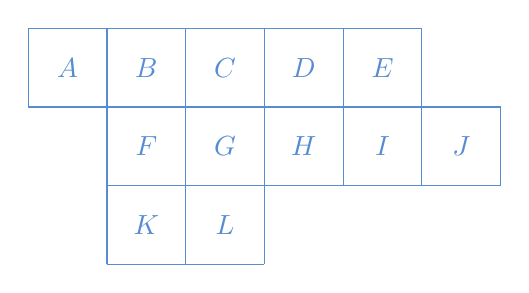
\begin{tikzpicture}[cackithi]
			\draw (0,0) grid (5,1);
			\draw (1,-1) grid (6,0);
			\draw (1,-2) grid (3,-1);
			\draw (0.5,0.5) node{$A$};
			\draw (1.5,0.5) node{$B$};
			\draw (2.5,0.5) node{$C$};
			\draw (3.5,0.5) node{$D$};
			\draw (4.5,0.5) node{$E$};
			\draw (1.5,-0.5) node{$F$};
			\draw (2.5,-0.5) node{$G$};
			\draw (3.5,-0.5) node{$H$};
			\draw (4.5,-0.5) node{$I$};
			\draw (5.5,-0.5) node{$J$};
			\draw (1.5,-1.5) node{$K$};
			\draw (2.5,-1.5) node{$L$};
		\end{tikzpicture}
		\vspace*{-10pt}
	\end{figure}	 
	\textbf{\color{cackithi}Bài} $\pmb{3.}$ Hai hình $ABCDEF$ và $UVWXYZ$ giống hệt nhau về kích thước và hình dáng. Đố bạn biết cạnh nào của hình $UVWXYZ$ có độ dài bằng cạnh $DE$?
	\begin{figure}[H]
		\centering
		\vspace*{-5pt}
		\captionsetup{labelformat= empty, justification=centering}
		\includegraphics[width=1\linewidth]{Bai2}
		\vspace*{-10pt}
	\end{figure}
	\textbf{\color{cackithi}Bài} $\pmb{4.}$ Tháp gỗ sau được xếp bằng các viên gỗ nhỏ hình lập phương, viên này chồng lên viên kia. Có một số viên gỗ không nhìn thấy được.
	\vskip 0.1cm
	Hỏi số viên gỗ không nhìn thấy được nhiều hơn số viên gỗ nhìn thấy được là bao nhiêu viên?
	\begin{figure}[H]
		\centering
		\vspace*{-5pt}
		\captionsetup{labelformat= empty, justification=centering}
		\includegraphics[width=0.7\linewidth]{Bai4}
		\vspace*{-10pt}
	\end{figure}
	\textbf{\color{cackithi}Bài} $\pmb{5.}$ Hình chữ nhật sau được chia thành bốn hình tam giác có diện tích là $2$, $3$, $5$ và $x$ như hình vẽ.
	\begin{figure}[H]
		\centering
		\vspace*{-5pt}
		\captionsetup{labelformat= empty, justification=centering}
		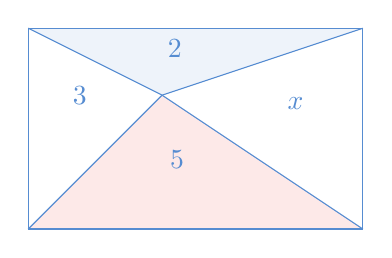
\begin{tikzpicture}[cackithi,scale=0.85]
			\fill[fill=cackithi,fill opacity=0.10000000149011612] (0,3) -- (2,2) -- (5,3) -- cycle;
			\fill[fill=toanhocdoisong,fill opacity=0.10000000149011612] (0,0) -- (2,2) -- (5,0) -- cycle;
			\draw  (0,0)-- (0,3);
			\draw  (0,3)-- (5,3);
			\draw  (5,3)-- (5,0);
			\draw  (5,0)-- (0,0);
			\draw  (0,3)-- (2,2);
			\draw  (2,2)-- (5,3);
			\draw  (5,3)-- (0,3);
			\draw  (0,0)-- (2,2);
			\draw  (2,2)-- (5,0);
			\draw  (5,0)-- (0,0);
			\draw (0.7715297724476833,1.9968077986358754) node {$3$};
			\draw (3.9949386709976675,1.8798965950615238) node {$x$};
			\draw (2.1911658158505265,2.698275020081985) node {$2$};
			\draw (2.2245690168717696,1.0448165695304408) node {$5$};
		\end{tikzpicture}
		\vspace*{-10pt}
	\end{figure}
	Tính giá trị của $x$?
	\vskip 0.1cm 	 
	\textbf{\color{cackithi}Bài} $\pmb{6.}$ Hình sau có bao nhiêu hình tam giác?
	\begin{figure}[H]
		\centering
		\vspace*{-5pt}
		\captionsetup{labelformat= empty, justification=centering}
		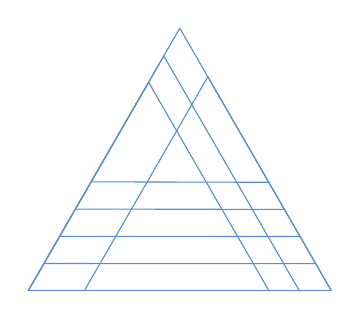
\begin{tikzpicture}[cackithi,scale=0.85]
			\draw  (0,0)-- (4.529389887337568,0);
			\draw  (4.529389887337568,0)-- (2.2646949436687853,3.922566706078671);
			\draw  (2.2646949436687853,3.922566706078671)-- (0,0);
			\draw  (0.8383361744901764,0)-- (4.529389887337568,0);
			\draw  (4.529389887337568,0)-- (2.683863030913873,3.196546282058714);
			\draw  (2.683863030913873,3.196546282058714)-- (0.8383361744901764,0);
			\draw  (0,0)-- (3.59696996366193,0);
			\draw  (3.59696996366193,0)-- (1.7984849818309656,3.115067365180821);
			\draw  (1.7984849818309656,3.115067365180821)-- (0,0);
			\draw  (0,0)-- (4.050858326392901,0);
			\draw  (4.050858326392901,0)-- (2.0254291631964514,3.508146217787968);
			\draw  (2.0254291631964514,3.508146217787968)-- (0,0);
			\draw  (0.9396160733024788,1.6274627785682547)-- (3.5936444563102365,1.6207586294897776);
			\draw  (0.7047120549768591,1.220597083926191)-- (3.827580814067069,1.215568972117333);
			\draw  (0.4698080366512394,0.8137313892841274)-- (4.061517171823902,0.8103793147448888);
			\draw  (0.2349040183256197,0.4068656946420637)-- (4.295453529580735,0.4051896573724444);
		\end{tikzpicture}
		\vspace*{-10pt}
	\end{figure}
	\textbf{\color{cackithi}Bài} $\pmb{7.}$ Các ô vuông của hình sau được điền các số tự nhiên khác $0$ sao cho trên mỗi hàng là các số khác nhau, và số nằm ở ô vuông bên trên bằng tích của hai số được ghi ở hai ô vuông nằm bên dưới nó.
	\begin{figure}[H]
		\centering
		\vspace*{-5pt}
		\captionsetup{labelformat= empty, justification=centering}
		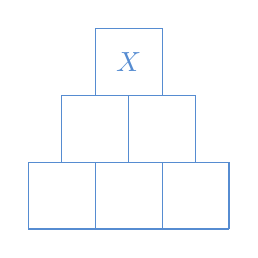
\begin{tikzpicture}[cackithi,scale=0.85]
			\draw (0,0) grid (3,1);
			\draw (1,2) grid (2,3);
			\draw (0.5,1) rectangle (2.5,2);
			\draw (1.5,1) -- (1.5,2);
			\draw (1.5,2.5) node{$X$};
		\end{tikzpicture}
		\vspace*{-10pt}
	\end{figure}
	Hỏi $X$ có giá trị nhỏ nhất bằng bao nhiêu?
	\vskip 0.1cm	
	\textbf{\color{cackithi}Bài} $\pmb{8.}$ Cho $8$ điểm nằm trên một lưới ô vuông như hình vẽ. Hỏi có bao nhiêu tam giác có các đỉnh là $3$ trong số $8$ điểm đã cho.
	\begin{figure}[H]
		\centering
		\vspace*{-5pt}
		\captionsetup{labelformat= empty, justification=centering}
		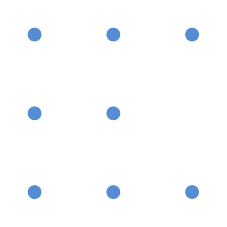
\begin{tikzpicture}
			\fill[cackithi] (0,0) circle (2.5pt);
			\fill[cackithi] (0,1) circle (2.5pt);
			\fill[cackithi] (1,0) circle (2.5pt);
			\fill[cackithi] (1,1) circle (2.5pt);
			\fill[cackithi] (0,2) circle (2.5pt);
			\fill[cackithi] (2,0) circle (2.5pt);
			\fill[cackithi] (1,2) circle (2.5pt);
			\fill[cackithi] (2,2) circle (2.5pt);
		\end{tikzpicture}
		\vspace*{-10pt}
	\end{figure}
	\textbf{\color{cackithi}Bài} $\pmb{9.}$ Trên bảng ghi $9$ số $1,2,3,4,\ldots,9$. Bạn Nam muốn chọn ra một số số có tổng bằng $32$. Hỏi bạn Nam cần chọn ra ít nhất bao nhiêu số?
	\vskip 0.1cm
	\textbf{\color{cackithi}Bài} $\pmb{10.}$ Việt có $3$ chìa khóa để mở $3$ ổ khóa bên ngoài một chiếc hòm đựng báu vật, mỗi chìa chỉ mở được đúng $1$ ổ khóa. Tuy nhiên Việt không nhớ chìa nào ứng với ổ khóa nào. Hỏi Việt phải  tra chìa vào ổ khóa để thử ít nhất mấy lần để chắc chắn xác định được chìa khóa nào là của ổ khóa nào.
	\vskip 0.1cm
	\textbf{\color{cackithi}Bài} $\pmb{11.}$ Điền số thích hợp vào chỗ trống:
	\begin{align*}
		261, 220, 202, 612, 202, 026, \_\_\_
	\end{align*}
	\textbf{\color{cackithi}Bài} $\pmb{12.}$ Biết rằng tổng các chữ số của một số tự nhiên có $3$ chữ số bằng $7$. Liệt kê tất cả các giá trị có thể của tổng các chữ số của số liền trước nó? 
	\vskip 0.1cm
	\textbf{\color{cackithi}Bài} $\pmb{13.}$ Ngày $26$ tháng $12$ năm $2020$ là ngày thứ bảy. Hỏi ngày này sau đúng $60$ năm sau ($26/12/2080$) là thứ mấy?
	\vskip 0.1cm
	\textbf{\color{cackithi}Bài} $\pmb{14.}$ Có bao nhiêu số có $3$ chữ số mà chữ số hàng trăm lớn hơn chữ số hàng đơn vị.
	\vskip 0.1cm
	\textbf{\color{cackithi}Bài} $\pmb{15.}$ Có bao nhiêu cách lát kín một mảnh đất hình chữ nhật kích thước $5(m)\times2(m)$ bằng các tấm bê tông hình chữ nhật kích thước $1(m)\times2(m)$.
	\vskip 0.1cm
	\textbf{\color{cackithi}Bài} $\pmb{16.}$ Điền số thích hợp vào chỗ trống:
	\begin{align*}
		6, 12, 15, 21, 24, 30, \_\_\_
	\end{align*}
	\vskip 0.1cm
	Bài $17$. Có bao nhiêu cách để chia $4$ bạn Đông, Tây, Nam, Bắc thành hai nhóm, mỗi nhóm có $2$ bạn?
	\vskip 0.1cm
	\textbf{\color{cackithi}Bài} $\pmb{18.}$ Có bao nhiêu số điện tử có $3$ chữ số (digital number) mà giá trị của nó không đổi khi ta nhìn trong gương? (số có $3$ chữ số này có chữ số hàng trăm khác $0$).
	\vskip 0.1cm
	\textit{Chữ số điện tử:} 
	\begin{figure}[H]
		\centering
		\vspace*{-10pt}
		\captionsetup{labelformat= empty, justification=centering}
		\includegraphics[width=1\linewidth]{Bai18}
		\vspace*{-15pt}
	\end{figure}
	\textbf{\color{cackithi}Bài} $\pmb{19.}$ Trên bảng ta vẽ $5$ đường tròn (không có hai đường tròn nào trùng nhau), hỏi $5$ đường tròn này cắt nhau tại nhiều nhất bao nhiêu điểm? 
	\vskip 0.1cm
	\textbf{\color{cackithi}Bài} $\pmb{20.}$ Có bao nhiêu số có ba chữ số chia hết cho $3$ mà không chứa chữ số $3$?
	\vskip 0.1cm
	\textbf{\color{cackithi}Lời giải, đáp án}
	\vskip 0.1cm
	\textbf{\color{cackithi}Bài} $\pmb{1.}$ Đáp số: $32+40+52+68+88+112=392$ $(mm)$.
	\vskip 0.1cm
	\textbf{\color{cackithi}Bài} $\pmb{2.}$ Đáp số: $G$.
	\vskip 0.1cm
	\textbf{\color{cackithi}Bài} $\pmb{3.}$ Đáp số: $UV$.	 
	\vskip 0.1cm
	\textbf{\color{cackithi}Bài} $\pmb{4.}$
	\textit{Lời giải} $1$.
	Tổng số viên: $1\times5+2\times4+3\times3+4\times2+5 = 35$.
	\vskip 0.1cm
	Số viên nhìn thấy: $1+2+3+4+5 = 15$.
	\vskip 0.1cm
	Số viên không nhìn thấy: $35 - 15 = 20$.
	\vskip 0.1cm
	Đáp số: $20 - 15 = 5$.
	\vskip 0.1cm
	\textit{Lời giải} $2$.
	Số viên nhìn thấy: $1+2+3+4+5 = 15$.
	\vskip 0.1cm
	Số viên không nhìn thấy: $4 + 3\times2 + 2\times3 + 1\times4 = 20$.
	\vskip 0.1cm
	Đáp số: $20 - 15 = 5$.
	\vskip 0.1cm
	\textbf{\color{cackithi}Bài} $\pmb{5.}$ \textit{Lời giải}.
	Hai tam giác Xanh, Đỏ có đáy bằng nhau bằng chiều dài hình chữ nhật, tổng chiều cao bằng chiều rộng hình chữ nhật $\Rightarrow$ Tổng diện tích bằng một nữa hình chữ nhật. Vậy ta có:
	\begin{align*}
			2 + 5 = 3 + X \Rightarrow X = 4.
		\end{align*}
	Đáp số: $4$.
	\vskip 0.1cm
	\textbf{\color{cackithi}Bài} $\pmb{6.}$ \textit{Lời giải}.
	Như trên hình vẽ, mỗi tam giác có đáy, cạnh bên trái và cạnh bên phải.
	\vskip 0.1cm
	Chọn đáy: $5$ (cách).
	\vskip 0.1cm
	Chọn cạnh bên phải: $3$ (cách). 
	\vskip 0.1cm
	Chọn cạnh bên trái: $2$ (cách).
	\vskip 0.1cm
	Theo quy tắc nhân, số tam giác là: $5\times3\times2 = 30$.
	\vskip 0.1cm
	Đáp số: $30$.
	\vskip 0.1cm
	\textbf{\color{cackithi}Bài} $\pmb{7.}$ \textit{Lời giải}.
	\begin{figure}[H]
		\centering
		\vspace*{-5pt}
		\captionsetup{labelformat= empty, justification=centering}
		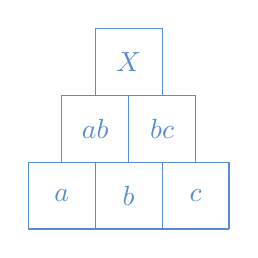
\begin{tikzpicture}[cackithi, scale=0.85]
				\draw (0,0) grid (3,1);
		\draw (1,2) grid (2,3);
		\draw (0.5,1) rectangle (2.5,2);
		\draw (1.5,1) -- (1.5,2);
		\draw (1.5,2.5) node{$X$};
		\draw(0.5,0.5) node{$a$};
		\draw(1.5,0.5) node{$b$};
		\draw(2.5,0.5) node{$c$};
		\draw(1,1.5) node{$ab$};
		\draw(2,1.5) node{$bc$};
		\end{tikzpicture}
		\vspace*{-10pt}
	\end{figure}
	Gọi $3$ số hàng cuối là $a,b,c$ ($a\ne b\ne c > 0$).
	\vskip 0.1cm
	Hàng $2$ có $2$ số là: $ab$ và $bc$.
	\vskip 0.1cm
	Vậy $X = ab\times bc = ab^2c$ bé nhất khi $b=1$, $a=2$, $c=3$ hoặc $b=1$, $a=3$, $c=2$.
	\vskip 0.1cm
	Vậy giá trị nhỏ nhất của $X$ là: $2\times 1^2\times3 = 6$.
	\vskip 0.1cm
	Đáp số: $6$
	\vskip 0.1cm
	\textbf{\color{cackithi}Bài} $\pmb{8.}$ \textit{Lời giải}.
	Số cách chọn $3$ điểm: 
	\begin{align*}
			C_8^3 = \frac{8\times 7 \times 6}{3!} = 56.
		\end{align*}
	Số tam giác suy biến (tam giác có $3$ điểm thẳng hàng): $6$.
	\vskip 0.1cm
	Số tam giác là: $56 - 6 = 50$.
	\vskip 0.1cm
	\textbf{\color{cackithi}Bài} $\pmb{9.}$ \textit{Lời giải}. 
	Để chọn ít nhất Nam cần rút những số lớn nhất có thể.
	\vskip 0.1cm
	$32 = 9 + 8 + 7 + 6 + 2$. Vậy Nam cần chọn $5$ số $(9,8,7,6,2)$.
	\vskip 0.1cm
	Đáp số: $5$.
	\vskip 0.1cm
	\textbf{\color{cackithi}Bài} $\pmb{10.}$ \textit{Lời giải}.
	Thử chìa đầu tiên: $2$ lần thử thì xác định được sẽ mở ổ nào (Nếu $2$ lần thử không được thì chìa sẽ mở được ổ còn lại).
	\vskip 0.1cm
	Thử chìa $2$: $1$ lần sẽ xác định được mở ổ nào.
	\vskip 0.1cm
	Chìa còn lại sẽ mở được ổ còn lại. Vậy số lần thử ít nhất là: $2+1=3$.
	\vskip 0.1cm
	Đáp số: $3$.
	\vskip 0.1cm
	\textbf{\color{cackithi}Bài} $\pmb{11.}$ \textit{Lời giải}.
	$2612202026122020\ldots$ nó chính là dãy $26/12/2020$ lặp đi lặp lại.
	\vskip 0.1cm
	Vậy số tiếp theo là $122$.
	\vskip 0.1cm
	Đáp số: $122$.
	\vskip 0.1cm
	\textbf{\color{cackithi}Bài} $\pmb{12.}$. \textit{Lời giải} $1$.
	Nếu số đó là $700$. Số liền trước là $699$ có tổng các chữ số bằng $6+9+9=24$.
	\vskip 0.1cm
	Nếu số đó là: $\overline{ab0}$ ($b\ne0$), số liền trước là: $\overline{(a(b-1)9)}$ có tổng các chữ số 
	bằng
	\begin{align*}
			a+b-1+9=a+b+8=7+8=15.
		\end{align*}
	Nếu số đó là $\overline{abc}$ ($c\ne0$), số liền trước là: $\overline{ab(c-1)}$ có tổng các chữ số bằng
	\begin{align*}
			a+b+c-1=7-1=6.
		\end{align*}
	Vậy các giá trị có thể của tổng các chữ số liền trước là: $\{6,15,24\}$.
	\vskip 0.1cm 
	\textit{Lời giải} $2$.
	Số có $3$ chữ số có tổng các chữ số bằng $7$ chia $9$ dư $7$. Vậy số liền trước là số có $3$ chữ số chia $9$ dư $6$. Vậy tổng các chữ số của nó có thể nhận các giá trị $\{6,15,24\}$ (do $9\times 3 = 27 < 33$). Thử với $3$ số $115$, $160$, $700$ có các số liền trước là $114$, $159$, $699$ có tổng các chữ số tương ứng là $6$, $15$, $24$.
	\vskip 0.1cm
	\textit{Lời giải} $3$. Liệt kê các số có $3$ chữ số thỏa mãn là $106$, $115$, $124$, $133$, $142$, $151$, $160$, $205$, $214$, $223$, $232$, $241$, $250$, $304$, $313$, $322$, $331$, $340$, $403$, $412$, $421$, $430$, $502$, $511$, $520$, $601$, $610$, $700$.
	\vskip 0.1cm
	Số liền trước: $105\ldots$, $159$, $249$, $339$, $429$, $519$, $609$, $699$ có tổng các chữ số là: $6$, $15$, $24$.
	\vskip 0.1cm
	Đáp số: $6$, $15$, $24$.
	\vskip 0.1cm
	\textbf{\color{cackithi}Bài} $\pmb{13.}$ \textit{Lời giải}.
	Năm thường có $365$ ngày chia $7$ dư $1$ $\Rightarrow$ $60\times 365$ chia $7$ dư $4$.
	\vskip 0.1cm
	$60$ năm có $60:4=15$ năm nhuận, thêm $15$ ngày, chia $7$ dư $1$.
	\vskip 0.1cm
	Vậy số ngày trong $60$ năm chia $7$ dư $5$, vậy sau $5$ ngày từ thứ $7$ là thứ $5$.
	\vskip 0.1cm
	Đáp số: Thứ $5$.
	\vskip 0.1cm
	\textbf{\color{cackithi}Bài} $\pmb{14.}$ \textit{Lời giải}.
	Gọi số đó là $\overline{abc}$.
	\vskip 0.1cm
	+ $b$ có $10$ cách chọn.
	\vskip 0.1cm
	+ $\overline{ac}$ có số cách chọn là: $1+2+3+\ldots+9 = 45$ (Hoặc mỗi cặp $2$ chữ số có đúng $1$ số $\overline{ac}$ thỏa mãn $a>c$ nên số cách chọn $\overline{ac}$ là: $C^2_{10} = 45$).
	\vskip 0.1cm
	Vậy số số có $3$ chữ số thỏa mãn là: $10\times45=450$.
	\vskip 0.1cm
	Đáp số: $450$ .
	\vskip 0.1cm
	\textbf{\color{cackithi}Bài} $\pmb{15.}$ \textit{Hướng dẫn giải}.
	Số cách lát hình chữ nhật $k(m) \times 2(m)$ bằng các viên gạch $1(m)\times2(m)$ chính là dãy Fibonacci $1,2,3,5,8,\ldots$. Vậy số cách lát là: $F5 = 8$.
	\vskip 0.1cm
	Đáp số: $8$.
	\vskip 0.1cm
	\textbf{\color{cackithi}Bài} $\pmb{16.}$ Đáp số: $33$.
	\vskip 0.1cm 
	\textbf{\color{cackithi}Bài} $\pmb{17.}$ \textit{Lời giải}. Đông có thể ghép cặp với Tây, Nam hoặc Bắc. Vậy có $3$ cách chia nhóm.
	\vskip 0.1cm
	Đáp số: $3$.
	\vskip 0.1cm
	\textbf{\color{cackithi}Bài} $\pmb{18.}$ \textit{Lời giải}.
	Gọi số có $3$ chữ số là: $\overline{abc}$.
	\vskip 0.1cm
	+ Số cách chọn $b$ là $3$ $(0,1,8)$.
	\vskip 0.1cm
	+ Số cách chọn $\overline{ac}$ là: $4$ $(11, 88,25, 52)$.
	\vskip 0.1cm
	Đáp số: $3\times 4=12$.
	\vskip 0.1cm
	\textbf{\color{cackithi}Bài} $\pmb{19.}$ \textit{Lời giải}. Số điểm cắt nhiều nhất xảy ra khi hai đường tròn bất kỳ đều cắt nhau tại $2$ điểm và không có $3$ đường tròn nào cắt nhau tại $1$ điểm. Khi đó mỗi đường tròn cắt $4$ đường tròn kia tại $4\times 2=8$ điểm $\Rightarrow$ Số điểm cắt sẽ là: $8\times 5 = 40$, tuy nhiên mỗi điểm sẽ được tính $2$ lần (vì đường tròn $A$ cắt $B$ tại $2$ điểm chính là $2$ điểm của đường tròn $B$ cắt $A$). Vậy số điểm cắt nhiều nhất của $5$ đường tròn là: $40:2 = 20$.
	\vskip 0.1cm
	Đáp số: $20$ (điểm).
	\vskip 0.1cm
	\textbf{\color{cackithi}Bài} $\pmb{20.}$ \textit{Lời giải}. 
	Gọi số đó là $\overline{abc}$.
	\vskip 0.1cm
	Nếu $\overline{ab}$ chia $3$ dư $0$: $c\in \{0,6,9\}$ -- có $3$ cách chọn $c$.
	\vskip 0.1cm  
	Nếu $\overline{ab}$ chia $3$ dư $1$: $c\in \{2,5,8\}$ -- có $3$ cách chọn $c$.
	\vskip 0.1cm  
	Nếu $\overline{ab}$ chia $3$ dư $2$: $c\in \{1,4,7\}$ -- có $3$ cách chọn $c$.
	\vskip 0.1cm  
	Vậy với mỗi số $\overline{ab}$ đều có $3$ cách chọn $c$. Số các số có $2$ chữ số đều khác $3$ là: $8\times9=72$.
	\vskip 0.1cm
	Số số có $3$ chữ số thỏa mãn là: $72\times 3=216$.
	\vskip 0.1cm
	Đáp số: $216$. 
\end{multicols}
\newpage
\begingroup
\AddToShipoutPicture*{\put(150,695){\includegraphics[scale=1]{../tieude1.pdf}}}
\centering
\endgroup
\vspace*{10pt}
\begin{multicols}{2}
	Trong phần đầu chuyên mục, chúng tôi sẽ trình bày \textit{Lời giải} của các bài toán trong kỳ thi  Olympic Toán học Trẻ của Canada năm học $2022$  đăng trong số báo $11/2022$. 
	\begin{figure}[H]
		\centering
		\vspace*{-5pt}
		\captionsetup{labelformat= empty, justification=centering}
		\includegraphics[width=1\linewidth]{gocolympic}
		\vspace*{-10pt}
	\end{figure}
	{\bf\color{cackithi} OC$\pmb{25.}$} Cho $ABC$ là tam giác nhọn nội tiếp đường tròn $\Gamma.$ Đường thẳng qua $A$ vuông góc với $BC$ cắt $\Gamma$ tại $D,$ và đường thẳng qua $B$ vuông góc với $AC$ cắt $\Gamma$ tại $E.$ Chứng minh rằng nếu $AB = DE$, thì $\angle ACB = 60^{\circ}.$
	\vskip 0.1cm
	\textit{\textit{Lời giải}.} 
	\begin{figure}[H]
		\vspace*{-5pt}
		\centering
		\captionsetup{labelformat= empty, justification=centering}
		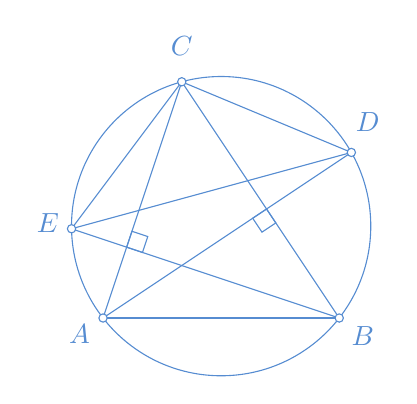
\begin{tikzpicture}[cackithi]
			\draw (0.9004185552987112,2.2669457035324743) -- (1.0180882363816217,2.0904411819081083) -- (1.1945927580059874,2.208110862991019) -- (1.0769230769230769,2.3846153846153846) -- cycle; 
			\draw (-0.4987538820250189,1.8329179606750063) -- (-0.4316718427000252,2.0341640786499875) -- (-0.6329179606750064,2.101246117974981) -- (-0.7,1.9) -- cycle; 
			\draw  (0.5,2.1666666666666665) circle (1.9002923751652299cm);
			\draw  (-1.,1.)-- (2.,1.);
			\draw  (2.,1.)-- (0.,4.);
			\draw  (0.,4.)-- (-1.,1.);
			\draw  (-1.,1.)-- (2.1538461538461533,3.102564102564102);
			\draw  (2.,1.)-- (-1.4,2.1333333333333333);
			\draw  (-1.4,2.1333333333333333)-- (2.1538461538461533,3.102564102564102);
			\draw  (2.1538461538461533,3.102564102564102)-- (0.,4.);
			\draw  (0.,4.)-- (-1.4,2.1333333333333333);
				\draw [fill=white] (-1.,1.) circle (1.5pt);
				\draw (-1.3,0.79) node {$A$};
				\draw [fill=white] (2.,1.) circle (1.5pt);
				\draw (2.3,0.77) node {$B$};
				\draw [fill=white] (0.,4.) circle (1.5pt);
				\draw (0.,4.45) node {$C$};
				\draw [fill=white] (2.1538461538461533,3.102564102564102) circle (1.5pt);
				\draw (2.36,3.49) node {$D$};
				\draw [fill=white] (-1.4,2.1333333333333333) circle (1.5pt);
				\draw (-1.7,2.21) node {$E$};
		\end{tikzpicture}
		\vspace*{-10pt}
	\end{figure}
	Do $ABC$ là tam giác nhọn nên các điểm $D$ và $E$ lần lượt nằm ở bên trong cung nhỏ $BC$ và $AC$ như trong hình vẽ. Như vậy $\angle ECD$ lớn hơn  $\angle ACB$. Từ giả thiết $AB=DE,$ ta có $\angle ECD= 180^\circ - \angle ACB$.  \hfill ($1$)
	\vskip 0.1cm
	Mặt khác ta có
	\begin{align*}
		\angle ECD =\,&\angle ECA + \angle ACB + \angle BCD \\
		= \,&\angle EBA + \angle ACB + \angle BAD \\
		= \,&90^\circ \!\!-\!\! \angle BAC \!\!+\!\! \angle ACB \!\!+\!\! 90^\circ \!\!-\!\! \angle ABC \\
		= \,&(180^\circ \!-\! \angle BAC \!-\! \angle ABC) \!+\! \angle ACB  \\
		= \,&2\angle ACB  \tag{$2$}
	\end{align*}
	Từ ($1$) và ($2$) ta nhận được điều cần chứng minh.
	\vskip 0.1cm
	{\bf\color{cackithi} OC$\pmb{26.}$} Giả sử bạn có vô hạn các hình chữ $T$ (bao gồm bốn hình vuông cạnh
	$1$) như trong hình vẽ, và một bảng ô vuông cỡ $n \times n.$ Bạn được phép đặt một số hình trên bảng (có thể xoay chúng), miễn là không có hai hình nào chồng lên nhau và không có hình nào vượt ra khỏi bảng.
	\vskip 0.1cm
	Với những giá trị nào của $n$ thì bạn có thể phủ toàn bộ bảng?
	\begin{figure}[H]
		\vspace*{-5pt}
		\centering
		\captionsetup{labelformat= empty, justification=centering}
		\begin{tikzpicture}[cackithi,scale=0.88]
			\draw (0,0) grid (3,1);
			\draw (1,-1) grid (2,0);
		\end{tikzpicture}
		\vspace*{-10pt}
	\end{figure}
	\textit{\textit{Lời giải}.} Trước tiên ta nhận thấy mỗi hình chữ $T$ gồm $4$ ô, do đó nếu phủ kín được bảng thì diện tích của bảng phải chia hết cho $4$, tức là $n$ chẵn.
	\vskip 0.1cm
	Với $n$ chia hết cho $4$ ta có thể chia bảng thành các bảng con cỡ $4\times 4$ và phủ kín mỗi bảng con bằng $4$ hình chữ $T$ như sau:
	\begin{figure}[H]
		\vspace*{-5pt}
		\centering
		\captionsetup{labelformat= empty, justification=centering}
		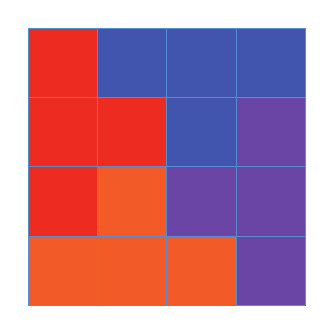
\begin{tikzpicture}[cackithi,scale=0.88]
			\filldraw[duongvaotoanhoc] (0,0) rectangle (3,1);
			\filldraw[gocco] (3,0) rectangle (4,3);
			\filldraw[timhieukhoahoc] (4,3) rectangle (1,4);
			\filldraw[toanhocdoisong] (0,1) rectangle (1,4);
			\filldraw[duongvaotoanhoc] (1,1) rectangle (2,2);
			\filldraw[gocco] (2,1) rectangle (3,2);
			\filldraw[timhieukhoahoc] (2,2) rectangle (3,3);
			\filldraw[toanhocdoisong] (1,2) rectangle (2,3);
			\draw (0,0) grid (4,4);
		\end{tikzpicture}
		\vspace*{-10pt}
	\end{figure}
	Với $n=4k+2,$ ta tô màu đen, trắng các ô trong bảng như bàn cờ vua. Để lát kín bảng cần tất cả $\dfrac{n^2}{4}=(2k+1)^2$ hình chữ $T$. Như vậy có một số lẻ hình chữ $T$ và mỗi hình phủ $1$ hoặc $3$ ô đen, tức là tổng số ô đen phải là lẻ. Nhưng thực tế có  $\dfrac{n^2}{2}=2(2k+1)^2$ ô đen. Do đó trường hợp này không thể phủ kín bảng như yêu cầu. 
	\begin{figure}[H]
		\vspace*{-5pt}
		\centering
		\captionsetup{labelformat= empty, justification=centering}
		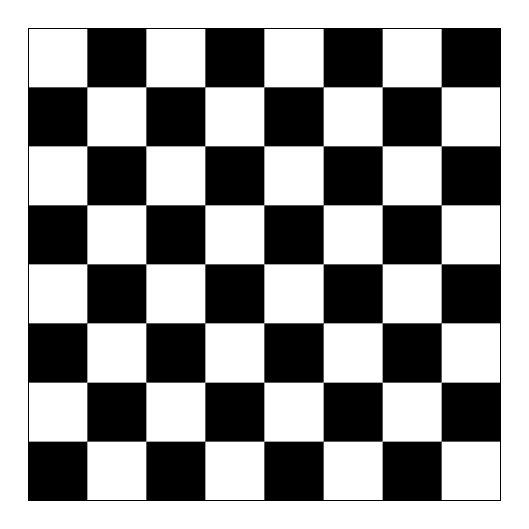
\begin{tikzpicture}[scale=0.75]
			\draw (0,0) rectangle (8,8);
			\foreach \y in {0,2,...,6}{
				\foreach \x in {0,2,...,6}{
					\fill (\x,\y) rectangle (1+\x,1+\y) rectangle (2+\x,2+\y);}}
		\end{tikzpicture}
		\vspace*{-5pt}
	\end{figure}
	Tóm lại ta phủ kín được bảng bằng các hình chữ $T$ khi và chỉ khi $n$ chia hết cho $4$.
	\vskip 0.1cm
	{\bf\color{cackithi} OC$\pmb{27.}$} Giả sử rằng các số thực $a$ và $b$ thỏa mãn
	\begin{align*}
		ab+ \sqrt{ab+1} +\sqrt{a^2+b}\ \sqrt{b^2+a}=0.
	\end{align*}
	Tìm giá trị của biểu thức
	\begin{align*}
		S=a\sqrt{b^2+a} + b\sqrt{a^2+b}.
	\end{align*}
	\textit{\textit{Lời giải}.} Từ đẳng thức trong bài, chuyển vế và bình phương hai vế ta có
	\begin{align*}
		& \ ab+ \sqrt{a^2+b} \sqrt{b^2+a} = -\sqrt{ab+1} \\
		\Rightarrow\  &	a^2b^2 + 2ab\sqrt{a^2+b} \sqrt{b^2+a} \\
		&+ (a^2+b)(b^2+a) = ab+1\\
		\Leftrightarrow\  &	(a^2b^2+a^3) + 2ab\sqrt{a^2+b} \sqrt{b^2+a} \\
		&+ (b^3+a^2b^2) = 1\\
		\Leftrightarrow\ 	& (a\sqrt{b^2+a} + b\sqrt{a^2+b})^2 = 1.
	\end{align*}
	Ta nhận được $S=\pm 1.$ Ta sẽ chứng minh $S$ luôn dương. Thực vậy, từ giả thiết ta có
	\begin{align*}
		ab= -\sqrt{ab+1} -\sqrt{a^2+b} \sqrt{b^2+a} <0.
	\end{align*}
	Không mất tổng quát, ta có thể giả sử \linebreak $a>0>b.$ Khi đó, do $a>\sqrt{a^2+b},$ ta có
	\begin{align*}
		S= a( \sqrt{b^2+a} +b)- b(a- \sqrt{a^2+b})>0.
	\end{align*} 
	Do đó  $S=1$.
	\vskip 0.1cm
	Trong phần cuối của chuyên mục kỳ này, chúng tôi sẽ giới thiệu với bạn đọc ba bài toán trong kỳ thi Olympic Toán học trẻ khối Pháp ngữ năm $2022$. Các bài toán này phù hợp với trình độ học sinh năm cuối cấp Trung học cơ sở.
	\vskip 0.1cm
	{\bf\color{cackithi} OC$\pmb{34.}$} Tìm tất cả các số nguyên dương $n$ sao cho $ \lfloor \sqrt{n}\rfloor $ là ước của $n.$ 
	\vskip 0.1cm
	\textit{Chú ý}: $ \lfloor x \rfloor $ ký hiệu phần nguyên của một số thực $x,$ được định nghĩa là số nguyên lớn nhất nhỏ hơn hoặc bằng $x.$ Ví dụ: $ \lfloor 1.4 \rfloor =1$, $ \lfloor 2 \rfloor=2,$ và  $ \lfloor 2.9 \rfloor= 2.$  
	\vskip 0.1cm
	{\bf\color{cackithi} OC$\pmb{35.}$} Cho một bảng ô vuông cỡ $n \times n$ với $n\ge 1$. Aya muốn tô màu  $k$ ô của bảng  sao cho chỉ có duy nhất một cách để đặt  $n$ đồng xu trên các ô vuông được tô màu sao cho không có hai đồng xu nào nằm trên cùng một hàng hoặc cột. Hỏi giá trị tối đa có thể của $k$  là bao nhiêu?
	\vskip 0.1cm
	{\bf\color{cackithi} OC$\pmb{36.}$} Cho tam giác $ABC$ và $D$ là giao điểm của đường phân giác của góc $\angle BAC$ và đường trung trực của cạnh $AC$. Đường thẳng  đi qua $B$ và song song với $AC$, cắt đường thẳng $AD$ tại $X$. Đường thẳng đi qua $B$ và song song với $CX$, cắt đường thẳng $AC$ tại $Y$. Đường tròn ngoại tiếp tam giác $ABY$ cắt đường thẳng $BX$ tại $E.$ Chứng minh rằng ba điểm $C$ , $D$ và $E$ thẳng hàng.
\end{multicols}
%	\newpage
%	
%	\setcounter{figure}{0}
%	\thispagestyle{lichsutoanhocnone}
\pagestyle{lichsutoanhoc}
\graphicspath{{../lichsutoanhoc/pic/}}
\everymath{\color{lichsutoanhoc}}
%\blfootnote{$^1$\color{lichsutoanhoc}Hà Nội.}
\begingroup
\AddToShipoutPicture*{\put(0,616){\includegraphics[width=19.3cm]{../bannerlichsu}}}
\AddToShipoutPicture*{\put(62,517){\includegraphics[scale=1]{../tieude.pdf}}}
\centering
\endgroup

\vspace*{185pt}

\begin{multicols}{2}
	Một số vô tỷ rất quen thuộc và có nhiều ý nghĩa thực tế là tỷ số giữa chu vi đường tròn và đường kính của nó, lần đầu tiên được nhà toán học Anh William Jones ($1675-1749$) ký hiệu bằng chữ $\pi$ vào năm $1706$  trong cuốn sách \textit{Synopsis Palmariorum Matheseos} (\textit{Nhập môn Toán học mới}). Chữ $\pi$ là chữ cái đầu tiên trong chữ Hy Lạp \textit{περιφέρεια} (\textit{periphery--viền ngoài, chu vi}). Năm $1748$, trong cuốn sách rất phổ biến, \textit{Introductio in analysin infinitorum} (\textit{Nhập môn Giải tích vô hạn}), Euler viết: ``\textit{để ngắn gọn, ta sẽ ký hiệu $\pi$ bằng một nửa chu vi của đường tròn bán kính bằng $1$}". Từ đó $\pi$ được phổ biến ở châu Âu và ngày nay đã trở thành ký hiệu toán học quen thuộc với tất cả mọi người.
	\vskip 0.1cm
	\textbf{\color{lichsutoanhoc}Số Pi trước toán học Hy Lạp}
	\vskip 0.1cm
	Người Babylon (khoảng $1800-1600$ trước Công nguyên) tính chu vi một đường tròn bằng ba lần đường kính của nó. Hơn nữa, họ còn chính xác hơn khi chọn diện tích hình tròn theo công thức $S = \dfrac{2}{{25}}{L^2},$  trong đó $L$  là chu vi hình tròn. Như vậy, so với công thức chính xác $S = \pi {R^2} = \dfrac{1}{{4\pi }}{\left( {2\pi R} \right)^2}$  thì số  khá chính xác với $\pi  \approx 3{,}1416$.
	\vskip 0.1cm
	Bài toán $48$ trong bản giấy cói Ahmes (Ahmes Rhind Papyrus, $1850$ trước Công nguyên) phát biểu như sau. \textit{Đường tròn có đường kính $9$ khet} (đơn vị độ dài). \textit{Diện tích của nó là bao nhiêu?}
	\vskip 0.1cm
	\textit{Giải:} Bỏ đi $\dfrac{1}{9}$ trong đường kính, cụ thể là $1$, còn $8$. Nhân $8$ với $8$, diện tích của nó là $64$.
	\vskip 0.1cm 
	Bài toán này cho thấy, người Ai Cập cổ đại đã tính diện tích  $S$ của hình tròn có đường kính $d$ bằng diện tích hình vuông có cạnh bằng $\dfrac{8}{9}d$: 
	\setlength{\abovedisplayskip}{5pt}
	\setlength{\belowdisplayskip}{5pt}
	\begin{align*}
		S = {\left( {d - \dfrac{1}{9}d} \right)^2} = {\left( {\dfrac{8}{9}d} \right)^2} = \dfrac{{64}}{{81}}{d^2}.
	\end{align*}
	Từ đây ta có  $S = \dfrac{{64}}{{81}}{d^2} \approx  \pi \dfrac{{{d^2}}}{4}$. Suy ra
	\begin{align*}
		\pi  \approx  \dfrac{{64 \times 4}}{{81}} = \dfrac{{256}}{{81}} \approx 3{,}16049.
	\end{align*}
	Sai số của số này so với  $\pi  \approx 3{,}14156$ là gần $2\%$ và có phân số xấp xỉ là $3\dfrac{1}{7} = \dfrac{{22}}{7} \approx 3{,}14286$.
	\vskip 0.1cm 
	Giả sử cắt ở bốn góc của hình vuông cạnh $9$ \textit{khet} (đơn vị dài) bốn tam giác vuông cân có cạnh bằng $3$ \textit{khet}. Khi ấy diện tích bát giác còn lại gần bằng diện tích hình tròn (hình tròn có phần nằm trong, cũng có phần nằm ngoài bát giác, Hình $1$). Ta có ${S_{{\text{bát giác}}}} = {9^2} - 4.\dfrac{{{3^2}}}{2} = 63.$   
	Giá trị này gần với giá trị  $S = {\left( {\dfrac{8}{9}d} \right)^2} = 64$ khi cho $d = 9$, là cơ sở để giải thích công thức tính diện tích hình tròn $S = \dfrac{{64}}{{81}}{d^2}$  của người Babylon.	 
	\begin{figure}[H]
		\vspace*{-5pt}
		\centering
		\captionsetup{labelformat= empty, justification=centering}
		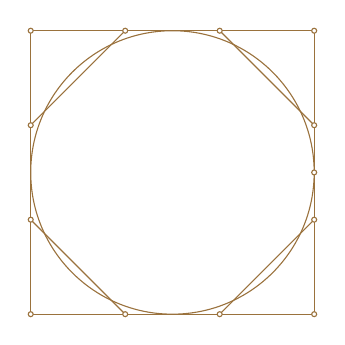
\begin{tikzpicture}[lichsutoanhoc, scale=0.6]
			\draw  (0.,0.) circle (3.cm);
			\draw  (-3.,-3.)-- (3.,-3.);
			\draw  (3.,-3.)-- (3.,3.);
			\draw  (3.,3.)-- (-3.,3.);
			\draw  (-3.,3.)-- (-3.,-3.);
			\draw  (1.,3.)-- (3.,1.);
			\draw  (3.,-1.)-- (1.,-3.);
			\draw  (-1.,-3.)-- (-3.,-1.);
			\draw  (-3.,1.)-- (-1.,3.);
				\draw [fill=white] (3.,0.) circle (1.5pt);
				\draw [fill=white] (-3.,-3.) circle (1.5pt);
				\draw [fill=white] (3.,-3.) circle (1.5pt);
				\draw [fill=white] (3.,3.) circle (1.5pt);
				\draw [fill=white] (-3.,3.) circle (1.5pt);
				\draw [fill=white] (1.,3.) circle (1.5pt);
				\draw [fill=white] (3.,1.) circle (1.5pt);
				\draw [fill=white] (3.,-1.) circle (1.5pt);
				\draw [fill=white] (1.,-3.) circle (1.5pt);
				\draw [fill=white] (-1.,-3.) circle (1.5pt);
				\draw [fill=white] (-3.,-1.) circle (1.5pt);
				\draw [fill=white] (-3.,1.) circle (1.5pt);
				\draw [fill=white] (-1.,3.) circle (1.5pt);
		\end{tikzpicture}
		\caption{\small\textit{\color{lichsutoanhoc}Hình $1$.}}
		\vspace*{-10pt}
	\end{figure}
	Trong bài toán khắc trên bảng đồng của người Babylon, số $\pi$  được chọn bằng $\dfrac{{25}}{8} = 3{,}125$.
	\vskip 0.1cm   
	Khi đo đạc Đại kim tự tháp Giza ($2500$ trước Công nguyên), các nhà khảo cổ học đã nhận thấy người Ai Cập chọn số $\pi$  bằng $\dfrac{{22}}{7} \approx 3{,}14$.
	\vskip 0.1cm   
	Người  Do Thái cũng lấy $\pi = 3$.  Điều này được thấy trong kinh Cựu Ước, khi nói về bồn tắm tròn trong lâu đài của nhà vua Salomon. 
	\vskip 0.1cm
	\textbf{\color{lichsutoanhoc}Số Pi trong toán học Hy Lạp}
	\vskip 0.1cm
	Thuật toán đầu tiên tính gần đúng số $\pi$  được nhà toán học Hy Lạp Archimedes (khoảng $287-212$ trước Công nguyên) trình bày trong cuốn sách  \textit{Measurement of the Circle} (\textit{Đo hình tròn}). Ông  đã tính được 
	\begin{align*}
		3\dfrac{{10}}{{71}} < \pi  < 3\dfrac{{10}}{{70}} \tag{$1$}
	\end{align*}
	bằng cách xét các đa giác đều $96$ cạnh nội tiếp và ngoại tiếp đường tròn như sau. 
	\vskip 0.1cm
	Giả sử $p_n$  và  $P_n$ là chu vi các đa giác đều $n$  cạnh nội tiếp và ngoại tiếp đường tròn chu vi $C$.  Khi ấy ta có 
	\begin{align*}
		{p_6} &< {p_{12}} < {p_{24}} < {p_{48}} < {\rm{ }}{p_{96}} < ... < {p_n} \\
		&< ... < C < ... < {P_n} < ... < {P_{96}} < {P_{48}} \\
		&< {P_{24}} < {P_{12}} < {P_6}.
	\end{align*}
	Dãy số $\{p_n\}$  là dãy số tăng, bị chặn trên bởi $C$  và $\{P_n\}$  là dãy số giảm bị chặn dưới bởi $C$.  Do đó chúng có giới hạn và có thể chứng minh giới hạn chung của chúng là  $C$.
	\vskip 0.1cm
	Giả sử  $Z$ là tâm hình tròn, và $AB = 2t$  và $CD = 2s$   tương ứng là độ dài một cạnh của các đa giác đều $n$  cạnh ngoại tiếp và nội tiếp hình tròn. Gọi $M$  là điểm giữa của $AB$, $N$ là điểm giữa của  $CD$ và $O$  là giao điểm của tiếp tuyến tại điểm  $C$ với $MA$  (Hình $2$). Tương ứng $OM = OC = t'$  là nửa cạnh của đa giác đều $2n$  cạnh ngoại tiếp và $MC = MD = 2s'$ là cạnh của đa giác đều $2n$ cạnh nội tiếp đường tròn.     
	\begin{figure}[H]
		\vspace*{-5pt}
		\centering
		\captionsetup{labelformat= empty, justification=centering}
		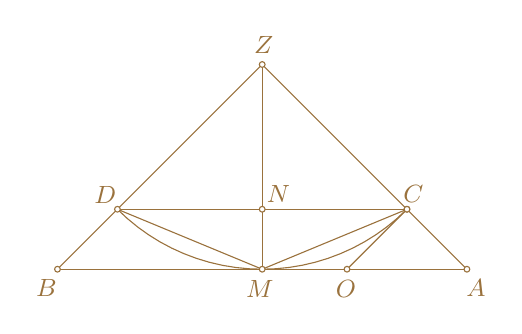
\begin{tikzpicture}[lichsutoanhoc,scale=1.3,node font= \small]
			\draw  (-1.414213562373095,-1.4142135623730954)-- (1.414213562373095,-1.414213562373095);
			\draw [shift={(0.,0.)},]  plot[domain=3.9269908169872414:5.497787143782138,variable=\t]({1.*2.*cos(\t r)+0.*2.*sin(\t r)},{0.*2.*cos(\t r)+1.*2.*sin(\t r)});
			\draw  (0.,0.)-- (-2.,-2.);
			\draw  (-2.,-2.)-- (2.,-2.);
			\draw  (2.,-2.)-- (0.,0.);
			\draw  (-1.414213562373095,-1.4142135623730954)-- (4.214684851089403E-8,-2.);
			\draw  (4.214684851089403E-8,-2.)-- (1.4142135623730958,-1.414213562373095);
			\draw  (0.8284271247461907,-2.)-- (1.4142135623730958,-1.414213562373095);
			\draw  (0.,0.)-- (4.214684851089403E-8,-2.);
				\draw [fill=white] (-2.,-2.) circle (0.8pt);
				\draw (-2.1070556519764487,-2.185112519201409) node {$B$};
				\draw [fill=white] (2.,-2.) circle (0.8pt);
				\draw (2.0884264234624923,-2.185112519201409) node {$A$};
				\draw [fill=white] (0.,0.) circle (0.8pt);
				\draw (0.01383926033153683,0.19322874030847648) node {$Z$};
				\draw [fill=white] (4.214684851089403E-8,-2.) circle (0.8pt);
				\draw (-0.02320693901008737,-2.1897168707627) node {$M$};
				\draw [fill=white] (0.,-1.4142135623730951) circle (0.8pt);
				\draw (0.15940855934397314,-1.2608345838502717) node {$N$};
				\draw [fill=white] (-1.414213562373095,-1.4142135623730954) circle (0.8pt);
				\draw (-1.5328395621812736,-1.2793576835210838) node {$D$};
				\draw [fill=white] (1.4142135623730958,-1.414213562373095) circle (0.8pt);
				\draw (1.477164134325693,-1.2608345838502717) node {$C$};
				\draw [fill=white] (1.414213562373096,-1.414213562373095) circle (0.8pt);
				\draw [fill=white] (0.8284271247461907,-2.) circle (0.8pt);
				\draw (0.8195940960118633,-2.194374069036815) node {$O$};
		\end{tikzpicture}
		\caption{\small\textit{\color{lichsutoanhoc}Hình $2$.}}
		\vspace*{-10pt}
	\end{figure}
	Vì $ACO$  và $AMZ$ là các tam giác vuông đồng dạng nên  $\dfrac{{t'}}{{t - t'}} = \dfrac{{OC}}{{OA}} = \dfrac{{ZM}}{{ZA}}.$
	\vskip 0.1cm
	Theo Định lý Thales ta có  $\dfrac{s}{t} = \dfrac{{NC}}{{MA}} = \dfrac{{CZ}}{{AZ}}.$
	\vskip 0.1cm
	Vì $MZ = CZ$ nên ta có 
	\begin{align*}
		\dfrac{{t'}}{{t - t'}} = \dfrac{s}{t} \text{\color{black}\,\, hay } t' = \dfrac{{ts}}{{t + s}}.
	\end{align*}
	Vì các tam giác cân $CMD$  và  $COM$ là đồng dạng, nên ta có $\dfrac{{2s'}}{{2s}} = \dfrac{{t'}}{{2s'}},$  nghĩa là  $2{s'^2} = st'.$
	\vskip 0.1cm
	Vì $P_n$  và $p_n$  là chu vi đa giác đều $n$  cạnh, $P_{2n}$  và $p_{2n}$  là chu vi đa giác đều $2n$  cạnh ngoại và nội tiếp hình tròn nên ${p_n} = 2ns,$ ${P_n} = 2nt,$    ${p_{2n}} = 2ns',$   ${P_{2n}} = 2nt'.$
	\vskip 0.1cm
	Vậy $P_{2n}$   là trung bình điều hòa của  $p_n$ và $P_n$:
	\begin{align*}
		{P_{2n}} = 2nt' &= \dfrac{{2nts}}{{t + s}} = \dfrac{{2nt \cdot 2ns}}{{2nt + 2ns}} \\
		&= \dfrac{{{p_n} \cdot {P_n}}}{{{p_n} + {P_n}}}. \tag{$2$}
	\end{align*}
	Và $p_{2n}$ là trung bình nhân của $p_n$  và $P_{2n}$:  
	\begin{align*}
		{p_{2n}} = 2ns' &= 2n\sqrt {s \cdot t'}  = \sqrt {2ns \cdot 2nt'}  \\
		&= \sqrt {{p_n} \cdot {P_{2n}}} . \tag{$3$}
	\end{align*}
	Bắt đầu từ $n = 6$: $p_6 = 3d$ và $P_6 = 2\sqrt{3}d$,  trong đó $d$  là đường kính hình tròn, nhờ các công thức truy hồi ($2$) và ($3$), ta tìm được  $p_{96}$ và  $P_{96}$. Sử dụng đánh giá $\dfrac{{265}}{{153}}{\rm{ }} < \sqrt 3  < \dfrac{{1351}}{{780}}$,  Archimedes tìm được tỷ số giữa chu vi đa giác đều $96$ cạnh và đường kính của hình tròn nội tiếp là 
	\begin{align*}
		14688:4673\dfrac{1}{2} = 3 + \dfrac{{667\dfrac{1}{2}}}{{4673\dfrac{1}{2}}} < 3\dfrac{1}{7} = 3\dfrac{{10}}{{70}}.
	\end{align*}
	Và tỷ số giữa chu vi đa giác đều $96$ cạnh và đường kính của hình tròn ngoại tiếp là
	\begin{align*}
		6336:2077\dfrac{1}{4} > 3\dfrac{{10}}{{71}}.
	\end{align*}
	Vậy ($1$) được chứng minh.
	\vskip 0.1cm
	Ta cũng có thể tính toán cách khác như sau.
	\vskip 0.1cm
	Giả sử đường tròn tâm $O$  có bán kính bằng $1$. $AB$  là một cạnh của hình đa giác đều $n$  cạnh nội tiếp đường tròn, có độ dài là $s_n$. Trong tam giác $OAB,$ kẻ $OC$  vuông góc với $AB$ cắt đường tròn tại  $D$. Suy ra $AD$ và $BD$  là hai cạnh của đa giác đều  $2n$ cạnh, có độ dài là  ${s_{2n}}$  (Hình $3$).
	\begin{figure}[H]
		\vspace*{-10pt}
		\centering
		\captionsetup{labelformat= empty, justification=centering}
		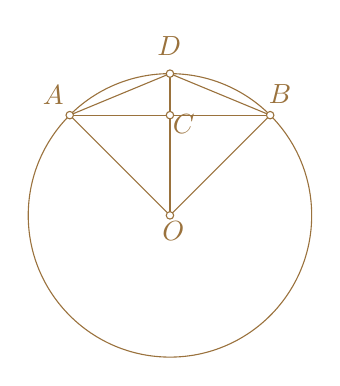
\begin{tikzpicture}[lichsutoanhoc,scale=0.9]
			\draw  (0.,0.) circle (2.cm);
			\draw  (-1.414213562373095,1.4142135623730954)-- (1.4142135623730954,1.4142135623730945);
			\draw  (-1.414213562373095,1.4142135623730954)-- (0.,0.);
			\draw  (0.,0.)-- (1.4142135623730954,1.4142135623730945);
			\draw  (0.,0.)-- (0.,2.);
			\draw  (0.,2.)-- (-1.414213562373095,1.4142135623730954);
			\draw  (0.,2.)-- (1.4142135623730954,1.4142135623730945);
			\draw [fill=white] (0.,0.) circle (1.5pt);
			\draw (0.046257928118391335,-0.21959254276378817) node {$O$};
			\draw [fill=white] (-1.414213562373095,1.4142135623730954) circle (1.5pt);
			\draw (-1.6467653276955618,1.696686527003653) node {$A$};
			\draw [fill=white] (1.4142135623730954,1.4142135623730945) circle (1.5pt);
			\draw (1.5532346723044377,1.7152911781664437) node {$B$};
			\draw [fill=white] (0.,1.414213562373095) circle (1.5pt);
			\draw (0.19509513742071688,1.2873842014222578) node {$C$};
			\draw [fill=white] (0.,2.) circle (1.5pt);
			\draw (-0.00955602536998075,2.3850586200269084) node {$D$};
		\end{tikzpicture}
		\caption{\small\textit{\color{lichsutoanhoc}Hình $3$.}}
		\vspace*{-10pt}
	\end{figure}
	Áp dụng định lý Pythagoras vào tam giác vuông $ACD$  ta có
	\begin{align*}
		A{D^2} = A{C^2} + C{D^2} = A{C^2} + {(OD - OC)^2}.
	\end{align*}
	Lại áp dụng định lý Pythagoras vào tam giác vuông $ACO$  ta được
	\begin{align*}
		OC = \sqrt {O{A^2} - A{C^2}} .
	\end{align*}
	Suy ra 
	\begin{align*}
		A{D^2} = A{C^2} + {\left( {OD - \sqrt {O{A^2} - A{C^2}} } \right)^2}
	\end{align*}
	Với  $OA = OD = 1,\;AC = \dfrac{{{s_n}}}{2},\;AD = {s_{2n}},$ ta có
	\begin{align*}
		&s_{2n}^2 = {\left( {\dfrac{{{s_n}}}{2}} \right)^2} + {\left( {1 - \sqrt {1 - {{\left( {\dfrac{{{s_n}}}{2}} \right)}^2}} } \right)^2}\\
		\implies  &s_{2n}^2 = 2 - \sqrt {4 - s_n^2}.
	\end{align*}
	Suy ra 
	\begin{align*}
		{s_{2n}} = \sqrt {2 - \sqrt {4 - s_n^2} }. \tag{$4$}
	\end{align*}
	Sử dụng công thức ($4$), với hình lục giác đều có cạnh bằng bán kính và bằng $1$ (Hình $4$) ta được 
	\begin{align*}
		{s_{12}} = \sqrt {2 - \sqrt {4 - 1} }  = \sqrt {2 - \sqrt 3 } .
	\end{align*}
	Gấp đôi số cạnh được $n= 12$ thì 
	\begin{align*}
		{s_{24}} &= \sqrt {2 - \sqrt {4 - (2 - \sqrt 3 )} }  \\
		&= \sqrt {2 - \sqrt {2 + \sqrt 3 } } .
	\end{align*}
	Tiếp tục với $n = 24$  thì 
	\begin{align*}
		{s_{48}} = \sqrt {2 - \sqrt {2 + \sqrt {2 + \sqrt 3 } } } .
	\end{align*}
	Và với $n = 96$ thì ta được 
	\begin{align*}
		{s_{96}} = \sqrt {2 - \sqrt {2 + \sqrt {2 + \sqrt {2 + \sqrt 3 } } } } .
	\end{align*}
	\begin{figure}[H]
		\vspace*{-10pt}
		\centering
		\captionsetup{labelformat= empty, justification=centering}
		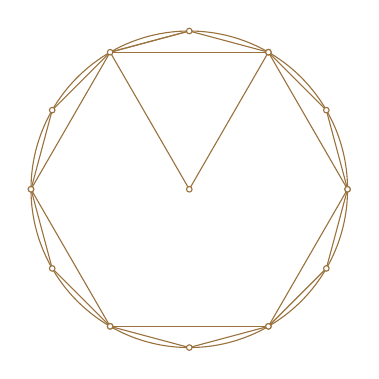
\begin{tikzpicture}[lichsutoanhoc,scale=0.67]
			\draw  (0.,0.) circle (3.cm);
			\draw  (-1.5,2.5980762113533165)-- (1.5,2.5980762113533165);
			\draw  (1.5,2.5980762113533165)-- (3.,0.);
			\draw  (3.,0.)-- (1.5,-2.5980762113533165);
			\draw  (1.5,-2.5980762113533165)-- (-1.5,-2.5980762113533165);
			\draw  (-1.5,-2.5980762113533165)-- (-3.,0.);
			\draw  (-3.,0.)-- (-1.5,2.5980762113533165);
			\draw  (0.,0.)-- (1.5,2.5980762113533165);
			\draw  (-1.5,2.5980762113533165)-- (0.,0.);
			\draw  (-1.5,2.5980762113533165)-- (0.,3.);
			\draw  (0.,3.)-- (-1.5,2.5980762113533165);
			\draw  (-1.5,2.5980762113533165)-- (-2.598076211353315,1.5);
			\draw  (-2.598076211353315,1.5)-- (-3.,0.);
			\draw  (-3.,0.)-- (-2.5980762113533165,-1.5);
			\draw  (-2.5980762113533165,-1.5)-- (-1.5,-2.5980762113533133);
			\draw  (-1.5,-2.5980762113533133)-- (0.,-3.);
			\draw  (0.,-3.)-- (1.5,-2.598076211353315);
			\draw  (1.5,-2.598076211353315)-- (2.598076211353314,-1.5);
			\draw  (2.598076211353314,-1.5)-- (3.,0.);
			\draw  (3.,0.)-- (2.5980762113533165,1.5);
			\draw  (2.5980762113533165,1.5)-- (1.5,2.5980762113533147);
			\draw  (1.5,2.5980762113533147)-- (0.,3.);
				\draw [fill=white] (0.,0.) circle (1.5pt);
				\draw [fill=white] (3.,0.) circle (1.5pt);
				\draw [fill=white] (-3.,0.) circle (1.5pt);
				\draw [fill=white] (-1.5,-2.5980762113533165) circle (1.5pt);
				\draw [fill=white] (1.5,2.5980762113533165) circle (1.5pt);
				\draw [fill=white] (-1.5,2.5980762113533165) circle (1.5pt);
				\draw [fill=white] (1.5,-2.5980762113533165) circle (1.5pt);
				\draw [fill=white] (0.,3.) circle (1.5pt);
				\draw [fill=white] (-2.598076211353315,1.5) circle (1.5pt);
				\draw [fill=white] (-3.,0.) circle (1.5pt);
				\draw [fill=white] (-2.5980762113533165,-1.5) circle (1.5pt);
				\draw [fill=white] (-1.5,-2.5980762113533133) circle (1.5pt);
				\draw [fill=white] (0.,-3.) circle (1.5pt);
				\draw [fill=white] (1.5,-2.598076211353315) circle (1.5pt);
				\draw [fill=white] (2.598076211353314,-1.5) circle (1.5pt);
				\draw [fill=white] (3.,0.) circle (1.5pt);
				\draw [fill=white] (2.5980762113533165,1.5) circle (1.5pt);
				\draw [fill=white] (1.5,2.5980762113533147) circle (1.5pt);
		\end{tikzpicture}
		\caption{\small\textit{\color{lichsutoanhoc}Hình $4$.}}
		\vspace*{-5pt}
	\end{figure}
	Tỷ số chu vi của đa giác đều $96$ cạnh nội tiếp so với đường kính hình tròn  bằng
	\begin{align*}
		&96\cdot\dfrac{{{s_{96}}}}{2} \\[-1ex]
		= \,\,&48\cdot{s_{96}} = 48\sqrt {2 \!-\! \sqrt {2 \!+\! \sqrt {2 \!+\! \sqrt {2 \!+\! \sqrt 3 } } } }  \\[-0.4ex]
		\approx\,\, &3{,}14103 \approx 3\dfrac{{10}}{{71}}.
	\end{align*}
	Tương tự cho đa giác đều ngoại tiếp, ta có 
	\begin{align*}
		{S_{2n}} = \dfrac{{2\sqrt {4 + S_n^2}  - 4}}{{{S_n}}}. \tag{$5$}
	\end{align*}
	Bắt đầu với một lục giác đều ngoại tiếp một đường tròn (Hình $5$).  Do tam giác  $OAB$ đều nên 
	\begin{align*}
		OA = OB = AB = {S_6};\;\;AC = \dfrac{{{S_6}}}{2};\;\;OC = 1.
	\end{align*}
	Áp dụng định lý Pythagoras cho tam giác vuông $OAC$ ta có
	\begin{align*}
		O{A^2} = O{C^2} + A{C^2} &\implies  S_6^2 = {1^2} + {(\dfrac{{{S_6}}}{2})^2} \\[-0.4ex]
		&\implies {S_6} = \dfrac{{2\sqrt 3 }}{3}.
	\end{align*}
	Theo ($5$) ta sẽ tính được ${S_{12}},{S_{24}},{S_{48}},{S_{96.}}$
	Tỷ số chu vi của đa giác đều $96$ cạnh ngoại tiếp so với đường kính hình tròn  là  
	\begin{align*}
		96.\dfrac{{{S_{96}}}}{2} \approx 3{,}14271 \approx 3\dfrac{{10}}{{70}}.
	\end{align*}
	\begin{figure}[H]
		\vspace*{-10pt}
		\centering
		\captionsetup{labelformat= empty, justification=centering}
		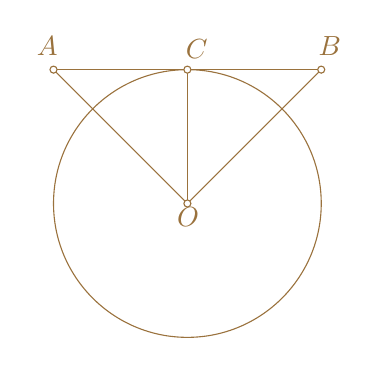
\begin{tikzpicture}[lichsutoanhoc,scale=0.85]
			\draw  (0.,0.) circle (2.cm);
			\draw  (-2.,2.)-- (0.,0.);
			\draw  (0.,0.)-- (2.,2.);
			\draw  (-2.,2.)-- (2.,2.);
			\draw  (0.,2.)-- (0.,0.);
			\draw [fill=white] (0.,0.) circle (1.5pt);
			\draw (0.009048625792809947,-0.20098789160099748) node {$O$};
			\draw [fill=white] (2.,2.) circle (1.5pt);
			\draw (2.129978858350949,2.347849317701327) node {$B$};
			\draw [fill=white] (-2.,2.) circle (1.5pt);
			\draw (-2.093276955602539,2.347849317701327) node {$A$};
			\draw [fill=white] (0.,2.) circle (1.5pt);
			\draw (0.1392811839323448,2.3106400153757454) node {$C$};
		\end{tikzpicture}
		\caption{\small\textit{\color{lichsutoanhoc}Hình $5$.}}
		\vspace*{-10pt}
	\end{figure}
	Vì hình tròn bị giới hạn bởi các đa giác đều nội tiếp và ngoại tiếp, nên ($1$) được chứng minh.
	Trong \textit{Plinthides and Cylinders}, Archimedes còn tính số Pi: 
	\begin{align*}
		\dfrac{{195888}}{{62351}} > \pi  > \dfrac{{211875}}{{67441}}
	\end{align*}
	hay 
	\begin{align*}
		3{,}14697 > \pi  > 3{,}1463911.
	\end{align*}
	Đánh giá này không chính xác vì $\pi  \approx 3{,}141592654$   nằm ngoài khoảng trên. 
	Một đánh giá tinh tế hơn được làm bởi Tannery:
	\begin{align*}
		\dfrac{{195882}}{{62351}} > \pi  > \dfrac{{211872}}{{67441}}
	\end{align*}
	hay 
	\begin{align*}
		3{,}141601578 > \pi  > 3{,}141590427.
	\end{align*}
	Một đánh giá khác là 
	\begin{align*}
		\dfrac{{195888}}{{62351}} > \pi  > \dfrac{{211875}}{{67444}}
	\end{align*}
	hay 
	\begin{align*}
		3{,}141697808 > \pi  > 3{,}141495166.
	\end{align*}
	Khoảng năm $150$ Công nguyên, nhà bác học Ptolemy, trong tác phẩm \textit{Almagest}, dựa trên bảng tính các cung (\textit{Table of Chords}), đã dùng biểu diễn gần đúng số Pi dưới dạng phân số trong hệ đếm cơ số $60$ là 
	\begin{align*}
		\pi  \approx 3 + \dfrac{8}{{60}} + \dfrac{{30}}{{{{60}^2}}} = \dfrac{{377}}{{120}} \approx 3{,}141666667.
	\end{align*}
	Ông cũng nhận xét rằng, số này nằm giữa $3\dfrac{{10}}{{71}}$  và  $3\dfrac{{10}}{{70}}.$
	\vskip 0.1cm
	\textbf{\color{lichsutoanhoc}Số Pi trong toán học Trung Quốc}
	\vskip 0.1cm
	Lúc đầu, người Trung Quốc chấp nhận xấp xỉ $\pi \approx 3$. Đầu thế kỷ II, Trương Hành (張衡, khoảng $78-139$) tìm được  $\pi  \approx \sqrt {10}  \approx 3{,}162$. Bằng cách nội tiếp hình tròn bởi các hình lục giác đều và gấp đôi số cạnh, Lưu Huy  (劉徽, $220-280$) năm $263$ trong cuốn sách Cửu \textit{chương toán thuật} (九章算術) đã tìm được $\pi  \approx 3{,}14$  và sau đó ông tìm được  $\pi  \approx 3{,}14159.$ Tổ Xung Chi (祖沖之, $429-500$), sử dụng thuật toán của Lưu Huy với đa giác $12288 = 3.{2^{12}}$  cạnh, đã tính số $\pi$  chính xác đến $8$ chữ số:
	\begin{align*}
		3{,}1415926 < \;\pi \; < 3{,}1415927\;
	\end{align*}
	Và ông chọn $\pi \; \approx \dfrac{{\;355}}{{113}} \approx 3{,}1415929$
	hoặc  $\pi \; \approx \;\dfrac{{22}}{7} \approx 3{,}145927$. 
	\vskip 0.1cm
	\textbf{\color{lichsutoanhoc}Số Pi trong toán học Việt Nam}
	\vskip 0.1cm
	Lương Thế Vinh ($1441-1497$, [$4$]) và các nhà toán học sau ông, cho đến thế kỉ XVIII, chọn $\pi = 3$.  Nguyễn Hữu Thận ($1757-1831$, [$3$]) đã sử dụng giá trị của số $\pi$ gần đúng đến $8$ chữ số thập phân. Ông đã sử dụng số $\pi  \approx 3{,}14159265$,  trong khi sách \textit{Bút toán chỉ nam} của Nguyễn Cẩn in năm $1909$ [$1$], sau Nguyễn Hữu Thận $80$ năm vẫn dùng số  $\pi$  bằng $3{,}14$ hoặc $3{,}1416$. Tương tự, Phạm Gia Kỉ, trong \textit{Đại thành toán học chỉ minh} [$2$] viết khoảng $1840$ cũng chỉ dùng $\pi$  bằng $3{,}14$ hoặc $3{,}1416$.  Nguyễn Hữu Thận và Nguyễn Cẩn cũng nhắc đến \textit{cách tính của Tây phương} (phương pháp gấp đôi số cạnh của Archimedes). Quan hệ giữa đường kính và chu vi (thông qua số  $\pi$) được Nguyễn Hữu Thận gọi là \textit{định luật chu vi đường kính}. Nguyễn Hữu Thận phát biểu:
	\vskip 0.1cm
	\textbf{\color{lichsutoanhoc}Định luật chu vi đường kính}
	\vskip 0.1cm
	Đường kính $100000000$, chu vi $314159265$
	\vskip 0.1cm
	Lại có chu vi $p = 100000000$, đường kính $d = 31830988$.
	\vskip 0.1cm
	\textit{Giải thích.} Nếu lấy $\pi = 3{,}14159265$, đường kính $d = 100000000$ thì chu vi đường tròn là  $p = d.\pi = 314159265$ (chính xác đến $8$ chữ số).
	\vskip 0.1cm
	Nếu biết chu vi $p = 100000000$,  thì 
	\begin{align*}
		d = \dfrac{p}{\pi } = \dfrac{{1000000}}{{3{,}14159265}} \approx 31830988
	\end{align*}
	(chính xác đến $8$ chữ số).
	\vskip 0.1cm
	Nguyễn Hữu Thận viết: \textit{Phương pháp là cho bên trong hình tròn bao chứa hình vuông, lại từ bên ngoài hình tròn cắt hình vuông. Phép toán đến ức, vạn lần, tập trung tìm sẽ được vô số đầu mối. Trong ngoài đến tập hợp, trong là cạnh huyền chính, ngoài là đường thẳng được cắt. Cho đến vô số đường bao quanh hình tròn, gần giống như trực tuyến mà được số chu vi này, vốn xuất phát từ phép Tây là kỹ lưỡng nhất.}
	\vskip 0.1cm
	\textit{Giải thích}. Đây là phép tính chu vi đường tròn bắt đầu bằng hình vuông nội và ngoại tiếp, sau đó gấp đôi số cạnh (phương pháp của Lưu Huy). 
	Gọi $d$ là đường kính hình tròn, bán kính $r = \dfrac{d}{2}$. Chu vi hình vuông ngoại tiếp bằng $4d > \pi d = 3{,}14$ $d$
	(cạnh hình vuông bằng đường kính). 	
	\begin{figure}[H]
		\vspace*{-5pt}
		\centering
		\captionsetup{labelformat= empty, justification=centering}
		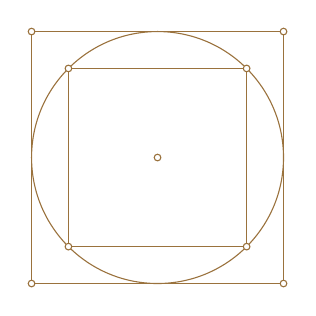
\begin{tikzpicture}[lichsutoanhoc,scale=0.8]
			\draw  (0.,0.) circle (2.cm);
			\draw  (-2.,-2.)-- (2.,-2.);
			\draw  (2.,-2.)-- (2.,2.);
			\draw  (2.,2.)-- (-2.,2.);
			\draw  (-2.,2.)-- (-2.,-2.);
			\draw  (-1.414213562373095,-1.4142135623730954)-- (1.414213562373095,-1.414213562373095);
			\draw  (-1.414213562373095,1.4142135623730954)-- (-1.414213562373095,-1.4142135623730954);
			\draw  (-1.414213562373095,1.4142135623730954)-- (1.4142135623730954,1.4142135623730945);
			\draw  (1.4142135623730954,1.4142135623730945)-- (1.414213562373095,-1.414213562373095);
				\draw [fill=white] (0.,0.) circle (1.5pt);
				\draw [fill=white] (-2.,-2.) circle (1.5pt);
				\draw [fill=white] (2.,-2.) circle (1.5pt);
				\draw [fill=white] (2.,2.) circle (1.5pt);
				\draw [fill=white] (-2.,2.) circle (1.5pt);
				\draw [fill=white] (-1.414213562373095,1.4142135623730954) circle (1.5pt);
				\draw [fill=white] (1.4142135623730954,1.4142135623730945) circle (1.5pt);
				\draw [fill=white] (-1.414213562373095,-1.4142135623730954) circle (1.5pt);
				\draw [fill=white] (1.414213562373095,-1.414213562373095) circle (1.5pt);
		\end{tikzpicture}
		\caption{\small\textit{\color{lichsutoanhoc}Hình $6$.}}
		\vspace*{-10pt}
	\end{figure}
	Hình vuông nội tiếp đường tròn có đường chéo bằng cạnh hình vuông bằng $\dfrac{d}{{\sqrt 2 }} = r\sqrt 2 .$ Do đó  chu vi hình vuông nội tiếp bằng (Hình $6$): $4r\; = 2d\; \approx 2d \times 1{,}4142 \approx 2{,}8284 < d\pi  \approx d.3{,}14 < 4d$.
	Gấp đôi số cạnh đa giác nội ngoại tiếp và tính giới hạn ta được chu vi hình tròn.
	Nguyễn Hữu Thận cũng phát biểu:
	\vskip 0.1cm
	\textbf{\color{lichsutoanhoc}Phép rút gọn chu vi, đường kính}
	\vskip 0.1cm 
	Đường kính: $113$;	Chu vi: $355$
	\vskip 0.1cm
	Suy luận ban đầu là: Phép tính chu vi, đường kính, cách làm tốt dùng đường kính là $7$, đường bao quanh (chu vi) là $22$ thì thừa. Cách tỉ mỉ dùng đường kính là $50$, chu vi là $157$ thì thiếu. Chỉ có sắp đặt đường kính gộp lại là $113$, chu vi là $355$, phù hợp với định luật hơn. Cho nên chọn dùng nó.
	\vskip 0.1cm 
	\textit{Giải thích}. Chu vi hình tròn bằng:
	\begin{align*}
		p = d\pi  &\approx 7 \times 3{,}14159265 \\
		&\approx 21.99114855 < 22;\\
		p = d\pi  &\approx 50 \times 3{,}14159265 \\
		&\approx 157.0796325 > 157.\\
		p=d\pi  &\approx 113 \times 3{,}14159265 \\
		&\approx 354.99996945 < 355.
	\end{align*}
	Sai số:
	\vskip 0.1cm 		
	$1)$ $22 - 21{,}99114855 = 0{,}00885415$;  
	\vskip 0.1cm
	$2)$ $157{,}0796325 - 157 = 0{,}0796325$;
	\vskip 0.1cm
	$3)$ $355 - 354{,}99996 = 0{,}00004$
	($\dfrac{{355}}{{113}}$ chính xác nhất, đến $4$ chữ số).
	\vskip 0.1cm
	Vậy chọn $\pi  \approx \dfrac{{355}}{{113}}$ là phân số chính xác hơn cả. 
	\vskip 0.1cm
	Nguyễn Hữu Thận viết: \textit{Cạnh hình vuông với đường kính hình tròn bằng nhau nhưng diện tích hình vuông và diện tích hình tròn không có cùng định luật.}
	\vskip 0.1cm
	Diện tích hình vuông: $100000000$.
	\vskip 0.1cm	
	Diện tích hình tròn: $78539816$.
	\vskip 0.1cm
	Mặt khác:
	\vskip 0.1cm
	Diện tích hình tròn: $100000000$.
	\vskip 0.1cm 	
	Diện tích hình vuông: $127323954$.
	\vskip 0.1cm
	\textit{Giải thích.} Với cạnh $a = 10000$ thì diện tích hình vuông ${a^2} = 100000000$. Diện tích hình tròn nội tiếp hình vuông có đường kính bằng cạnh hình vuông do đó bằng 
	\setlength{\abovedisplayskip}{7pt}
	\setlength{\belowdisplayskip}{7pt}
	\begin{align*}
			S &= \pi {R^2} = \dfrac{{\pi {d^2}}}{4} = \dfrac{{\pi {a^2}}}{4}\\
			&\approx 3{,}14159265 \times 100000000:4 \\
			&\approx 78539816.	
	\end{align*}
	Nếu diện tích hình tròn là $100000000$ thì diện tích hình vuông là
	\begin{align*}
		{a^2} &= \dfrac{{4S}}{\pi } = \dfrac{{4 \times 100000000}}{{3{,}14159265}}\\ &= 127323954.
	\end{align*}
	Nguyễn Hữu Thận viết:  \textit{Diện tích hình vuông và diện tích hình tròn bằng nhau, cạnh hình vuông và đường kính hình tròn không cùng định luật.}
	\vskip 0.1cm
	Đường kính hình tròn: $100000000$.
	\vskip 0.1cm 
	Cạnh hình vuông: $88622692$.
	\vskip 0.1cm
	Lại có: 
	\vskip 0.1cm
	Cạnh hình vuông: $100000000$.
	\vskip 0.1cm 
	Đường kính hình tròn: $112837916$.
	\vskip 0.1cm
	\textit{Giải thích}. Diện tích hình vuông bằng diện tích hình tròn và bằng 
	\begin{align*}
		S &= \pi {R^2} = \dfrac{{\pi {d^2}}}{4}\\
		&\approx 3{,}14159265 \times {100000000^2}:4 \\
		&\approx 7853981633974483.
	\end{align*}
	Cạnh $a$ của hình vuông bằng
	\begin{align*}
		a = \sqrt S  \approx 88622692.
	\end{align*}
	Tương tự, nếu có cạnh hình vuông bằng $100000000$ thì  
	\begin{align*}
		d &= \sqrt {\dfrac{{4S}}{\pi }}  = \sqrt {\dfrac{{4{a^2}}}{\pi }}  = \dfrac{{2a}}{{\sqrt \pi  }} \\
		&\approx \dfrac{{2 \times 100000000}}{{\sqrt {3{,}14159265} }} \\
		&\approx 112837916.
	\end{align*}
	Như vậy, có thể khẳng định Nguyễn Hữu Thận ($1757-1831$) là người Việt Nam đầu tiên có cảm nhận toán học về số vô tỷ và giới hạn thông qua quan hệ giữa số $\pi$ và diện tích các đa giác đều nội ngoại tiếp hình tròn khi gấp đôi số cạnh.
	\vskip 0.1cm
	\textbf{\color{lichsutoanhoc}Tiếp tục tính gần đúng số Pi}
	\vskip 0.1cm
	Tính toán thiên văn trong \textit{Shatapatha Brahmana} (Ấn Độ, thế kỉ IV trước Công nguyên) dùng xấp xỉ $\pi  \approx \dfrac{{339}}{{108}} \approx \;3{,}139$.  Một số tư liệu cổ của Ấn Độ chọn $\pi  \approx \sqrt {10}  \approx 3{,}162$. Trong tác phẩm \textit{Āryabhaṭīya}, nhà thiên văn Ấn Độ Aryabhata ($476-550$) đã sử dụng giá trị $\pi  = 3{,}1416$.
	\vskip 0.1cm 
	Fibonacci vào năm $1220$ đã tính được $\pi  = 3{,}1418$  độc lập với Archimedes. 
	\vskip 0.1cm
	Tác giả người Ý Dante đã sử dụng giá trị  $\pi  = 3 + \dfrac{{\sqrt 2 }}{{10}} \approx 3{,}14142.$
	\vskip 0.1cm 
	Mãi $8$ thế kỷ sau, kỷ lục của Tổ Xung Chi mới bị phá bởi nhà toán học Ba Tư Al--Kāshānī ($1370-1450$). Ông dùng phương pháp của Archimedes và xét các đa giác đều $3.2^{28}$ cạnh nội tiếp và ngoại tiếp đường tròn và tìm được số $\pi$ đúng tới $17$ chữ số là $3{,}1415926535897932$.  Al--Kāshānī còn dự đoán $\pi$ là số vô tỷ. Điều này chỉ được chứng minh bởi nhà toán học Thụy Sĩ Johann Heinrich Lambert ($1728 - 1777$).
	\vskip 0.1cm 
	Cũng gấp đôi số cạnh như Archimedes, nhưng xuất phát từ hình vuông, nhà toán học Pháp François Viète vào năm $1578$ đã tính chính xác số $\pi$  đến $9$ chữ số nhờ sử dụng đa giác  $3 \times 2^{17}$ cạnh dựa trên công thức
	\begin{align*}
			\dfrac{2}{\pi } = &\cos \dfrac{\pi }{4} \cdot \cos \dfrac{\pi }{8} \cdot \cos \dfrac{\pi }{{16}}...\\
			= &\sqrt {\dfrac{1}{2}}  \cdot \sqrt {\dfrac{1}{2}\left( {1 + \sqrt {\dfrac{1}{2}} } \right)}  \\
			 &\!\times\!\sqrt {\dfrac{1}{2}\left( {1 \!+\! \sqrt {\dfrac{1}{2}\left(\! {1 \!+\! \sqrt {\dfrac{1}{2}} } \!\right)} } \right)} ... \tag{$6$}
	\end{align*}
	\textit{Giải thích}: Sử dụng công thức ${\cos ^2}a = \dfrac{{1 + \cos 2a}}{2}$  và $\cos \dfrac{\pi }{4} = \sqrt {\dfrac{1}{2}},$ ta dễ dàng tính được 
	\begin{align*}
		\cos \dfrac{\pi }{8} &= \sqrt {\dfrac{1}{2}\left( {1 + \sqrt {\dfrac{1}{2}} } \right)};\\
		\cos \dfrac{\pi }{{16}} &= \sqrt {\dfrac{1}{2}\left( {1 + \sqrt {\dfrac{1}{2}\left( {1 + \sqrt {\dfrac{1}{2}} } \right)} } \right)}.
	\end{align*}
	Công lao của François Viète là phát hiện ra công thức biểu diễn ($6$).
	\vskip 0.1cm
	Gọi $A(n)$  là diện tích đa giác đều $n$  cạnh nội tiếp hình tròn bán kính  $r$ và $\beta$ là góc ở tâm.  Ta có (Hình $2$):
	\begin{align*}
		A(n) = n\dfrac{1}{2}{r^2}\sin 2\beta  = n{r^2}\sin \beta \cos \beta .
	\end{align*}
	Tương tự,  
	\begin{align*}
		A(2n) = 2n\dfrac{1}{2}{r^2}\sin \beta  = n{r^2}\sin \beta .
	\end{align*}
	Suy ra
	\begin{align*}
		\dfrac{{A(n)}}{{A(4n)}} = \dfrac{{A(n)}}{{A(2n)}}\cdot\dfrac{{A(2n)}}{{A(4n)}} = \cos \beta \cos \dfrac{\beta }{2}.
	\end{align*}
	Do đó,
	\begin{align*}
			\dfrac{{A(n)}}{{A({2^k}n)}} &= \dfrac{{A(n)}}{{A(2n)}}\cdot\dfrac{{A(2n)}}{{A(4n)}}...\dfrac{{A\left( {{2^{k - 1}}n} \right)}}{{A({2^k}n)}}\\
			&= \cos \beta \cos \dfrac{\beta }{2}...\cos \dfrac{\beta }{{{2^k}}}.
	\end{align*}
	Khi $k$  tiến tới $\infty$  thì $A({2^k}n)$  tiến tới diện tích hình tròn, nghĩa là $\mathop {\lim }\limits_{k \to \infty } A({2^k}n) = \pi {r^2}.$ Suy ra  
	\begin{align*}
		\pi {r^2} &= \dfrac{{A(n)}}{{\cos \beta \cos \dfrac{\beta }{2}...\cos \dfrac{\beta }{{{2^k}}}...}} \\
		&= \dfrac{{\dfrac{1}{2}n{r^2}\sin 2\beta }}{{\cos \beta \cos \dfrac{\beta }{2}...\cos \dfrac{\beta }{{{2^k}}}...}}.
	\end{align*}
	Vậy  
	\begin{align*}
		\pi  = \dfrac{{n\sin 2\beta }}{{2\cos \beta \cos \dfrac{\beta }{2}...\cos \dfrac{\beta }{{{2^k}}}...}}.
	\end{align*}
	Để được công thức ($6$), Viète đã chọn $n = 4$. Khi ấy $\beta  = \dfrac{\pi }{4}$  và 
	\begin{align*}
		\sin 2\beta  = \sin \dfrac{\pi }{2} = 1, \cos \beta  = \cos \dfrac{\pi }{4} = \dfrac{1}{{\sqrt 2 }}.
	\end{align*}
	Nhà toán học Đức Adriaan van Roomen ($1561-1615$) nhận được xấp xỉ số  $\pi$ đến $15$ chữ số vào năm $1593$.
	\vskip 0.1cm 
	Năm $1596$, nhà toán học người Hà Lan Ludolph van Ceulen ($1540-1610$) đã dành $50$ năm trong hơn $70$ năm của đời mình để tính số $\pi$   xấp xỉ đến $35$ chữ số.
	\vskip 0.1cm 
	Năm $1621$, nhà khoa học Đức Willebrord Snellius đã đạt được xấp xỉ số $\pi$  đến $34$ chữ số.
	\vskip 0.1cm
	Năm $1630$, nhà thiên văn người Áo Christoph Grienberger ($1561-1636$) đã tìm được số $\pi$ xấp xỉ đến $38$ chữ số bằng cách sử dụng đa giác đều  $10^{40}$ cạnh.
	\vskip 0.1cm 
	Năm $1654$, Christiaan Huygens đã nhận được xấp xỉ đến $10$ chữ số thập phân nhờ sử dụng phương pháp ngoại suy Richardson.  
	\vskip 0.1cm
	Kỉ lục Christoph Grienberger chỉ bị vượt qua và thuật toán Archimedes đi vào lịch sử khi năm $1699$, số  $\pi$ được tính gần đúng đến $71$ chữ số nhờ phân tích số  $\pi$ dưới dạng chuỗi lũy thừa. Từ đó, số $\pi$ được tính gần đúng nhờ công cụ giải tích. Điều này sẽ được trình bày chi tiết trong Phần $2$.
	\vskip 0.1cm 
	\textbf{\color{lichsutoanhoc}Biểu diễn số $\pmb{\pi}$  dưới dạng phân số liên tục}
	\vskip 0.1cm
	Số $\pi$  có thể biểu diễn dưới dạng phân số liên tục như sau: 
	\begin{align*}
		\pi  \!=\! 3 \!+\! \dfrac{1}{{7 \!+\! \dfrac{1}{{15 \!+\! \dfrac{1}{{1 \!+\! \dfrac{1}{{292 \!+\! \dfrac{1}{{1 \!+\! \dfrac{1}{{1 \!+\! \dfrac{1}{{1 \!+\! ...}}}}}}}}}}}}}}
	\end{align*}
	Cắt cụt phân số này ta lần lượt được  $\pi  \approx 3;$  $\pi  \approx 3 + \dfrac{1}{7} = \dfrac{{22}}{7};$ $\pi  = 3 + \dfrac{1}{{7 + \dfrac{1}{{15}}}} = 3 + \dfrac{{15}}{{106}} = \dfrac{{333}}{{106}};$ $\pi  = 3 + \dfrac{1}{{7 + \dfrac{1}{{15 + 1}}}} = 3 + \dfrac{{16}}{{113}} = \dfrac{{355}}{{113}},$
	là các phân số xấp xỉ số $\pi$ thường gặp trong lịch sử các dân tộc Tây--Đông.
	\vskip 0.1cm
	\textbf{\color{lichsutoanhoc}Thông tin tác giả}
	\vskip 0.1cm
	$\bullet$ Tạ Duy Phượng (PGS Toán học)
	\vskip 0.1cm
	$\bullet$ Đoàn Thị Lệ, Cung Thị Kim Thành (Thạc sĩ Hán Nôm)
	\vskip 0.1cm
	$\bullet$ Mai Văn Thu, Nguyễn Hoàng Vũ (Thạc sĩ Toán học)
	\vskip 0.1cm
	\textbf{\color{lichsutoanhoc}Tài liệu trích dẫn}
	\vskip 0.1cm
	[$1$]   阮菫 Nguyễn Cẩn ($1909$),  \textit{Bút toán chỉ nam}, Thư viện viện nghiên cứu Hán Nôm, Viện nghiên cứu Hán Nôm, VHv. $282$ và A.$1031$. Bản thảo bản dịch của Đoàn Thị Lệ, $2015$.
	\vskip 0.1cm
	[$2$] 范嘉紀  Phạm Gia Kỷ,  大成算學指明  \textit{Đại thành toán học chỉ minh}, Thư viện viện nghiên cứu Hán Nôm, Viện nghiên cứu Hán Nôm, A.$1555$. Bản thảo bản dịch của Phạm Hữu Lộc, $2019$.
	\vskip 0.1cm 
	[$3$]  阮 有 慎 Nguyễn Hữu Thận,  意齋算法一得錄  \textit{Ý Trai toán pháp nhất đắc lục} ($1829$), Thư viện Viện nghiên cứu Hán Nôm, Vhv.$1184$, A.$1336$, A. $982$, A.$1336$/a. Bản thảo bản dịch của Đoàn Thị Lệ và Cung Thị Kim Thành, $2015-2016$.
	\vskip 0.1cm 
	[$4$] 梁世榮  Lương Thế Vinh,  算法大成 \textit{Toán pháp đại thành}, Thư viện Viện nghiên cứu Hán Nôm, Ký hiệu: A.$2931$ và VHv. $1152$. Bản thảo bản dịch của Cung Thị Kim Thành, $2017$.
	\vskip 0.1cm
	[$5$] David M. Burton, \textit{The History of Mathematics, An Introduction}, Seventh Edition, McGraw Hill, $2011$, $819$ p.
	\vskip 0.1cm
	[$6$] Heinrich Dörrie, \textit{The $100$ Great Problems of Elementary Mathematics, Their History and Solution}, New York, Dover Publications, INC., $1965$.
	\vskip 0.1cm     
	[$7$] Thomas Heath, \textit{A History of Greek Mathematics}, Oxford at the Clarendon Press, $1921$, Volume $1$, $232-235$.
	\vskip 0.1cm
	[$8$] Lam Lay--Yong and Ang Tian--Se, Circle Measurements in Ancient China, \textit{Historia Mathematica}, $13$,  ($1986$), $325-340$.
	\vskip 0.1cm
	[$9$] A. Volkov, Calculation of $\pi$ in ancient China: From Liu Hui to Zu Chongzhi, \textit{Historia Scientiarum}, Vol. $4$ ($1994$), No $2$, $139-157$. 
	\vskip 0.1cm
	\hfill (\textit{Còn tiếp})
\end{multicols}
%	\newpage
%
%	\setcounter{figure}{0}
%	\thispagestyle{timhieukhoahocnone}
\pagestyle{timhieukhoahoc}
\everymath{\color{timhieukhoahoc}}
\blfootnote{$^1$\text{\color{timhieukhoahoc}Hà Nội.}}
\graphicspath{{../timhieukhoahoc/pic2/}}
\begingroup
\AddToShipoutPicture*{\put(0,616){\includegraphics[width=19.3cm]{../bannertimhieu}}}
\AddToShipoutPicture*{\put(112,525){\includegraphics[scale=1]{../tieude.pdf}}}
\centering
\endgroup
\vspace*{178pt}

\begin{multicols}{2}
	Hiện tượng cộng hưởng là một nội dung kiến thức quan trọng trong chương trình vật lý lớp $12$. Nó xảy ra khi tác động từ bên ngoài có một tần số phù hợp làm biên độ của dao động bị tăng vọt. Trong bài viết này, chúng ta hãy cùng tìm hiểu về quá trình phát hiện của hiện tượng cộng hưởng cũng như một số ứng dụng thú vị của nó.
	\vskip 0.1cm
	$\pmb{1.}$ \textbf{\color{timhieukhoahoc}Mô hình cho thủy triều và bài toán dao động cưỡng bức}
	\vskip 0.1cm
	Hiện tượng cộng hưởng xuất hiện lần đầu tiên trong các tài liệu khoa học khi Galileo tiến hành giải thích về hiện tượng mang tính chu kỳ của thủy triều dựa trên các quan sát về dao động. Ông nhận thấy rằng một tác động yếu có thể làm tăng mạnh biên độ của một dao động nếu tác động này có một tần số phù hợp. Một ví dụ mà Galileo đưa ra là việc một quả chuông sau khi được một người tiến hành rung thì dây thừng của nó có thể nhấc bổng tận $6$ người lên. Sự tăng biên độ nhờ các tác động mang tính chu kỳ cũng có thể thấy được ở con lắc đơn trong đồng hồ hay các nhạc cụ dây.
	\vskip 0.1cm
	Galileo đưa ra một nhận định đúng đắn rằng mỗi một hệ dao động có một tần số dao động tự nhiên (dao động tự do). Tuy nhiên, ông lại cho rằng nó chỉ có thể có thể dao động với tần số này mà thôi (nhận định này không đúng). Sai lầm trên là một trong những nguyên nhân khiến Galileo kết luận rằng thủy triều được gây ra bởi chuyển động của Trái đất trong khi thực tế thì Mặt trăng có vai trò quan trọng liên quan đến chu kỳ của hiện tượng này.
	\vskip 0.1cm
	Phải đến thế kỷ $18$, tính chu kỳ của thủy triều lại được tiếp tục nghiên cứu bởi Euler. Ông đã tiến hành giải phương trình dao động với ngoại lực cũng là một hàm có chu kỳ. Bằng các công cụ giải tích, Euler đã tìm ra rằng nghiệm của trường hợp này là tổng của hai dao động điều hòa với hai tần số khác nhau. Tần số thức nhất phụ thuộc vào các tham số cấu tạo của hệ dao động và tần số thứ hai là tần số của ngoại lực. Euler giải được nghiệm đúng cho trường hợp hai tần số này bằng nhau và công thức nghiệm của ông cũng cho thấy sự tăng biên độ tuyến tính theo thời gian (tức khi cộng hưởng xảy ra). Tuy vậy, Euler không tiếp tục đi sâu vào phương diện vật lý của vấn đề này, ngoài việc nhắc đến sự liên hệ giữa nó và thủy triều. Trong các công trình sau này về cơ học, Euler cũng không quay lại bài toán trên, có thể là do ông chỉ xem nó như một câu hỏi toán học thú vị mà thôi.
	\vskip 0.1cm
	Đến thế kỷ $19$, Thomas Young, sau khi tiến hành thí nghiệm chứng minh bản chất sóng của ánh sáng năm $1802$, cũng bắt đầu nghiên cứu về mô hình của thủy triều. Ông tiến hành giải phương trình dao động dưới tác dụng của ngoại lực có chu kỳ giống như Euler nhưng thêm vào thành phần biểu diễn lực cản. Đồng thời, Young cũng đưa ra thuật ngữ dao động cưỡng bức để gọi tên trường hợp dao động này. Tuy nhiên, ông cũng vẫn chủ yếu tập trung vào giải thích tính chu kỳ của thủy triều mà không tiến hành mở rộng sang các ứng dụng cơ học khác. Khi các mô hình mới trong không gian $3$ chiều được đưa ra cho thủy triều thì mô hình dao động cưỡng bức của con lắc không còn được sử dụng nữa và nghiên cứu này của Young cũng không được chú ý đến. Đột phá thật sự chỉ xảy ra vài thập kỷ sau với các nghiên cứu của Helmholtz về sự cộng hưởng của sóng âm.
	\vskip 0.1cm
	$\pmb{2.}$ \textbf{\color{timhieukhoahoc}Helmholtz và sự cộng hưởng của sóng âm}
	\begin{figure}[H]
		\centering
		\vspace*{-5pt}
		\captionsetup{labelformat= empty, justification=centering}
		\includegraphics[width=1\linewidth]{1}
		\caption{\small\textit{\color{timhieukhoahoc}Hermann von Helmholtz ($1821 - 1894$).}}
		\vspace*{-10pt}
	\end{figure}
	Hermann von Helmholtz, sinh năm $1821$ tại Postdam, nay thuộc Đức, là con trai duy nhất của một giáo viên. Ông muốn học vật lý nhưng do hoàn cảnh tài chính nên theo học quân y bằng học bổng chính phủ. Trong thời gian làm bác sĩ phẫu thuật cho quân đội, Helmholtz vẫn có những đóng góp quan trọng trong vật lý, đặc biệt là sự thiết lập định luật bảo toàn năng lượng. Từ năm $1849$, ông giữ vị trí giáo sư ngành sinh lý học ở nhiều đại học khác nhau cho đến khi trở thành giáo sư vật lý tại đại học Humboldt, Berlin năm $1871$.
	\vskip 0.1cm
	Helmholtz bắt đầu các nghiên cứu về âm thanh vào năm $1856$, dựa trên các ý tưởng toán học của Fourier. Trước đó, khi giải bài toán về phương trình truyền nhiệt, Fourier đã đưa ra phương pháp biểu diễn một hàm số tuần hoàn dưới dạng tổng của các sóng hình sine. Tần số, pha, và biên độ của mỗi sóng trong tổng này phụ thuộc vào các điều kiện ban đầu và điều kiện biên của bài toán. Cách biểu diễn này còn được biết đến với tên gọi chuỗi Fourier.
	\begin{figure}[H]
		\centering
		\vspace*{-5pt}
		\captionsetup{labelformat= empty, justification=centering}
		\includegraphics[width=1\linewidth]{2}
		\caption{\small\textit{\color{timhieukhoahoc}Hình $1$. Một thiết bị cộng hưởng Helmholtz.}}
		\vspace*{-10pt}
	\end{figure}
	Phương pháp của Fourier giúp Helmholtz đưa ra ý tưởng rằng các âm thanh phức tạp có thể được đơn giản hóa thành tổng của các sóng âm đơn giản hơn với các tần số khác nhau. Để tiến hành nghiên cứu vấn đề này, ông đã chế tạo các dụng cụ thí nghiệm được gọi là thiết bị cộng hưởng Helmholtz. Mỗi một thiết bị cộng hưởng Helmholtz gồm một quả cầu kim loại hoặc thủy tinh có lỗ hở ở một đầu. Đầu còn lại có một núm nhỏ để người sử dụng có thể gắn vào tai.
	\vskip 0.1cm
	Cơ chế hoạt động của thiết bị cộng hưởng này có thể được giải thích theo một mô hình tương tự với dao động của con lắc lò xo dựa trên tính đàn hồi của không khí. Khi một khối không khí đi vào hình cầu, nó sẽ đóng vai trò của vật dao động còn lượng không khí có sẵn ở trong thiết bị sẽ bị nén lại. Tương tự như lò xo bị nén, lượng khí bị nén lại này sẽ đẩy khối khi ban đầu ra ngoài xa hơn so với trước, đồng thời giãn nở ra. Do đó, không khí ở trong một vật chứa hình cầu có thể dao động tương tự như một con lắc lò xo.
	\vskip 0.2cm
	\PIbox{Bản thân các dụng cụ âm nhạc đều là các thiết bị cộng hưởng để khuyếch đại âm thanh: ống của các loại kèn, sáo, hộp đàn của các loại đàn dây, thân của các loại trống. 
		\begin{figure}[H]
			\centering
			\vspace*{-5pt}
			\captionsetup{labelformat= empty, justification=centering}
			\includegraphics[width=1\linewidth]{3}
			%		\caption{\small\textit{\color{timhieukhoahoc}Hình $1$. Một thiết bị cộng hưởng Helmholtz.}}
%			\vspace*{-10pt}
	\end{figure}}
	\vskip 0.2cm
	Tùy theo kích thước hình cầu và độ rộng của lỗ, mỗi một thiết bị cộng hưởng Helmholtz có một tần số dao động tự nhiên riêng biệt. Khi sử dụng núm của thiết bị để nghe bằng cách cắm vào tai, người dùng chỉ nghe thấy các thành phần của âm thanh có tần số giống với tần số dao động tự nhiên của thiết bị còn các tần số khác đều bị suy giảm.
	Bản thân các dụng cụ âm nhạc đều là các thiết bị cộng hưởng để khuyếch đại âm thanh: ống của các loại kèn, sáo, hộp đàn của các loại đàn dây, thân của các loại trống. 
	\begin{figure}[H]
		\centering
		\vspace*{-5pt}
		\captionsetup{labelformat= empty, justification=centering}
		\includegraphics[width=1\linewidth]{4}
		\caption{\small\textit{\color{timhieukhoahoc}Hình $2$. Một bộ thiết bị cộng hưởng Helmholtz cho các tần số khác nhau.}}
		\vspace*{-10pt}
	\end{figure}
	Helmholtz không dừng ở việc phân tích âm thanh mà còn tiến hành các thí nghiệm tổng hợp âm thanh. Ông sử dụng các âm thoa được kích hoạt cho dao động bằng nam châm điện. Các âm thoa cấu tạo khác nhau sẽ có các tần số cơ bản khác nhau. Âm thanh của chúng sẽ được khuyếch đại bằng thiết bị cộng hưởng Helmholtz. Thông qua các thí nghiệm phân tích cũng như tổng hợp âm thanh, Helmholtz đã xác định được rằng âm thanh của các dụng cụ âm nhạc cũng như các nguyên âm trong giọng nói của con người là sự tổng hợp của những âm thanh với tần số khác nhau và ta cũng có thể tạo những âm thanh tương tự bằng cách tổng hợp các sóng âm với tần số tương ứng. Ví dụ với nguyên âm ``a”, thanh quản sẽ khuyếch đại các tần số gần với $800$ Hz, $1600$ Hz và $2400$ Hz. Với những nguyên âm khác, các cơ của cổ họng và miệng sẽ thay đổi hình dạng của thanh quản, tạo ra một bộ các tần số cộng hưởng khác. Dựa trên các công trình của Helmholtz, Graham Bell đã nảy sinh ý tưởng về việc truyền dẫn âm thanh trên dây điện theo các tần số khác nhau và tổng hợp lại thành âm thanh ban đầu, dẫn đến sự ra đời của điện thoại cố định.
	\begin{figure}[H]
		\centering
		\vspace*{-5pt}
		\captionsetup{labelformat= empty, justification=centering}
		\includegraphics[width=1\linewidth]{5}
		\caption{\small\textit{\color{timhieukhoahoc}Hình $3$. Thiết bị phát sóng âm của Helmholtz.}}
		\vspace*{-10pt}
	\end{figure}
	Cũng do nghiên cứu của Helmholtz, thuật ngữ ``resonance" chính thức được sử dụng để chỉ sự dao động mãnh liệt ở một tần số đặc thù, tất nhiên lúc này vẫn chỉ giới hạn với dao động của sóng âm.
	\begin{figure}[H]
		\centering
		\vspace*{-5pt}
		\captionsetup{labelformat= empty, justification=centering}
		\includegraphics[width=1\linewidth]{6}
		\caption{\small\textit{\color{timhieukhoahoc}Hình $4$. Chim gõ kiến sử dụng thân cây làm thiết bị cộng hưởng.}}
		\vspace*{-10pt}
	\end{figure}
	Không chỉ có con người, một số loài động vật cũng biết sử dụng hiện các vật thể trong tự nhiên làm thiết bị cộng hưởng sóng âm. Các loài chim gõ kiến sử dụng việc gõ vào thân cây để giao tiếp với nhau trong rừng nên chúng thường chọn những thân cây khô và rỗng để tăng hiệu quả cộng hưởng giúp âm thanh vang xa hơn. Trong khi đó, một số loài bướm đêm lại có các cấu trúc vảy trên cánh cộng hưởng với sóng âm mà dơi bắt mồi phát ra, khiến sóng này bị hấp thụ thay vì phản xạ lại cho dơi.
	\begin{figure}[H]
		\centering
		\vspace*{-5pt}
		\captionsetup{labelformat= empty, justification=centering}
		\includegraphics[width=1\linewidth]{7}
		\caption{\small\textit{\color{timhieukhoahoc}Hình $5$. Một số loài bướm đêm có cấu tạo vảy đặc thù cộng hưởng với sóng âm phát ra từ dơi bắt mồi.}}
		\vspace*{-10pt}
	\end{figure}
	$\pmb{3.}$ \textbf{\color{timhieukhoahoc}Cộng hưởng điện từ}
	\vskip 0.1cm
	Ngay khi đang làm việc với hiện tượng sóng âm, Helmholtz cũng giành sự chú ý cho một loại sóng khác trong tự nhiên. Các nghiên cứu khoa học trước đó của Faraday và Weber đã cho thấy khả năng dòng điện cũng là một hiện tượng sóng. Helmholtz cho rằng, nếu toán học có thể mô tả dao động sóng âm trong một ống hình trụ thì những phương trình tương tự cũng có thể biểu diễn chuyển động của các sóng điện trường trong mạch điện kín. Nhiều nhà khoa học đương thời khác cũng có những ý tưởng giống như vậy, bao gồm Kelvin và Maxwell. Với những công trình được công bố trong giai đoạn $1861-1865$, Maxwell đã xây dựng cơ sở toán học cho lý thuyết về sóng điện từ với hệ các phương trình mô tả dao động của các sóng này.
	\vskip 0.1cm
	Trước đó, trong công bố năm $1853$, Kelvin đã chỉ ra sự tăng vọt cường độ dòng điện trong mạch $LC$ (gồm cuộn cảm có độ tự cảm $L$ và tụ điện có điện dung $C$) khi tần số dòng xoay chiều là $\omega =\sqrt{LC}$. Phải đến năm $1885$, nhà vật lý Anton Oberbeck mới sử dụng thuật ngữ cộng hưởng mượn từ lĩnh vực sóng âm để miêu tả hiện tượng này và chỉ ra sự tương đồng về mặt phương trình của hai loại dao động, sóng âm và sóng điện từ. 
	\vskip 0.1cm
	Năm $1886$, Heinrich Hertz phát hiện rằng mạch LC phát ra sóng điện từ trong không gian mà không cần dây dẫn, cung cấp bằng chứng quan trọng khẳng định dự đoán của Maxwell. Đồng thời, thí nghiệm này cũng khẳng định sự tồn tại của cộng hưởng sóng điện từ.
	\vskip 0.1cm
	Bản thân Hertz cho rằng sóng điện từ cũng như đặc tính cộng hưởng của nó không có ứng dụng trong đời sống. Tuy nhiên thực tế lại hoàn toàn ngược lại. Dựa trên công trình của Hertz và một số nhà khoa học khác, Guglielmo Marconi đã chế tạo hệ thống thu phát sóng radio cho phép truyền tín hiệu không dây trong thực tế đồng thời thương mại hóa công nghệ này. Để tránh xung đột từ các nguồn khác nhau, cả thiết bị phát và thiết bị thu được điều chỉnh về cùng một tần số cộng hưởng. Ngày nay việc thu phát sóng không dây đã trở nên quá quen thuộc trong đời sống, từ phát thanh, truyền hình không dây cho đến điện thoại di động, Internet wifi hay các thiết bị bluetooth. Trong các công nghệ này, các mạch cộng hưởng vẫn luôn đóng vai trò thiết yếu khi thu phát tín hiệu.
		\begin{figure}[H]
		\centering
		\vspace*{-5pt}
		\captionsetup{labelformat= empty, justification=centering}
		\includegraphics[width=1\linewidth]{8}
		\caption{\small\textit{\color{timhieukhoahoc}Hình $6$. Marconi và thiết bị thu phát sóng không dây do ông chế tạo.}}
		\vspace*{-5pt}
	\end{figure}
	\PIbox{Một dạng cộng hưởng khác ở cấp độ vi mô hơn là cộng hưởng từ hạt nhân. Khi ta kích thích một hạt nhân được đặt trong một từ trường mạnh, hạt nhân này có thể phát ra bức xạ với tần số nhất định do sự chuyển trạng thái của spin trong hạt nhân. Sự cộng hưởng này được sử dụng để quan sát bên trong các mẫu vật cũng như chụp cắt lớp cộng hưởng từ (MRI) trong y học.
	\begin{figure}[H]
		\centering
		\vspace*{-5pt}
		\captionsetup{labelformat= empty, justification=centering}
		\includegraphics[width=1\linewidth]{9}
		\vspace*{-10pt}
	\end{figure}}
	\vskip 0.2cm
	$\pmb{4.}$ \textbf{\color{timhieukhoahoc}Cộng hưởng và cơ học ứng dụng}
	\vskip 0.1cm
	Quá trình để lý thuyết cộng hưởng được chấp nhận trong cơ học ứng dụng kéo dài suốt từ thế kỷ $19$ đến đầu thế kỷ $20$. Năm $1831$, cầu treo Broughton ở Anh bị sập do binh lính tiến hành hành quân theo nhịp bước trên cầu. Một sự kiện tương tự cũng xảy ra ở Angers, Pháp năm $1850$. Năm $1855$, Redtenbacher, một giáo sư cơ học ở Karlsruhe, ghi nhận rằng khi vận tốc của động cơ tàu hỏa tăng dần, sẽ có một giá trị của vận tốc khiến dao động của thân tàu bị tăng đột biến, có thể gây ra tai nạn. Tuy nhiên, khi vận tốc vượt qua giá trị này thì biên độ dao động cũng giảm theo. Ông cũng chỉ ra sự liên hệ giữa quan sát này và hiện tượng cộng hưởng nhưng các phân tích của Redtenbacher bị giới học thuật lúc đó phủ nhận.
	\vskip 0.1cm
	Đến đầu thế kỷ $20$, cộng hưởng trong các thiết bị cơ học mới được quan tâm trở lại. Kỹ sư đóng tàu Hermann Frahm chú ý đến sự cộng hưởng cơ học của các tàu đi biển trên đại dương với dao động sóng biển có thể làm cho tàu bị dao động mạnh và lật. Để giảm bớt ảnh hưởng có hại của việc này, ông thiết kế hệ thống bể chứa nước ở hai bên thành tàu có pha dao động ngược với pha dao động của tàu. Do phát minh này, ông được Arrhenius đưa vào danh sách đề cử giải Nobel vật lý năm $1913$. Ngoài thiết bị cho tàu biển, Frahm còn có nhiều sáng chế khác để giảm ảnh hưởng của cộng hưởng trong các hệ thống cơ học khác nhau.
	\begin{figure}[H]
		\centering
		\vspace*{-5pt}
		\captionsetup{labelformat= empty, justification=centering}
		\includegraphics[width=1\linewidth]{10}
		\caption{\small\textit{\color{timhieukhoahoc}Hình $7$. Một thiết bị giảm dao động cho cánh quạt trực thăng phát triển từ bằng sáng chế của Frahm.}}
		\vspace*{-10pt}
	\end{figure}
	Đồng thời, các nhà toán học như Felix Klein và Arnold Sommerfeld cũng công bố và biên soạn các tài liệu khoa học có liên quan đến cộng hưởng trong cơ học. Dần dần, vấn đề cộng hưởng cũng trở thành một nội dung thiết yếu trong chương trình học của các kỹ sư. Trong khi các công trình lớn của thế kỷ $19$, như cầu Brooklyn hay tháp Eiffel chỉ được thiết kế dựa trên các công thức tĩnh học thì trong thế kỷ $20$, việc thiết kế và đánh giá an toàn của các công trình cũng như thiết bị cơ học đều tính đến quá trình vận hành và chuyển động, đặc biệt là tác động của các dao động tự nhiên như gió hay động đất đến các công trình. Có thể thấy, tuy được biết đến từ sớm thông qua các nhận định về con lắc đơn của Galileo, cộng hưởng cơ học lại mất thời gian rất dài, tới vài thế kỷ, để trở nên phổ biến trong các tài liệu khoa học và kỹ thuật cũng như trong ứng dụng thực tiễn. 
	\vskip 0.1cm
	\PIbox{Một ví dụ khá thú vị gần đây về cộng hưởng cơ học là việc một bản nhạc năm $2022$ của ca sĩ Janet Jackson có tần số gây ra cộng hưởng với một số ổ đĩa cứng laptop. Nếu một người mở bản nhạc này trên laptop hoặc bản nhạc được phát trên một thiết bị gần đó, dao động cộng hưởng cơ học có thể phá hủy các đĩa trong ổ cứng của laptop. Các ổ cứng bị ảnh hưởng đều có tốc độ quay $5400$ vòng/phút và được sản xuất khoảng những năm $2005$! Cũng may là các ổ cứng cơ học sản xuất gần đây không bị ảnh hưởng bởi tần số của bài hát này.
	\vskip 0.1cm
	\begin{figure}[H]
		\centering
		\vspace*{-5pt}
		\captionsetup{labelformat= empty, justification=centering}
		\includegraphics[width=1\linewidth]{11}
		\vspace*{-10pt}
	\end{figure}
	}
	\vskip 0.1cm
	$\pmb{6.}$ \textbf{\color{timhieukhoahoc}Kết luận}
	\vskip 0.1cm
	Cộng hưởng là một hiện tượng khá thú vị xảy ra trong nhiều lĩnh vực khác nhau. Việc giảng dạy về hiện tượng này sẽ trở nên thú vị hơn nếu chúng ta đưa vào các nội dung liên quan đến lịch sử khoa học cũng như mô hình toán học của nó.
	\vskip 0.1cm
	\textbf{\color{timhieukhoahoc}Phụ lục: Mô hình toán học của hiện tượng cộng hưởng}
	\vskip 0.1cm
	\setlength{\abovedisplayskip}{6pt}
	\setlength{\belowdisplayskip}{6pt}
	Xét một con lắc lò xo với vật khối lượng $m$ và lò xo độ cứng $k$. Lực đàn hồi phụ thuộc vào ly độ $x$ của vật so với vị trí cân bằng:
	\begin{align*}
		F=-kx,
	\end{align*}
	(dấu $-$ xuất hiện do lực ngược chiều với sự biến dạng của lò xo).
	\vskip 0.1cm
	Theo định luật $2$ Newton:
	\begin{align*}
		mx''=ma=-kx,
	\end{align*}
	hay:
	\begin{align*}
		x''+\omega_0^2 x=0,		\tag{$1$}
	\end{align*}
	với $\omega_0 = \sqrt{\dfrac{k}{m}}$ và $x''$ là đạo hàm cấp $2$ của $x$ theo thời gian $t$.
	\vskip 0.1cm 
	Đây cũng là phương trình dao động của con lắc lò xo trong sách giáo khoa vật lí $12$.
	\vskip 0.1cm
	Từ dạng của phương trình này, ta thấy rằng $x$ là một hàm số mà khi lấy đạo hàm sẽ được một hàm số là tích của hàm số ban đầu với một hằng số. Một hàm số thỏa mãn dạng này là $f(t) = e^{\lambda t}$. Thay $f(x)$ vào phương trình dao động và rút gọn ta được:
	\begin{align*}
		\lambda^2 + \omega_0^2 = 0,
	\end{align*}
	hay 
	\begin{align*}
		\lambda = \pm i \omega_0.
	\end{align*}
	Do các giá trị $\lambda$ tìm được là số phức, ta sử dụng công thức Euler:
	\begin{align*}
		e^{ix} = \cos x + i \sin x.
	\end{align*}
	Khi đó, ta được $x_1 = \cos\omega_0t + i\sin\omega_0t$ và $x_2 = \cos \omega_0t - i\sin \omega_0t$.
	\vskip 0.1cm
	Do phương trình ($1$) của ta là phương trình vi phân tuyến tính (cấp hai) nên các tổ hợp tuyến tính của hai hàm số trên cũng là nghiệm của ($1$), cho nên $\cos\omega_0t = \dfrac{1}{2}(x_1 + x_2)$ và $\sin \omega_0t = \dfrac{1}{2i}(x_1-x_2)$ cũng là nghiệm của ($1$).
	\vskip 0.1cm
	Người ta chứng minh được rằng nếu biết $n$ nghiệm độc lập của phương trình vi phân tuyến tính cấp $n$ thì nghiệm tổng quát sẽ là tổ hợp tuyến tính của $n$ nghiệm này. Vì vậy, ($1$) có nghiệm tổng quát:
	\begin{align*}
		x(t) = A \cos \omega_0t + B \sin \omega_0t,
	\end{align*}
	với $A$ và $B$ là các hằng số phụ thuộc vào giá trị ban đầu của $x$ (ly độ) và $x'$ (vận tốc) tại thời điểm $t=0$. Nghiệm này cũng có thể thu gọn thành dạng:
	\begin{align*}
		x(t) = C \cos(\omega_0t - \phi),
	\end{align*}
	và do đó ta thu được một dao động điều hòa.
	\vskip 0.1cm
	Trong trường hợp dao động còn chịu lực cản tỉ lệ với vận tốc ($F_c=-cx'$), phương trình ($1$) trở thành:
	\begin{align*}
		x'' + \dfrac{c}{m}x' + \omega_0^2x = 0, \tag{$2$}
	\end{align*}
	và phương trình của $\lambda$ có dạng:
	\begin{align*}
		\lambda^2 + \frac{c}{m} \lambda + \dfrac{k}{m} = 0. \tag{$3$}
	\end{align*}
	Trong trường hợp hai nghiệm của ($3$) là hai nghiệm thực (lực cản mạnh ứng với $c^2>4mk$), nghiệm tổng quát của ($2$) sẽ là:
	\begin{align*}
		x(t) = c_1e^{-(\alpha-\beta)t}+ c_2e^{-(\alpha + \beta)t},
	\end{align*}
	với $\alpha = \dfrac{c}{2m}, \beta = \dfrac{1}{2m}\sqrt{c^2 - 4mk}$.
	\vskip 0.1cm
	Dao động này sẽ giảm dần theo hàm mũ.
	\vskip 0.1cm
	Trong trường hợp lực cản yếu ($c^2<4mk$), ta thu được nghiệm tổng quát:
	\begin{align*}
		x(t) = Ce^{-\alpha t}\cos(\omega_*t - \phi),
	\end{align*}
	với $\omega_* = \sqrt{\dfrac{k}{m} - \dfrac{c^2}{4m^2}}$.
	\vskip 0.1cm
	Đây là một dao động có biên độ giảm dần theo thời gian.
	\begin{figure}[H]
		\centering
		\vspace*{-5pt}
		\captionsetup{labelformat= empty, justification=centering}
		\includegraphics[width=1\linewidth]{12}
		\vspace*{-15pt}
	\end{figure}
	Trong trường hợp dao động cưỡng bức với ngoại lực cũng có tính chu kỳ, ta có phương trình:
	\begin{align*}
		mx'' + cx' + kx = F_0\cos \omega t. \tag{$4$}
	\end{align*}
	Với dạng phương trình này, nghiệm cuối cùng sẽ là tổng của nghiệm tổng quát của ($2$) và một nghiệm đặc thù thỏa mãn ($4$).
	\vskip 0.1cm
	Ta tìm một nghiệm đặc thù có dạng tương tự với vế phải:
	\begin{align*}
		x_p(t) = a \cos \omega_t + b\sin\omega_t.
	\end{align*}
	Đây còn gọi là phương pháp  hệ số bất định. Thay biểu thức của $x_p$ vào ($4$) ta được:
	\begin{align*}
		&[(k - m\omega^2)a + \omega b]\cos\omega t \\
		&+  [-\omega ca + (k- m\omega^2)b]\sin \omega t = F_0\cos \omega t.
	\end{align*}
	Cân bằng các hệ số của $\sin\omega t$ và $\cos\omega t$ ta được hệ phương trình gồm hai phương trình và hai ẩn. Khi giải hệ ta được:
	\begin{align*}
		&a = F_0 \dfrac{m(\omega_0^2 - \omega^2)}{m^2(\omega_0^2 - \omega^2)^2 + \omega^2c^2},\\
		&b = F_0 \dfrac{\omega c}{m^2(\omega_0^2 - \omega^2)^2 + \omega^2c^2}.
	\end{align*}
	Nghiệm tổng quát sẽ có dạng:
	\begin{align*}
		x(t) = x_h(t) + x_p(t),
	\end{align*}
	với $x_h$ là nghiệm tổng quát của ($2$).
	\vskip 0.1cm
	Trong trường hợp không có lực cản ($c=0$), $x_p$ có dạng:
	\begin{align*}
		x_p(t) = \dfrac{F_0}{m(\omega_0^2 - \omega^2)}\cos(\omega t).
	\end{align*}
	Khi $\omega = \omega_0$ hay tần số của ngoại lực bằng với tần số dao động tự nhiên của con lắc, sử dụng quy tắc L'Hospital để lấy giới hạn, ta có:
	\begin{align*}
		\mathop {\lim }\limits_{\omega  \to {\omega _0}} {x_p} &= \frac{{{F_0}}}{m}\mathop {\lim }\limits_{\omega  \to {\omega _0}} \frac{{\frac{d}{{d\omega }}\cos (\omega t)}}{{\frac{d}{{d\omega }}\cos (\omega _0^2 - {\omega ^2})}} \\
		&= \frac{{{F_0}}}{m}\mathop {\lim }\limits_{\omega  \to {\omega _0}} \left( {\frac{{ - t\sin \omega t}}{{ - 2\omega }}} \right)\\
		& = \frac{{{F_0}}}{{2m{\omega _0}}}t\sin \omega t.
	\end{align*}
	Đây cũng là công thức mà Euler tìm ra. Khi đó, biên độ của dao động cưỡng bức sẽ tăng tuyến tính theo thời gian và cộng hưởng xảy ra.
	\vskip 0.1cm
	Trong trường hợp có lực cản, biên độ của $x_p$ sẽ là $C^*=\sqrt{a^2 + b^2}$. Lấy đạo hàm theo $\omega$ và tìm cực trị, sẽ thấy $C^*$ có giá trị lớn nhất khi $\omega = \omega_0^2 - \dfrac{c^2}{2m^2}$. Trong trường hợp này, tần số xảy ra cộng hưởng không trùng nhưng rất gần với tần số dao động tự do của con lắc lò xo khi lực cản yếu.
	\begin{figure}[H]
		\centering
		\vspace*{-5pt}
		\captionsetup{labelformat= empty, justification=centering}
		\includegraphics[width=1\linewidth]{13}
		\vspace*{-15pt}
	\end{figure}
	\textbf{\color{timhieukhoahoc}Tài liệu tham khảo}
	\vskip 0.1cm
	[$1$] Buchanan, M. ($2019$). Going into resonance. \textit{Nature Physics}, $15(3)$, $203-203$. \url{https://doi.org/10.1038/s41567-019-0458-z}
	\vskip 0.1cm
	[$2$] Eckert, M. ($2013$). \textit{Arnold Sommerfeld}. Springer Science \& Business Media.
	\vskip 0.1cm
	[$3$] Patton, L. ($2018$). Hermann von Helmholtz (Stanford Encyclopedia of Philosophy). Retrieved from Stanford.edu website: \url{https://plato.stanford.edu/entries/hermann-helmholtz/}
	\vskip 0.1cm
	[$4$] Zill, D. G. ($2018$). \textit{Advanced engineering mathematics}. Burlington: Jones \& Bartlett Learning. C.
\end{multicols}



%	\newpage
%
%	\setcounter{figure}{0}
%	 \thispagestyle{gocconone}
\pagestyle{gocco}
\everymath{\color{gocco}}
\graphicspath{{../gocco/pic/}}
\blfootnote{$^1${\color[named]{gocco}Tp. Hồ Chí Minh.}}
\begingroup
\AddToShipoutPicture*{\put(0,616){\includegraphics[width=19.3cm]{../bannergocco}}}
\AddToShipoutPicture*{\put(121,530){\includegraphics[scale=0.95]{../tieude2.pdf}}} 
\centering
\endgroup

\vspace*{175pt}
\begin{multicols}{2}
	Tàn cuộc Pháo Chốt -- mặc dù vẫn được coi là một trong những loại hình tàn cuộc căn bản, thế nhưng việc điều quân như thế nào để đạt kết quả tốt nhất vẫn luôn  là bài toán khó đối với nhiều kỳ thủ, đặc biệt là đối với những người chơi còn thiếu kinh nghiệm thực chiến. Như những bài viết ở các số trước, chúng ta đã biết rằng, hai loại binh chủng Pháo và Chốt đều có những điểm yếu cố hữu của riêng mình: Chốt di chuyển từng bước một, không có khả năng đi lùi khi tiến sâu vào đất địch; Pháo có thể trở nên vô hại nếu như không có quân làm ``ngòi". 
	\vskip 0.05cm
	Để sử dụng và phối hợp hai quân nói trên trong tàn cuộc để đi đến thắng lợi sau cùng, ngoài việc hiểu rõ về đặc điểm và tính năng của chúng người chơi cần lưu ý một số vấn đề quan trọng để giành lấy kết quả có lợi cho ván đấu như sau:
	\vskip 0.05cm
	\textit{$1.$\color{gocco}	Khi đổi quân, cần cân nhắc kỹ giữ Pháo hay giữ Chốt}
	\vskip 0.05cm
	Nếu như cuộc cờ đang trong giai đoạn giằng co, việc giữ Pháo là sự ưu tiên lựa chọn của đa số kỳ thủ, thế nhưng đến giai đoạn tàn cuộc mọi thứ có thể thay đổi hoàn toàn. Quân Chốt một khi áp sát cửu cung có thể được đánh giá cao hơn quân Pháo không có ``ngòi", hãy suy nghĩ thấu đáo trước khi tiến hành trao đổi.
	\vskip 0.1cm
	\textit{$2.$\color{gocco}	Tận dụng tối đa vai trò của Sỹ, Tượng}
	\vskip 0.1cm
	Bước vào Tàn cuộc, số lượng quân chiến đôi bên không còn nhiều, việc giữ Sỹ, Tượng và tận dụng chúng để hỗ trợ cho Pháo là điều vô cùng cần thiết. Trong nhiều tình huống, chúng góp phần làm thay đổi kết quả sau cùng của ván cờ.
	\vskip 0.1cm
	\textit{$3.$\color{gocco}	Chú ý dùng Tướng chiếm mặt đúng thời điểm}
	\vskip 0.1cm
	Tướng là đối tượng luôn được ưu tiên bảo vệ trong mọi tình huống, nhưng trong các loại hình tàn cuộc nói chung và tàn Pháo Chốt nói riêng, kỳ thủ cần phải  biết tận dụng mặt Tướng để chiếm lộ, hạn chế khả năng hoạt động cũng như truy sát Tướng đối phương.
	\vskip 0.1cm
	\textit{$4.$\color{gocco}	Nắm bắt tính chẵn--lẻ của nước đi. đẩy đối phương vào thế khó.}
	\vskip 0.1cm
	Nghe qua thì có vẻ không mấy liên quan vì khái niệm chẵn lẻ chỉ thường xuất hiện trong Toán học. Nhưng đôi khi trong các ván đấu cờ Tướng, đặc biệt trong cờ tàn Pháo Chốt, các kỳ thủ cần lợi dụng đặc điểm này để thực hiện nước nhấp một cách hợp lý, biến lượt đi của mình thành lượt đi đối phương, ép buộc đối phương phải đi quân để tự rơi vào tình huống bất lợi, từ đó giành lấy thắng lợi sau cùng.
	\vskip 0.1cm
	Để hiểu hơn về những điểm nêu trên, trong bài viết kỳ này, tác giả xin gửi đến bạn đọc Pi một số hình tàn cuộc Pháo Chốt đặc sắc, từ đó có thể áp dụng vào thực chiến:
	\begin{figure}[H]
		\vspace*{-5pt}
		\centering
		\captionsetup{labelformat= empty, justification=centering}
		\includegraphics[width= 0.4\textwidth]{1}
		\caption{\small\textit{\color{gocco}Hình $1$.}}
		\vspace*{-10pt}
	\end{figure}
	$1.$	Hình $1$, Đỏ còn Pháo Chốt, Đen chỉ còn đơn Tượng, Đỏ khéo léo giành chiến thắng như sau: 
	\vskip 0.1cm
	$\pmb{1)}$	P$2-8$ T$3.1$\quad $\pmb{2)}$ P$8.2(*)$ T$1/3$\quad $\pmb{3)}$ C$5.1$ T$3.1$\quad $\pmb{4)}$ Tg$4-5$ T$1/3$\quad $\pmb{5)}$ P$8.2$ Tg$4/1$\quad $\pmb{6)}$ C$5-6(**)$ T$3.5$\quad $\pmb{7)}$ C$6-5$ $(1-0)$
	\vskip 0.1cm
	\textit{$(*)$: Với sự cơ động của Pháo, Đỏ lập tức đem qua cánh còn lại nhằm cản trở nước đi của Tượng đối phương.
	\vskip 0.1cm
	$(**)$: Tiếp theo đó, Đỏ dùng Tướng chiếm trung lộ để bình chốt, thu hẹp không gian hoạt động của Tướng và Tượng Đen. Đen thua do không còn quân đi.}
	\vskip 0.1cm
	$2.$	Hình $2$, Đỏ còn Pháo Chốt đang nắm lợi thế lớn, tuy nhiên, với Chốt đã xuống sâu thì việc giành chiến thắng xem ra cũng không hề đơn giản. Đỏ đã áp dụng các quy tắc và ra đòn như sau:
	\vskip 0.1cm
	$\pmb{1)}$	P$5-2$ St$/5$\quad $\pmb{2)}$ P$2.8(*)$ S$5.4$\quad $\pmb{3)}$ C$3-4$ St$/5$\quad $\pmb{4)}$ P$2-5$ S$5.6$\quad $\pmb{5)}$ Tg$4/1$ Tg$5-4$\quad $\pmb{6)}$ Tg$4-5(**)$ S$6/5$\quad $\pmb{7)}$ P$5-2$ S$5.6$\quad $\pmb{8)}$ P$2/1$ S$6/5$\quad $\pmb{9)}$ P$2-5(***)$ S$4.5$\quad $\pmb{10)}$ C$4-5$ $(1-0)$
	\begin{figure}[H]
		\vspace*{5pt}
		\centering
		\captionsetup{labelformat= empty, justification=centering}
		\includegraphics[width= 0.4\textwidth]{2}
		\caption{\small\textit{\color{gocco}Hình $2$.}}
		\vspace*{-10pt}
	\end{figure}
	\textit{$(*)$: Trong bối cảnh không còn Sỹ Tượng để làm ngòi, Đỏ bình Pháo rồi tấn Pháo xuống đáy, thể hiện ý đồ rõ ràng nhằm di chuyển vào giữa và chiếm lấy trung lộ. 
	\vskip 0.1cm
	$(**)$: Sau khi bình Chốt áp sát và bình Pháo vào đường $5$, Đỏ có nước thoái Tướng chờ đợi đầy tinh tế. Đen không còn nước hay để đi đành bình Tướng, nhường lại cho Đỏ trục lộ quan trọng.
	\vskip 0.1cm
	$(***)$: Mục tiêu ban đầu đã hoàn thành, Đỏ nhanh chóng điều Pháo trở về hàng áp đáy, dùng Pháo đổi $2$ Sỹ để giành lấy thắng lợi. Nếu lúc này sai lầm dùng Chốt ăn Sỹ, sẽ trở thành cờ hòa ngay lập tức.}
	\begin{figure}[H]
		\vspace*{-5pt}
		\centering
		\captionsetup{labelformat= empty, justification=centering}
		\includegraphics[width= 0.4\textwidth]{3}
		\caption{\small\textit{\color{gocco}Hình $3$.}}
		\vspace*{-5pt}
	\end{figure}
	$3.$ Hình $3$, mặc dù Đỏ đang có lợi thế nhưng để có thể giành chiến thắng  hình cờ này đòi hỏi kỳ thủ cần phải nắm vững các kỹ thuật khóa quân và lấy mặt Tướng trong Tàn cuộc Pháo Chốt. Đỏ đi:
	\vskip 0.1cm
	$\pmb{1)}$	S$5.4$ S$5.6$\quad $\pmb{2)}$ Tg$5/1(*)$ T$3/5$\quad $\pmb{3)}$ P$4-3$ T$5.3$\quad $\pmb{4)}$ P$3-5$ T$3/1$\quad $\pmb{5)}$ T$3/5$ T$1.3$\quad $\pmb{6)}$ T$5.7$ T$3/1$\quad $\pmb{7)}$ P$5-7(**)$ S$6/5$\quad $\pmb{8)}$ Tg$5/1$ S$5.6$\quad $\pmb{9)}$ P$7.3$ S$6/5$\quad $\pmb{10)}$ P$7/2$ S$5.6$\quad $\pmb{11)}$ C$5-6$ S$6/5$\quad $\pmb{12)}$ P$7-4$ S$5.6$\quad $\pmb{13)}$ Tg$5-4$ T$1.3$\quad $\pmb{14)}$ P$4-7$ T$3/1$\quad $\pmb{15)}$ S$4/5$ Tg$6-5$\quad $\pmb{16)}$ S$5.6$ Tg$5.1$\quad $\pmb{17)}$ Tg$4.1$ S$6/5$\quad $\pmb{18)}$ P$7-6$ S$5.6$\quad $\pmb{19)}$ P$6/1$ S$6/5$\quad $\pmb{20)}$ T$7/5$ S$5.6$\quad $\pmb{21)}$ P$6-4(****)$ S$6/5$\quad $\pmb{22)}$ P$4-5$ (Đỏ mất Sỹ, $1-0$)
	\vskip 0.1cm
	\textit{$(*)$: Sau khi dùng Sỹ làm ngòi uy hiếp Tướng Đen, Đỏ lùi Tướng nhằm nhường đường cho Tượng đảo qua cánh còn lại.
	\vskip 0.1cm
	$(**)$: Những nước điều Pháo rất có ý đồ của Đỏ, khiến cho Tượng Đen phải dạt sang lộ $1$. Nhân cơ hội đó, Đỏ đã thực hiện việc treo Tượng lên lộ $7$ và bình Pháo trói chặt Tượng đối phương.
	\vskip 0.1cm
	$(***)$: Giai đoạn vừa rồi Đỏ đã thực hiện một loạt các nước đi điều quân nhằm mục đích sắp xếp đội hình trước khi ra đòn, Đen không thể làm gì hơn ngoài việc đi Sỹ. Đặc biệt, nước số $9-10$, Đỏ đã áp dụng số nước đi chẵn lẻ nhằm lấy nhịp về sau có thể bình ra bắt Tượng (nước số $14$) và mở Sỹ chiếm mặt (nước số $15$).
	\vskip 0.1cm
	$(****)$: Những nước tiếp theo Đỏ điều chuyển Tướng, Sỹ, Tượng một cách khéo léo làm ngòi cho Pháo rồi bắt chết Sỹ, cuối cùng Đen đành chấp nhận thua cuộc.}
	\vskip 0.1cm
	\columnbreak
	\textit{Chú thích}: C: Chốt, P: Pháo, Tg: Tướng, S: Sỹ, T: Tượng, t: trước, s: sau.
	\vskip 0.1cm
	\textbf{\color{gocco}Câu đố kỳ này:} Đỏ đi trước và sẽ khéo léo kết hợp Pháo Chốt như thế nào để giành lấy thắng lợi trong những hình tàn cuộc sau?
	\begin{figure}[H]
		\vspace*{-5pt}
		\centering
		\captionsetup{labelformat= empty, justification=centering}
		\includegraphics[width= 0.4\textwidth]{4}
		\caption{\small\textit{\color{gocco}Hình $4$.}}
		\vspace*{-10pt}
	\end{figure}
%	\textit{Đáp án tham khảo:} $\pmb{1)}$ P$8/2$ T$5/7$\quad  $\pmb{2)}$ Tg$5-6$ T$7.9$\quad $\pmb{3)}$ T$3.5$ T$9.7$\quad $\pmb{4)}$ P$8-4$ T$3/5$\quad $\pmb{5)}$ C$5-4$ Tg$5.1$\quad $\pmb{6)}$ C$4.1$ T$5/3$\quad $\pmb{7)}$ C$4.1$ T$3.1$\quad $\pmb{8)}$ P$4-5$ T$7/5$\quad $\pmb{9)}$ P$5.7$ (Đen mất Tượng, Đỏ tiếp tục đưa Pháo về đáy dùng thủ đoạn tương tự bắt chết Tượng còn lại, Đỏ thắng)
	\begin{figure}[H]
		\vspace*{-10pt}
		\centering
		\captionsetup{labelformat= empty, justification=centering}
		\includegraphics[width= 0.4\textwidth]{5}
		\caption{\small\textit{\color{gocco}Hình $5$.}}
		\vspace*{-5pt}
	\end{figure}
%	\textit{Đáp án tham khảo:} $\pmb{1)}$ C$6.1$ T$9.7$\quad $\pmb{2)}$ P$5.3$ Ts$.9$\quad  $\pmb{3)}$ Tg$4/1$ T$9/7$\quad $\pmb{4)}$ Tg$4-5$ Ts$.9$\quad $\pmb{5)}$ Tg$5-6$ T$9/7$\quad $\pmb{6)}$ P$5-9$ S$4.5$\quad $\pmb{7)}$ Tg$6-5$ Ts$.9$\quad  $\pmb{8)}$ P$9-3$ T$7/5$\quad $\pmb{9)}$ P$3-5$ T$9/7$\quad $\pmb{10)}$ Tg$5-6$ T$7.9$\quad $\pmb{12)}$ C$6.1$ $(1-0)$
\end{multicols}





%	\newpage
%	
%	\thispagestyle{empty}
%	\begingroup 
%	\AddToShipoutPicture*{\put(0,0){\includegraphics[width=19.3cm]{dovui.pdf}}}
%	\centering
%	\vspace*{0cm}
%	\endgroup
%	\newpage	
%	\pagestyle{empty}
\end{document} 

%	




%	\setcounter{figure}{0}
%	\thispagestyle{doisongtoanhocnone}
\pagestyle{doisongtoanhoc}
\everymath{\color{doisongtoanhoc}}
\graphicspath{{../doisongtoanhoc/pic/}}
\blfootnote{$^1$\color{doisongtoanhoc}Theo thông báo Viện Hàn lâm Khoa học và Văn học Na Uy. https://abelprize.no/article/2023/luis-caffarelli-awarded-2023-abel-prize}
\begingroup
\AddToShipoutPicture*{\put(0,616){\includegraphics[width=19.3cm]{../bannerdoisong}}}
\AddToShipoutPicture*{\put(100,555){\includegraphics[scale=0.95]{../tieude.pdf}}}\centering
\endgroup

\vspace*{150pt}


\begin{multicols}{2}	
	Luis A. Caffarelli được trao tặng Giải thưởng Abel $2023$ vì ``những đóng góp đầy sức ảnh hưởng vào lý thuyết chính quy cho  các phương trình đạo hàm riêng phi tuyến bao gồm các bài toán không có biên và phương trình Monge–Ampère.".
	\begin{figure}[H]
		\vspace*{-5pt}
		\centering
		\captionsetup{labelformat= empty, justification=centering}
		\includegraphics[width= 1\linewidth]{1}
		\vspace*{-15pt}
	\end{figure}
	Phương trình vi phân là công cụ mà các nhà khoa học sử dụng để dự đoán hành vi của thế giới vật chất. Các phương trình này liên hệ một hoặc nhiều hàm số chưa biết và các đạo hàm của chúng. Các hàm số này thường đại diện cho các đại lượng vật lý, các đạo hàm đại diện cho tỷ lệ thay đổi của chúng và phương trình vi phân định nghĩa một mối quan hệ giữa hai đại lượng này. Những mối quan hệ như vậy là phổ biến; do đó, các phương trình vi phân đóng một vai trò nổi bật trong nhiều ngành bao gồm kỹ thuật, vật lý, kinh tế, và sinh học.
	\vskip 0.1cm
	Các phương trình đạo hàm riêng phát sinh một cách tự nhiên như các quy luật của Tự nhiên, để mô tả các hiện tượng khác nhau như dòng chảy của nước hoặc sự phát triển của dân số. Những phương trình này luôn là khởi nguồn của những nghiên cứu mạnh mẽ kể từ thời của Isaac Newton và Gottfried Leibniz. Tuy nhiên, bất chấp những nỗ lực đáng kể của nhiều nhà toán học trong nhiều thế kỷ, các câu hỏi cơ bản liên quan đến sự tồn tại, tính duy nhất, tính chính quy, và tính ổn định của các nghiệm của một số phương trình chủ chốt vẫn chưa được giải quyết.
	\begin{figure}[H]
		\vspace*{-5pt}
		\centering
		\captionsetup{labelformat= empty, justification=centering}
		\includegraphics[width= 1\linewidth]{2}
		\caption{\small\textit{\color{doisongtoanhoc}Bản quyền ảnh: Nolan Zunk, Đại học Texas ở Austin.}}
		\vspace*{-10pt}
	\end{figure}
	\textbf{\color{doisongtoanhoc}Kết quả chuẩn mực về kỹ thuật}
	\vskip 0.1cm
	Rất ít nhà toán học đương đại khác có đóng góp nhiều hơn so với Luis Caffarelli, một người Mỹ gốc Argentina, cho sự hiểu biết của chúng ta về phương trình đạo hàm riêng. Ông đã đưa ra những kỹ thuật mới tài tình, thể hiện cái nhìn sáng suốt về hình học và tạo ra nhiều kết quả có sức ảnh hưởng. Trong khoảng thời gian hơn $40$ năm, ông đã có những đóng góp đột phá cho lý thuyết về tính chính quy. Tính chính quy -- hay độ trơn -- của các nghiệm là thiết yếu trong những tính toán số, và sự vắng mặt của tính chính quy là thước đo mức độ hoang dã mà Tự nhiên có thể hành xử.
	\vskip 0.1cm
	Helge Holden, chủ tịch Ủy ban Abel, cho biết: ``Các định lý của Caffarelli đã thay đổi hoàn toàn hiểu biết của chúng ta về các lớp phương trình đạo hàm riêng phi tuyến với nhiều ứng dụng. Các kết quả là chuẩn mực về mặt kỹ thuật, ảnh hưởng tới nhiều lĩnh vực khác nhau của toán học và các ứng dụng của nó." 
	\vskip 0.1cm
	Phần lớn công việc của Luis A. Caffarelli liên quan đến các bài toán không có biên.  Ví dụ, hãy xem xét vấn đề băng tan thành nước. Ở đây biên tự do là giao diện giữa nước và băng; nó là một phần của ấn số cần được xác định. Một ví dụ khác là nước thấm qua một môi trường xốp -- một lần nữa, giao diện của nước và môi trường cần được hiểu rõ. Caffarelli đã đưa ra các giải xuyên thấu cho những vấn đề này với các ứng dụng cho các giao diện rắn--lỏng, dòng phun và tạo bọt, dòng khí và dòng chảy chất lỏng trong môi trường xốp, cũng như toán tài chính.
	\vskip 0.1cm
	\textbf{\color{doisongtoanhoc}Ảnh hưởng to lớn đến lĩnh vực}
	\vskip 0.1cm
	Caffarelli là một nhà toán học có hiệu suất đặc biệt, với hơn $130$ cộng sự và hơn $30$ nghiên cứu sinh trong khoảng thời gian $50$ năm.
	\vskip 0.1cm
	Helge Holden nói: ``Nhờ kết hợp sự hiểu biết sáng suốt về hình học với các công cụ và phương pháp giải tích khéo léo, ông [Caffarelli] đã và tiếp tục có ảnh hưởng to lớn đến lĩnh vực này."
	\vskip 0.1cm
	Luis A. Caffarelli đã giành được nhiều giải thưởng, trong đó có Giải thưởng Leroy P. Steele cho Thành tựu Trọn đời về Toán học, Giải thưởng Wolf và Giải thưởng Shaw.
\end{multicols}

%	\newpage

%	\setcounter{figure}{0}
%	\thispagestyle{toanhocvadoisongnone}
\pagestyle{toanhocvadoisong}
\everymath{\color{toanhocdoisong}}
\graphicspath{{../toanhocdoisong/pic/}}
\begingroup
\blfootnote{$^1$\color{toanhocdoisong}Nguồn: Accromath, vol. $17$, $2022$.}
%\blfootnote{$^2$\color{toanhocdoisong}Đại học McGill, Canada.}
%\blfootnote{$^3$\color{toanhocdoisong}École Polytechnique Fédérale de Lausanne, Thụy Sỹ.}
\blfootnote{$^2$\color{toanhocdoisong}Viện Toán học.}
\blfootnote{$^3$\color{toanhocdoisong}Giải đấu để chọn ra người thách đấu với nhà vô địch -- Pi.}
\AddToShipoutPicture*{\put(0,616){\includegraphics[width=19.3cm]{../bannertoanhocdoisong}}}
\AddToShipoutPicture*{\put(102,507){\includegraphics[scale=1]{../tieude.pdf}}}
\centering
\endgroup

\vspace*{200pt}

\begin{multicols}{2}
	\textit{Khi các đấu thủ hoặc các đội thi đấu với nhau, cơ hội chiến thắng của mỗi bên phụ thuộc vào thực lực của họ. Hệ thống tính điểm Elo là một phương pháp tính toán trình độ tương đối của những người chơi trong một trò chơi có tổng bằng không, cho phép đánh giá khả năng về kết cục của một trận đấu.}
	\vskip 0.05cm
	Từ ngày $24$ tháng $11$ đến ngày $16$ tháng $12$ năm $2021$, tại Dubai đã diễn ra giải vô địch thế giới môn cờ vua. Kỳ thủ Nauy Magnus Carlsen, nhà vô địch từ năm $2013$, đấu với kỳ thủ Nga Ian Nepomniachtchi, người giành chiến thắng ở Giải đấu các ứng viên$^{\small{3}}$. Người chiến thắng giành được $1{,}2$ triệu euro tiền thưởng.
	\vskip 0.05cm
	Trận đấu gồm $14$ ván. Mỗi ván thắng được $1$ điểm, thua $0$ điểm và nếu hòa thì mỗi đấu thủ được $\frac{1}{2}$ điểm. Chung cuộc, Carlsen giành chiến thắng $7\frac{1}{2} - 3\frac{1}{2}$, với $4$ thắng, $0$ thua và $7$ hòa sau $11$ ván ($3$ ván cuối cùng không cần thiết vì không làm thay đổi kết quả cuối cùng). Và như vậy Carlsen giành danh hiệu vô địch thế giới lần thứ $5$ liên tiếp.
	\vskip 0.05cm
	Kết quả này phù hợp với hệ thống tính điểm Elo mà Liên đoàn Cờ vua Thế giới (FIDE) sử dụng từ năm $1970$ để đánh giá trình độ tương đối của các kỳ thủ. Quả thực, khi đó Carlsen được xếp hạng số một thế giới với số điểm Elo $2856$, trong khi đối thủ của anh, kỳ thủ số một của Nga, xếp thứ năm với số điểm Elo $2782$.
	\vskip 0.05cm
	Khi hai đấu thủ $A$ và $B$ với Elo $\theta_A$ và $\theta_B$ đấu với nhau, phương pháp Elo dự đoán $A$ sẽ giành được số điểm trung bình là
	\setlength{\abovedisplayskip}{4pt}
	\setlength{\belowdisplayskip}{5pt}
	\begin{align*}
		s_{AB} = \frac{1}{1+ 10^{-(\theta_A - \theta_B) /400}} \tag{$1$}
	\end{align*}
	biết rằng $A$ được $1$ điểm nếu thắng, $0$ nếu thua và $\frac{1}{2}$ nếu hòa. Điểm số trung bình B giành được là $s_{BA} = 1 – s_{AB}$.
	\vskip 0.05cm
	Trước trận tranh ngôi vô địch, ta có $\theta_A = 2856$ với Carlsen và $\theta_B = 2782$ với Nepomniachtchi, do đó $s_{AB} \approx 0{,}60$, tiên đoán chiến thắng của kỳ thủ Nauy vì trung bình anh sẽ giành được $8\frac{1}{2}$ điểm sau $14$ ván, so với số điểm $5\frac{1}{2}$ của kỳ thủ Nga.
	\vskip 0.05cm
	\textbf{\color{toanhocdoisong}Cơ sở toán học của phương pháp tính điểm Elo}
	\vskip 0.05cm
	Để xác định số điểm trung bình $s_{AB}$ của kỳ thủ $A$ khi đấu với kỳ thủ $B$, phương pháp ngây thơ là lấy số điểm trung bình của $A$ trong các trận đã đấu giữa hai người. Nhưng trong một trò chơi như cờ vua, phần lớn trong số hàng trăm nghìn người chơi chưa từng gặp nhau, và ngay cả khi họ đã từng gặp nhau, số trận họ đã đấu với nhau là quá ít để có một đánh giá chất lượng. Hệ thống tính điểm Elo giải quyết khó khăn này dựa vào một mô hình toán học cho phép xếp hạng các đấu thủ và qua đó ước tính kết quả có thể xảy ra khi họ đối đầu nhau.
	\vskip 0.02cm
	Biểu thức ($1$) lấy cảm hứng từ một mô hình được thiết lập từ những năm $1920$ bởi nhà toán học người Đức Ernst Zermelo và sau đó được cải tiến bởi nhà thống kê người Canada Ralph Bradley và người đồng nghiệp Milton Terry. Trong các công trình này, cũng như trong phần còn lại của bài viết, ta giả sử mọi ván đấu đều phân định thắng thua. Như vậy đây là một mô hình đơn giản hóa, nhất là đối với môn cờ vua, khi hòa là kết quả thường xảy ra nhất giữa các kỳ thủ đỉnh cao.
	\vskip 0.02cm
	Khi một ván đấu kết thúc với kết quả thắng $(1)$ hoặc thua $(0)$, điểm số trung bình chính là xác suất $p_{AB}$ để $A$ thắng $B$. Mô hình Bradley--Terry--Elo giả sử rằng xác suất này có dạng
	
	\vspace{-15pt}
	\begin{align*}
		p_{AB} = G(\theta_A - \theta_B)\tag{$2$}
	\end{align*}
	ở đó $G: \mathbb R \rightarrow (0, 1)$ là một hàm liên tục, tăng ngặt sao cho $G(x) + G(-x) = 1$ với mọi số thực $x$ và $G(x) \rightarrow 1$ khi $x \rightarrow \infty$. Một thí dụ về hàm như thế được cho trong Hình $1$. Ta có $p_{AB} + p_{BA} = G(\theta_A - \theta_B) + G(\theta_B - \theta_A) = 1$, không có kết quả hòa. Vì $G(0) = 1/2$, hai đấu thủ có trình độ ngang nhau có xác suất thắng như nhau; hiệu $\theta_A - \theta_B$ càng tăng thì xác suất để $A$ thắng càng lớn, và tiến tới giới hạn bằng $1$, nghĩa là chiến thắng chắc chắn của $A$.
	Lựa chọn phổ biến nhất của $G$ là luật logistic với tham số $\beta > 0$, được định nghĩa bởi
	
	\vspace{-15pt}
	\begin{align*}
		L(x) = \frac{ 1 }{ (1 + e^{-\beta x}) }\tag{$3$}
	\end{align*}
	với mọi $x \in \mathbb R$.
	\begin{figure}[H]
%		\vspace*{5pt}
		\centering
		\captionsetup{labelformat= empty, justification=centering}
		\includegraphics[width= 0.8\linewidth]{pic1}
		\caption{\small\textit{\color{toanhocdoisong}Hình $1$. Đồ thị hàm logistic $L(x)$ với $\beta = \ln(10) / 400$.}}
		\vspace*{-10pt}
	\end{figure}
	Chọn $G = L$ với tham số $\beta = \ln(10) / 400$, ta thu được công thức ($1$) mà FIDE sử dụng. Ban đầu, nhà vật lý người Mỹ gốc Hungary Arpad Elo, người đưa phương pháp mô hình hóa này vào thế giới cờ vua, sử dụng một hàm phân phối chuẩn, khi đó $s_{AB}$ không có công thức tường minh như trên.
	\vskip 0.05cm
	\textbf{\color{toanhocdoisong}Tính chất của mô hình xác suất}
	\vskip 0.05cm
	Mô hình Bradley--Terry--Elo có ưu điểm là nó cho phép xếp hạng tất cả người chơi của một trò chơi theo trình độ tương đối, ngay cả khi họ chưa từng đối đầu trực tiếp. Do đó, ta có thể dùng nó để dự đoán, đặc biệt là dựa vào các mô phỏng.
	Tuy nhiên, giả định rằng xác suất để $A$ thắng $B$ có dạng ($2$) không hề là một điều vô tình. Như đã đề cập, nó ngầm cho rằng không có ván hòa. Nếu có kết quả hòa, mô hình sẽ cần phải được điều chỉnh.
	\vskip 0.05cm
	Biểu thức ($2$) cũng ngầm giả định rằng kết quả một trận đấu giữa $A$ và $B$ chỉ phụ thuộc vào trình độ tương đối $\theta_A - \theta_B$. Đặc biệt, những yếu tố như đi trước (cầm quân trắng trong cờ vua), được nghỉ ngơi nhiều hơn đối thủ, hay thi đấu trước các cổ động viên không ảnh hưởng đến kết quả cuối cùng (một điều không hợp lý đối với thể thao chuyên nghiệp).
	\vskip 0.05cm
	Hơn nữa, cần phải hiểu rằng điểm số Elo của một đấu thủ không hề có giá trị nội tại: ý nghĩa của nó phụ thuộc vào điểm số Elo của các đối thủ, vì ta có thể cộng tất cả với cùng một hằng số tùy ý, hiệu số giữa chúng vẫn giữ nguyên. Tương tự, nếu ta nhân tất cả các Elo với một hằng số $c > 0$ và thay hàm $G(x)$ bởi $G(x / c)$, các xác suất thắng cũng không thay đổi.
	\vskip 0.05cm
	Trong trường hợp công thức ($1$), được biểu diễn trong Hình $1$ với các giá trị $\theta_A - \theta_B$ từ $-400$ đến $+400$, tham số $\beta$ được chọn sao cho chênh lệch $100$ điểm cho xác suất thắng $64\%$ đối với người mạnh hơn. Nếu chênh lệch là $200$ điểm, xác suất là $75\%$, và nó vào khoảng $91\%$ khi chênh lệch là $400$ điểm.
	\vskip 0.05cm
	Trong cờ vua, điểm Elo của hầu hết các kỳ thủ có trong xếp hạng của FIDE nằm trong khoảng từ $1000$ đến $3000$. Phân phối của chúng nói chung không đối xứng và thay đổi tùy theo từng nước. Hơn nữa, có nhiều phiên bản khác nhau của hệ thống xếp hạng, ngoài ra nó còn được điều chỉnh để áp dụng cho nhiều trò chơi và môn thể thao khác, trong đó có cờ vây, \textit{scrabble}, nhiều trò chơi trên mạng, bóng đá, tennis và khúc côn cầu trên băng.
	\vskip 0.05cm
	\textbf{\color{toanhocdoisong}Cập nhật xếp hạng}
	\vskip 0.05cm
	Tất nhiên là trình độ tương đối của các đấu thủ thay đổi theo thời gian. Một số người mạnh lên khi tích lũy thêm kinh nghiệm, một số khác yếu đi do tuổi tác, hoặc, trong trường hợp các môn thể thao đồng đội, do chấn thương, do giải nghệ hoặc do chuyển nhượng không tốt.
	\vskip 0.05cm
	Để thể hiện sự thay đổi này, phương pháp tính điểm Elo đưa ra một quy tắc cập nhật điểm xếp hạng sau mỗi trận đấu. Gọi $\theta_{A, n}$ và $\theta_{B, n}$ là điểm xếp hạng (Elo) của hai đấu thủ A và B ngay trước lần gặp nhau thứ $n$. Elo đề xuất rằng sau trận đấu này, chênh lệch $\theta_{A, n} - \theta_{B, n}$ được phân phối lại cho hai người theo ``độ bất ngờ" của kết quả và một số thực dương $k$, gọi là \textit{hệ số phát triển}.
	\vskip 0.05cm
	Gọi $s$ là kết quả của ván đấu giữa $A$ và $B$, với $s = 1$ nếu $A$ thắng, $s = 0$ nếu $A$ thua và $s = 1/2$ nếu ván đấu hòa. Elo mới của $A$ sẽ là
	\begin{align*}
		\theta_{A, n + 1} = \theta_{A, n} + k (s – s_{AB, n}),
	\end{align*}
	ở đó $s_{AB, n}$ là kết quả dự đoán được tính theo công thức ($1$) với các giá trị $\theta_{A, n}$ và $\theta_{B, n}$. Dễ thấy điểm số Elo của $A$ tăng nếu $s = 1$, và $s_{AB, n}$ càng nhỏ thì điểm số tăng càng nhiều. Như vậy, chiến thắng trước một đối thủ mạnh hơn thì có giá trị hơn. Tương tự, điểm số Elo của $A$ giảm khi thua, tức là khi $s = 0$. Cuối cùng, khi ván đấu hòa, điểm số Elo của $A$ tăng nếu điểm số Elo ban đầu của $B$ lớn hơn, tức là $s_{AB, n} < 1/2$.
	Đối với các kỳ thủ chuyên nghiệp, hệ thống tính điểm Elo cố định giá trị $k = 10$, do đó tại giải vô địch thế giới, mỗi ván thắng mang lại cho Carlsen $10 \times (1 – 0{,}60) \approx 4$ điểm Elo, trong khi mỗi ván hòa khiến anh mất $10 \times (0{,}5 – 0{,}60) \approx 1$ điểm. Sau giải đấu, điểm số Elo mới của anh là
	\begin{align*}
		2856 + 4 \times 4{,}0 - 7 \times 1{,}0 = 2865,
	\end{align*}
	trong khi đó điểm số Elo của Nepomniachtchi giảm từ $2782$ xuống $2773$.
	\vskip 0.05cm
	Các giá trị khác của $k$ được dùng cho các trình độ khác nhau của các kỳ thủ. Chẳng hạn, người ta dùng $k = 40$ cho các kỳ thủ mới chơi chưa quá $30$ ván hoặc các kỳ thủ trẻ dưới $18$ tuổi, giúp họ nhanh chóng đạt đến trình độ thực. Sau đó, $k$ được quy định bằng $20$ chừng nào điểm Elo của họ vẫn ở dưới $2400$.
	\vskip 0.05cm
	\textbf{\color{toanhocdoisong}Tính chất của phương pháp cập nhật}
	\vskip 0.05cm
	Trong trường hợp đặc biệt khi tất cả các ván đấu đều phân thắng bại, ta thấy rằng một cách tổng quát, phương pháp cập nhật mà Elo đề xuất sử dụng một hàm $M: \mathbb R \rightarrow (0, \infty)$ liên tục, giảm ngặt sao cho $M(x) \rightarrow 0$ khi $x \rightarrow \infty$. Hàm này cho phép cập nhật điểm xếp hạng của các đấu thủ $A$ và $B$ như sau.
	\vskip 0.05cm
	Nếu $A$ thắng:
	\begin{align*}
		&\theta_{A, n  +1} = \theta_{A, n} + M(\theta_{A, n} - \theta_{B, n}),\\
		&\theta_{B, n  +1} = \theta_{B, n} - M(\theta_{A, n} - \theta_{B, n}).
	\end{align*}
	Nếu $B$ thắng:
	\begin{align*}
		&\theta_{A, n  +1} = \theta_{A, n} - M(\theta_{B, n} - \theta_{A, n}),\\
		&\theta_{B, n  +1} = \theta_{B, n} + M(\theta_{B, n} - \theta_{A, n}).
	\end{align*}
	Trong công thức của FIDE, $M(x) = k L(-x)$ với mọi số thực $x$.
	\vskip 0.01cm
	Công thức cập nhật này có ý nghĩa tìm kiếm xác suất. Thực vậy, gọi $\theta_A$ và $\theta_B$ là trình độ tương đối thực sự nhưng chưa biết của hai đấu thủ $A$ và $B$. Giả sử $G(\theta_A - \theta_B)$ là xác suất thực sự để $A$ thắng $B$. Kỳ vọng của thay đổi xếp hạng của $A$ tại thời điểm $n$ được cho bởi biểu thức sau:
	\begin{align*}
		&M(\theta_{A, n} - \theta_{B, n}) G(\theta_A - \theta_B)\\
		 &- M(\theta_{B, n} - \theta_{A, n}) G(\theta_B - \theta_A).
	\end{align*}
	Nếu phương pháp cập nhật là tốt, ta mong muốn rằng kỳ vọng này bằng $0$ khi $\theta_{A, n} - \theta_{B, n} = \theta_A - \theta_B$. Do $M$ là hàm giảm, ta cũng hy vọng rằng sau ván đấu, hiệu $(\theta_{A, n + 1} - \theta_{B, n + 1}) - (\theta_A - \theta_B)$ gần $0$ hơn so với hiệu $(\theta_{A, n} - \theta_{B, n}) - (\theta_A - \theta_B)$.
	\vskip 0.01cm
	Lập luận tương tự cũng đúng đối với $B$, và ta có thể kiểm tra rằng những tính chất mong muốn này được đạt nếu các hàm $G$ và $M$ thỏa mãn, với mọi số thực $x$:
	\begin{align*}
		M(x) / M(-x) = G(-x) / G(x). \tag{$4$}
	\end{align*}
	Từ phương trình cân bằng này, với một chút nỗ lực, ta có thể chứng minh rằng với mỗi hàm $M$ cho trước, hàm $G$ duy nhất thỏa mãn được cho bởi
	\begin{align*}
		G(x) = \frac { M(-x) }{ M(x) + M(-x) },
	\end{align*}
	với mọi $x \in \mathbb R$.
	\vskip 0.01cm
	Do đó, quy tắc cập nhật mà Elo đề xuất ngầm cho rằng xác suất ban đầu là xác suất logistic, tức là $G = L$.
	\vskip 0.01cm
	Có một lưu ý tinh tế: nếu ta cố định hàm $G$ trước thì tồn tại vô số hàm $M$ thỏa mãn quan hệ ($4$). Thật vậy, với mọi hằng số $k > 0$, $M(x) = k G(-x)$ là một nghiệm. Nhưng ta cũng có thể chọn $M(x) = k G(-x) S(|x|)$, ở đó $S$ là một hàm thỏa mãn $S(0) = 1$ và $S(x) = S(-x)$ với mọi số thực $x$. Tất nhiên là hàm $S$ được chọn phải đảm bảo tính đơn điệu giảm của $M$.
	\vskip 0.05cm
	\textbf{\color{toanhocdoisong}Kết quả về sự hội tụ}
	\vskip 0.05cm
	Có thể liên hệ phương pháp cập nhật của Elo với thuật toán giảm gradient ngẫu nhiên trong học máy trong một mô hình hồi quy logistic.
	\vskip 0.05cm
	Ta hãy tưởng tượng có $N$ đấu thủ và trình độ của họ được biểu diễn bởi vector $(\theta_1, \dots, \theta_N)$ ẩn nhưng cố định. Ta cũng giả sử rằng ban đầu, ta có một ước lượng $(\theta_{1, 0}, \dots, \theta_{N, 0})$, và các đấu thủ sẽ tham gia một dãy vô hạn các ván đấu, mỗi ván diễn ra 
	\end{multicols}
	\vspace*{-8pt}
	\begin{tBox}
		\begin{wrapfigure}{l}{0.18\linewidth}
			\vspace*{-15pt}
			\centering
			\captionsetup{labelformat= empty, justification=centering}
			\hspace*{3pt}\includegraphics[width= 1.1\linewidth]{pic2}
			\caption{\small\textit{\color{toanhocdoisong}\hspace*{15pt}Arpad Elo.}}
			\vspace*{-20pt}
		\end{wrapfigure}
		Sinh ngày $25$ tháng $8$ năm $1903$ tại Egyházaskeszö, Áo--Hung trong một gia đình khiêm tốn, Arpad Elo (Élö Árpád trong tiếng Hungary) di cư sang Mỹ năm $1913$ cùng cha mẹ. Ông học vật lý tại Đại học Chicago, sau đó giảng dạy tại Đại học Marquette Milwaukee, Wisconsin.
		\vskip 0.05cm
		Ông là một kỳ thủ tài ba, từng tám lần vô địch bang và là chủ tịch Liên đoàn Cờ vua Mỹ từ $1935$ đến $1937$. Ông nổi tiếng thế giới vì đã đưa vào sử dụng hệ thống mang tên mình, được xây dựng trong những năm $1950$ sau khi hệ thống xếp hạng đầu tiên, do Kenneth Harkness phát triển, bị chỉ ra những nhược điểm. Phương pháp mới được FIDE thông qua vào năm $1970$, và Elo trở thành thành viên danh dự của tổ chức này từ năm $1981$.
		\vskip 0.05cm
		Một phân tích chi tiết đầu tiên về hệ thống tính điểm Elo (có khi bị viết sai thành ELO như thể một từ viết tắt) được chính Elo đưa ra trong cuốn sách năm $1978$ của mình, The Rating of Chessplayers, Past and Present. Ngày nay, phương pháp của ông là một phần không thể tách rời của thế giới cờ vua. Nó được dùng để xác định cách các kỳ thủ đối đầu với nhau tại các giải cờ vua trên toàn thế giới, và mọi kỳ thủ đều theo dõi sát sao sự thay đổi điểm số Elo của mình để đo mức độ tiến bộ và biết được thứ bậc của mình trong cờ vua.
		\vskip 0.05cm
		Arpad Elo qua đời ngày $5$ tháng $11$ năm $1992$ (thọ $89$ tuổi) tại Brookfield, Wisconsin.
		\vspace*{-3pt}
	\end{tBox}
	\begin{multicols}{2}
	giữa hai đấu thủ được chọn ngẫu nhiên theo phân phối đều. Cuối cùng, tưởng tượng rằng sau mỗi ván, vector trình độ được cập nhật theo phương pháp của Elo tại hai tọa độ $i$ và $j$ của hai đấu thủ vừa thi đấu.
	\vskip 0.05cm
	Dưới giả thiết các hàm $G$ và $M$ thỏa mãn các điều kiện đã nói đến ở trên, và hơn nữa $M$ có đạo hàm bị chặn, nhà toán học người Anh David Aldous đã chứng minh được rằng khi $n$ tiến ra vô cùng, dãy các vector $(\theta_{1, n}, \dots, \theta_{N, n})$ đạt đến một phân phối dừng. Liệu phân phối dừng này có phải là một xấp xỉ tốt của $(\theta_1, \dots, \theta_N)$ hay không vẫn là một câu hỏi lý thuyết mở, mặc dù nó đã được khẳng định bởi nhiều mô phỏng và thực tế hàng chục năm sử dụng hệ thống xếp hạng Elo của các kỳ thủ cờ vua.
	\vskip 0.05cm
	Trong khi đó, mặc dù kết quả hội tụ như của Aldous tạo niềm tin đối với phương pháp của Elo, chưa chắc đã tồn tại một vector ẩn $(\theta_1, \dots, \theta_N)$ phản ánh trình độ thực sự của các đấu thủ. Rốt cuộc thì các đấu thủ thay đổi theo thời gian, và các đội thể thao cũng liên tục thay đổi. Vector trình độ thực, nếu tồn tại, là một vector động.
	\vskip 0.05cm
	Thành công của phương pháp tính điểm Elo nằm ở khả năng theo được sự thay đổi này mà không phải phụ thuộc vào một mô hình ngẫu nhiên chính xác. Đây là một thực tế được xác nhận trong môn cờ vua, và trong cả nhiều tình huống khác, trong đó tham số $\beta$ và hệ số phát triển $k$ cần được lựa chọn một cách thích hợp.
	\vskip 0.05cm
	\textbf{\color{toanhocdoisong}Hệ thống Elo trong khúc côn cầu}
	\vskip 0.05cm
	Để minh họa phương pháp tính điểm Elo và khả năng dự đoán của nó ở ngoài môn cờ vua, ta hãy cùng xem xét ứng dụng của nó trong môn khúc côn cầu trên băng\footnote[4]{\color{toanhocdoisong}Accromath là tạp chí Canada, nơi khúc côn cầu trên băng là môn thể thao phổ biến nhất -- Pi.}, trong đó nhiều điều chỉnh đã được thực hiện để tận dụng kết quả của tất cả các trận trong vòng đấu thường và vòng đấu loại trực tiếp của giải National Hockey League (NHL) kể từ khi nó ra đời vào năm $1917$. Các dữ liệu này được lưu tại trang \url{hockey-reference.com}.
	\vskip 0.05cm
	Thí dụ, các nhà phân tích Ryan Best và Neil Paine của trang \textit{FiveThirtyEight} đề xuất một hệ thống xếp hạng Elo tính đến các tham số sau:
	\vskip 0.05cm
	$a)$ Mỗi đội có số diểm Elo ban đầu là $1380$.
	\vskip 0.05cm
	$b)$ Quy tắc cập nhật sử dụng hệ số phát triển $k = 6$.
	\vskip 0.05cm
	$c)$ Ta tính đến lợi thế sân nhà, tức là nếu hai đội có cùng Elo, đội chủ nhà có xác suất thắng là $57{,}1\%$ thay vì $50\%$.
	\vskip 0.05cm
	$d)$ Thay đổi điểm Elo tăng thêm $25\%$ đối với những trận loại trực tiếp.
	\vskip 0.05cm
	$e)$ Đầu mỗi mùa giải, điểm Elo của mỗi đội được tính lại, bằng
	\begin{align*}
		0{,}7 \!\times\!\text{điểm xếp hạng mùa trước} + 0{,}3 \!\times\!\! 1505.
	\end{align*}
	Như vậy, điểm số Elo trung bình của cả mùa giải dao động hàng năm xung quanh $1500$.
	\begin{figure}[H]
		\vspace*{-5pt}
		\centering
		\captionsetup{labelformat= empty, justification=centering}
		\includegraphics[width= 1\linewidth]{pic3}
		\caption{\small\textit{\color{toanhocdoisong}Hình $2$. Xếp hạng Elo của đội Montreal Canadiens từ năm $1917$ đến nay.}}
		\vspace*{-10pt}
	\end{figure}
	Ngoài ra, mô hình của Best và Paine tính đến cả hiệu số bàn thắng -- bàn thua của mỗi trận đấu và sự phụ thuộc lẫn nhau (hay tự tương quan) giữa các trận đấu liên tiếp.
	\vskip 0.05cm
	Hình $2$ cho thấy sự thay đổi của xếp hạng Elo của đội Montreal Canadiens theo mô hình của Best và Paine. Đỉnh cao nhất của đồ thị nằm ở nửa sau của thập niên $1970$, giai đoạn mà họ giành được bốn cúp Stanley\footnote[5]{\color{toanhocdoisong}Danh hiệu vô địch hàng năm của NHL -- Pi.}  liên tiếp.
	\vskip 0.05cm
	Ta cũng có thể thấy các đỉnh khác trong nửa sau thập niên $1940$ và giữa những năm $1990$, cũng như thời kỳ xuất sắc ổn định cuối những năm $1950$, khi họ vô địch năm lần liên tiếp (từ $1956$ đến $1960$). Trái lại, xếp hạng Elo của đội dao động quanh mức trung bình kể từ đầu những năm $2000$. Sự hiện diện của họ tại trận chung kết cúp Stanley năm $2021$, bởi vậy, có ít khả năng lặp lại trong tương lai gần.
	\vskip 0.05cm
	Vì xếp hạng Elo có tính tương đối, sẽ bổ ích hơn nếu ta so sánh sự thay đổi xếp hạng của các câu lạc bộ khác nhau. Hình $3$ so sánh các đội Montreal Canadiens (đường màu đỏ), Toronto Maple Leafs (xanh nước biển) và năm đội giành cúp Stanley từ $2008$ đến $2017$, gồm Boston Bruins (da cam), Detroit Red Wings (xanh lá cây), Chicago Blackhawks (đen), Los Angeles Kings (tím) và Pittsburgh Penguins (vàng).
	\begin{figure}[H]
		\vspace*{-10pt}
		\centering
		\captionsetup{labelformat= empty, justification=centering}
		\includegraphics[width= 1\linewidth]{pic4}
		\caption{\small\textit{\color{toanhocdoisong}Hình $3$. Xếp hạng Elo của bảy đội NHL từ $2008$ đến $2018$; đội vô địch mỗi năm từ $2008$ đến $2017$ được đánh dấu bằng hình tròn.}}
		\vspace*{-10pt}
	\end{figure}
	Trong Hình $3$, các đội vô địch được đánh dấu bằng hình tròn. Đội vô địch năm $2018$, Washington Capitals, không được xét đến trong hình. Có thể thấy rõ là đội hay nhất không phải lúc nào cũng vô địch.
	\vskip 0.05cm
	\textbf{\color{toanhocdoisong}Kết luận}
	\vskip 0.05cm
	Là một yếu tố không thể thiếu trong thế giới cờ vua đồng thời có thể được áp dụng cho các trò chơi hai người có tổng bằng không nói chung, hệ thống tính điểm Elo cho phép đánh giá trình độ tương đối của các đấu thủ ngay cả khi họ chưa từng đối đầu nhau. Sự cập nhật liên tục dần dần qua từng trận đấu đem lại một cách đơn giản và hiệu quả để nắm bắt quá trình thay đổi của các đấu thủ hoặc của các đội, như được minh họa trong thí dụ về NHL.
	\vskip 0.05cm
	\PIbox{\textbf{\color{toanhocdoisong}Xếp hạng Elo của các kỳ thủ cờ vua}
		\vskip 0.05cm
		Ngày nay, một người mới chơi có điểm số Elo khoảng $1000$, còn một người chơi nghiệp dư giỏi có điểm số Elo khoảng $2000$. Các đại kiện tướng quốc tế cần đạt được điểm số Elo tối thiểu $2500$. Nhóm này gần như trùng với nhóm các kỳ thủ chuyên nghiệp, ngày nay có hơn $1000$ người trên toàn thế giới. Cho đến nay chỉ có khoảng mười lăm kỳ thủ từng đạt đến mức điểm Elo $2800$ trong sự nghiệp của mình.
		\vskip 0.05cm
		Các phần mềm cờ vua cũng có xếp hạng điểm Elo. Chương trình tốt nhất hiện nay, Stockfish, có điểm số Elo khoảng $3700$, cho thấy trong cờ vua máy tính đã vượt xa con người như thế nào: xác suất $p_{AB}$ giữa Stockfish ($A$) và Magnus Carlsen ($B$) là khoảng $0{,}992\ldots$ (tức là trung bình $992$ trận thắng và $8$ trận thua cho máy tính sau $1000$ trận đấu không có hòa). Đó cũng là khoảng cách giữa Carlsen và một kỳ thủ nghiệp dư giỏi có điểm số Elo $2000$, mức đạt được bởi khoảng $30000$ người.
		\vskip 0.05cm
		Ta cũng có thể đặt câu hỏi liệu xếp hạng Elo có thể giúp so sánh các kỳ thủ thuộc các thời đại khác nhau. Chẳng hạn, một kỳ thủ có điểm Elo $2700$ trong thập niên $1980$ liệu có trình độ tương đương với một kỳ thủ có điểm Elo $2700$ ngày nay? Đây là một câu hỏi phức tạp, nhất là khi bản thân môn cờ vua cũng đã thay đổi. Chẳng hạn, các kỳ thủ, từ những người chuyên nghiệp đến những người nghiệp dư hăng hái nhất, đều dùng phần mềm để luyện tập. Nhưng người ta cũng quan sát được hiện tượng ``lạm phát", được gây ra bởi chính cách tính điểm Elo. Từ đầu những năm $2000$, điểm Elo trung bình của $50$ kỳ thủ mạnh nhất đã tăng hàng chục điểm, do đó điểm Elo cỡ $2700$ ở năm $2010$ rất có thể kém giá trị hơn so với ở năm $2000$.}
\end{multicols}
%	\newpage
